
\PassOptionsToPackage{svgnames}{xcolor}
\documentclass[11pts,a4paper,amsmath,amssymb,floatfix]{book}
%\usepackage[gather]{chapterbib}

\usepackage{graphicx,wrapfig}% Include figure files
%\usepackage{dcolumn,enumerate}% Align table columns on decimal point
\usepackage{enumerate}% Align table columns on decimal point
\usepackage{bm,dpfloat}% bold math
\usepackage[pdftex,bookmarks,colorlinks=true,urlcolor=rltblue,citecolor=blue]{hyperref}
\usepackage{amsfonts,amsthm,amssymb,stmaryrd,indentfirst}
\usepackage{amsmath}% ,example}
%\numberwithin{Answer}{chapter}
%\numberwithin{Exercise}{chapter
\usepackage{wrapfig}
\usepackage{arydshln}


\usepackage{times,psfrag,pdfpages}
%\usepackage{natbib} 
\usepackage{color}
\usepackage{units}
\usepackage{rotating}
\usepackage{multirow}
% This package provides \cancel{a} and \cancelto{a}{b} to "cancel"
% expressions in math.
\usepackage{cancel}

%\usepackage[sort&compress,square,comma,authoryear]{natbib}
\usepackage[sort&compress,comma,round]{natbib}

% \usepackage{algorithm}
\usepackage[linesnumbered,lined,boxed,commentsnumbered]{algorithm2e}
\usepackage[noend]{algpseudocode} 
\makeatletter
\def\BState{\State\hskip-\ALG@thistlm}
\makeatother

\usepackage{pifont}
\usepackage{subfigure}
\usepackage{subeqnarray}
\usepackage{ifthen}

\usepackage{pgfplots}
\pgfplotsset{every axis/.append style={
                    axis x line=middle,    % put the x axis in the middle
                    axis y line=middle,    % put the y axis in the middle
                    axis line style={<->}, % arrows on the axis
                    xlabel={$x$},          % default put x on x-axis
                    ylabel={$y$},          % default put y on y-axis
                }}



\usepackage{supertabular}
\usepackage{moreverb}
\usepackage{fancyvrb}
\usepackage{listings}
\usepackage{palatino}
%\usepackage{doi}
\usepackage{longtable}
\usepackage{float}
%\usepackage{perpage}
%\MakeSorted{figure}
%\usepackage{pdflscape}
\usepackage{framed,comment,lscape}
\definecolor{shadecolor}{gray}{0.9}

% Appendix allows the inclusion of a line for "appendices", which otherwise won't get the right page number. You must
% use the [toc] option.
%\usepackage[toc]{appendix}

\definecolor{rltblue}{rgb}{0,0,0.75}

%\usepackage{natbib}
\usepackage{fancyhdr} %%%%
\pagestyle{fancy}%%%%
% with this we ensure that the chapter and section
% headings are in lowercase
\renewcommand{\chaptermark}[1]{\markboth{#1}{}}
\renewcommand{\sectionmark}[1]{\markright{\thesection\ #1}}
%\renewcommand*\thesection{\arabic{section}}


\fancyhf{} %delete the current section for header and footer
%\fancyhead[LE,RO]{\bfseries\thepage}
%\fancyfoot[LE,RO]{\bfseries\thepage}
\fancyhead[LO]{\bfseries\rightmark}
\fancyhead[RE]{\bfseries\leftmark}
\renewcommand{\headrulewidth}{0.5pt}
% make space for the rule
\fancypagestyle{plain}{%
\fancyhead{} %get rid of the headers on plain pages
\renewcommand{\headrulewidth}{0pt} % and the line
}

\def\newblock{\hskip .11em plus .33em minus .07em} 
\usepackage{color}

\theoremstyle{definition}
\newtheorem{exmp}{Example}[chapter]

% For theorems
\newtheorem{theorem}{Theorem}[section]
\newtheorem{corollary}{Corollary}[theorem]
\newtheorem{lemma}[theorem]{Lemma}

\usepackage{makeidx}
\makeindex

\setlength\textwidth      {16.cm}
\setlength\textheight     {23.0cm}
\setlength\oddsidemargin  {-0.3cm}
\setlength\evensidemargin {0.3cm}

\setlength\headheight{14.49998pt} 
\setlength\topmargin{0.0cm}
\setlength\headsep{.5cm}
\setlength\footskip{.8cm}
\setlength\parskip{0pt}
%\setlength\parindent{0pt} % no indentation

%%%
%%% Headers and Footers
%\lhead[\text{\small{WORK IN PROGRESS}}] {\text{\small{ICON/AMCG}}} 
%-\lhead[] {\text{\small{ICON/AMCG}}} 
%-\chead[\text{\small{FETCH Manual}}]  {\text{\small{FETCH Manual}}} %{\text{\small{JAERI Analysis Report Issue}}}
%\rhead[]{}
\rfoot[\thepage]{\thepage}
%-\rfoot[]{}%{\text{\small{\today}}}
%\cfoot[\text{\small{\today}}]{}% {\text{\small{\today}}}
%\cfoot[\text{\small{January 2006}}] {\text{\small{January 2006}}}
%-\lfoot []{}%{\text{\small{Numerical Analysis}}}
%-\renewcommand{\headrulewidth}{0.8pt}

%%%
%%% space between lines
%%%
\renewcommand{\baselinestretch}{1.5}

\newenvironment{VarDescription}[1]%
  {\begin{list}{}{\renewcommand{\makelabel}[1]{\textbf{##1:}\hfil}% 
    \settowidth{\labelwidth}{\textbf{#1:}}%
    \setlength{\leftmargin}{\labelwidth}\addtolength{\leftmargin}{\labelsep}}}%
  {\end{list}}

%%%%%%%%%%%%%%%%%%%%%%%%%%%%%%%%%%%%%%%%%%%
%%%%%%                              %%%%%%%
%%%%%%      NOTATION SECTION        %%%%%%%
%%%%%%                              %%%%%%%
%%%%%%%%%%%%%%%%%%%%%%%%%%%%%%%%%%%%%%%%%%%


% This is for quantities which are physically vectors.
\renewcommand{\vec}[1]{{\mbox{\boldmath$#1$}}}
% Physical rank 2 tensors
\newcommand{\tensor}[1]{\overline{\overline{#1}}}
% This is for vectors formed of the value of a quantity at each node.
\newcommand{\dvec}[1]{\underline{#1}}
% This is for matrices in the discrete system.
\newcommand{\mat}[1]{\mathrm{#1}}


\DeclareMathOperator{\sgn}{sgn}

%\newcommand\qed{\hfill\mbox{$\Box$}}
% Derivatives
\renewcommand{\d}{\mathrm{d}}
\newcommand{\D}{\mathrm{D}}
\newcommand{\ddx}[2][x]{\frac{\d#2}{\d#1}}
\newcommand{\ddxx}[2][x]{\frac{\d^2#2}{\d#1^2}}
\newcommand{\ddt}[2][t]{\frac{\d#2}{\d#1}}
\newcommand{\ddtt}[2][t]{\frac{\d^2#2}{\d#1^2}}
\newcommand{\ppx}[2][x]{\frac{\partial#2}{\partial#1}}
\newcommand{\ppxx}[2][x]{\frac{\partial^2#2}{\partial#1^2}}
\newcommand{\ppt}[2][t]{\frac{\partial#2}{\partial#1}}
\newcommand{\pptt}[2][t]{\frac{\partial^2#2}{\partial#1^2}}
\newcommand{\DDx}[2][x]{\frac{\D#2}{\D#1}}
\newcommand{\DDxx}[2][x]{\frac{\D^2#2}{\D#1^2}}
\newcommand{\DDt}[2][t]{\frac{\D#2}{\D#1}}
\newcommand{\DDtt}[2][t]{\frac{\D^2#2}{\D#1^2}}
% Norms

% Units
\newcommand{\m}[1][]{\unit[#1]{m}}
\newcommand{\km}[1][]{\unit[#1]{km}}
\newcommand{\s}[1][]{\unit[#1]{s}}
\newcommand{\invs}[1][]{\unit[#1]{s}\ensuremath{^{-1}}}
\newcommand{\ms}[1][]{\unit[#1]{m\ensuremath{\,}s\ensuremath{^{-1}}}}
\newcommand{\mss}[1][]{\unit[#1]{m\ensuremath{\,}s\ensuremath{^{-2}}}}
\newcommand{\K}[1][]{\unit[#1]{K}}
\newcommand{\PSU}[1][]{\unit[#1]{PSU}}
\newcommand{\Pa}[1][]{\unit[#1]{Pa}}
\newcommand{\kg}[1][]{\unit[#1]{kg}}
\newcommand{\rads}[1][]{\unit[#1]{rad\ensuremath{\,}s\ensuremath{^{-1}}}}
\newcommand{\kgmm}[1][]{\unit[#1]{kg\ensuremath{\,}m\ensuremath{^{-2}}}}
\newcommand{\kgmmm}[1][]{\unit[#1]{kg\ensuremath{\,}m\ensuremath{^{-3}}}}
\newcommand{\Nmm}[1][]{\unit[#1]{N\ensuremath{\,}m\ensuremath{^{-2}}}}

% Dimensionless numbers
\newcommand{\dimensionless}[1]{\mathrm{#1}}
\renewcommand{\Re}{\dimensionless{Re}}

% Other symbols
\newcommand{\frc}{\displaystyle\frac}
\newcommand{\red}{\textcolor{red}}
\newcommand{\blue}{\textcolor{blue}}
\newcommand{\green}{\textcolor{green}}
\newcommand{\purple}{\textcolor{purple}}
\newcommand{\eg}{{\it e.g., }}
\newcommand{\ie}{{\it i.e., }}
\newcommand{\wrt}{{\it wrt }}
\newcommand{\Partial}[3][error]{\left(\frc{\partial #1}{\partial #2}\right)_{#3}}
\newcommand{\mfr}[3][error]{#1_{#2}^{\left(#3\right)}} 
\newcommand{\summation}[3][error]{\sum\limits_{#2}^{#3}#1}

%%%%%%%%%%%%%%%%%%%%%%%%%%%%%%%%%%%%%%%%%%%
%%%%%%                              %%%%%%%
%%%%%% END OF THE NOTATION SECTION  %%%%%%%
%%%%%%                              %%%%%%%
%%%%%%%%%%%%%%%%%%%%%%%%%%%%%%%%%%%%%%%%%%%

% Cause numbering of subsubsections. 
%\setcounter{secnumdepth}{8}
%\setcounter{tocdepth}{8}

\setcounter{secnumdepth}{3}%
\setcounter{tocdepth}{3}%

\usepackage{chngcntr}
%\counterwithout{figure}{chapter}

\newcounter{qcounter}
\newcounter{mcounter}
\DeclareMathAlphabet{\mathpzc}{OT1}{pzc}{m}{it} 

%%%%%%%%%% Chemical Reactions %%%%%%%%%%%%%%%% 

\usepackage[T1]{fontenc}
\usepackage[utf8]{inputenc}
\usepackage{lmodern}
\usepackage[version=3]{mhchem}
\makeatletter
\newcounter{reaction}
%%% >> for article <<
%\renewcommand\thereaction{R6.\,\arabic{reaction}}
%%% << for article <<
%%% >> for report and book >>
\renewcommand\thereaction{R\,\thechapter.\arabic{reaction}}
%\@addtoreset{reaction}{chapter}
%%% << for report and book <<
\newcommand\reactiontag{\refstepcounter{reaction}\tag{\thereaction}}
\newcommand\reaction@[2][]{\begin{equation}\ce{#2}%
\ifx\@empty#1\@empty\else\label{#1}\fi%
\reactiontag\end{equation}}
\newcommand\reaction@nonumber[1]{\begin{equation*}\ce{#1}%
\end{equation*}}
\newcommand\reaction{\@ifstar{\reaction@nonumber}{\reaction@}}
\makeatother

%%%%%%%%%%%%%%%%%%%%%%%%%%%%%%%%%%%%%%%%%%%%%%%%%%%%%%%%%%%%%

%%%%%%%  ENVIRONMENTAL VARIABLES FOR  EXAMPLES     %%%%%%%%%%
\newcounter{examplecounter}
\newenvironment{example}{\begin{quote}%
    \refstepcounter{examplecounter}%
  \textbf{Example \thechapter.\arabic{examplecounter}}% 
  \quad
}{%
\end{quote}%
}
%%%%%%%  ENVIRONMENTAL VARIABLES FOR Tutorial Problems   %%%%%%%%%%
\newcounter{problemcounter}
\newenvironment{problem}{\begin{quote}%
    \refstepcounter{problemcounter}%
  \textbf{Problem \thechapter.\arabic{problemcounter}}%
  \quad
}{%
\end{quote}%
}
%%%%%%%  ENVIRONMENTAL VARIABLES FOR  BLOCKS   %%%%%%%%%%
\usepackage{tcolorbox}
\definecolor{wildblueyonder}{rgb}{0.64, 0.68, 0.82}
\definecolor{whitesmoke}{rgb}{0.96, 0.96, 0.96}
\definecolor{white}{rgb}{1.0, 1.0, 1.0}
\usepackage{lipsum}
\tcbuselibrary{skins,breakable}
\usetikzlibrary{shadings,shadows}
\newenvironment{LearningObjectivesBlock}[1]{%
    \tcolorbox[beamer,%
    noparskip,breakable,
    colback=LightGreen,colframe=DarkGreen,%
    colbacklower=LimeGreen!75!LightGreen,%
    title=#1]}%
    {\endtcolorbox}

\newenvironment{FinalSummaryBlock}[1]{%
    \tcolorbox[beamer,%
    noparskip,breakable,
    colback=LightCoral,colframe=DarkRed,%
    colbacklower=Tomato!75!LightCoral,%
    title=#1]}%
    {\endtcolorbox}

\newenvironment{MyBlock}[1]{%
    \tcolorbox[beamer,%
    noparskip,breakable,
    colback=LightGray,colframe=DarkGray,%
    colbacklower=DarkGray!75!LightGray,%
    title=#1]}%
    {\endtcolorbox}

\newenvironment{MyExample}[1]{%
    \tcolorbox[beamer,%
    noparskip,breakable,
    colback=LightGray,colframe=DarkGray,%
    colbacklower=DarkGray!75!LightGray,%
    title=#1]}%
    {\endtcolorbox}

\newenvironment{MyTutorial}[1]{%
    \tcolorbox[beamer,%
    noparskip,breakable,
    colback=whitesmoke,colframe=whitesmoke,%
    %colback=LightGray,colframe=DarkGray,%
    %colbacklower=DarkGray!75!LightGray,%
    colbacklower=white,%
    title=#1]}%
    {\endtcolorbox}

%%%% ETOC Package to introduce Local Table of Contents
\usepackage{etoc}
\makeatletter
\def\etocarticlestyle{%
    \etocsettocstyle
    {\section *{\contentsname
%                \@mkboth {\MakeUppercase \contentsname}
%                         {\MakeUppercase \contentsname}
         }
         }
    {}}
    \makeatother
    
\makeatletter
\newcommand{\extraPartText}[1]{\def\@extraPartText{#1}}
\pretocmd{\@endpart}{\vspace{8ex}\begingroup\centering\@extraPartText\par\endgroup\let\@extraPartText\relax}{}{}
\makeatother


\begin{document}
\etocsettocdepth{subsection}
\let\cleardoublepage\clearpage

\vspace{4cm}

\begin{titlepage}
  \vspace{3.5cm}

            
\includegraphics[width=15cm,clip]{./FigBanner/UoAHorizBanner}

  \begin{center}

     \vspace{1.cm}

     {\bf{\Huge Lecture Notes on Geothermal Energy}} 
     \vspace{1.5cm}
      
      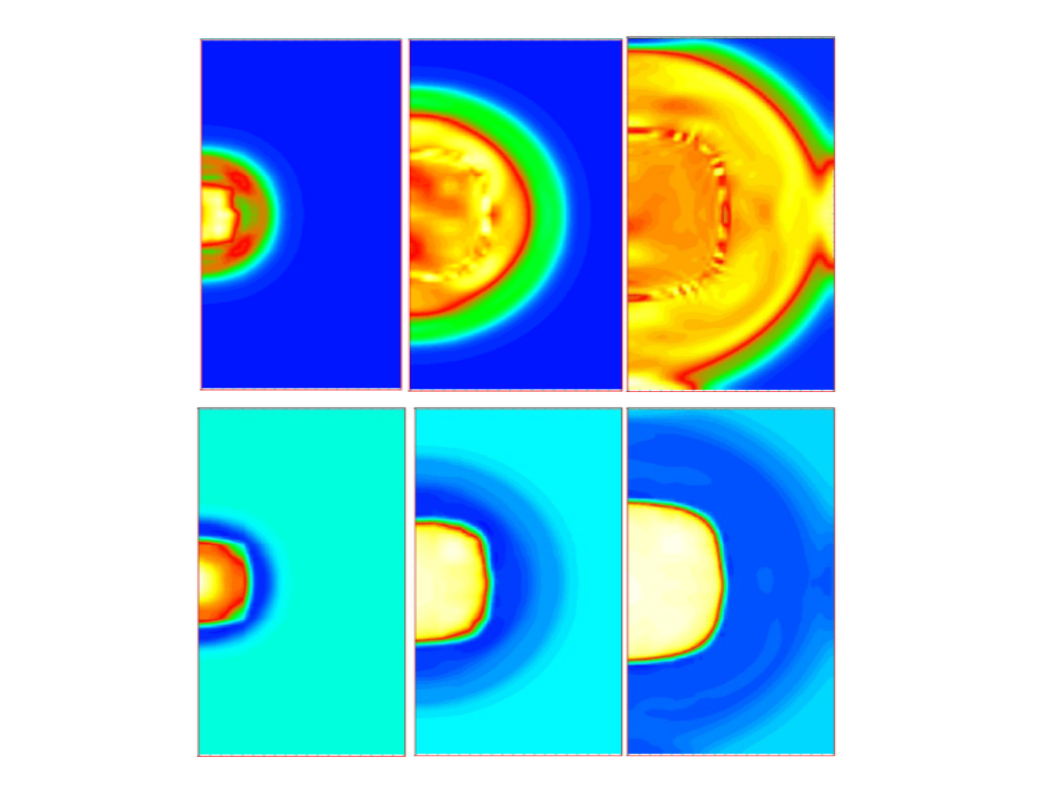
\includegraphics[width=.7\linewidth,height=.5\linewidth,clip]{./Pics/WasteRepos.png}

     \vspace{2cm}
 
     {\Large{\bf \href{tinyurl.com/nlzzbg7}{Jeff Gomes}}}\\
     {\Large{\bf (\href{mailto:jefferson.gomes@abdn.ac.uk}{jefferson.gomes@abdn.ac.uk})}}

     \vspace{1cm}
      {\Large{\bf \href{https://www.abdn.ac.uk/engineering/research/environmental-industrial-fluid-mechanics-122.php}{Mechanics of Fluids, Soils and Structures Research Group}}}
      {\Large{\bf \href{https://www.abdn.ac.uk/engineering/}{School of Engineering}}}\\
      {\Large{\bf \href{https://goo.gl/maps/q3uF9gKyLTN2}{AB24 3UE}}}



     \vspace{2cm}
     {\Large{\bf February, 2018}} %\today}}
  \end{center}

\clearpage

\vbox{
\vspace{18cm}
\begin{description}
  \item[Figure:] Numerical simulation of hypothetical criticality event in nuclear waste repositories. Energetic transients involving extinct fissile material and water surrounded by homogeneous rock matrices (coupled solid-vapour-liquid phase equilibrium and fluid dynamics systems). Extracted from J.L.M.A. Gomes (2009) 'FETCH: A Multi-scale and Multiphysics Model Framework for Nuclear Applications' presented at the 'Todai Forum 2009: Role of Nuclear Energy for Sustainable Development', Imperial College London, UK.
\end{description}}  
\pagenumbering{gobble}% Remove page numbers (and reset to 1)

\end{titlepage} 

%\pagenumbering{roman}% Arabic page numbers (and reset to 1)
\clearpage

\pagenumbering{gobble}% Remove page numbers (and reset to 1)

\pagenumbering{roman}% Arabic page numbers (and reset to 1)
\begin{center}
  \Large{ \bf Revisions}

\bigskip

\begin{tabular}{ c c}
\hline
                         &                    \\
                         &                    \\
{\bf Revision number}    & {\bf Date }        \\
\hline
  0                      & March 10$^{\text{th}}$, 2018 \\
\hline 
\end{tabular}
\end{center}

\setcounter{page}{1}

\tableofcontents
\vfill
%%%% ETOC
\etocarticlestyle 

\pagebreak
\listoftables
\vfill
\pagebreak 
\listoffigures
\vfill
\pagebreak 

\pagenumbering{arabic}% Arabic page numbers (and reset to 1)

\makeatletter\@openrightfalse 
\extraPartText{\blue{(Contents of this Part are not examinable. They were designed to help with some of the notations and definitions used in the remaining of this Notes.)}} 
\part{Fundamentals of Thermodynamics: Introduction and Review of Basic Concepts}
  
%%%
%%% CHAPTER
%%%
\chapter{Thermodynamics: Introduction and Principles}\label{Chapter:Introduction}


   \begin{LearningObjectivesBlock}{Learning Objectives}
      Upon completion of this chapter, you will
        \begin{enumerate}
           \item be able to identify the main elements in a thermodynamic system;
           \item understand the concept of thermodynamic equilibrium;
           \item be able to state the zeroth law of thermodynamics.
        \end{enumerate}
\medskip
     Recommended reading: Chapter 2 of \citet{Atkins_Book,Devoe_Book,Borgnakke_Book}.
   \end{LearningObjectivesBlock}

%%%% ETOC
\etocsetnexttocdepth{subsection}
\localtableofcontents

%%%
%%% SECTION
%%%
   \section{Introduction}\label{Chapter:Introduction:Section:Introduction}

   The word `{\it thermodynamics}' stems from Greek roots, {\it therme}: heat and {\it dynamis}: power -- `movement of heat', and was used by the first time by Lord Kelvin \citep{Thomson_1849}. Thermodynamics studies global properties of the matter and the process (\eg thermal, chemical, mechanical, nuclear etc) in which these properties may be altered. In other words, the quantification of the inter-relation between energy and the change of properties of any physical system.

   For most practical applications, thermodynamics deals with interactions between thermal (\ie heat and temperature), mechanical (\ie work) and/or chemical (\ie chemical potential) energies. \citet{Borgnakke_Book} defined thermodynamics as the `the science that deals with heat and work and those properties of matter that relate to heat and work.'

   \medskip
   
   The study of thermodynamics may be divided into two main areas, {\it classical} and {\it statistical} thermodynamics. The latter investigates the macroscopic properties of systems comprising of a large number of subsystems (\ie particles or atoms). Properties of such systems are controlled by the motion of each set (or assembly) of particles, which can be determined by applying probabilistic theories and methods to laws of motion.

   {\it Classical thermodynamics} studies macroscopic changes of properties, \ie it is assumed that matter is formed by large quantity of particle assemblies that have properties representing the interactions between these assemblies. The extent of such changes due to transfer of energy to or from the system is described by fundamental equations of thermodynamics which are derived from observations known as `{\it Laws of Thermodynamics}'. These laws are postulates that describe the nature of interactions of systems and energy.

   {\bf This document will focus only on the study of fundamentals of \underline{classical thermodynamics} and its application on environmental and industrial problems. }

%%%
%%% SECTION
%%%
   \section{Main Elements of Thermodynamics Analysis}\label{Chapter:Introduction:Section:ThermodAnalysis}

   The first stage in the analysis of any thermodynamic problem is to identify the domain in which all energy and/or forces are transferred to or from.
% Figure
   \begin{figure}[h]
     \begin{center}
       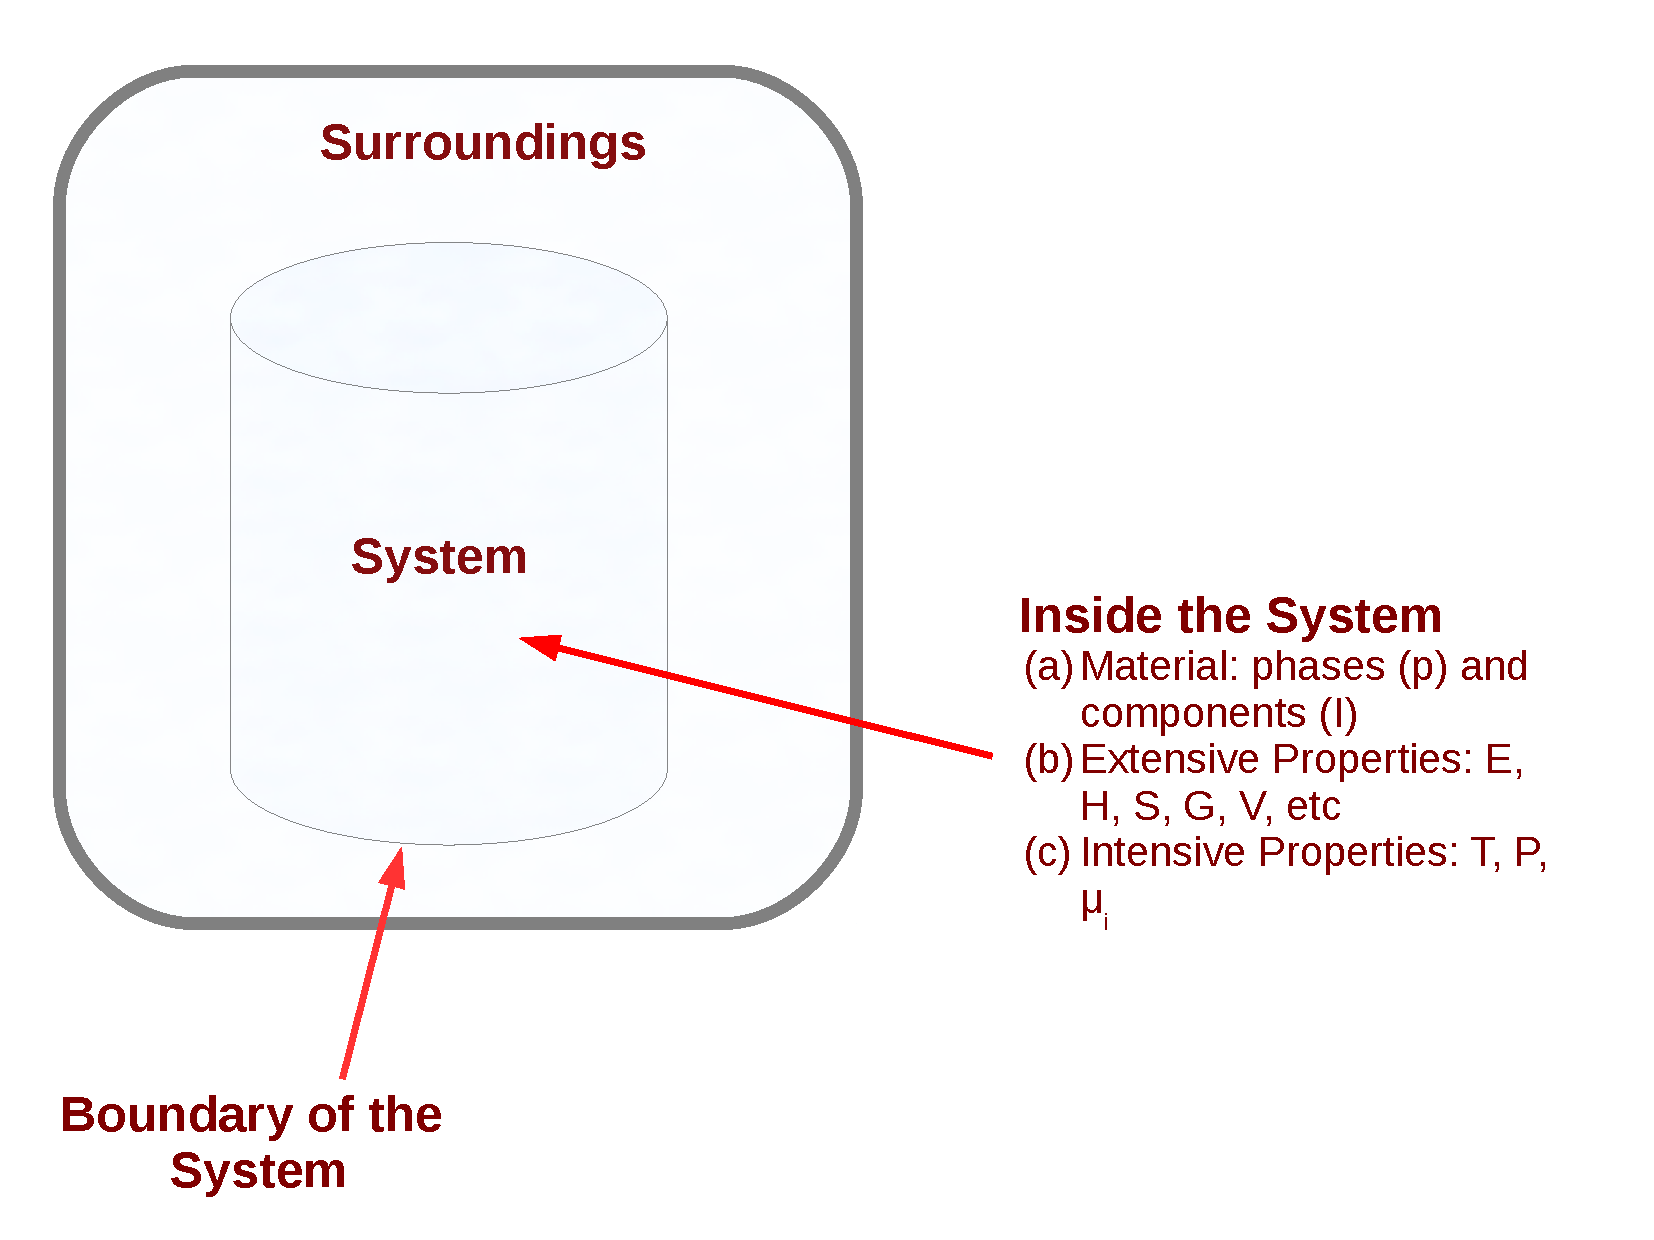
\includegraphics[width=8cm, height=8cm]{./Pics/Fig_SystemDefinition}
       \caption{Elements of a thermodynamic problem: system and surroundings separated by well-defined borders.}\label{Chapter:Introduction:Fig:Domain}
     \end{center}
   \end{figure}
   
   
%%% Subsection
   \subsection{System, Surroundings and Boundaries}\label{Chapter:Introduction:Section:Introduction:SystemSurroundingsBoundaries}\index{System}\index{System!Boundaries}\index{System!Surroundings}
   In practice, any thermodynamic analysis starts by defining the domain of interest, which can be a volume in space or quantity of matter (Fig.~\ref{Chapter:Introduction:Fig:Domain}). This domain is called {\it system}, \ie any 3-D region of physical space with prescribed mass; the remaining of the domain is called {\it surroundings} (or {\it neighbourhood}) which is limited by {\it boundaries}. The {\it boundary} is a surface that encloses the {\it system} and separates it from the {\it surroundings}. For example, in Fig.~\ref{Chapter:Introduction:Fig:Domain2}, liquid nitrogen is contained in a cylinder with prescribed wall thickness. In this case, the interior of the vessel with N$_{2}$ is the {\it system}, whereas the cylinder wall is the border of the system. 
% Figure
   \begin{wrapfigure}{I}{0.5\columnwidth}
        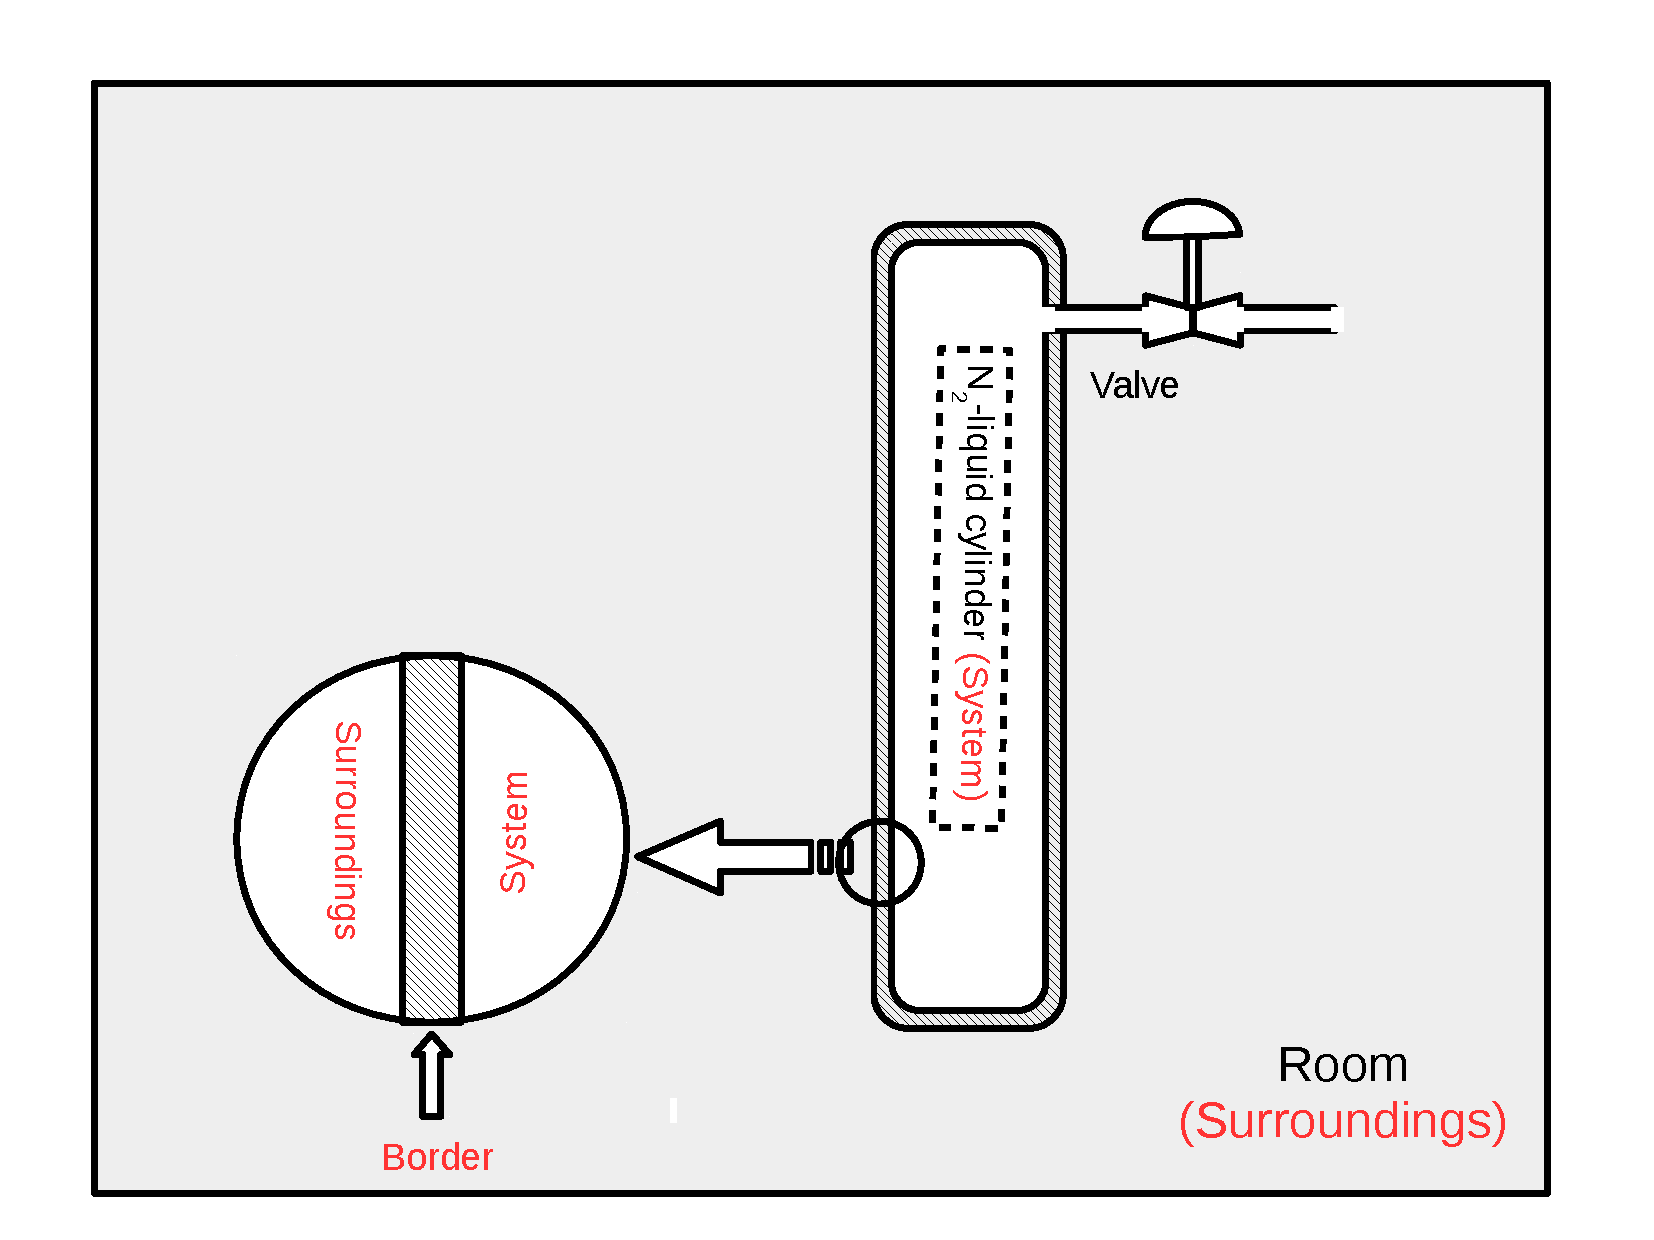
\includegraphics[width=0.4\columnwidth,clip]{./Pics/Fig_SystemDefinition2}
        \caption{Example of a well-defined thermodynamic problem: cylinder stored in a room. Pressurised liquid N$_{2}$ contained in a cylinder is the system, whereas the remaining of the room are the surroundings. Cylinder's wall is the border of the system.}\label{Chapter:Introduction:Fig:Domain2}
   \end{wrapfigure}

   For convenience, sometimes we may want to divide the {\it system} into multiple {\it sub-systems} and analyse them individually, or to combine several small {\it systems} into larger {\it super-systems}. The choice depends on the conditions of the domain of interest and how mass and energy flow across the {\it sub-systems}. For example, in Fig.~\ref{Chapter:Introduction:Fig:Domain2}, if the valve is opened to the room (at atmospheric pressure) $N_{2}$ would be vaporised ({\it phase change}) and occupy the whole room. In such scenario, the room and the cylinder become the {\it system} bounded by the room's walls; the area outside the room is now the surroundings. Multiple different configurations can be drawn from this rather simple cylinder-room set.

%%% Table
   \begin{table}[h]
     \begin{center}
      \begin{tabular}{|c|c|c|}
         \hline
                      & {\bf Mass} & {\bf Energy} \\
                      & {\bf Exchange} & {\bf Exchange} \\
         \hline
         {\bf Open}   & {\it yes}  & {\it yes}    \\
         {\bf Closed} & {\it no}   & {\it yes}    \\
         {\bf Isolated}&{\it no}   & {\it no}     \\
         \hline 
      \end{tabular}  
        \caption{System and control volumes: energy and mass transfer.}\label{Chapter:Introduction:Table:System}
     \end{center}
   \end{table}
   
   If mass and energy are allowed to flow across the {\it boundaries}, we say that the {\it system} is {\bf open}, otherwise if only the energy is allowed to flow (\ie be transferred) across the {\it boundaries}, the {\it system} is assumed to be {\bf closed}. If both energy and mass can not be transferred across the {\it boundaries} the system is assumed {\bf isolated}, in such case, where there is no energy flow, the boundary is called {\bf adiabatic} (Table~\ref{Chapter:Introduction:Table:System}).\index{System!Open}\index{System!Closed}\index{System!Isolated}\index{System!Adiabatic}\index{Adiabatic}

% Figure
   \begin{figure}[h]
     \begin{center}
        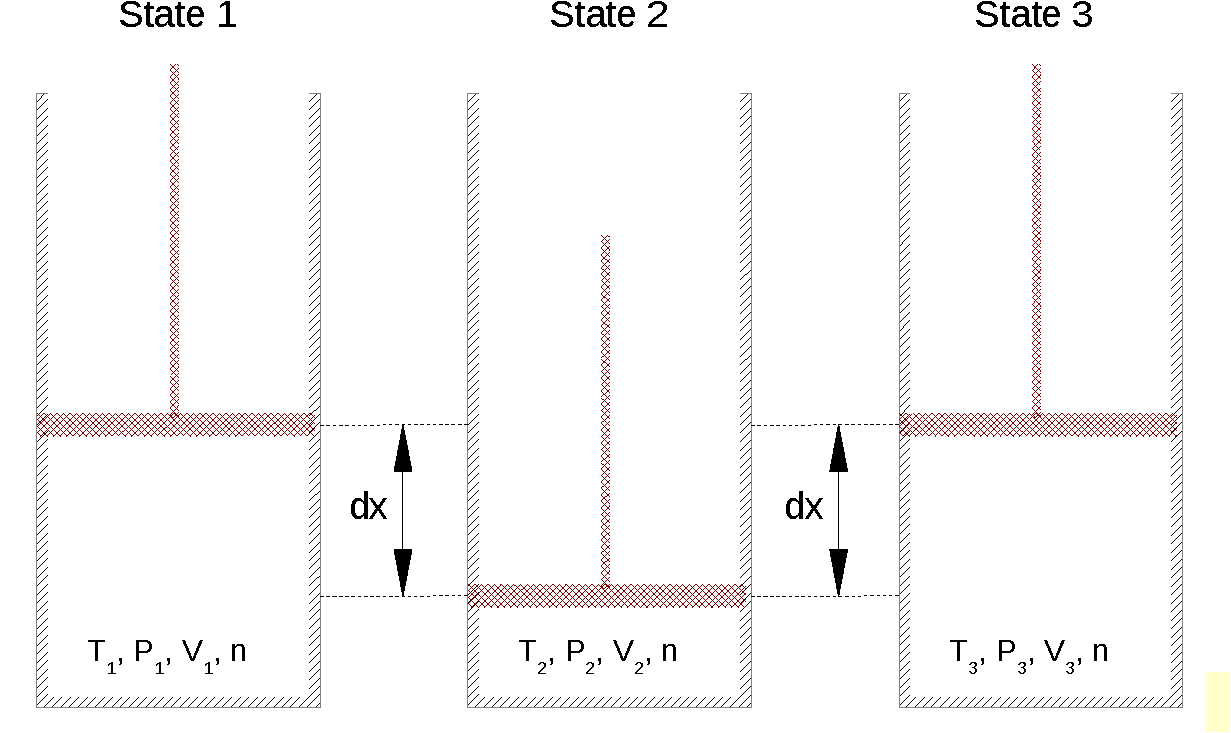
\includegraphics[width=0.7\columnwidth,clip]{./Pics/Fig_SystemDefinition3}
        \caption{Cylinder-piston system with extensive/intensive properties.}\label{Chapter:Introduction:Fig:Domain3}
     \end{center}
   \end{figure}

   In the example depicted in Fig.~\ref{Chapter:Introduction:Fig:Domain2}, assuming an ordinary industrial liquid N$_{2}$ (at subzero temperature) cylinder, if the valve is closed, then there is no fluid flow from the cylinder to the room, but heat is flowing from the environment to the cylinder cavity. Such system is said to be {\bf closed}.
   
\medskip
% Example
\begin{MyExample}{\begin{center}{\bf Example}\end{center}}
\begin{example}\label{Chapter:Introduction:Example1}
  \citep{Reisel_Book} For the following systems, determine whether the system described is best modelled as an isolated, closed or open system:
  \begin{enumerate}[a)]
     \item steam flowing through a turbine\;\;$\rightarrow$\;\; {\it Open.}
     \item an incandescent light bulb\;\;$\rightarrow$\;\; {\it Closed.}
     \item an inflated tire\;\;$\rightarrow$\;\; {\it Isolated if the tire is at rest, but closed if it is in movement.}
     \item a rock formation 200 m below the surface of the earth\;\;$\rightarrow$\;\; {\it Open.}
     \item a tea kettle containing boiling water\;\;$\rightarrow$\;\; {\it Open as water steam can still leave the system.}
     \item a human body\;\;$\rightarrow$\;\;{\it Depending on the circumstances, a human body can be either open (\eg during meals, physical exercises etc) or closed.}
     \item an engine's radiator\;\;$\rightarrow$\;\; {\it Closed}.
  \end{enumerate}
\end{example}
\end{MyExample}

%%% Subsection
   \subsection{Properties and State of Substances}\label{Chapter:Introduction:Section:Introduction:ExtensiveIntensiveProperties}\index{Extensive Properties}\index{Intensive Properties}\index{System!Extensive Properties}\index{System!Intensive Properties}
   The {\it material} in a system is composed of phases (e.g., solid, liquid, gas) with distinct physical and chemical properties, thus with explicit {\it boundaries} (\ie interfaces) between phases. {\it State} is the condition of the system at an instant of time and described by its properties.  From this definition of state, any property has a single value at each state. A quantitative property of a system (\eg temperature and pressure) describes macroscopic characteristics, which may vary with time (\ie time-dependent property). Two states of the matter are equivalent if they have the same properties, \eg in a cylinder-piston system (Fig.~\ref{Chapter:Introduction:Fig:Domain3}) containing {\it n} moles of pure gas, if {\it state 1} is defined by temperature $T_{1}$, pressure $P_{1}$ and volume $V_{1}$, and {\it state 3} is defined by temperature $T_{3}$, pressure $P_{3}$ and volume $V_{3}$, state 1 is {\it equivalent} to state 3 {\it if and only if} $T_{1} = T_{3}$ and $P_{1} = P_{2}$. 
\medskip

   Thermodynamic properties may be classified as either {\bf extensive} or {\bf intensive}. An extensive property is a property that depends on the mass (or extent) of the substance (\ie size) in the system. Examples of extensive properties are total mass, total volume, total internal energy etc. An intensive property is a property that is independent of the mass of the substance, examples are temperature and pressure.
% Figure
   \begin{wrapfigure}{R}{0.5\columnwidth}
        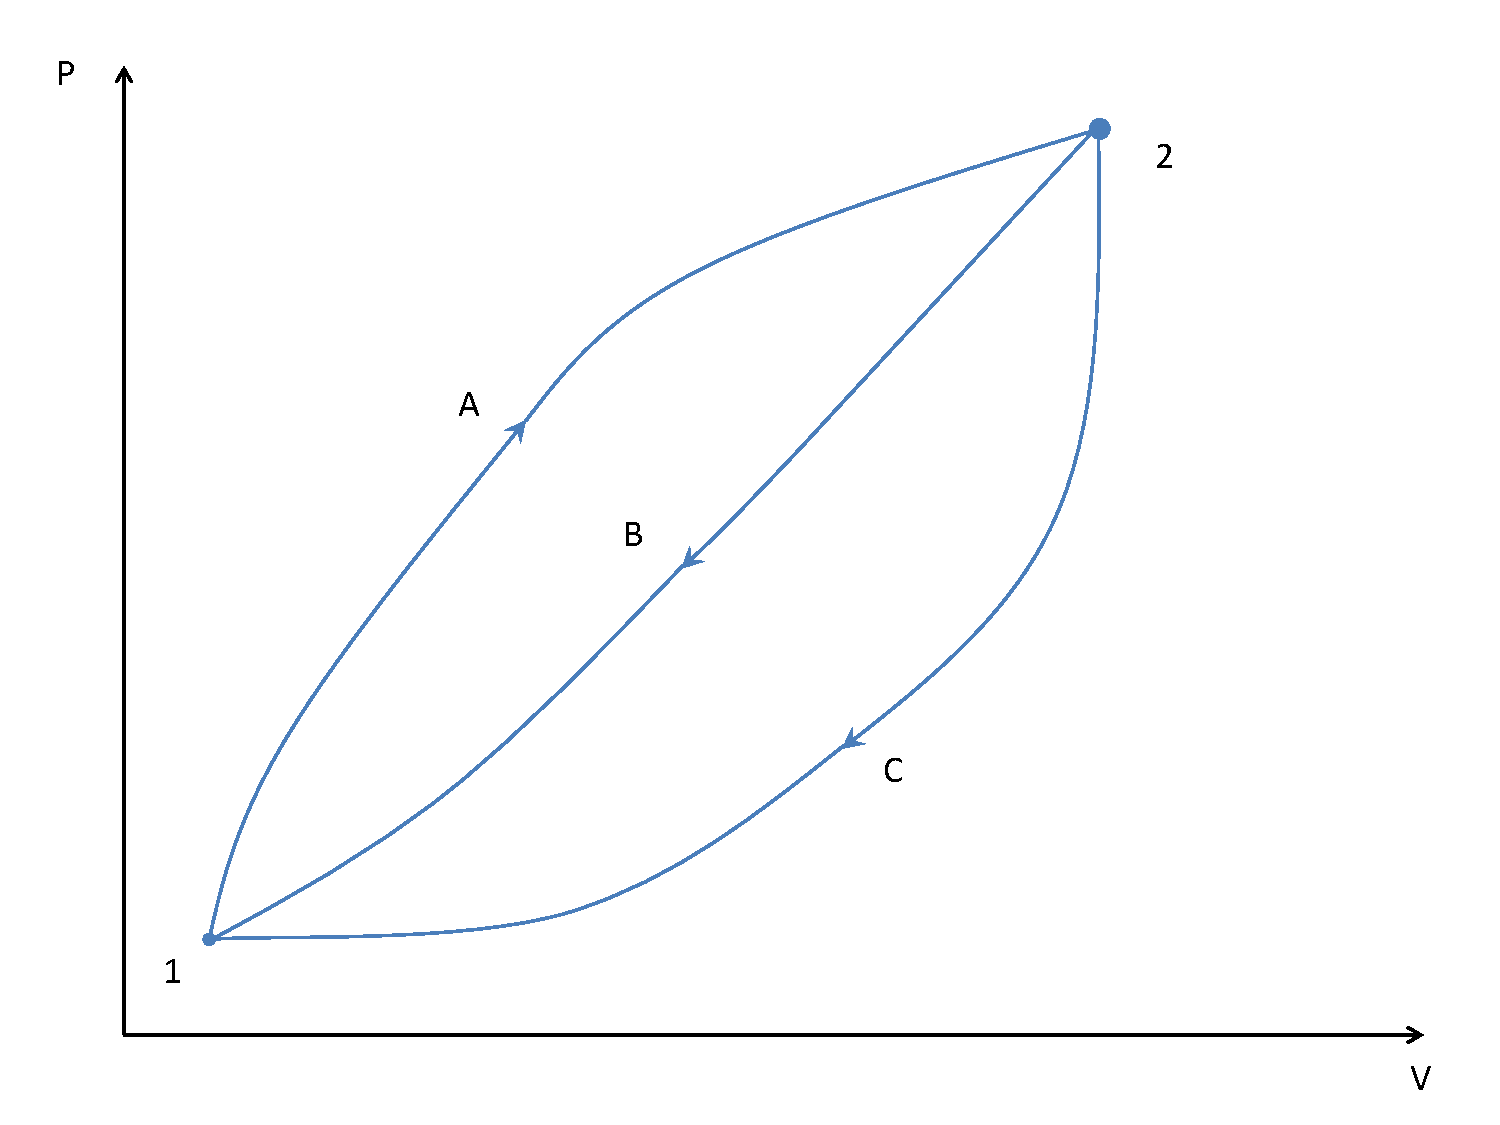
\includegraphics[width=0.4\columnwidth,clip]{./Pics/first_law_process}
        \caption{Schematic representation of cycles.}\label{Chapter:Introduction:Fig:CyclesSchematic}
   \end{wrapfigure}

   Thus, for example, if a system is cut in half, its intensive properties remain unchanged, while extensive properties are cut in half. The ratio of an extensive property to the mass (\ie property per unit mass) is called {\bf specific property}, and this is an {\bf intensive} property.. The ratio of an extensive property to the number of moles of the substance in the system (\ie property per mole) is referred as {\bf molar property}, this is also an {\bf intensive} property.

%%% Subsection
   \subsection{Processes and Cycles}\label{Chapter:Introduction:Section:Introduction:ProcessesCyclesDefinition}\index{Process}\index{Cycle}
   A process occurs when the system undergoes a change in a state or a transfer of energy at a steady-state. For example, let's consider the cylinder-piston system (Fig.~\ref{Chapter:Introduction:Fig:Domain3}) at state 1. As mechanical energy is transferred from the surroundings through a force (represented by an external pressure) exerted on the piston, the state of the system changes from {\it 1} to {\it 2}. A {\it quasi-static process}\index{Process!Quasi-Static} (also called reversible process) is a succession of equilibrium states at infinite slowness $\left(\Delta\text{t}\rightarrow\text{0}\right)$.
   
   {\it Cycles} are defined as any process (or a set of processes) in which the end states are identical. For example, in the processes (closed system) depicted in Fig.~\ref{Chapter:Introduction:Fig:CyclesSchematic}, the system is initially at state 1 $\left(\text{with coordinates } P_{1}\text{ and }V_{1}\right)$ and driven (by simultaneous changes in pressure, volume and temperature) to the state 2 through pathway $A$. After a while, the system is restored to the original state $1$ through pathway $B$. These two processes, $A$ and $B$, constitute a cycle as the final state is the same as the initial state.   
   
%%%
%%% SECTION
%%%
   \section{Thermodynamic Work and Heat}\label{Chapter:Introduction:Section:ThermodynamicWorkHeat}\index{Work}\index{Heat}\index{Energy}
   \begin{subequations}
     Work can be defined as a form of energy transfer due to changes in external macroscopic physical properties of a thermodynamic system. It can be expressed in several forms: magnetic, mechanical, electrical etc. For example, in a piston-cylinder system (Fig.~\ref{Chapter:Introduction:Fig:Domain3}) work is produced by the system when the gas volume expands against an external force (states 2-3). Similarly, an external force is responsible for the compression of the gas, \ie work is given to the system (states 1-2). In these cases (expansion and compression of a gas), the transfer of work (to or from the system) is due to the application of a finite force on the system boundary (piston).

     It is clear that the boundary (\ie volume limited by the cylinder wall and the piston-head) either contracts or expands due to external and internal forces acting on it. In other words, applied forces acting over a distance (piston length) result in mechanical energy transfer (\ie work). For an infinitesimal displacement of the piston within a cylinder, {\it dx}, the work ($W$) can be defined by
     \begin{equation}
        dW = F dx,\label{Chpt01_Work1}
     \end{equation}
     where $F$ is the force acting vertically upon the piston. If the movement occurs over a finite distance, the resulting work can be obtained by integrating Eqn.~\ref{Chpt01_Work1}. By convention, {\bf work} is assumed {\bf positive} if the displacement is in the same direction as the force applied, and {\bf negative} when the force and the displacement are in opposite directions. Thus, from stages 2 to 3 (Fig.~\ref{Chapter:Introduction:Fig:Domain3}), the force is acting upon the piston with contraction of the volume of the gas $\left(V^{t}\right)$,
     \begin{displaymath}
       dW = -PAd\left(\frc{V^{t}}{A}\right),
     \end{displaymath}
     where $A$ is the area of the piston (constant) and $P=F/A$ is the pressure exerted on the piston, then
     \begin{shaded}
        \begin{equation}
           dW = -PdV^{t}.\label{Chpt01_Work2}
        \end{equation}
     \end{shaded}
     Equation~\ref{Chpt01_Work2} describes the work undertaken by any process when the volume changes due to transfer of energy from or to the system. If the fluid undertakes a compression (thus reduction of volume) due to pressure over the system, the work is positive, otherwise when the system produces work (\ie transfer energy to the surroundings through expansion of the boundaries), the work is considered as negative. The concept of work leads to the definition of {\bf energy} as the capacity of the system to produce work.

     \citet{Devoe_Book} defined {\bf heat} as `the transfer of energy across the boundary caused by a temperature gradient at the boundary'. This concept will naturally lead to the {\it First Law of Thermodynamics} (Chapter~\ref{Chapter:FirstLaw}).     

   \end{subequations}
   
%%%
%%% SECTION
%%%
   \section{Thermodynamic Equilibrium and the Zeroth Law}\label{Chapter:Introduction:Section:Equilibrium_ZerothLaw}\index{Equilibrium!Mechanical}\index{Equilibrium!Chemical}\index{Equilibrium!Thermal }\index{Laws of Thermodynamics!Zeroth law}
   During thermodynamic processes, the state of the system may change due to gradients of different variables within or across boundaries, \ie
   \begin{enumerate}[a)]
        \item pressure gradients result in momentum transfer and/or convective mass transport;
        \item temperature gradients produce heat exchange, and;
        \item concentration gradients yields to diffusive mass transfer.
   \end{enumerate}
   Changes in the state of the system will continue until all internal or cross-boundary gradients vanish. When all gradients are non-existent the system exhibits no further changes and at such conditions, the system is said to be in {\bf thermodynamic equilibrium}.\index{Equilibrium!Thermodynamic}
      A system is in {\bf thermodynamic equilibrium} if it satisfies the criteria for mechanical, thermal and chemical equilibrium.  
% Figure
   \begin{wrapfigure}{I}{0.5\columnwidth}
        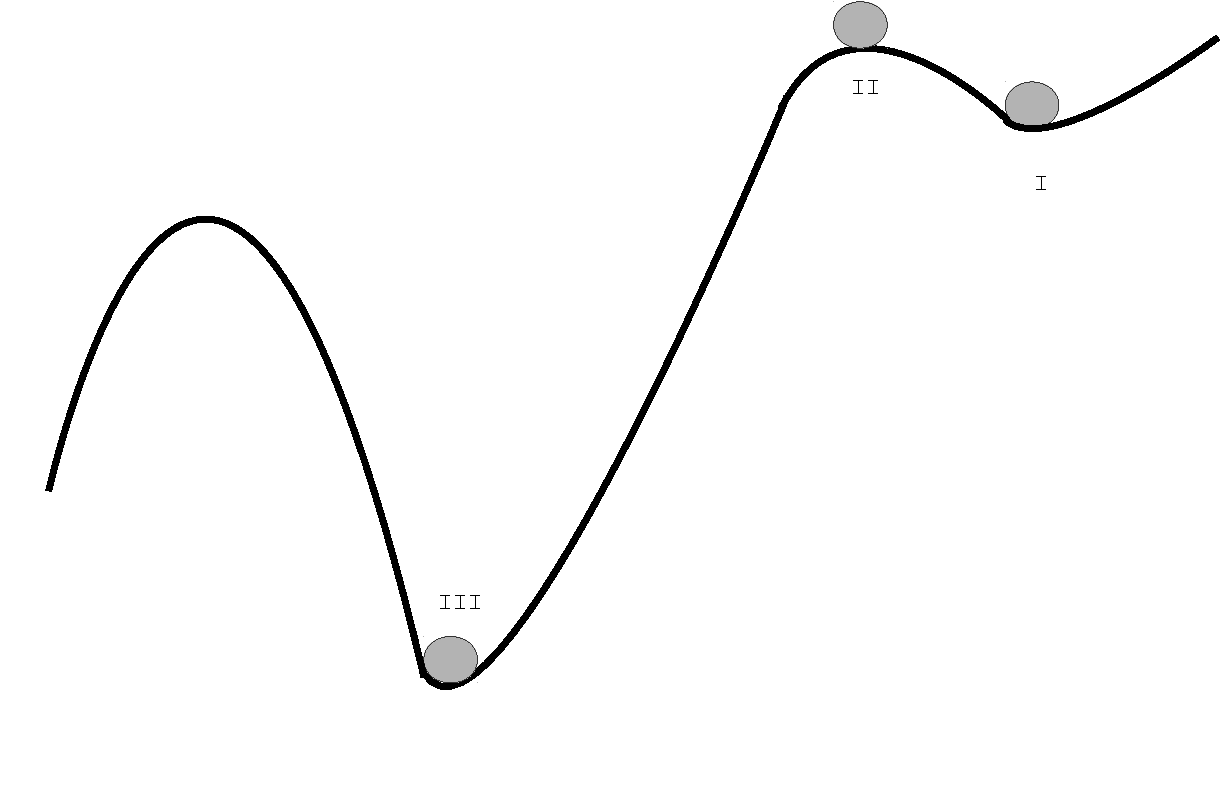
\includegraphics[width=0.4\columnwidth,clip]{./Pics/Fig_SystemDefinition4}
        \caption{Potential energy variation in a particle motion.}\label{Chapter:Introduction:Fig:Domain4}
   \end{wrapfigure}

   Let's consider a particle initially at rest (state I in Fig.~\ref{Chapter:Introduction:Fig:Domain4}). The total energy associated with this particle is the sum of potential and kinetic energies (assuming that the particle is chemically inert and is kept at a constant temperature). If the particle is perturbed by a mechanical force of very small magnitude, it will eventually return to its initial state (\ie at a finite time), however if the perturbation is sufficiently large the particle is unlikely to return to the original state. In this scenario, the particle is said to be in a {\it unstable equilibrium}\index{Equilibrium!Mechanical!Unstable}. Now, let's assume that the particle is at state II, where any perturbation can move it to either state I or III. In such conditions, the particle is said to be in a {\it meta-stable equilibrium}\index{Equilibrium!Mechanical!Meta-stable}. Finally, if the particle is at state III, it will remain at this condition even under the influence of large perturbation. At such conditions, the particle is said to be in a {\it stable equilibrium}\index{Equilibrium!Mechanical!Stable}. If $E_{p}$ is the potential energy of the particle and $x$ is the displacement in the vertical direction, the equilibrium states can be described as
   \begin{equation}
      \begin{cases}
         \text{Stable equilibrium (III):}  & \frc{\partial E_{p}}{\partial x} = 0 \text{ and } \frc{\partial^{2} E_{p}}{\partial x^{2}} > 0; \\
          \\
         \text{Unstable equilibrium (II):}  & \frc{\partial E_{p}}{\partial x} = 0 \text{ and } \frc{\partial^{2} E_{p}}{\partial x^{2}} < 0; \\
          \\
         \text{Meta-stable equilibrium (I):}  & \frc{\partial E_{p}}{\partial x} = 0 \text{ and } \frc{\partial^{2} E_{p}}{\partial x^{2}} = 0; \\
      \end{cases}
   \end{equation}
   These mechanical equilibrium states can be extended to thermodynamic systems during phase changes, where the potential energy and the spatial coordinate are replaced by the {\it Gibbs free energy} and intensive/extensive properties, respectively.

   \bigskip

   The concept of thermal equilibrium is intuitively simple: if two or more bodies at distinct temperatures are in physical contact, the bodies will tend to a single temperature at a finite time. This principle is called the {\bf Zeroth Law} of thermodynamics and was first stated by J. C. Maxwell in 1872:
   \begin{MyBlock}{{\bf Zeroth Law of Thermodynamics (Maxwell, 1872) } }
     ``Bodies whose temperatures are equal to that of the same body have themselves equal temperatures.”
   \end{MyBlock}
   This definition enables the use of thermometers as devices to measure the temperature of bodies. Traditional thermometers have two components, a bulb containing mercury and a linear temperature scale. The mercury bulb is maintained at a relatively low temperature $\left(\text{\ie } T_{\text{th}}\le 35^{\circ}\text{C}\right)$, whereas a body is at temperature $T>T_{\text{th}}$. When the thermometer and the body are in contact, from the {\it zeroth law}, both will reach the same temperature $T$ at a finite time. The temperature difference triggers a volumetric expansion of the mercury that can be readily observed in the scaled glass column.

\clearpage   
\begin{FinalSummaryBlock}{Summary}
    In this chapter, some fundamental concepts of thermodynamic properties were revised and the their relationships with energy were introduced, also:
    \begin{itemize}
       \item Thermodynamics is the study of the transformations of energy;
       \item Energy can be defined as the capacity to produce work;
       \item Work is the transfer of energy by motion against an opposing force (Eqns.~\ref{Chpt01_Work1}-\ref{Chpt01_Work2};
       \item Heat is the transfer of energy  as a result of a temperature difference between the system and the surroundings;
       \item Definitions of system, surroundings and boundaries were stated in Section~\ref{Chapter:Introduction:Section:Introduction:SystemSurroundingsBoundaries};
       \item In open systems, mass and energy are allowed to freely flow across the boundaries of the system, whereas in closed system only energy is able to cross the borders at constant mass. In isolated (or adiabatic) system, neither energy nor mass can be trabsported across the borders;
       \item A state function is a property that depends only on the current state of the system and is independent of the origin of the state; 
       \item Thermal equilibrium is a condition in which no change of state occurs when two (or more) bodies are in contact with each other;
       \item Mechanical equilibrium is the condition of equality of pressure across the boundary of the system;
       \item The Zeroth Law of thermodynamics states that if a body {\it A} is in thermal equilibrium with a body {\it B}, and {\it B} is in thermal equilibrium with {\it C}, then {\it C} and {\it A} are also in thermal equilibrium;
    \end{itemize} 
   
     Most of these fundamentals concepts are familiar to you through other engineering courses. However, the remaining of this document strongly relies on this concepts and ideas, and you should understand all these concepts before moving forward.
\end{FinalSummaryBlock}

%\begin{MyTutorial}{\begin{center}{\bf Tutorial}\end{center}}
%  \begin{problem}
%  \end{problem}
%\end{MyTutorial}
 % Introduction and Review of Basic Concepts of Thermodynamics
     \setcounter{examplecounter}{0}
  
%%%
%%% CHAPTER
%%%
\chapter{Introduction to Properties of Gases}\label{Chapter:Intro_Property_of_Gases}

   \begin{LearningObjectivesBlock}{Learning Objectives}
      Upon completion of this chapter, you will be able to
        \begin{enumerate}
           \item define ideal gas and identify the main assumptions;
           \item differentiate an ideal from a real gas through state conditions;
           \item explain Boyle's, Gay-Lussac's and Charles' laws for ideal gases;
           \item define and explain the equation of state for ideal gases;
           \item state the Dalton's law for gaseous mixtures.
        \end{enumerate}
\medskip
     Recommended reading: Chapter 1 of \citet{Atkins_Book,Adamson_BookChapter}.
   \end{LearningObjectivesBlock}


%%%% ETOC
\localtableofcontents
   
%%%
%%% SECTION
%%%
     \section{Introduction}\label{Chapter:Intro_Property_of_Gases:Section:Intro}

   The physical condition (\ie state) of a substance is defined by its physical properties. For example, the state of a pure fluid is specified by volume ($V$), mass (through the number of moles, $n$), pressure ($P$) and temperature ($T$). Laboratory experiments with fluids revealed that if three of these properties (\eg $V, n, T$) are specified, the state of the fluid is naturally defined, and the forth property (\ie $P$) is fixed. Mathematically, this can be represented by a functional often referred as {\bf equation of state}\index{Equation of State} (EOS)\index{EOS|see {Equation of State}},
     \begin{displaymath}
       P = f(T,V,n),
     \end{displaymath}
     which states that if $T$, $n$ and $V$ are known for a particular fluid, then the pressure of the system for the fluid at this state can be readily determined. The state and properties of any chemical species can be described by an specific equation of state\footnote{Equations of state are the main focus of Chapter~\ref{Chapter:VolumetricPropertiesPureSubstances}.}.
   
%%%
%%% SECTION
%%%
     \section{Ideal Gases}\label{Chapter:Intro_Property_of_Gases:Section:IdealGases}\index{Gases!Ideal gas}
     \begin{subequations}

     \noindent A fluid is assumed to behave as an {\it ideal gas} if the following two assumptions are true:
     \begin{enumerate}[i)]
       \item molecules of gases are considered as {\bf massless} particles;
       \item there are {\bf no} interaction between the gas particles due to,
         \begin{enumerate}[a)]
           \item volume of the molecules is negligibly small compared with the volume occupied by the gas, and/or;
           \item the distance between gaseous molecules are infinitely large $\left(d\rightarrow \infty\right)$, except during elastic collisions over negligible duration.
         \end{enumerate}
     \end{enumerate}
     \noindent These lead to an obvious conclusion that for a gas to behave as an ideal gas the pressure should be infinitely small, \ie $P\rightarrow 0$. In practical engineering calculations, we assume that a fluid behaves as an ideal gas at low to moderate pressures. The $PVT$ behaviour of fluids was initially investigated through experimental observations of gases at low pressures that led to three intuitive relationships:
     \begin{itemize}
       \item For isothermal processes in closed systems (\ie $T$ and $n$ are constant), $P$ and $V$ are inversely proportional to each other, \ie an increase in pressure leads to a decrease in volume,
          \begin{displaymath}
             P \propto \frc{1}{V},
          \end{displaymath}          
%          
       \item For isochoric processes in closed systems (\ie $V$ and $n$ are constant), $T$ and $P$ are directly proportional to each other, \ie an increase in temperature leads to an increase in pressure,
          \begin{displaymath}
            T \propto P,
          \end{displaymath}         
%
       \item For isobaric processes in closed systems (\ie $P$ and $n$ are constant), $T$ and $V$ are directly proportional to each other, \ie an increase in temperature leads to an increase in volume.
          \begin{displaymath}
            T\propto V.
          \end{displaymath}          
     \end{itemize}
     \begin{shaded}
        These proportionality relations can be merged into a single expression,\index{Gases!Boyle's law}\index{Gases!Gay-Lussac's law}\index{Gases!Charles' law}\index{Gay-Lussac's law|see {Gases}}\index{Charles' law|see {Gases}}\index{Boyle's law|see {Gases}}
          \begin{equation}
            \frc{P V}{n T} = R \;\;\Longleftrightarrow \;\;
              \begin{cases}
                P_{1}V_{1} = P_{2}V_{2}, & \text{if } T \text{ and } n \text{ are constant (Boyle's law)},  \\
         \\
                P_{1}T_{1}^{-1} = P_{2}T_{2}^{-1}, & \text{if } V \text{ and } n \text{ are constant (Gay-Lussac's law)}, \\
         \\
                V_{1}T_{1}^{-1} = V_{2}T_{2}^{-1}, & \text{if } P \text{ and } n \text{ are constant (Charles' law)}.
             \end{cases}\label{Chapter:Intro_Property_of_Gases:Eqn:IdealEOS}\index{Equation of State!Ideal gas}
          \end{equation}
        The constant of proportionality, $R$, which is found experimentally to be the same for all gases, is called {\bf universal gas constant} (Table~\ref{Chapter:Intro_Property_of_Gases:Table:RConst}). This expression, 
          \begin{equation}
             P=\frc{n R T}{V},\label{Chapter:Intro_Property_of_Gases:Eqn:IdealEOS}\index{Equation of State!Ideal gas}
          \end{equation}\index{Equation of State!Ideal gas}
        is called {\bf ideal gas equation of state} and becomes increasingly accurate for any gas as pressure tends to zero $\left(P\rightarrow 0\right)$.
     \end{shaded}
     \end{subequations}
     
   \begin{table}[h]
     \begin{center}
     \begin{tabular}{||c c||}
       \hline\hline
           $\mathbf{R}$   & {\bf Units} $\mathbf{\left(\text{V.P.T}^{-1}\text{n}^{-1}\right)}$ \\
           \hline\hline
           8.3145    &  J.K$^{-1}$.mol$^{-1}$  \\
           8.3145    &  kJ.K$^{-1}$.kmol$^{-1}$  \\
           8.3145    &  l.kPa.K$^{-1}$.mol$^{-1}$  \\
           8.3145$\times$10$^{-3}$    & cm$^{3}$.kPa.K$^{-1}$.mol$^{-1}$  \\
           8.3145    &  m$^{3}$.Pa.K$^{-1}$.mol$^{-1}$  \\
           8.3145$\times$10$^{-5}$    &  m$^{3}$.bar.K$^{-1}$.mol$^{-1}$  \\
           8.2057$\times$10$^{-2}$ &  l.atm.K$^{-1}$.mol$^{-1}$  \\
           \hline\hline           
     \end{tabular}
     \caption{Gas constant, $R$.}\label{Chapter:Intro_Property_of_Gases:Table:RConst}\index{Universal gas constant}\index{R|see {Universal gas constant}}\index{Gas constant|see {Universal gas constant}}
     \end{center}
   \end{table}
   
   % Example
   \begin{MyExample}{\begin{center}{\bf Example}\end{center}}
     \begin{example}\label{Chapter:Intro_Property_of_Gases:Example1}
       In an industrial process, nitrogen is heated to 650.15 K in a vessel of constant volume. If it enters the vessel at 43 atm and 298.15 K, what pressure would it exert at the working temperature if it behaved as an ideal gas?

       {\it This problem deals with a gas that undertakes an isochoric (\ie constant volume) process. Nitrogen gas at $P_{1} = 43$ atm and $T_{1} = 298.15$ K is compressed to pressure $P_{2}$ 'till temperature reaches $T_{2} = 650.15$ K.

         Using the ideal gas equation for states 1 and 2,}
       \begin{eqnarray}
         && \left(\frc{PV}{nT}\right)_{1} = R = \left(\frc{PV}{nT}\right)_{2},\;\;\;\text{ with } V_{1}=V_{2} \text{ and }\;\; n_{1}=n_{2}\nonumber \\
         && \frc{P_{1}}{T_{1}} = \frc{P_{2}}{T_{2}} \;\;\Rightarrow \;\; P_{2}= 93.7664 \text{ atm } \nonumber
         \end{eqnarray}
     \end{example}
   \end{MyExample}

\medskip
   % Example
   \begin{MyExample}{\begin{center}{\bf Example}\end{center}}
     \begin{example}\label{Chapter:Intro_Property_of_Gases:Example2}
       500 kg of helium gas is stored in a tank at 50$^{\circ}$C and 2.5 bar. The fluid is then transferred to a pressure vessel where it is isothermically compressed to 73 bar.  What is the volume occupied by {\it He} in such conditions? Assume ideal gas behaviour. Molar mass ({\it MW}) of helium is 4.0026 g.mol$^{-1}$.

       {\it In this problem, we need to calculate the volume of helium at the pressure vessel after isothermal compression. However, not all necessary conditions are known, \ie}
       \begin{displaymath}
         \frc{P_{1}V_{1}}{n_{1} R T_{1}} = \frc{P_{2}V_{2}}{n_{2} R T_{2}} \Longrightarrow P_{1}V_{1} = P_{2}V_{2},\;\;\;\;\text{where }R\text{ and } n_{i}\text{ are constants},
       \end{displaymath}
           {\it thus there is 1 equation and 2 unknowns, $V_{1}$ and $V_{2}$. In order to solve this problem, we need to first compute $n_{1}$ and $V_{1}$ via, }
           \begin{displaymath}
              V_{1} = \frc{n_{1}R T_{1}}{P_{1}} = 1342.5427\;\text{m}^{3},\;\;\;\text{ where } n_{1} = \frc{m_{1}}{MW_{1}} =  124918.8028\text{ moles}.
           \end{displaymath}
           {\it With $V_{1}$, we can now calculate the volume after compression, $V_{2}$}
           \begin{displaymath}
              P_{1}V_{1} = P_{2}V_{2} \;\;\; \Longrightarrow\;\;\; V_{2} = 45.9775 \text{m}^{3}
           \end{displaymath}
           
     \end{example}
   \end{MyExample}
   
   % Example
   \begin{MyExample}{\begin{center}{\bf Example}\end{center}}
     \begin{example}\label{Chapter:Intro_Property_of_Gases:Example3}
       \citep{Atkins_Book} 
       \begin{enumerate}[a)]
           \item Deduce a relation between pressure and mass density $\left(\rho\right)$ of an ideal gas of molar mass $MW$;
           \item After careful measurement of the density of dimethyl ether at relatively low pressure conditions, a chemical engineering student obtained the following experimental data at 25$^{\circ}$C,
               \begin{center}
                  \begin{tabular}{c c c c c c}
                     $\mathbf{P}$ [kPa]  & 12.223 & 25.20 & 36.97 & 85.23 & 101.3 \\
                     $\mathbf{\rho}\;\left[\text{kg.m}^{-3}\right]$ & 0.225  &  0.456  &  0.664 & 1.468 & 1.734  
                  \end{tabular}
               \end{center}
               Obtain the molar mass of dimethyl ether at each pressure coordinate and compare with the real value of 46.07 g.mol$^{-1}$. What conclusions could be drawn from this data?
       \end{enumerate}
\medskip

       \begin{enumerate}[a)]
           \item {\it The first part of the problem requires the development of a mathematical relation between $P$ and $\rho$. Defining} $\rho=\frc{m}{V}$ {\it which can be allocated in the ideal EOS} $\left(\text{ and }n=\frc{m}{MW}\right)$,
              \begin{eqnarray}
                 P &=& \frc{n R T }{V} = \frc{m}{MW}\frc{R T}{V} \nonumber\\ 
                   &=& \frc{\rho R T}{MW}\nonumber
              \end{eqnarray}
%
           \item {\it We can use the relation derived in part (a) to calculate the molar mass of dimethyl ether at each pressure coordinate, thus}
              \begin{displaymath}
                  \begin{cases}
                     MW_{1} = \frc{\rho_{1} R T}{P_{1}} = \frc{0.225\text{ kg.m}^{-3}\cdot 8.3145\text{ m}^{3}\text{.Pa.}\left(\text{K.mol}\right)^{-1}\cdot 298.15\text{ K}}{12.223\times 10^{3}\text{ Pa}} = 45.6326 \text{ g.mol}^{-1} \\
                     MW_{2} = \frc{\rho_{2} R T}{P_{2}} = \frc{0.456\text{ kg.m}^{-3}\cdot 8.3145\text{ m}^{3}\text{.Pa.}\left(\text{K.mol}\right)^{-1}\cdot 298.15\text{ K}}{25.20\times 10^{3}\text{ Pa}} = 44.8575 \text{ g.mol}^{-1} \\
                     MW_{3} = \frc{\rho_{3} R T}{P_{3}} = \frc{0.664\text{ kg.m}^{-3}\cdot 8.3145\text{ m}^{3}\text{.Pa.}\left(\text{K.mol}\right)^{-1}\cdot 298.15\text{ K}}{36.97\times 10^{3}\text{ Pa}} = 44.5235 \text{ g.mol}^{-1} \\
                     MW_{4} = \frc{\rho_{4} R T}{P_{4}} = \frc{1.468\text{ kg.m}^{-3}\cdot 8.3145\text{ m}^{3}\text{.Pa.}\left(\text{K.mol}\right)^{-1}\cdot 298.15\text{ K}}{85.23\times 10^{3}\text{ Pa}} = 42.6977 \text{ g.mol}^{-1} \\
                     MW_{5} = \frc{\rho_{5} R T}{P_{5}} = \frc{1.734\text{ kg.m}^{-3}\cdot 8.3145\text{ m}^{3}\text{.Pa.}\left(\text{K.mol}\right)^{-1}\cdot 298.15\text{ K}}{101.3\times 10^{3}\text{ Pa}} = 42.4337 \text{ g.mol}^{-1} \\
                  \end{cases} 
              \end{displaymath}
              {\it We can compare these values with the real molar mass through the relative error ($\%$),}
                 \begin{displaymath}
                      \epsilon = \frc{\left| MW_{i} - MW^{\text{exp}}\right|}{MW^{\text{exp}}}\times 100,
                 \end{displaymath}
                 {\it leading to}
               \begin{center}
                  \begin{tabular}{c |c c c c c}
                     $\mathbf{P}$ [kPa]                            & 12.223  & 25.20   & 36.97   & 85.23   & 101.3    \\
                     $\mathbf{\rho}\;\left[\text{kg.m}^{-3}\right]$ &  0.225  &  0.456  &  0.664  &  1.468  &   1.734  \\
                     $\mathbf{MW}\;\left[\text{g.mol}^{-1}\right]$  & 45.6326 & 44.8575 & 44.5235 & 42.6977 &  45.4337 \\
                     $\mathbf{\varepsilon}\;\left[\%\right]$       &  0.9494 &  2.6319 &  3.3568 &  7.3199 &   7.8930
                  \end{tabular}
               \end{center}
               {\it From this data, it is clear that as $P\rightarrow 0$ dimethyl ether behaves similar to an ideal gas. However, as pressure increases the ideal gas EOS becomes less accurate.} 

                
       \end{enumerate}

           
     \end{example}
   \end{MyExample}
   

%%%
%%% SECTION
%%%
   \section{Gas Mixtures}\label{Chapter:Intro_Property_of_Gases:Section:MixtureGases}\index{Gases!Mixture}\index{Gases!Dalton's law}\index{Dalton's law|see {Gases}}\index{Pressure!Partial}\index{Partial pressure|see {Pressure}}

   \begin{subequations}
     Let's consider a gaseous mixture containing $\mathcal{N}$ chemical species. In several applications it is necessary to determine the pressure that each gas exerts in the whole system, \ie the contribution of each gas in the total pressure of the mixture. This contribution is often referred as {\it partial pressure}, $P_{i}$, of the gas {\it i} in a gas mixture and is defined as
     \begin{equation}
        P_{i} \equiv y_{i}P,\label{Chapter:Intro_Property_of_Gases:Eqn:PartialPressure_1}
     \end{equation}
     where $P$ is the total pressure and $y_{i}$ is the {\it mole fraction} of component $i$,\index{Mole fraction|see {Molar fraction}}\index{Molar fraction}
     \begin{displaymath}
        y_{i} = \frc{n_{i}}{n},\;\;\;\text{ with }\;\;i=1,\cdots,\mathcal{N}.
     \end{displaymath}
     The mole fraction is a normalised quantity and as such it must sum to unity, 
     \begin{displaymath}
        \summation[y_{i}]{i=1}{\mathcal{N}} = 1
     \end{displaymath}
     If we sum up the partial pressures of all components in the gaseous mixture, the total pressure of the system is recovered, \ie
     \begin{equation}
       \summation[P_{i}]{i=1}{\mathcal{N}} = \summation[y_{i}P]{i=1}{\mathcal{N}} = P\label{Chapter:Intro_Property_of_Gases:Eqn:PartialPressure_2}
     \end{equation}
     This equation is also known as {\it Dalton's law} and it is valid for any ideal or real gaseous mixtures. It can be stated as
     \begin{shaded}
       ``The pressure exerted by a mixture of gases is the sum of the pressures that each one would exist if it occupied the container alone'' \citep{Atkins_Book}.
     \end{shaded}

   \end{subequations}
   

\medskip
   % Example
   \begin{MyExample}{\begin{center}{\bf Example}\end{center}}
     \begin{example}\label{Chapter:Intro_Property_of_Gases:Example4}
       A gaseous mixture of methane, ethane and ethylene is stored in a tank at 6 atm. The composition (in weight) of the mixture is 42.16$\%$ of CH$_{4}$ and 32.11$\%$ of C$_{2}$H$_{6}$. What is the partial pressure of each gas in the mixture? Molar mass ({\it MW}) of methane, ethane and ethylene are 16.04 g.mol$^{-1}$, 30.07 g.mol$^{-1}$ and 28.05 g.mol$^{-1}$, respectively.
\medskip

       {\it Partial pressure of CH$_{4}$, C$_{2}$H$_{6}$ and C$_{2}$H$_{4}$ can be obtained from Eqn.~\ref{Chapter:Intro_Property_of_Gases:Eqn:PartialPressure_1}, however we first need to calculate the number of moles of each species in the mixture. Assuming a 100 g mixture,}
       \begin{displaymath}
         \begin{cases}
           n_{\text{CH}_{4}} = \frc{m_{\text{CH}_{4}}}{MW_{\text{CH}_{4}}} = \frc{42.16\text{ g}}{16.04\text{ g.mol}^{-1}}= 2.6284\text{ moles},  \\
           n_{\text{C}_{2}\text{H}_{6}} = \frc{m_{\text{C}_{2}\text{H}_{6}}}{MW_{\text{C}_{2}\text{H}_{6}}} = \frc{32.11\text{ g}}{30.07\text{ g.mol}^{-1}}= 1.0678\text{ moles},  \\
           n_{\text{C}_{2}\text{H}_{4}} = \frc{m_{\text{C}_{2}\text{H}_{4}}}{MW_{\text{C}_{2}\text{H}_{4}}} = \frc{25.73\text{ g}}{28.05\text{ g.mol}^{-1}}= 0.9173\text{ moles}. 
         \end{cases}
       \end{displaymath}
       {\it The mole fraction of each species can be obtained, considering}
       \begin{displaymath}
         n = \summation[n_{i}]{i=1}{3} = n_{\text{CH}_{4}}+n_{\text{C}_{2}\text{H}_{6}}+n_{\text{C}_{2}\text{H}_{4}} = 4.6135\text{ moles}
       \end{displaymath}
       {\it thus,}
       \begin{displaymath}
         \begin{cases}
           y_{\text{CH}_{4}} = \frc{n_{\text{CH}_{4}}}{n} = 0.5697  \\
           y_{\text{C}_{2}\text{H}_{6}} = \frc{n_{\text{C}_{2}\text{H}_{6}}}{n} = 0.2315,  \\
           y_{\text{C}_{2}\text{H}_{4}} = \frc{n_{\text{C}_{2}\text{H}_{4}}}{n} = 0.1988. 
         \end{cases}
       \end{displaymath}
       {\it With $y_{i}$ we can finally calculate the partial pressure of each gas:}
       \begin{displaymath}
         \begin{cases}
           P_{\text{CH}_{4}} = P\cdot y_{\text{CH}_{4}} = 3.4182\text{ atm}  \\
           P_{\text{C}_{2}\text{H}_{6}} = P\cdot y_{\text{C}_{2}\text{H}_{6}} = 1.3890\text{ atm},  \\
           P_{\text{C}_{2}\text{H}_{4}} = P\cdot y_{\text{C}_{2}\text{H}_{4}} = 1.1928\text{ atm}. 
         \end{cases}
       \end{displaymath}
       {\it We can check if the calculations are correct by}
       \begin{displaymath}
         \begin{cases}
           \summation[y_{i}]{i=1}{3} = 1.0000  & \textit{ and } \\
           \summation[P_{i}]{i=1}{3} = P = 6\text{ atm} & \\
         \end{cases}
       \end{displaymath}
           
     \end{example}
   \end{MyExample}
\medskip

   % Example
   \begin{MyExample}{\begin{center}{\bf Example}\end{center}}
     \begin{example}\label{Chapter:Intro_Property_of_Gases:Example5}
       \citep{Atkins_Book} A vessel of volume 22.4 dm$^{3}$ contains 2.0 mol H$_{2}$ and 1.0 mol N$_{2}$ at 273.15 K. Calculate (a) the mole fractions of each component, (b) their partial pressures, and (c) their total pressure. Assume ideal gas behaviour.
\medskip

      {\it Here we want to calculate the partial pressure of gaseous mixture of hydrogen and nitrogen contained in a vessel of 22.4 dm$^{3}$ at 273.15 K. Partial pressures can be obtained from the total pressure of the system and the mole fraction of the gases, } $P_{i}=y_{i}P$, {\it thus we first need to obtain $P$ through the ideal gas EOS, with} $n=n_{H_{2}}+n_{N_{2}}=3$,
      \begin{displaymath}
        P = \frc{n R T }{V} = \frc{3\text{ mol } \cdot 8.3145\times 10^{-5}\text{ m}^{3}\text{.bar.}\left(\text{K.mol}\right)^{-1}\cdot 273.15\text{ K}}{22.4\times 10^{-3}\text{ m}^{3}} = 3.0417\text{ bar, }
      \end{displaymath}
      {\it and the mole fraction of both gasses,}
       \begin{displaymath}
         \begin{cases}
           y_{\text{H}_{2}} = \frc{n_{\text{H}_{2}}}{n} = 0.6667  \\
           y_{\text{N}_{2}} = \frc{n_{\text{N}_{2}}}{n} = 0.3333  
         \end{cases}
       \end{displaymath}
       {\it Now we can finally compute partial pressures:}
       \begin{displaymath}
         \begin{cases}
           P_{\text{H}_{2}} = Py_{\text{H}_{2}} = 2.0279\text{ bar},  \\
           P_{\text{N}_{2}} = Py_{\text{N}_{2}} = 1.0138\text{ bar}.
         \end{cases}
       \end{displaymath}


       {\it We can check if the calculations are correct by}
       \begin{displaymath}
         \begin{cases}
           \summation[y_{i}]{i=1}{2} = 1.0000  & \textit{ and } \\
           \summation[P_{i}]{i=1}{2} = P = 3.0417\text{ bar} & \\
         \end{cases}
       \end{displaymath}
           
     \end{example}
   \end{MyExample}
\medskip



   
\clearpage   
\begin{FinalSummaryBlock}{Summary}
    \begin{itemize}
       \item A fluid behaves as an ideal gas at low to moderate pressures $\left(\text{\ie } P\rightarrow 0\right)$
       \item Equation of state is function that correlates pressure, volume, temperature and the amount of chemical component(s);
       \item An ideal gas obeys the ideal gas equation of state (Eqn.~\ref{Chapter:Intro_Property_of_Gases:Eqn:IdealEOS});
       \item Partial pressure of a gas in a gaseous mixture is defined as the pressure that the gas would exerted by itself (Eqn.~\ref{Chapter:Intro_Property_of_Gases:Eqn:PartialPressure_1});
       \item Dalton's law states that the pressure exerted by a mixture of gases is the sum of the partial pressures of the gases.
    \end{itemize}
\end{FinalSummaryBlock}
 % Introduction to gas properties
     \setcounter{examplecounter}{0}
  
%%%
%%% CHAPTER
%%%
\chapter{First Law of Thermodynamics}\label{Chapter:FirstLaw}

   \begin{LearningObjectivesBlock}{Learning Objectives}
      Upon completion of this chapter, you will be able to
        \begin{enumerate}
           \item Demonstrate understanding of key concepts of energy and the first law of thermodynamics;
           \item Apply the first law of thermodynamics to assess heat transfer and power cycles;
           \item Conduct energy analysis of thermodynamic systems;
           \item Employ energy and mass balances into thermodynamic systems to assess efficiency, and correctly observe sign conventions for work and heat transfer.
        \end{enumerate}
\medskip
     Recommended reading: Chapters 2 of \citet{Atkins_Book,SmithVanNess_Book,Moran_Book} or 3 of \citet{Borgnakke_Book}.
   \end{LearningObjectivesBlock}

%%%%%%%%%%%%%%%%%%%%%%%%%%%%%%%%%%%%%%%%%%%%%%%%%%%%%%%%%%%%%%%%%
\begin{comment}
   \begin{LearningObjectivesBlock}{Learning Objectives}
      Upon completion of this chapter, you will be able to
        \begin{enumerate}
           \item {\bf Knowledge:} Define, Name, Select, State 
           \item {\bf Comprehension:} Describe, Identify, Discuss
           \item {\bf Application:} Apply, Demonstrate, Employ, Sketch
           \item {\bf Analysis:} Analyse, Compare, Calculate, Solve
           \item {\bf Synthesis:} Determine, Formulate
           \item {\bf Evaluation:} Assess, Check, Estimate, Compare, Measure, Monitor
        \end{enumerate}
\end{comment}
%%%%%%%%%%%%%%%%%%%%%%%%%%%%%%%%%%%%%%%%%%%%%%%%%%%%%%%%%%%%%%%%%

%%%% ETOC
\localtableofcontents
   
%%%
%%% SECTION
%%%
     \section{Introduction}\label{Chapter:FirstLaw:Section:Intro}\index{Work}\index{Heat}\index{Energy}
     In Section~\ref{Chapter:Introduction:Section:ThermodAnalysis}, the main elements in the thermodynamic analysis were introduced, namely {\bf open, closed and isolated systems}, {\bf surroundings} and {\bf boundaries}. The concept of {\bf energy}, {\bf work} and {\bf heat}, pivotal entities in the study of thermodynamics systems, were also defined as,
     \begin{itemize}
        \item {\bf Work} is motion against an opposing force (Eqn.~\ref{Chpt01_Work1});
        \item {\bf Energy} of a system is its capacity to produce work, and; 
        \item {\bf Heat} is the transfer of energy across boundaries caused by temperature gradient \citep{Devoe_Book}.
     \end{itemize}
     These definitions are based on observations of systems in a macro-scale, and are critical for mass and energy balances necessary for this chapter. 

%%%
%%% SECTION
%%%
     \section{The Internal Energy}\label{Chapter:FirstLaw:Section:ThermalEnergy}\index{Internal Energy}\index{Energy!Internal|see{Internal Energy}}
     \begin{subequations}
        A system, with a prescribed amount of mass, contains energy in the form of {\bf internal energy} ($U$, inherent in the internal structure), kinetic energy (linked to the motion) and potential energy (associated with external forces acting upon the mass). The total energy, $E$, associated to the system can then be expressed as 
        \begin{displaymath}
            E = \text{Internal} + \text{Kinetic} + \text{Potential} = U + E_{\text{K}} + E_{\text{P}},
        \end{displaymath}
        and the specific energy, $e$, becomes
        \begin{equation}
            e = \frc{E}{m} = u + e_{\text{K}} + e_{\text{P}} = u + \frc{1}{2}v^{2} + gz,\label{Chapter:FirstLaw:Eqn:TotalEnergy1}
        \end{equation}
        where the kinetic energy\footnote{Kinetic energy has three components: vibrational (due to the energy associated with vibration of the body), rotational (associated with the rotation motion) and translational (associated with the motion from one spatial coordinate to another).} is assumed to be due to the translational motion (thus vibrational and rotational motion are neglected) and the potential energy to be due to the constant gravitational force. In Eqn.~\ref{Chapter:FirstLaw:Eqn:TotalEnergy1}, $u$, $e_{\text{K}}$ and $e_{\text{P}}$ are specific internal, kinetic and potential energies, respectively. Kinetic and potential energies are associated with the physical state and spatial coordinates of the system, and are commonly named {\it mechanical energy}\index{Energy!Mechanical}.  The internal energy is a characteristic of the thermodynamic state of the mass and is often labelled as {\it thermal energy}\index{Energy!Thermal}.
      
       \begin{shaded}
          The internal energy is a {\it state function}, \ie its value depends only on the current state of the system and is independent of processes undertook by the system. In other words, it is a function of the properties that determine the current state of the system.
       \end{shaded}

       Let's consider a {\it control volume} with a prescribed mass; an {\it energy balance} can be performed over this control volume assuming that energy can not be either created or destroyed but just transformed. Thus, any change in energy must be due to the transfer of energy into or out of the control volume, which can be represented as work ($W$) or heat ($Q$) transfers,
      \begin{equation}
        \frc{d\mfr[E]{}{\text{cv}}}{dt} = \mfr[\dot{E}]{}{\text{cv}} = \dot{Q} + \dot{W},\label{Chapter:FirstLaw:Eqn:TotalEnergy2}
      \end{equation}
      where the {\it dot} symbol $\left(\mathbf{\dot{ }}\right)$ over the variables represents the rate of change, \ie
      \begin{displaymath}
        \left(^{\mathbf{\cdot}}\right) =\frc{d\left[^{\mathbf{\cdot}}\right]}{dt}.
      \end{displaymath}
      Equation~\ref{Chapter:FirstLaw:Eqn:TotalEnergy2} represents the rate of change (\ie {\it instantaneous rate}) of the total energy stored in the control volume, where part of the system's energy can be transferred from or into the surroundings of the control volume. In most cases, we are interested in finite changes of properties from the beginning of the process to its end, rather than instantaneous rate evaluations. In such cases, we just need to integrate the energy equation (Eqn.~\ref{Chapter:FirstLaw:Eqn:TotalEnergy1}) \wrt time, \ie from time $t_{1}$ to $t_{2}$, then after multiplying it by $dt$,
      \begin{equation}
        \mfr[dE]{}{\text{cv}} = dU + dE_{\text{K}} + d E_{\text{P}} = \delta Q + \delta W,\label{Chapter:FirstLaw:Eqn:TotalEnergy3}\footnote{Here, it is important to differentiate three mathematical symbols commonly used in thermodynamics: $d$, $\partial$ and $\delta$. $d$ and $\partial$ represent {\it exact (or total)} (Appendix~\ref{Appendix_Calculus:TotalDifferential}) and {\it partial} (Appendix~\ref{Appendix_Calculus:PartialDifferential}) differentials, respectively. $\delta$ is often used in thermodynamics study to represent {\it inexact differential} for heat and work as these variables are path-dependent.}
      \end{equation}
      we can integrate it from {\it state 1} $\left(\text{\ie at time }t_{1}\right)$ to {\it state 2} as,
      \begin{displaymath}
        \text{\bf Left-hand side: } \int\limits_{\mfr[E]{1}{cv}}^{\mfr[E]{2}{cv}}d\mfr[E]{}{cv} = \mfr[E]{t_{2}}{cv} - \mfr[E]{t_{1}}{cv} = \mfr[E]{2}{cv} - \mfr[E]{1}{cv},
      \end{displaymath}
      \begin{displaymath}
        \text{\bf Right-hand side: } \int\limits_{t_{1}}^{t_{2}} \left|\dot{Q} + \dot{W}\right|dt = \int\limits_{\text{path}}\delta Q +  \int\limits_{\text{path}}\delta W = Q_{1-2} + W_{1-2},
      \end{displaymath}
      leading to
      \begin{equation}
          \mfr[E]{2}{cv} - \mfr[E]{1}{cv} = \left[U_{2}-U_{1}\right] + \left[\frc{1}{2}m\left(v_{2}^{2}-v_{1}^{2}\right)\right] + \left[m g \left(z_{2}-z_{1}\right)\right] = Q_{1-2} + W_{1-2}.\label{Chapter:FirstLaw:Eqn:TotalEnergy3}
      \end{equation}
      Equation~\ref{Chapter:FirstLaw:Eqn:TotalEnergy3} describes the energy balance of a system with the surroundings, where the state functions (here represented by the total, internal, kinetic and potential energies) are path-independent, whereas {\bf changes in heat and work depend on the path used in the process}. 

     \end{subequations}

%%%
%%% SECTION
%%%
     \section{Exact and Inexact Differentials}\label{Chapter:FirstLaw:Section:ExactInexactDiff}\index{Exact differential}
         In Chapter~\ref{Chapter:Introduction}, we briefly defined {\it state functions}\index{State function} as thermodynamic properties that are independent of the process. For example, when water is boiled isobarically from 15$^{\circ}$C to 100$^{\circ}$C, there are infinite ways in which boiling can progress, \eg intense heat in the first 5 mins and a moderate one afterwards 'till boiling or continuous moderate heating, etc. The rate of change of the internal energy is calculated based {\bf only} on the initial and final states. The way in which the heating of water is conducted does not affect the calculation of $\Delta U$. Processes that describe the changes of state (\eg from state 1 at 15$^{\circ}$C to state 2 at 100$^{\circ}$C) are often called {\bf path functions}\index{Path function}. Examples of path functions are heat ($Q$) and work ($W$), whereas $U$ is a state function. 

        Figure~\ref{Chapter:FirstLaw:Fig:StateFunctions} shows three distinct processes (paths I-III) in which the internal energy dropped from $U_{1}$ to $U_{2}$ due to changes in heat and work. If the system is taken through any of these paths, the overall change from $U_{1}$ to $U_{2}$ is the sum (\ie integral) of all the infinitesimal changes along the path,
        \begin{displaymath}
             \Delta U = \int\limits_{1}^{2} dU.
        \end{displaymath}
        The value of $\Delta U$ depends on the initial (1) and final (2) states of the system but is independent of the path between them. Such path-independence of the integral is represented by $dU$ which is said to be an {\bf exact differential} (\ie an infinitesimal quantity in which the results after integration are independent of the path between states 1 and 2.)\index{Exact differential}. If the system is heated, the total energy transferred as heat is the sum (\ie integral) of all individual contributions throughout the pathway,
        \begin{displaymath}
             Q = \int\limits_{1,\text{path}}^{2}dQ.
        \end{displaymath}
        As heat is not a state function and the path affects the integration, the left-hand side is written as $Q$ rather than $\Delta Q$, \ie heat {\bf can not} be expressed as just $Q_{2}-Q_{1}$. Such path-dependent quantity is expressed by saying that $\delta Q$ is an {\bf inexact differential}\index{Inexact differential}, \ie an infinitesimal quantity in which the results after integration between initial and final states depends on the path.  In a similar way, the work done in  (or produced by) a system is also a path function and as such can be represented as $\delta W$\footnote{In most thermodynamic text-books, exact and inexact differential operators, $d$ and $\delta$, are often used interchangeably for path-dependent quantities.}
% Figure
   \begin{figure}[h]
     \begin{center}
       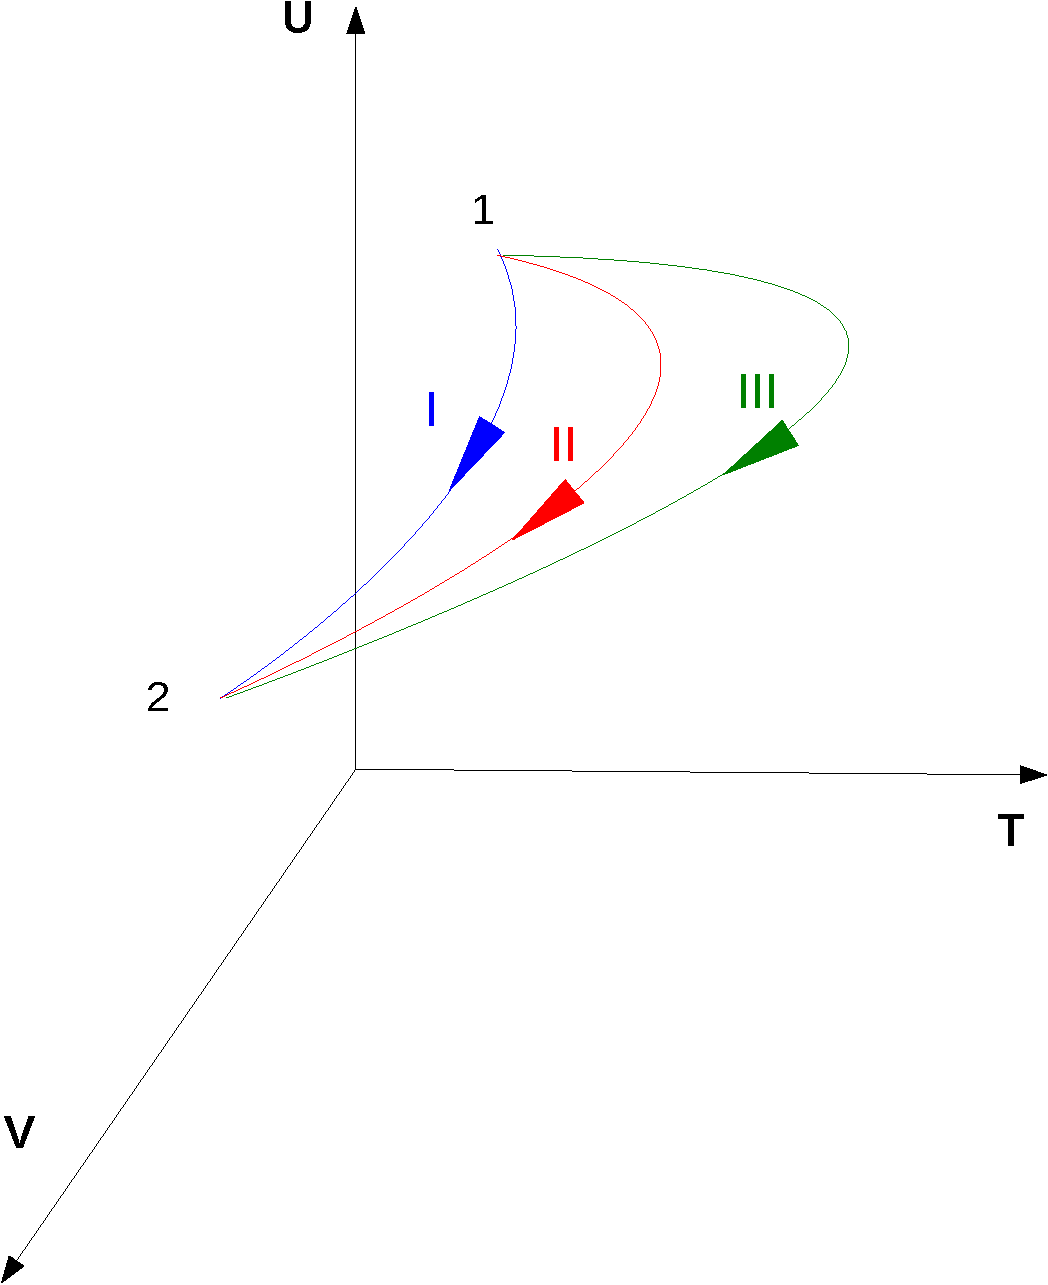
\includegraphics[width=9cm, height=9cm]{./Figs/Chp3_State-PathFunctions}
        \caption{State function: Change of internal function as a result of work and heat being exerted into the system by 3 distinct paths. Note that regardless the chosen path (from state 1 to state 2), $U_{1}$ and $U_{2}$ remain the same, although the amount of heat (represented here by changes in temperature, $T$) and work (\ie changes in volume, $V$) may vary significantly.}\label{Chapter:FirstLaw:Fig:StateFunctions}
     \end{center}
   \end{figure}
   
%%%
%%% SECTION
%%%
   \section{Reversible and Irreversible Processes}\label{Chapter:FirstLaw:Section:Reversibility}\index{Process!Reversible}\index{Process!Irreversible}
   Thermodynamic processes may change the state in two distinct ways:
   \begin{itemize}
     \item {\bf Reversible process} (also known as quasi-static process) is a process which can be stopped at any stage and reversed so that the system and the surroundings are exactly restored to their original states;
     \item {\bf Irreversible process} is a process in which heat is transferred through a finite temperature, thus it is not possible to return both the system and the surroundings to their original states.
   \end{itemize}
   Irreversibilities are of two types:
   \begin{itemize}
      \item {\it external irreversibilities} which are associated with dissipating effects outside the working fluid, \eg mechanical friction during a process due to some external force;
      \item {\it internal irreversibilities} which are associated with dissipating effects within the working fluid, \eg viscosity and inertial of a gas.
   \end{itemize}
   A set of definitions, characteristics and examples of these two processes are given by Table~\ref{Chapter:FirstLaw:TableDiffRevIrrev}. 
   
   
%%%
%%% SECTION
%%%
     \section{The First Law of Thermodynamics}\label{Chapter:FirstLaw:Section:FirstLaw}\index{Laws of Thermodynamics ! First law}
     \begin{subequations}
         Thermal energy is a macro-scale representation of micro-scale changes in mechanical energy (\ie work and heat). In a molecular scale, atoms and molecules are in random motion that can be associated with the kinetic energy of these `particles'. Tracking the motion and energy of each particle is addressed by a field of science called statistical (or quantum) thermodynamics; here we are interested in the consequences of the particles' motion, \ie oscillations in temperature as a measure of the average molecular-scale kinetic energy.
         \begin{shaded}
            \begin{center} {\bf Sign Notation}\end{center} 
              Before we proceed stating the {\it First Law}, we should define a sign notation used for all quantities in this document. Thus any form of energy:
              \begin{itemize}
                  \item Added to the system is assumed \blue{positive}, and;
                  \item Removed from the system is assumed \red{negative}.
              \end{itemize}
              Hence:
              \begin{itemize}
                 \renewcommand{\labelitemi}{$\star$}
                 \item heat added to the system by the neighbourhood is \blue{positive};
                 \item heat removed from the system to the neighbourhood is \red{negative};
                 \item work produced by the system and transferred to the neighbourhood is \red{negative};
                 \item work produced by the neighbourhood and transferred to the system is \blue{positive}.
              \end{itemize}
         \end{shaded}
         In most thermodynamic systems, changes in kinetic and potential energies are often assumed negligible\footnote{Here, we are assuming that such systems are not movable \wrt frames of reference.}, and Eqn.~\ref{Chapter:FirstLaw:Eqn:TotalEnergy3} becomes
            \begin{equation}
               \mfr[E]{2}{cv} - \mfr[E]{1}{cv} = U_{2}-U_{1} = Q_{1-2} + W_{1-2},\label{Chapter:FirstLaw:Eqn:FirstLaw1}
            \end{equation}
         in such cases, the internal energy of a system may be changed in any of the following ways: producing or receiving work and/or have heat being removed or added to the system. Heat and work are equivalent ways of changing the system's internal energy. It was experimentally observed that in isolated systems there is {\bf no} change in the internal energy.

         \begin{shaded}
            The {\it First Law of Thermodynamics} is effectively a statement of energy conservation: `the only way the energy of a closed system can be changed are through transfer of energy by work or heat' \citep{Moran_Book}. In other words: `the internal energy of an isolated system is constant' \citep{Atkins_Book}. Mathematically, these statements can be readily represented in differential form (\ie during infinitesimal changes in the state of the system) by,
            \begin{equation}
               d U = \delta Q + \delta W,\label{Chapter:FirstLaw:Eqn:FirstLaw2}
            \end{equation}
            
         \end{shaded}
   
     \end{subequations}

   %%%
   %%%
   \begin{landscape}
     \begin{table}
       \begin{tabular}{||l | l||}
         \hline\hline
             {\bf Reversible process} (RP)                                    &         {\bf Irreversible process}  (IP)                          \\
         \hline
             (a) RP can not be realised in practice;                          &  (a) All practical processes occurring are IP;                    \\
             (b) The process can be carried out in the reverse direction      &  (b) The process if carries out in reverse direction, it follows  \\
                 following the same path as followed in forward direction;    &      the path different from that in forward direction;           \\
             (c) A RP leaves no trace of occurrence of process upon the       &  (c) The evidences of process having occurred are evident even    \\
                 the system and surroundings after its reversal;              &      after reversal of IP;                                        \\
             (d) Such processes can occur in either directions without        &  (d) Occurrence of IPs in either directions is not possible, as   \\
                 violating the Second Law of Thermodynamics;                  &      in one direction it shall be accompanied with the violation  \\
                                                                              &      of the Second Law of Thermodynamics;                         \\
             (e) A system undergoing RPs has maximum efficiency. Therefore,   &  (e) Systems undergoing IPs do not have maximum efficiency as it  \\
                 sytems with RPs are considered as reference systems (\ie     &      accompanied by waste of energy;                              \\
                 benchmarks);                                                 &                                                                   \\
             (f) RPs occur at infinitesimal rate, \ie quasi-static process;   &  (f) IP occur at finite rate;                                     \\
             (g) System remains in thermodynamic equilibrium during occurrence&  (g) Systems does not remain in thermodynamic equilibrium during  \\
                 of such processes;                                           &      IPs;                                                         \\
         \hline
                                 {\bf Examples}                               &             {\bf Examples}                                        \\
             (h) Frictionless motion, controlled expansion and compression,   &   (h) Viscous fluid flow, inelastic deformation and hysteresis    \\
                 elastic deformations, polytropic expansion and compression   &       effects, free expansion, throttling processes, heat transfer\\
                 of fluids, electrolysis etc.                                 &       combustion, free expansion, diffusion etc.                  \\
         \hline\hline
       \end{tabular}
       \caption{Differences between reversible and irreversible processes \citep[extracted from][]{Singh_Book}.}
       \label{Chapter:FirstLaw:TableDiffRevIrrev}
     \end{table}
   \end{landscape}  
   
   % Example
   \begin{MyExample}{\begin{center}{\bf Example}\end{center}}
     \begin{example}\label{Chapter:FirstLaw:Example1}\citep{Atkins_Book}
        In a power station, the water pump is located in an isolated room. The electric motor of this pump produces 15 kJ of energy as mechanical work and loose 2 kJ of heat to the surroundings. Calculate the change in internal energy of the motor.  
     \end{example}

% SOLUTION
       \noindent{\bf Solution:}
       Here, the system is the electrical motor whereas the surroundings is the room. The work produced by the motor is $\delta W= -15$ kJ and the heat transferred from the engine to the room is $\delta Q = -2$ kJ, therefore 
          \begin{eqnarray}
             dU = \Delta U &=&  \delta Q + \delta W \nonumber \\
                &=& -15 -2 = -17\text{ kJ} \nonumber
          \end{eqnarray}
   \end{MyExample}

   % Example
   \begin{MyExample}{\begin{center}{\bf Example}\end{center}}
     \begin{example}\label{Chapter:FirstLaw:Example2}
       If $P_{1}$ = 3.00 atm, $V_{1}$ = 500 cm$^{3}$, $P_{2}$ = 1.00 atm and $V_{2}$ = 2000 cm$^{3}$. Calculate the work, $W_{\text{rev}}$ (in $J$), for the expansion processes shown in the following figure.
         \begin{center}
           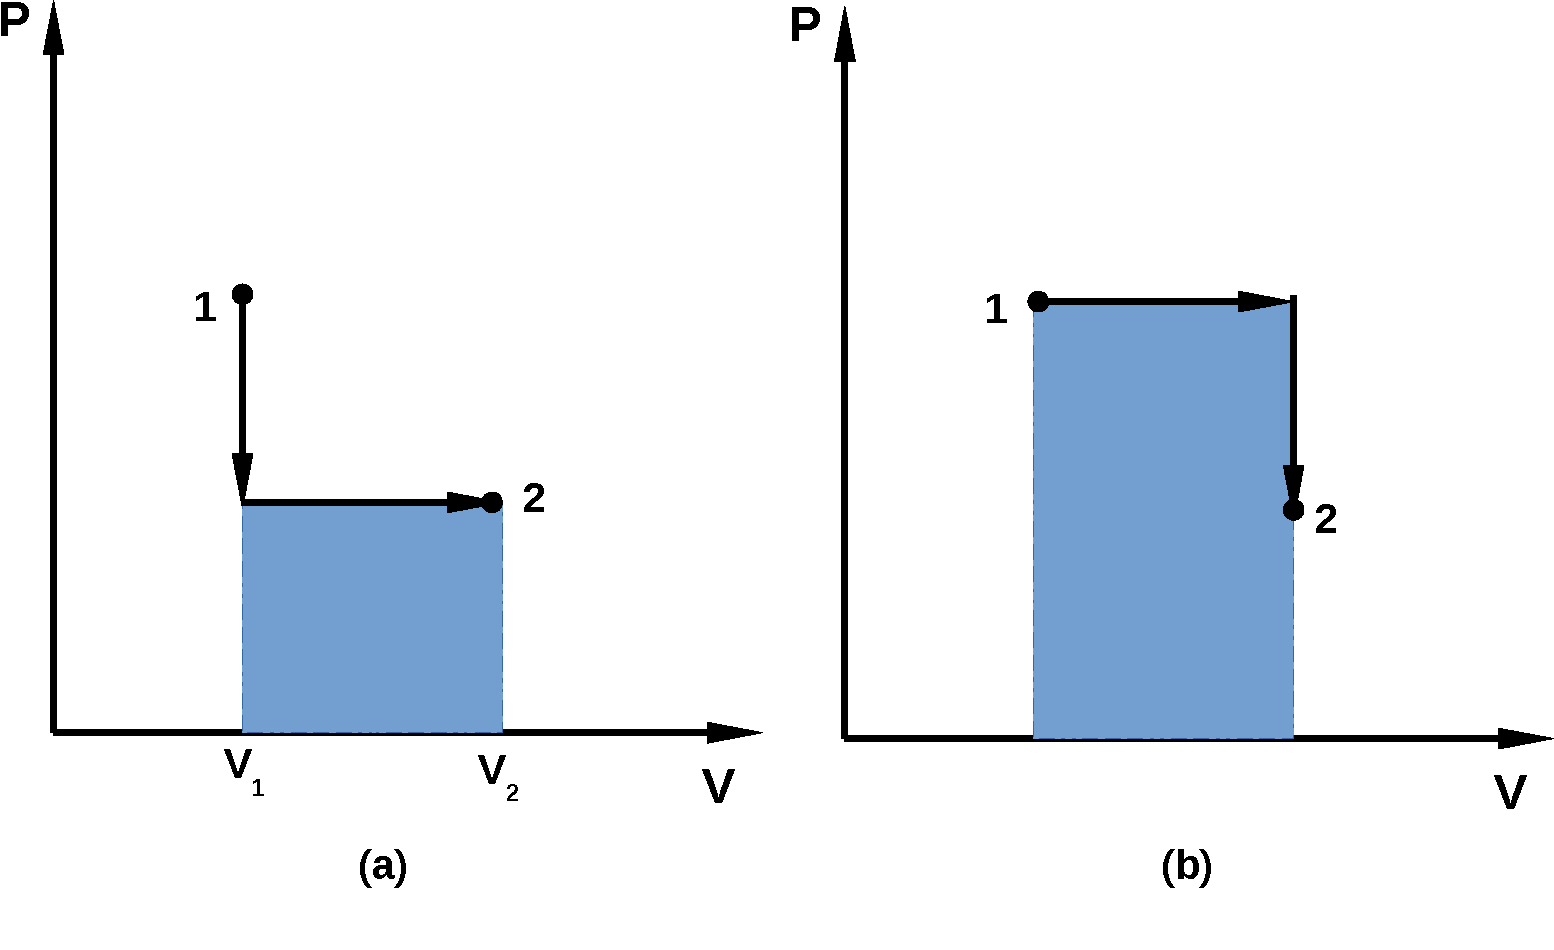
\includegraphics[width=.6\columnwidth,clip]{./Figs/Mod1Ex1}
         \end{center}
     \end{example}
     
% SOLUTION
       \noindent{\bf Solution:} $W_{\text{rev}}$ is related to the area below the curve. Thus, we should use the $PV$ work equation:
           \begin{itemize}
              \item For process {\bf (a)}: 
                 \begin{eqnarray}
                    d W = -PdV \Longrightarrow W &=& -P_{2}\left(V_{2}-V_{1}\right) \nonumber \\
                                                 &=& - 1\text{ atm}\left(2000-500\right)\text{ cm}^{3} = -1500\text{ atm.cm}^{3} \nonumber 
                 \end{eqnarray}
                 Now we need to convert {\it atm.cm}$^{3}$ to $J$, thus using the unit conversion table:
                 \begin{eqnarray}
                     W &=& -1500\blue{\cancel{\text{ atm}}}.\red{\cancel{\text{cm}^{3}}} \frc{1.01325\times 10^{5}\blue{\cancel{\text{ Pa}}}}{1\blue{\cancel{\text{ atm}}}} \frc{1 \frc{\text{kg}}{\text{m.s}^{2}}}{1\blue{\cancel{\text{ Pa}}}} \frc{1\text{ m}^{3}}{ 100^{3} \red{\cancel{\text{ cm}^{3}}}} \nonumber \\
                       &=& -151.9875 \blue{\cancel{\frc{\text{ kg.m}^{2}}{\text{s}^{2}}}} \frc{ 1 \text{ J}}{ \blue{\cancel{\frc{\text{ kg.m}^{2}}{\text{s}^{2}}}}} \nonumber\\
                       &=& -151.9875\text{ J} \nonumber
                 \end{eqnarray}
%
              \item For process {\bf (b)}, since $P$ is constant, i.e., $P_{1}=P_{2}$:
                 \begin{eqnarray}
                    d W = -PdV \Longrightarrow W &=& -P_{1}\left(V_{2}-V_{1}\right) \nonumber \\
                                                 &=& - 3\text{ atm}\left(2000-500\right)\text{ cm}^{3} = -4500\text{ atm.cm}^{3} \nonumber \\
                                                 &=& -455.9625\text{ J} \nonumber
                 \end{eqnarray}
           \end{itemize}
   \end{MyExample}

%%%
%%% SECTION
%%%
     \section{Cycles: Representation of the First Law}\label{Chapter:FirstLaw:Section:FirstLaw_Cycle}\index{Laws of Thermodynamics ! First law}\index{Cycles}
        \begin{subequations}
           \begin{shaded}
               During any cycle, the cyclic integral of heat added to a system is proportional to the cyclic integral of work done by the system.
           \end{shaded}
           This statement clearly indicates that during a cycle the internal energy is zero, $\left(\Delta U\right)_{\text{cycle}}=0$. The mathematical representation of the first law in a cycle is
             \begin{equation}
               \displaystyle\oint \delta Q = -\displaystyle\oint \delta W,\label{Chapter:FirstLaw:Eqn:FirstLawCycle}
             \end{equation}
             where line integral $\left(\oint\right)$ is defined in Appendix~\ref{Appendix_Calculus:Section:LineIntegral}. Two main practical systems arise from the application of the first law to the definition of cycles (Section~\ref{Chapter:Introduction:Section:Introduction:ProcessesCyclesDefinition}): power and refrigeration cycles.
      
%%%% SUBSECTION
          \subsection{Power Cycles}\index{Cycles! Power }
             Power cycles (Fig.~\ref{Chapter:FirstLaw:Fig:PowerRefrigSystems}a) are systems that deliver a net work transfer of energy to the surroundings during each cycle, where
               \begin{displaymath}
                  W_{cycle} = Q_{in} - Q_{out},\;\;\;\text{ with }\;\;\; Q_{in} > Q_{out}.
               \end{displaymath}
             The energy supplied by heat transfer to a system on a power cycle is often derived from combustion processes. Such cycles are used to quantitatively describe the work produced in power plants, and are often assessed through the thermal efficiency of the process,\index{Cycles! Power! Thermal efficiency }
       \begin{equation}
           \eta =\frc{W_{cycle}}{Q_{in}} = \frc{Q_{in} - Q_{out}}{Q_{in}} = 1 - \frc{Q_{out}}{Q_{in}} < 1.\label{Chapter:FirstLaw:Eqn:FirstLawCycle:PowerEfficiency}
       \end{equation}
       For reversible power cycles the ratio of heat transfer, $Q_{cold}/Q_{hot}$ depends only on the reservoirs' temperatures and can be simplified to
       \begin{equation}
          \frc{Q_{\text{cold}}}{Q_{\text{hot}}} =  \frc{T_{\text{cold}}}{T_{\text{hot}}}.\label{Chapter:FirstLaw:Eqn:FirstLawCycle:PowerEfficiency2}
       \end{equation}
       One of the conditions for this expression to be valid is $T_{\text{hot}}\ne0$, indeed {\bf reservoir temperature are always assumed as absolute temperature, \ie expressed in Kelvin}.
       \begin{shaded}
           Thus the thermal efficiency of a reversible power cycle while operating between thermal reservoirs at temperatures $T_{hot}$ and $T_{cold}$ is expressed as
          \begin{equation}
            \eta_{\text{max}} = 1 - \frc{T_{\text{cold}}}{T_{\text{hot}}}\label{Chapter:FirstLaw:Eqn:FirstLawCycle:PowerCarnotEfficiency}
          \end{equation}
          $\eta_{\text{max}}$ is also known as the {\it Carnot efficiency}\index{Carnot Efficiency} and it is the maximum efficiency any power cycle can have while operating between the 2 reservoirs.
       \end{shaded}

   \begin{figure}[h]
      \vbox{
        \hbox{ \hspace{-1.5cm}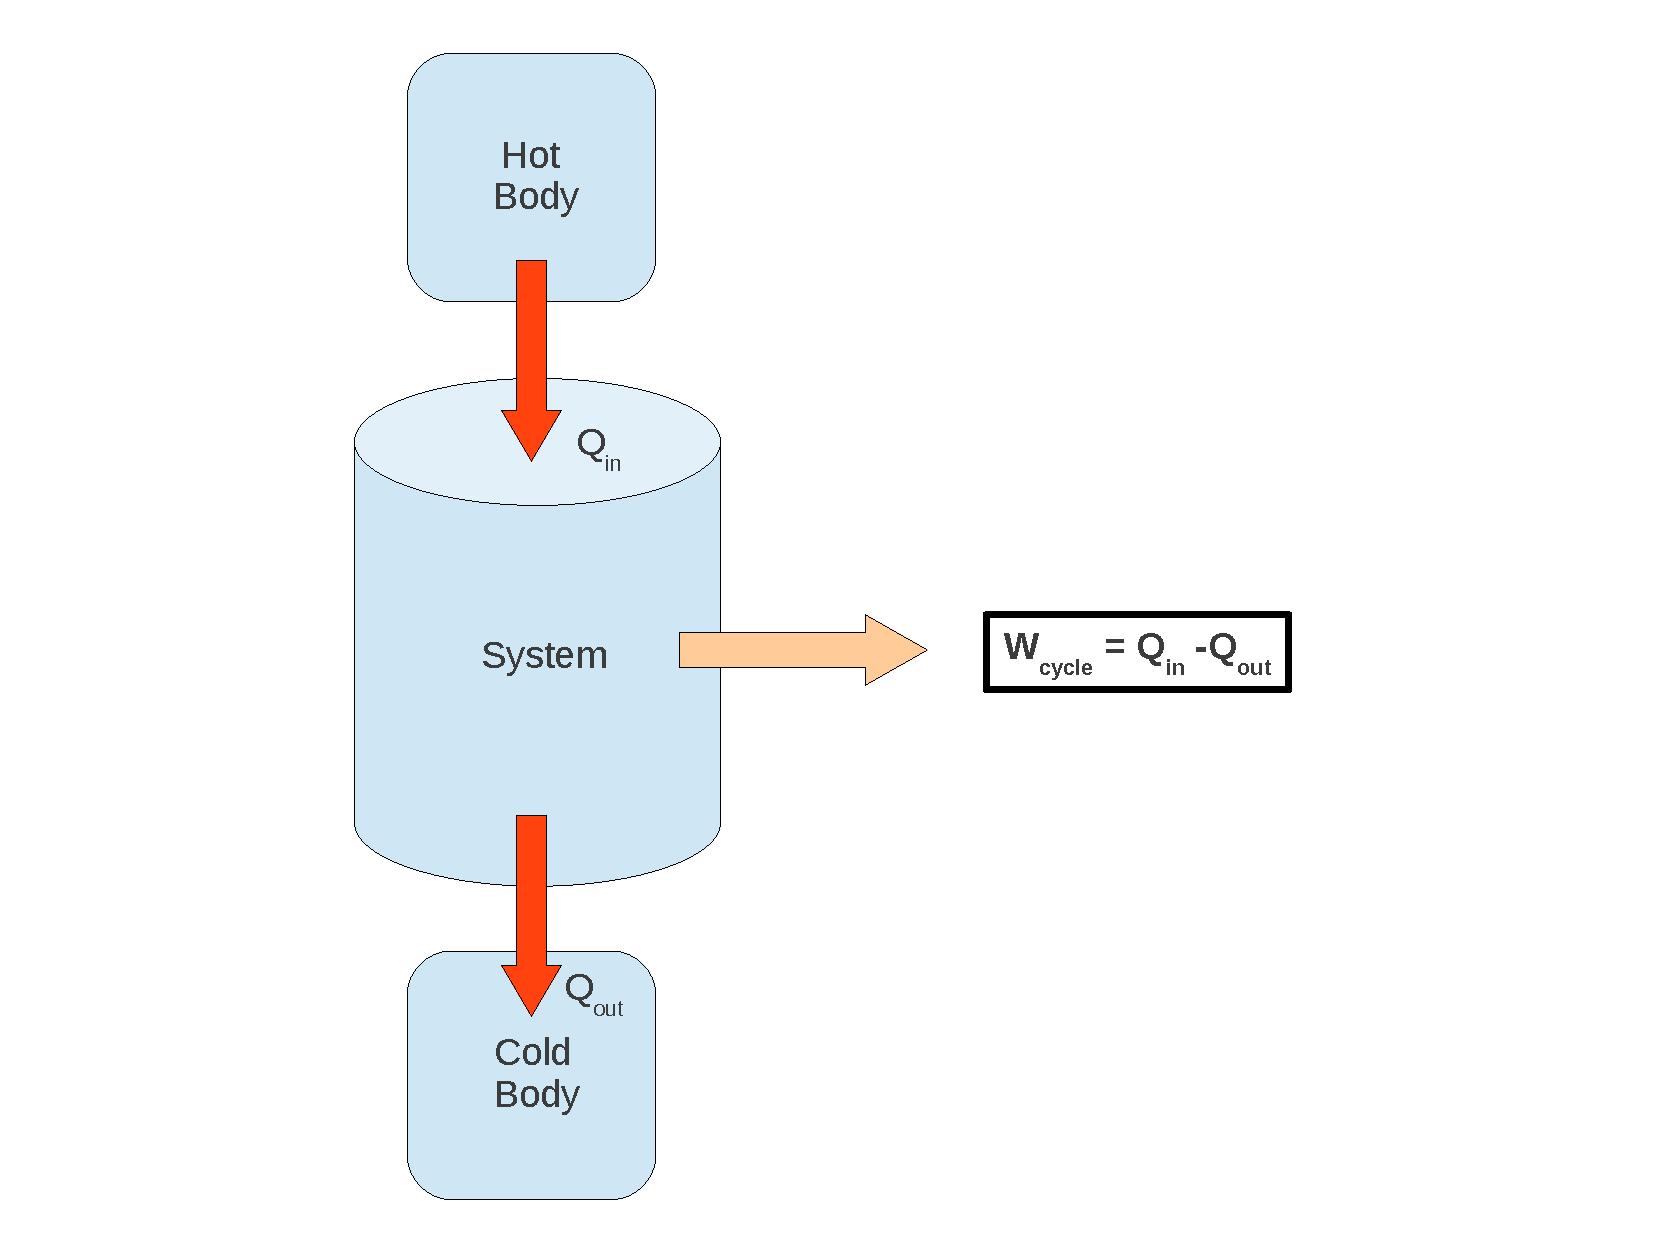
\includegraphics[width=.7\columnwidth,clip]{./Figs/FirstLaw_Cycle_01}
               \hspace{-2.5cm}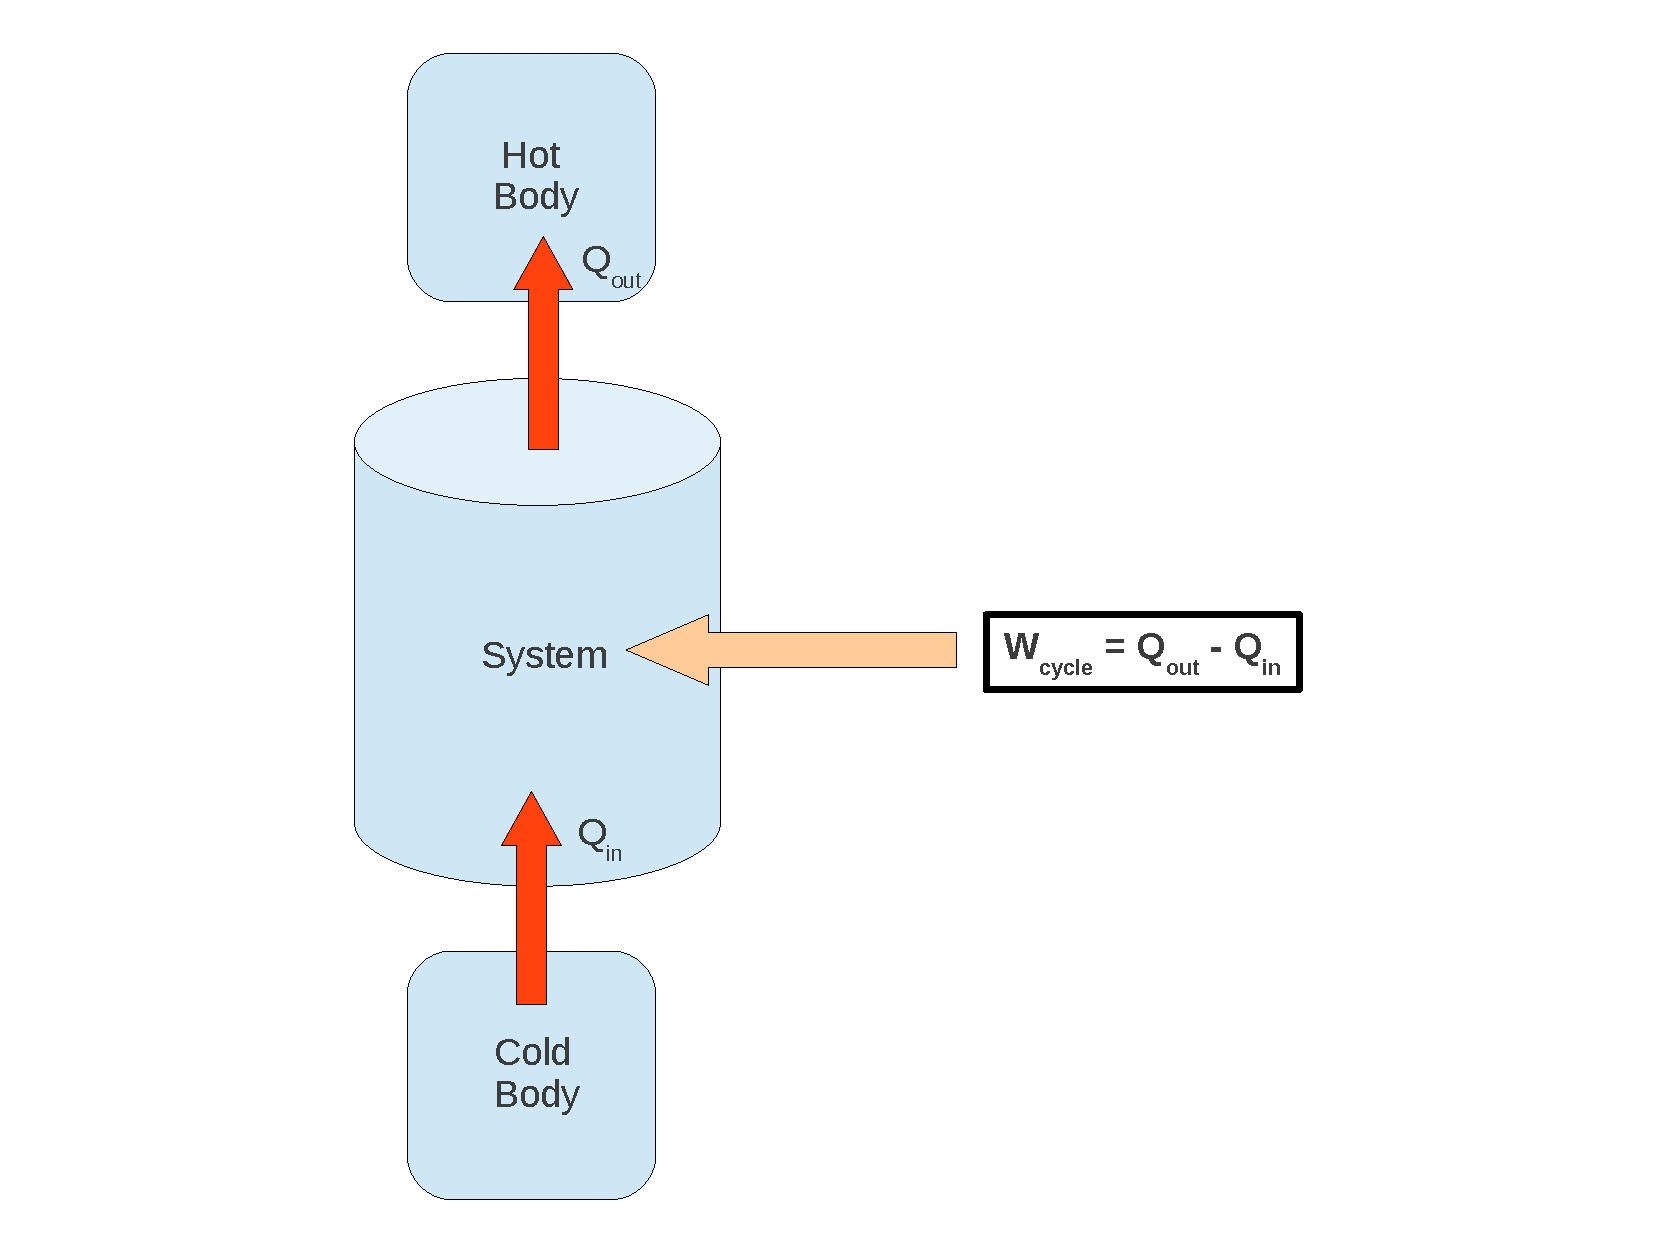
\includegraphics[width=.7\columnwidth,clip]{./Figs/FirstLaw_Cycle_02}}
        \vspace{-0.cm}
        \hbox{\hspace{4cm}(a)\hspace{7cm}(b)}}
       \caption{Schematic representation of (a) power and (b) refrigeration cycles.}\label{Chapter:FirstLaw:Fig:PowerRefrigSystems}
   \end{figure}    

%%%% SUBSECTION
          \subsection{Refrigeration Cycles}\index{Cycles! Refrigeration }
           Refrigeration cycles (Fig.~\ref{Chapter:FirstLaw:Fig:PowerRefrigSystems}b) are systems in which Q$_{in}$ is associated with the heat energy transferred into the system from the cold body. Q$_{out}$ is the energy discharged via heat transfer from the system to the hot body, 
           \begin{displaymath}
              W_{cycle} = Q_{out} - Q_{in}.
           \end{displaymath}
            \begin{shaded}
               The aim of such cycles is to cool a refrigerated body or to maintain the temperature of a body bellow that of the surrounding. Refrigeration cycles are assessed through the coefficient of performance (COP)\index{Cycles!Refrigeration ! Coefficient of performance },
                 \begin{equation}
                   \beta = \frc{Q_{in}}{W_{cycle}} = \frc{Q_{in}}{Q_{out} - Q_{in}}.\label{Chapter:FirstLaw:Eqn:FirstLawCycle:COP}
                 \end{equation}
          \end{shaded}
        \end{subequations}
   

%%%
%%% SECTION
%%%
     \section{Enthalpy}\label{Chapter:FirstLaw:Section:Enthalpy}\index{Enthalpy}
        \begin{subequations}
          Let's consider a gas contained in a piston-cylinder system undergoing a quasi-static isobaric process. Let's also assume that there are no changes in kinetic and potential energies and that the only work done during the process is the one associated with the piston's movement. The first law stated that the internal energy is a result of changes in work and heat,
          \begin{displaymath}
            dU = \delta Q + \delta W,\;\;\;\text{ and } \;\;\; \delta W = -\int\limits_{1}^{2} PdV = -P\left(V_{2}-V_{1}\right).
          \end{displaymath}
          \begin{shaded}
             Replacing the work into the first law equation
             \begin{eqnarray}
                \delta Q &=& dU - \delta W = U_{2} - U_{1} + P_{2}V_{2} - P_{1}V_{1}\nonumber \\
                         &=& \left(U_{2}+P_{2}V_{2}\right) - \left(U_{1}+P_{1}V_{1}\right).\label{Chapter:FirstLaw:Eqn:EnthalpyDefinition1}
             \end{eqnarray}
             The terms in brackets, $U+PV$, are thermodynamic properties that depend only on the state of the system and, as such, define a new extensive property, the {\it enthalpy},
             \begin{equation}
               H\equiv U + PV.\label{Chapter:FirstLaw:Eqn:EnthalpyDefinition2}
             \end{equation}
             Replacing Eqn.~\ref{Chapter:FirstLaw:Eqn:EnthalpyDefinition1} in \ref{Chapter:FirstLaw:Eqn:EnthalpyDefinition2}
             \begin{equation}
               \delta Q = \overbrace{\left(U_{2}+P_{2}V_{2}\right)}^{H_{2}} - \overbrace{\left(U_{1}+P_{1}V_{1}\right)}^{H_{1}} = H_{2}-H_{1} = \Delta H,\label{Chapter:FirstLaw:Eqn:EnthalpyDefinition3}
             \end{equation}
             \ie the {\it change in enthalpy leads to the heat transfer for isobaric processes}. 
          \end{shaded}
       
        \end{subequations}

%%%
%%% SECTION
%%%
    \section{Heat Capacities}\label{Chapter:FirstLaw:Section:HeatCapacity}
      \begin{subequations}

        %%% Subsection
        \subsection{Constant Volume and Constant Pressure Heat Capacities}\index{Heat Capacity ! Constant Volume}\index{Heat Capacity ! Constant Pressure}\index{$C_{v}$| see{ Heat Capacity}}\index{$C_{p}$| see{ Heat Capacity}}
            {\it Specific heat capacity} can be defined as the amount of heat necessary to increase the temperature of a unit mass of material by one degree. Mathematically, it can be defined as
            \begin{displaymath}
              C\equiv \frc{1}{m}\frc{\delta Q}{\delta T}.
            \end{displaymath}
            As $Q$ is path-dependent, $C$ also is, and from the first law
            \begin{displaymath}
              \delta Q = dU - \delta W \;\;\Longrightarrow\;\; dU + PdV,
            \end{displaymath}
            two properties can be defined depending upon the path:
            \begin{enumerate}[(i)]
              \item Constant volume: in which the term $PdV$ vanishes and the specific heat at constant volume $\left(C_{v}\right)$ is
                \begin{equation}
                  C_{v} = \frc{1}{m}\left(\frc{\delta Q}{\delta T}\right)_{V} = \frc{1}{m}\left(\frc{\partial U}{\partial T}\right)_{V} = \left(\frc{\partial u}{\partial T}\right)_{V}\label{Chapter:FirstLaw:Eqn:HeatCapacityConstVolume1}
                \end{equation}
              \item Constant pressure: in which the work term can be integrated at constant pressure, hence the heat transfer can be expressed in terms of the enthalpy change (Eqn.~\ref{Chapter:FirstLaw:Eqn:EnthalpyDefinition3}),
                \begin{equation}
                  C_{p} = \frc{1}{m}\left(\frc{\delta Q}{\delta T}\right)_{P} = \frc{1}{m}\left(\frc{\partial H}{\partial T}\right)_{P} = \left(\frc{\partial h}{\partial T}\right)_{P}\label{Chapter:FirstLaw:Eqn:HeatCapacityConstPressure1}
                \end{equation}
            \end{enumerate}
            $C_{p}\left(T,P\right)$ and $C_{v}\left(T,v\right)$ are thermodynamic properties for general materials and can vary with the independent variables $\left(T, P, v\right)$. Here, $h$ and $u$ are specific enthalpy and internal energy with units J.kg$^{-1}$.
            
        %%% Subsection
        \subsection{Heat Capacity Relations for Ideal Gases}\label{Chapter:FirstLaw:Section:HeatCapacity:IdealGas}
          For ideal gases, one can use the fundamental thermodynamic relation that defined enthalpy (Eqn.~\ref{Chapter:FirstLaw:Eqn:EnthalpyDefinition2}) and the ideal gas EOS, $Pv=RT$ (Eqn.~\ref{Chapter:Intro_Property_of_Gases:Eqn:IdealEOS}), to redefine the specific enthalpy
          \begin{equation}
            h = u(T) + RT,\label{Chapter:FirstLaw:Eqn:EnthalpyDefinition4}
          \end{equation}
          of an ideal gas as a function of $T$ only, \ie $h=h(T)$.  The specific heat of an ideal gas at contant volume is expressed as
          \begin{displaymath}
             C_{v}(T,v) = \left(\frc{\partial u}{\partial T}\right)_{v} = \frc{d}{dT}\left(u(T)\right) = C_{v}(T).
          \end{displaymath}
          In other words, $C_{v}$ is property that can be expressed as function of $T$ and $v$ (thus being defined as a partial differential equation with the differential operator $\partial$), however if a process is assumed isochoric (\ie constant volume) this property becomes a function of only the temperature (and therefore defined as an ordinary differential equation with the differential operator $d$),
                \begin{equation}
                  du = C_{v}(T)dT.\label{Chapter:FirstLaw:Eqn:HeatCapacityConstVolume2}
                \end{equation}
          A similar argument can be used for $C_{p}$ in isobaric processes, leading to
                \begin{equation}
                  dh = C_{p}(T)dT.\label{Chapter:FirstLaw:Eqn:HeatCapacityConstPressure2}
                \end{equation}
          \begin{shaded}
             Differentiating Eqn.~\ref{Chapter:FirstLaw:Eqn:EnthalpyDefinition4} and replacing $du$ and $dh$,
                \begin{eqnarray}
                   && dh = du + RdT \nonumber \\
                   && C_{p}(T)dT = C_{v}(T)dT + RdT \;\;\;\Longrightarrow C_{p}(T) = C_{v} + R \nonumber \\
                   && C_{p}(T) - C_{v}(T) = R.\label{Chapter:FirstLaw:Eqn:HeatCapacitiesRelation_IdealGas1}
                \end{eqnarray}
             A useful relationship in engineering thermodynamics is the ratio of specific heats (or isentropic index),
                \begin{equation}
                  \gamma = \frc{C_{p}}{C_{v}},\label{Chapter:FirstLaw:Eqn:HeatCapacitiesRelation1}
                \end{equation}
             which is valid for any material. For an ideal gas, this relation reduces to 
                \begin{equation}
                  \gamma = \frc{C_{v}(T)+R}{C_{v}(T)} = 1 + \frc{R}{C_{v}(T)}.\label{Chapter:FirstLaw:Eqn:HeatCapacitiesRelation_IdealGas2}
                \end{equation}
             Other heat capacity based relations for ideal gases can be obtained from Eqns.~\ref{Chapter:FirstLaw:Eqn:FirstLaw2}, \ref{Chapter:FirstLaw:Eqn:EnthalpyDefinition2} and \ref{Chapter:Intro_Property_of_Gases:Eqn:IdealEOS}:
                \begin{equation}
                   \delta Q = 
                      \begin{cases}
                         C_{p}dT - \frc{RT}{P}dP, \label{Chapter:FirstLaw:Eqn:HeatCapacitiesRelation_IdealGas3} \\
                         \frc{C_{p}}{R}PdV + \frc{C_{v}}{R}VdP.
                      \end{cases}
                \end{equation}
                These relations, although apparently simple, reveal the dependence of heat transfer on temperature, pressure and volume in processes involving ideal gases.
          \end{shaded}


        \end{subequations}


   % Example
   \begin{MyExample}{\begin{center}{\bf Example}\end{center}}
     \begin{example}\label{Chapter:FirstLaw:Example3}
       Calculate the internal energy (in $J$) when 1 mol of water is isobarically heated from 25$^{\circ}$C to 30$^{\circ}$C at 1 atm. Given: densities of water are 0.9970 g.cm$^{-3}$ at 0$^{\circ}$C and 0.9956 g.cm$^{-3}$ at 100$^{\circ}$C. Molar mass and heat capacity at constant pressure of water are 18 g.mol$^{-1}$ and 1 cal.$\left(\text{g.}^{\circ}\text{C}\right)^{-1}$, respectively.
     \end{example}
     
% SOLUTION
       \noindent{\bf Solution:} From the 1$^{\text{st}}$ Law, $U=Q+W$ ,and in order to calculate $U$ we first need to obtain heat ($Q$) and work ($W$). $Q$ can be obtained from the heat capacity equation
          \begin{displaymath}
             Q = m C_{p} \Delta T,
          \end{displaymath}  
          where $m$ is the mass of water can be obtained from
          \begin{displaymath}
             n = \frc{m}{MW} \Longrightarrow  m = n.MW = 1\text{ mol} . 18 \frc{\text{g}}{\text{mol}} = 18 \text{ g}
          \end{displaymath}
          $n$ and $MW$ are number of moles and molar mass, respectively. Now,
          \begin{displaymath}
             Q = m C_{p} \Delta T = 18\text{ g} . 1 \frc{\text{ cal}}{\text{g.}^{\circ}\text{C}}.\left(30-25\right)^{\circ}\text{C} = 90\text{ cal}
          \end{displaymath}  
          Now, we should calculate the work through $W=-P\Delta V$, however $V$ is not known, but we can obtain it from the density relation $V=m/\rho$, thus
          \begin{displaymath}
             W = - P\Delta V = -P\left(V_{2}-V_{1}\right) = -P\left(\frc{m}{\rho_{2}} - \frc{m}{\rho_{1}}\right) = -0.025\text{atm.cm}^{3} = -0.0006\text{ cal} 
          \end{displaymath}
          Now, calculating the internal energy,
          \begin{displaymath}
             U = Q + W = 89.9994\cancel{\text{ cal}} . \frc{ 4.186\text{ J}}{1\cancel{\text{ cal}}} = 376.7375 \text{ J}
          \end{displaymath}
   \end{MyExample}


   % Example
   \begin{MyExample}{\begin{center}{\bf Example}\end{center}}
     \begin{example}\label{Chapter:FirstLaw:Example4}\citep{Rajput_Book}
       A 0.3 m$^{3}$  tank contains oxygen initially at 100 kPa and 300 K. A paddle wheel within the tank is rotated until the pressure inside rise to 150 kPa. During the process 2 kJ of heat is lost to the surroundings. Determine the paddle-wheel work done (in kJ). Neglect the energy stored in the paddle wheel and assume the heat capacity at constant volume of oxygen is 0.6745 kJ.$\left(\text{kg.K}\right)^{1}$. Given molar mass of oxygen of 32 g.mol$^{-1}$.
     \end{example}
     
% SOLUTION
       \noindent{\bf Solution:} The volume of the tank remains constant $V_{2}=V_{1}=V=$ 0.3 m$^{3}$ during the whole process. Thus, we can define:
            \begin{center}
              \begin{tabular}{l l l l}
                 Initial Condition & $P_{1}=$ 100 kPa   & $T_{1}=$ 300 K         & $V_{1}=$ 0.3 m$^{3}$  \\
                 Final Condition   & $P_{2}=$ 150 kPa   &                       & $V_{2}=$ 0.3 m$^{3}$ \\
                 Heat Loss         & $Q=$ -2 kJ        &                       &                    
              \end{tabular}
            \end{center}
       The compression occurs in a closed system (i.e., constant mass) and, as there is no further information, we may consider that oxygen behaves as an ideal gas. The work added to the system by the paddle can be expressed by $U=Q+W$. Our first step is to calculate $T_{2}$,
       \begin{displaymath}
          \frc{P V}{T} = \text{ constant} \Rightarrow \frc{P_{1}V_{1}}{T_{1}} = \frc{P_{2}V_{2}}{T_{2}} \Rightarrow \frc{P_{1}}{T_{1}}=\frc{P_{2}}{T_{2}} \Rightarrow T_{2} = 450\text{ K}
       \end{displaymath}
        The specific internal energy can defined by the fundamental relation, $du=C_{v}dT$ (check the units for this relation!), where $C_{v}$ is the heat capacity at constant volume thus,
       \begin{displaymath}
          \Delta U = m\Delta u = C_{v}\Delta T = Q + W,
       \end{displaymath}
       therefore, we need to obtain the mass of oxygen in the tank through the ideal gas equation of state,
       \begin{eqnarray}
         P V = n R T \Rightarrow n = \frc{m}{MW} = \frc{P V}{R T} \Rightarrow m &=& \frc{ MW P V}{R T} \nonumber \\
                                                      &=& \frc{ 32\frc{\text{ g}}{\text{mol}} 100\text{ kPa} . 0.3\text{ m}^{3}}{ 8.3143 \frc{\text{J}}{\text{mol.K}} 300\text{ K}} \nonumber \\
                                                      &=& 0.3848 \frc{\text{ g.kPa.m}^{3}}{\text{J}} \frc{1 \text{ J}}{1\text{ N.m}} \frc{1000 \text{ Pa}}{1 \text{ kPa}} \frc{ 1 \text{ N.m}^{-2}}{1\text{ Pa}} \nonumber\\
                                                      &=& 0.3848\text{ kg}\nonumber
       \end{eqnarray}
       Thus
       \begin{eqnarray}
          \Delta u = m C_{v}\Delta T = Q + W \Rightarrow W &=& m C_{v}\left(T_{2}-T_{1}\right) - Q \nonumber \\
                                                          &=& 0.3848\text{ kg} \times 0.6745 \frc{\text{kJ}}{\text{kg.K}}\times (450-300)\text{ K} - (-2 \text{ kJ}) \nonumber \\
                                                          &=& 40.9321\text{ kJ}. \nonumber
       \end{eqnarray}
       The paddle-wheel executed 40.9321 kJ of work to the system.
   \end{MyExample}
   
   % Example
   \begin{MyExample}{\begin{center}{\bf Example}\end{center}}
     \begin{example}\label{Chapter:FirstLaw:Example4}\citep{Atkins_Book}
       Calculate the change in molar enthalpy of N $_{2}$(g) when it is heated from 25$^{\circ}$C to 100$^{\circ}$C. The heat capacity is given by
       \begin{displaymath}
         C_{p} = a + bT + \frc{c}{T^{2}}, 
       \end{displaymath}
       where $\left[C_{p}\right]=$ J.mol$^{-1}$.K$^{-1}$, $\left[T\right]=$ K, $a=$ = 28.58 J.mol$^{-1}$.K$^{-1}$, $b=$ 3.77$\times$10$^{-3}$ J.mol$^{-1}$ and $c=$ -0.50$\times$10$^{5}$ J.mol$^{-1}$.K. Given molar enthalpy of N $_{2}$(g) at 25$^{\circ}$C is 29.1400 J.mol$^{-1}$.
     \end{example}
     
% SOLUTION
     \noindent{\bf Solution:} As all units contain temperature in Kelvin, let's first convert them as $T_{1}=$ 298.15 K and $T_{2}=$ 373.15 K. Now, we need to calculate the change in molar enthalpy in this temperature range using the definition of heat capacity,
        \begin{eqnarray}
          && C_{p} = \left(\frc{\partial H}{\partial T}\right)_{P} \;\;\Longrightarrow\;\; dH = C_{p}dT \nonumber \\
          && \int\limits_{H_{1}\left(T_{1}\right)}^{H_{2}\left(T_{2}\right)}dH = \int\limits_{T_{1}}^{T_{2}} C_{p}dT = \int\limits_{T_{1}}^{T_{2}} \left(a + bT + \frc{c}{T^{2}}\right)dT \nonumber \\
          && H_{2}\left(T_{2}\right) - H_{1}\left(T_{1}\right) = a\left(T_{2}-T_{1}\right) + \frc{1}{2}b\left(T_{2}^{2}-T_{1}^{2}\right) - c\left(\frc{1}{T_{2}}-\frc{1}{T_{1}}\right) \nonumber 
        \end{eqnarray}
        Solving this expression with the constants and $H_{1}\left(T_{1}\right)=H\left(\text{298.15 K}\right)=$ 29.14 J.mol$^{-1}$, leads to $H_{2}\left(T_{2}\right) = H\left(\text{373.15 K}\right)=$ 2238.4047 J.mol$^{-1}$. Thus, change in molar enthalpy, \ie $H_{2}\left(T_{2}\right) - H_{1}\left(T_{1}\right)$,  of N $_{2}$(g) is 2209.2647 J.mol$^{-1}$.

   \end{MyExample} 
       
      
%%%
%%% SECTION
%%%
     \section{Work Done at Moving Boundary}\label{Chapter:FirstLaw:Section:Work}
     \begin{subequations}
        In Section~\ref{Chapter:Introduction:Section:ThermodynamicWorkHeat}, the work produced by (or exerted on) the system was defined by Eqn.~\ref{Chpt01_Work2},
           \begin{equation}
              dW = -PdV \;\;\Longrightarrow \;\; W = - \int\limits_{V_{1}}^{V_{2}} PdV,\label{Chapter:FirstLaw:Eqn:Work1}
           \end{equation}
        where $P$ is the pressure and $V$ is the variable volume. Let's consider a system comprising a cylinder containing a compressible gas $\left(\text{with }V_{1}\text{ and } P_{g} = P_{1}\right)$ with a movable piston (Fig.~\ref{Chapter:FirstLaw:Fig:Work1}). An external pressure $\left(P_{\text{ext}} > P_{1}\right)$ is imposed on the piston and continuously compress the gas until the pressures are equalised $\left(P_{\text{ext}} = P_{g} = P_{2}\right)$. At the end of such compression (\ie at state 2) $V_{2}<V_{1}$ and the work $W$ is positive, \ie energy is transferred to the system through the application of an external force. Now, let's assume that at state 2, $P_{\text{ext}}$ is replaced by a new pressure, $P^{\star}_{\text{ext}}=P_{1}$, such that $P^{\star}_{\text{ext}} < P_{\text{ext}} \left(= P_{g} = P_{2}\right)$. As the new pressure is smaller than the pressure inside the cylinder $\left(P_{2}\right)$, the gas will expand until the external and internal pressure are equal, \ie $P_{g} = P^{\star}_{\text{ext}} = P_{1}$. At the end of such expansion from $V_{2}$ to $V_{1}$, the work
           \begin{displaymath}
              W = - \int\limits_{V_{2}}^{V_{1}} PdV,
           \end{displaymath}
           is negative, \ie energy is transferred from the system to the neighbourhood. In these expansion and compression processes, two scenarios may occur: constant or variable pressures. Equation~\ref{Chapter:FirstLaw:Eqn:Work1} is solved according with these scenarios.
\medskip
% Figure
   \begin{figure}[h]
     \begin{center}
        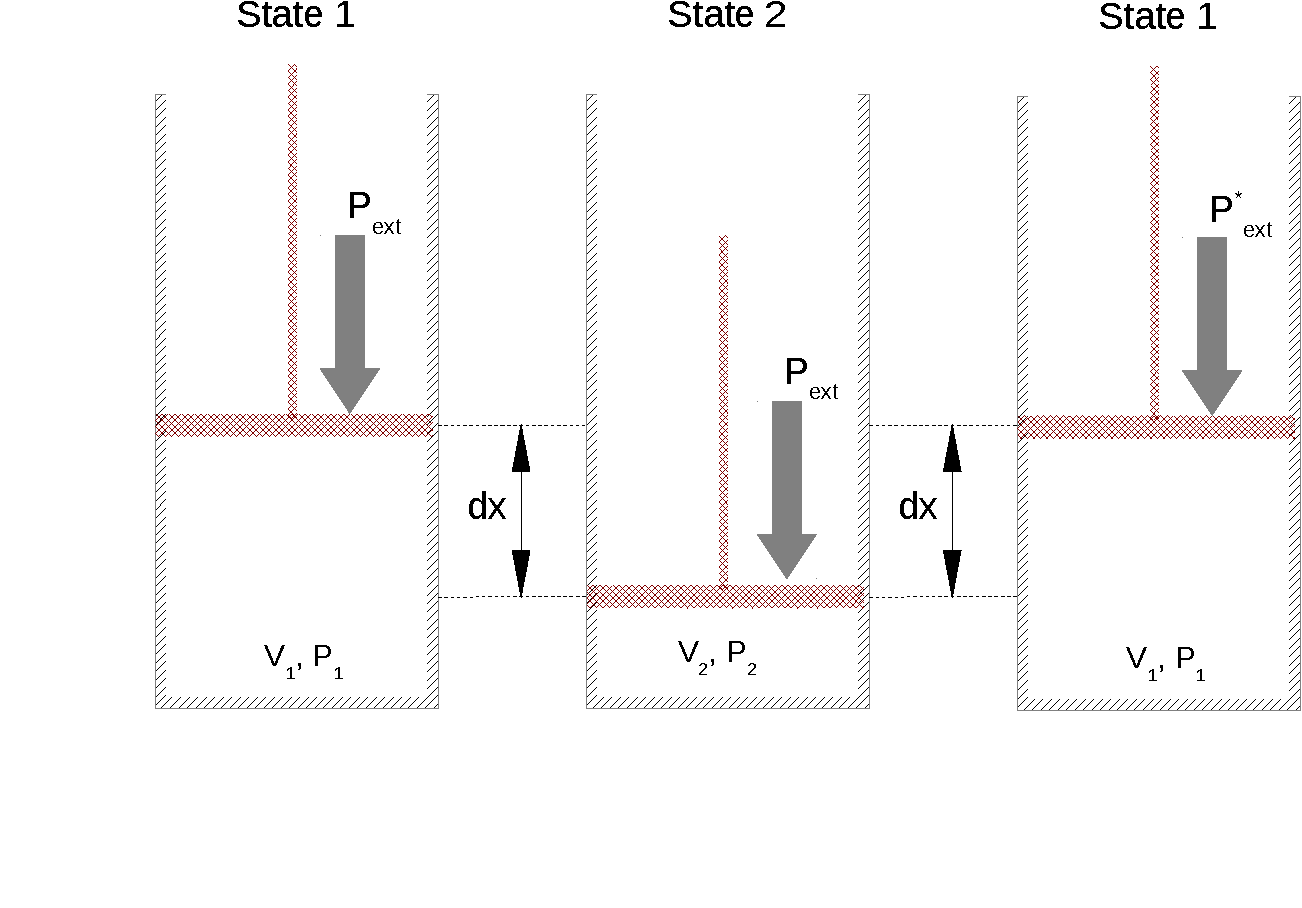
\includegraphics[width=0.7\columnwidth,clip]{./Figs/Chp3_PistonCylinder1}\vspace{-2cm}
        \caption{Compression and expansion of a piston as a result of an external force.}\label{Chapter:FirstLaw:Fig:Work1}
     \end{center}
   \end{figure}
\medskip


%%%
%%% SECTION
%%%
     \subsection{Expansion/Compression under Constant Pressure}\label{Chapter:FirstLaw:Section:Work_ConstantPressure}
        If the external pressure $P=P_{\text{ext}}$ is constant, the integral (Eqn.~\ref{Chapter:FirstLaw:Eqn:Work1}) can be readily solved with the initial and final volumes,
           \begin{shaded}
             \begin{equation}
                dW = -PdV \;\;\Longrightarrow \;\; W = - P\int\limits_{V_{1}}^{V_{2}} dV = - P\left(V_{2}-V_{1}\right) = -P\Delta V.\label{Chapter:FirstLaw:Eqn:Work_ConstPressure}
             \end{equation}
           \end{shaded}
           This integral can be graphically illustrated by the area under the $PV$ curve of Fig.~\ref{Chapter:FirstLaw:Fig:Work2}a. The work is equal to area beneath the horizontal line at $P=P_{\text{ext}}$ lying between $V_{1}$ and $V_{2}$.
           
% Figure
\begin{figure}[h]
  \vbox{
     \hbox{\hspace{2cm}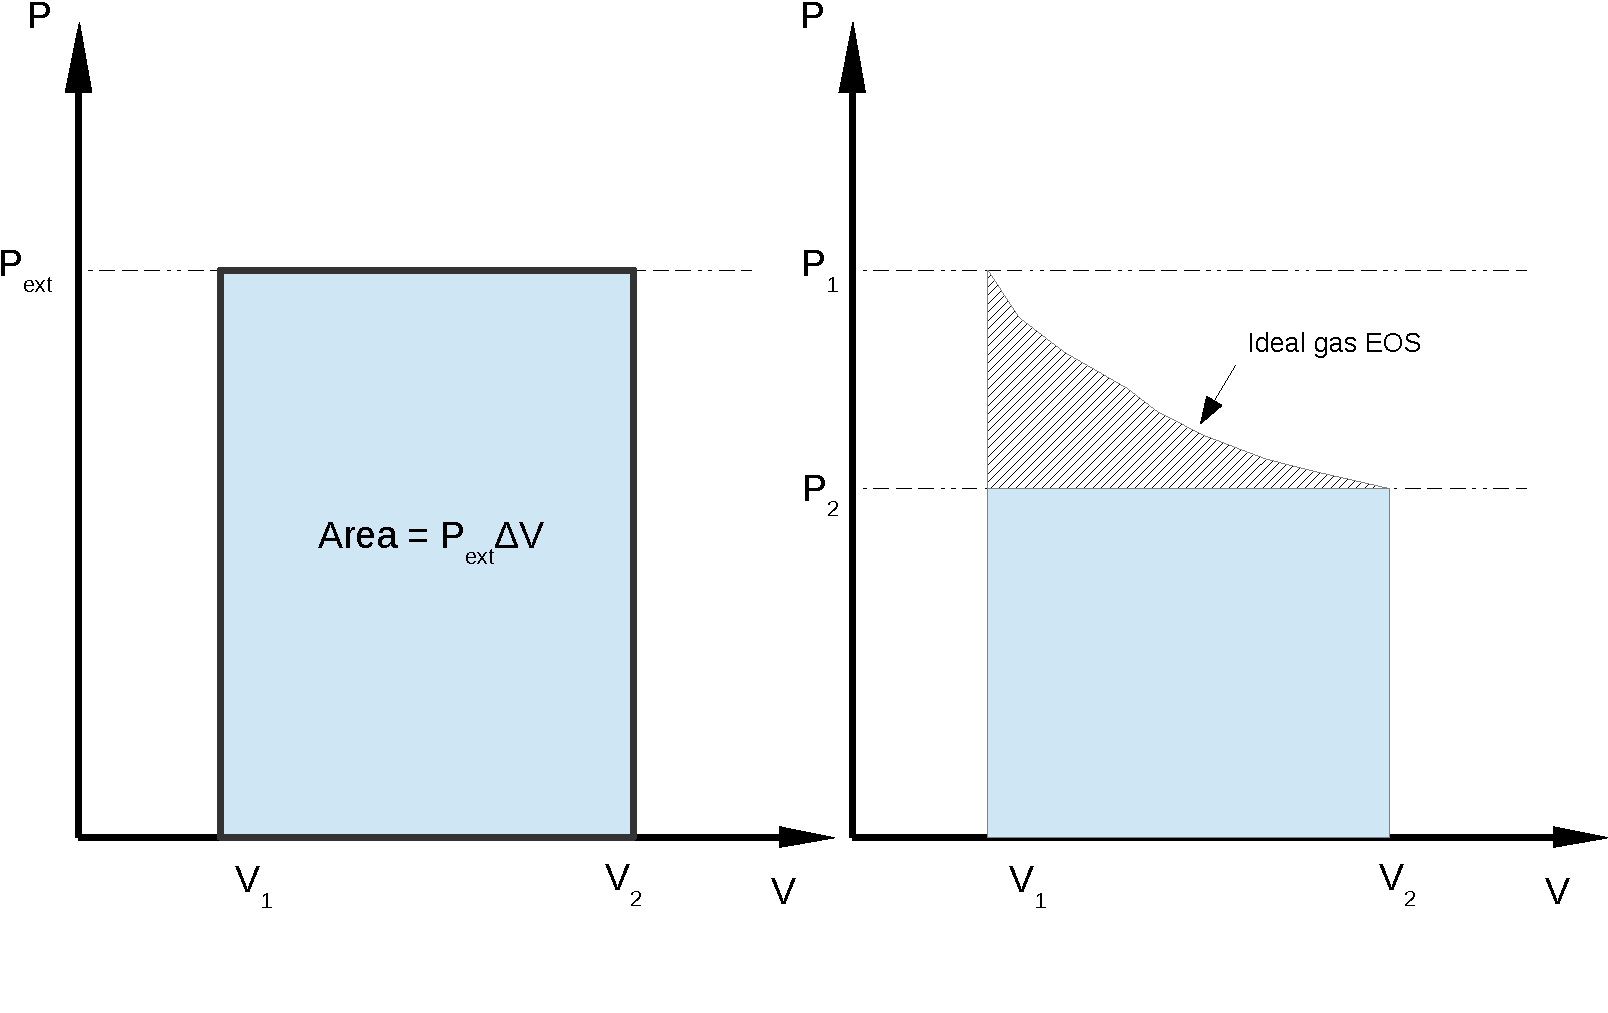
\includegraphics[width=0.7\columnwidth,clip]{./Figs/Chp3_PistonCylinder2}}
     \vspace{-1.cm}
     \hbox{\hspace{5cm}(a)\hspace{4.5cm}(b)}}%\vspace{-0.cm}
        \caption{Ideal gas expansion under isothermal conditions: (a) irreversible work at constant external pressure is equal to the blue area (Eqn.~\ref{Chapter:FirstLaw:Eqn:Work_ConstPressure}); (b) reversible work from $V_{1}$ to $V_{2}$ is given by the area below the curve (\ie blue and hatched areas).}\label{Chapter:FirstLaw:Fig:Work2}
   \end{figure}

%%%
%%% SECTION
%%%
     \subsection{Reversible Expansion}\label{Chapter:FirstLaw:Section:Work_ReversibleExpansion}
     In reversible processes, changes in the state can be reversed by infinitesimal modification of relevant properties. Let's suppose a gas confined in the piston-cylinder system (Fig.~\ref{Chapter:FirstLaw:Fig:Work1}) at stage 2. If the external pressure, $P_{\text{ext}}$ is set equal to the gas pressure, $P_{2}$, thus there is no movement of the piston as the system is in mechanical equilibrium with the surroundings. Any infinitesimal change in $P_{\text{ext}}$ leads to changes in volume, \ie an infinitesimal reduction in the external pressure results in slight expansion of the gas (increase of the volume), whereas an infinitesimal increase of the external pressure leads to slight gas contraction (decrease of the volume).

     In both scenarios, the change is reversible, however if the external pressure differs measurably from the internal (gas) pressure, then changing $P_{\text{ext}}$ infinitesimally will not change the volume of the gas (\ie the direction of the piston movement). Such a system is not in mechanical equilibrium with its surroundings and the expansion/contraction is thermodynamically irreversible.

     For reversible expansion, $P_{\text{ext}}$ is assumed to be equal to $P$ (internal gas pressure) at each stage of the expansion, $P_{\text{ext}}=P$,
           \begin{shaded}
             \begin{equation}
                dW_{\text{rev}} = -P_{\text{ext}}dV = -PdV \;\;\Longrightarrow \;\; W_{\text{rev}} = -\int\limits_{V_{1}}^{V_{2}}PdV.\label{Chapter:FirstLaw:Eqn:Work_ReversibleExpansion}
             \end{equation}
             The integral can only be evaluated once the behaviour of the confined pressure is known and can be expressed by an algebraic equation as a function of the volume.
           \end{shaded}

           \begin{MyBlock}{Isothermal Reversible Expansion}
             Let's suppose a scenario in which an ideal gas undergoes an isothermal reversible expansion. In such scenario, the system (\eg piston-cylinder) remains in thermal equilibrium with its surrounding at a prescribed and constant temperature (\eg a constant temperature bath). In this case, $T$, $R$ and $n$ (closed system) are constants and may be taken outside the integral (Eqn.~\ref{Chapter:FirstLaw:Eqn:Work_ReversibleExpansion}), and the integral from $V_{1}$ to $V_{2}$ becomes,
             \begin{equation}
               W_{\text{rev}} = -\int\limits_{V_{1}}^{V_{2}}PdV = -n R T\int\limits_{V_{1}}^{V_{2}}\frc{dV}{V} = -n R T\ln{\frc{V_{2}}{V_{1}}}.\label{Chapter:FirstLaw:Eqn:Work_IsothermalReversibleExpansion}
             \end{equation}
             If the final volume is larger than the initial volume $\left(V_{2} > V_{1}\right)$ (as in any expansion), the logarithm term in Eqn.~\ref{Chapter:FirstLaw:Eqn:Work_IsothermalReversibleExpansion} is positive, thus $W_{\text{rev}}$ is negative, \ie, the system has produced work. Similarly, if the gas undergoes a compression $\left(\text{and therefore } V_{2} < V_{1}\right)$, thus $W_{\text{rev}}$ is positive as the logarithm term is negative.

             The work produced during the isothermal reversible expansion of an ideal gas is graphically represented in Fig.~\ref{Chapter:FirstLaw:Fig:Work2}b. Reversible work (integral $PdV$) is the (blue + hatched) area under the ideal gas EOS curve from $V_{1}$ to $V_{2}$, whereas the area in blue is effectively the irreversible work at a constant external pressure $P_{\text{ext}} = P_{2}$. Such graphical representation shows that reversible work is larger than the corresponding irreversible work of a similar system.
           \end{MyBlock}


   % Example
   \begin{MyExample}{\begin{center}{\bf Example}\end{center}}
     \begin{example}\label{Chapter:FirstLaw:Example6}\citep{Rajput_Book}
       A gas contained in a piston-cylinder system undergoes a reversible compression from 1.5 to 7.5 bar. The gas behaves according to the following expression
       \begin{displaymath}
         PV = C,
       \end{displaymath}
       where [$P$] and [$V$] are in bar and m$^{3}$, respectively, and $C$ = 3 bar.m$^{3}$ Calculate the work (in kJ) done during the compression.
     \end{example}

% SOLUTION
       \noindent{\bf Solution:} For a reversible compression from $P_{1}$ = 1.5 to $P_{2}$ = 7.5 bar to happen, work needs to be given to the system and can be calculated from
         \begin{displaymath}
           W_{\text{rev}} = -\int\limits_{V_{1}}^{V_{2}}PdV
         \end{displaymath}
       As the gas behaves according to the relation, $V=\frac{3}{P}$, we can readily conclude that initial and final volumes are 2.00 and 0.40 m$^{3}$, respectively. Now, integrating from $V_{1}$ to $V_{2}$ and replacing $P$ with $\frac{3}{V}$,
         \begin{displaymath}
           W_{\text{rev}} = -\int\limits_{V_{1}}^{V_{2}}PdV = - \int\limits_{V_{1}}^{V_{2}} \frc{C}{V}dV = -C\int\limits_{V_{1}}^{V_{2}} \frc{dV}{V} = -C \ln{\frc{V_{2}}{V_{1}}} = 4.8283\text{ bar.m}^{3} = 482.83\text{ kJ}.
         \end{displaymath}
         As the product of the logarithm term has {\bf no units}, the unit of the work is the same as $C$, \ie bar.m$^{3}$. Also, note that the work is positive, therefore the transfer of energy as work occurs from the surroundings to the piston-cylinder system.
   \end{MyExample}


   % Example
   \begin{MyExample}{\begin{center}{\bf Example}\end{center}}
     \begin{example}\label{Chapter:FirstLaw:Example7}\citep{Rajput_Book}
       A fluid at pressure of 3 bar and with specific volume of 0.18 m$^{3}.\text{kg}^{-1}$ is allocated in a piston-cylinder system and expands reversibly to 0.6 bar according to an experimental relation, $P = Cv^{-2}$, where $C$ is a constant and $v$ is the specific volume. Calculate the work $\left(\text{in kJ.kg}^{-1}\right)$ done by the fluid on the piston.
     \end{example}

% SOLUTION
       \noindent{\bf Solution:} The work from the reversible process can be obtained by integrating Eqn.~\ref{Chapter:FirstLaw:Eqn:Work_ReversibleExpansion} from $v_{1}$ to $v_{2}$,
         \begin{displaymath}
           W_{\text{rev}} = -\int\limits_{v_{1}}^{v_{2}}Pdv = -\int\limits_{v_{1}}^{v_{2}}\frc{C}{v^{2}}dv = -C\int\limits_{v_{1}}^{v_{2}}\frc{dv}{v^{2}} = -C\left.\left(-\frc{1}{v}\right)\right|_{v_{1}}^{v_{2}}
         \end{displaymath}
      Note that in this example we are integrating based on the specific volume ($v$) instead of the total volume ($V$). Such change of volume-based property does not alter the expression for work, we just need to make sure that all calculations are conducted in a consistent way throughout the problem. In order to solve this expression, we also need to calculate the fluid volume after the expansion, $v_{2}$, and the constant $C$.

     We can calculate both unknowns through the given experimental relation,
         \begin{eqnarray}
           && C = P_{1}v_{1}^{2} = 0.0972\text{ bar.m}^{6}\text{.kg}^{-2} \nonumber \\
           && P_{1}v_{1}^{2} = C = P_{2}v_{2}^{2}\;\; \Longrightarrow \;\; v_{2} = 0.4025\text{ m}^{3}\text{.kg}^{-1} \nonumber
         \end{eqnarray}
     Now, solving the integral with $v_{2}$ and $C$,
         \begin{eqnarray}
           W_{\text{rev}} &=& -\int\limits_{v_{1}}^{v_{2}}Pdv = -C\left.\left(-\frc{1}{v}\right)\right|_{v_{1}}^{v_{2}} = -C\left(-\frc{1}{v_{2}}+\frc{1}{v_{1}}\right) = -2.9851\times 10^{-1}\text{ bar.m}^{3}\text{.kg}^{-1} \nonumber \\
                       &=& -29.8510\text{ kJ}\text{.kg}^{-1} \nonumber
         \end{eqnarray}
         As indicated by the sign, the work is produced by the system and exerted into the surroundings.
   \end{MyExample}
     \end{subequations}
   
%%%
%%% SECTION
%%%
   \section{Polytropic Processes}\label{Chapter:FirstLaw:Section:PolytropicProcesses}\index{Process!Polytropic}
   In the previous sections, the path-dependence of the work added or produced -- $W=-\int PdV$, was a result of the different ways to compress/expand fluids, represented by the area under a curve in a $PV$ diagram (Fig.~\ref{Chapter:FirstLaw:Fig:Work_PV}). The area under the curve defined by path $A$ is clearly different from the one defined under the curve of path $B$, in fact
   \begin{displaymath}
     W_{12}^{A} > W_{12}^{B},
   \end{displaymath}
   as the work depends on the path selected, and not only on the initial and final coordinates. Several real thermodynamics processes are often described by {\it polytropic processes} in which,
   \begin{equation}
     PV^{n} = \text{constant} = C, \hspace{.5cm} \text{ with }\label{Chapter:FirstLaw:Eqn:PolytropicProcess}
     \begin{cases}
       n = 0,  & \text{ isobaric;}\\
       n = 1, & \text{ isothermal (for ideal gases);} \\
       0 < n < 1 \text{ or } 1 < n < \infty, & \text{ polytropic;} \\
       n = \gamma = \frc{C_{p}}{C_{v}}, & \text{ adiabatic (\ie isentropic) process;}\\
       n = \infty, & \text{ isochoric.}
     \end{cases}
   \end{equation}
   where $n$ is the (positive) polytropic exponent.
   
% Figure
\begin{figure}[h]
  \vbox{
     \hbox{\hspace{2cm}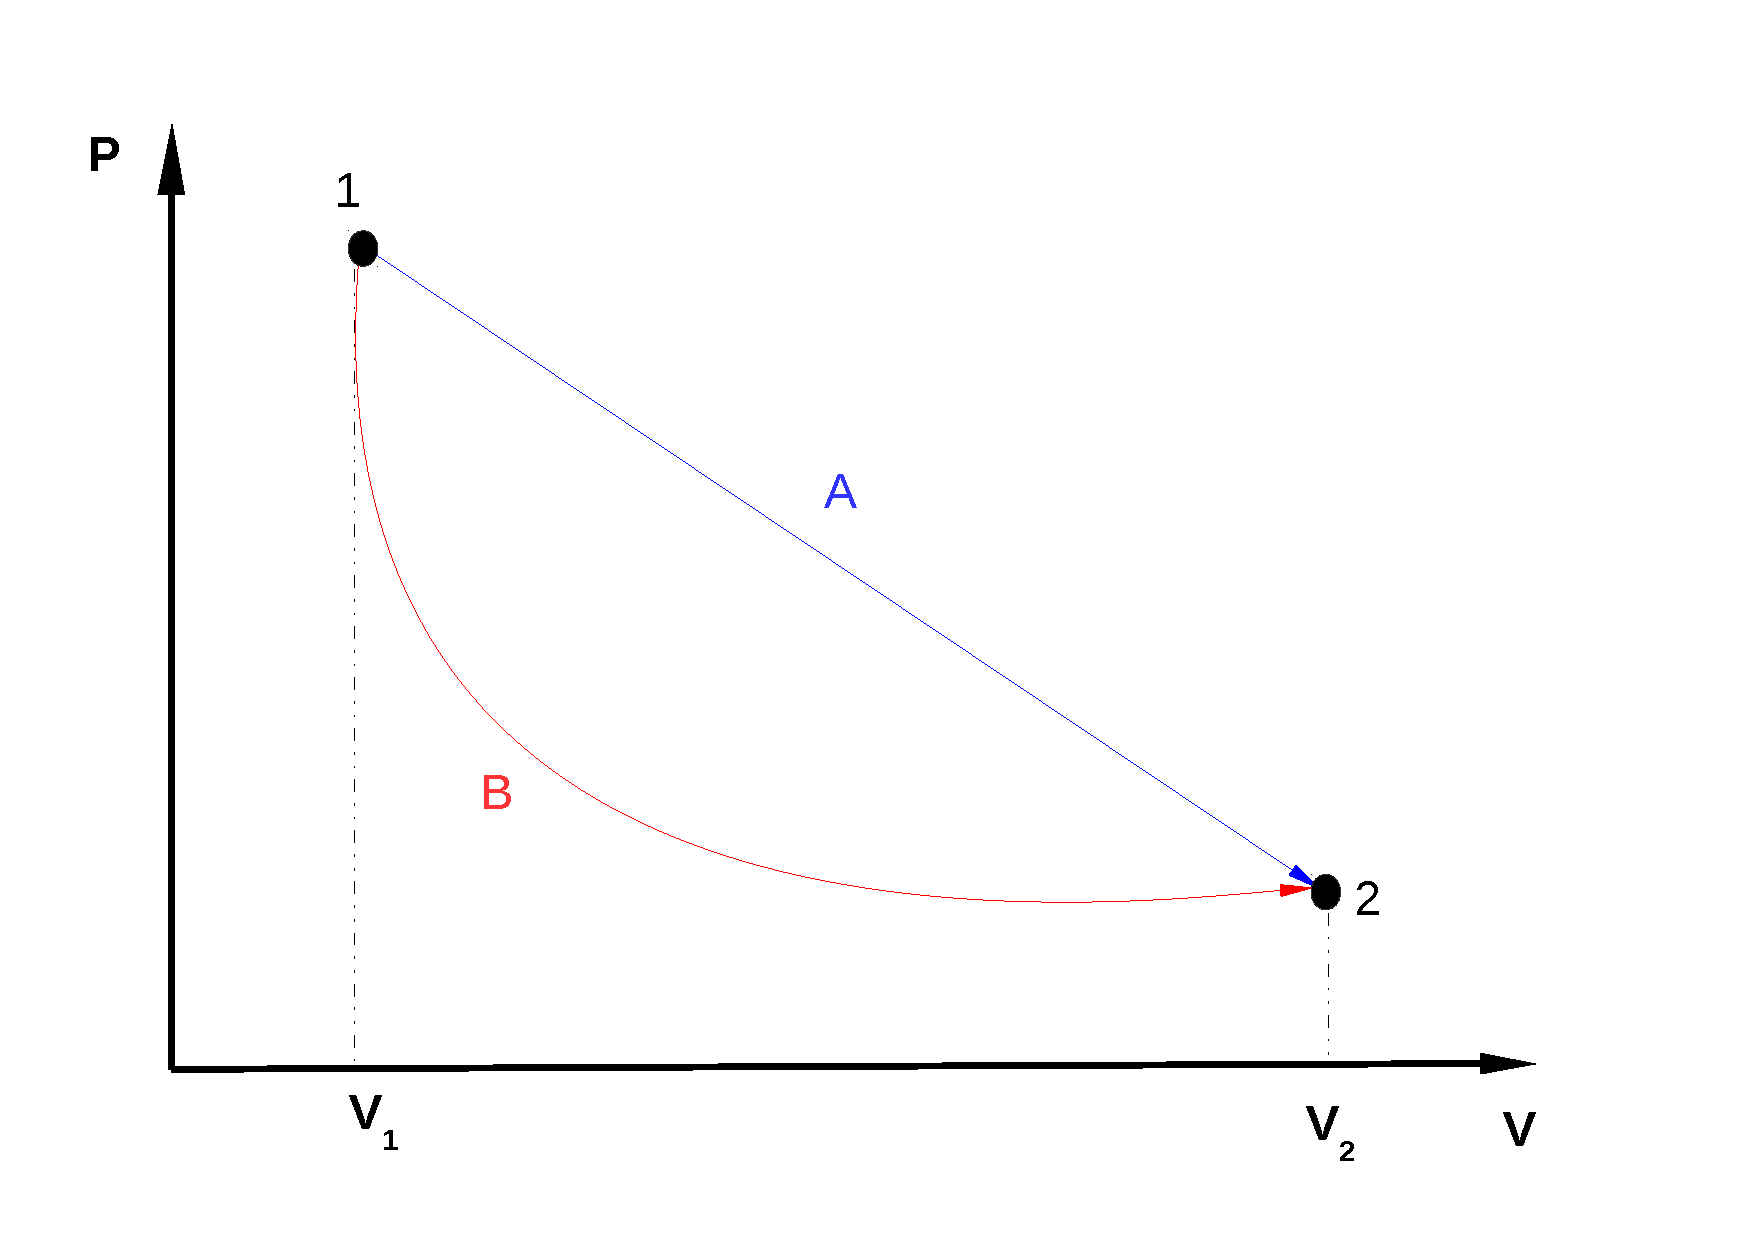
\includegraphics[width=0.7\columnwidth,clip]{./Figs/Chp3_PistonCylinder_PV}}}
        \caption{Gas expansion under different conditions represented by 2 paths.}\label{Chapter:FirstLaw:Fig:Work_PV}
   \end{figure}

   
%%%
%%% SECTION
%%%
   \section{Reversible Adiabatic Processes}\label{Chapter:FirstLaw:Section:ReversibleAdiabaticProcesses}\index{Process!Adiabatic}
     \begin{subequations}

       A process is named {\it adiabatic} when no heat is transferred to or from the system (\ie $\delta Q$ = 0),
         \begin{equation}
           dU = \cancelto{0}{\delta Q} + \delta W \;\;\Longrightarrow\;\; \Delta U = U_{2}-U_{1}= W.
         \end{equation}
       This equation is valid for both reversible and irreversible processes\index{Process!Reversible}\index{Process!Irreversible}, and can only be ensured if a perfect thermal insulation is achieved.  For mechanically reversible adiabatic (\ie isentropic) compression / expansion of ideal gases,
      \begin{eqnarray}
          dU &=& \delta Q + \delta W \;\;\Longrightarrow \;\; \delta Q = C_{v}dT + PdV = 0 \nonumber \\
          dT &=& -\frc{P}{C_{v}}dV  \;\; \left(\text{Constraint: } C_{v}\ne 0\right) \nonumber \\
             &=& -\frc{RT}{V C_{v}}dV \;\; \Rightarrow \;\; \frc{dT}{T} = - \frc{R}{C_{v}}\frc{dV}{V}. \label{Chapter:FirstLaw:Eqn:AdiabaticProcesses1}
      \end{eqnarray}
      Integrating Eqn.~\ref{Chapter:FirstLaw:Eqn:AdiabaticProcesses1} and assuming $C_{v}$ is constant,
           \begin{eqnarray}
              &&\int\limits_{T_{1}}^{T_{2}} \frc{dT}{T} = \frc{R}{C_{v}}\int\limits_{V_{1}}^{V_{2}}\frc{dV}{V} \;\;\Longrightarrow\;\;  \left.\ln{T}\right|_{T_{1}}^{T_{2}} = \left.-\frc{R}{C_{v}}\ln{V}\right|_{V_{1}}^{V_{2}}\nonumber \\
              &&\ln{\frc{T_{2}}{T_{1}}} = -\frc{R}{C_{v}}\ln{\frc{V_{2}}{V_{1}}} = \ln{\left(\frc{V_{1}}{V_{2}}\right)^{\frac{R}{C_{v}}}}\;\;\Longrightarrow\;\; \frc{T_{2}}{T_{1}} = \left(\frc{V_{1}}{V_{2}}\right)^{\frac{R}{C_{v}}} \nonumber
           \end{eqnarray}
           Now, using the ratio of specific heats defined in Eqn.~\ref{Chapter:FirstLaw:Eqn:HeatCapacitiesRelation_IdealGas2}, 
           \begin{displaymath}
              \gamma = 1 + \frc{R}{C_{v}},
           \end{displaymath}
           in the previous relation,
           \begin{shaded}
             \begin{equation}
                TV^{\gamma-1} = \text{ constant}\label{Chapter:FirstLaw:Eqn:AdiabaticProcesses_TVGamma}
             \end{equation}
           \end{shaded}

           Now from Eqn.~\ref{Chapter:FirstLaw:Eqn:HeatCapacitiesRelation_IdealGas3},
           \begin{displaymath}
               \delta Q = C_{p}dT - \frc{RT}{P}dP = 0,
           \end{displaymath}
           and assuming $C_{p}$ is constant and different from zero,
           \begin{eqnarray}
             && \int\limits_{T_{1}}^{T_{2}}\frc{dT}{T} = \frc{R}{C_{p}}\int\limits_{P_{1}}^{P_{2}}\frc{dP}{P} \;\;\Longrightarrow\;\; \left.\ln{T}\right|_{T_{1}}^{T_{2}} = \left.\frc{R}{C_{p}} \ln{P}\right|_{P_{1}}^{P_{2}} \nonumber \\
             && \ln{\frc{T_{2}}{T_{1}}} = \ln{\left(\frc{P_{2}}{P_{1}}\right)^{\frac{R}{C_{p}}}} \;\;\Longrightarrow\;\;  \frc{T_{2}}{T_{1}} = \left(\frc{P_{2}}{P_{1}}\right)^{\frac{R}{C_{p}}}.\nonumber
           \end{eqnarray}
           Again, using  Eqn.~\ref{Chapter:FirstLaw:Eqn:HeatCapacitiesRelation_IdealGas2},
           \begin{shaded}
             \begin{equation}
                TP^{\frac{1-\gamma}{\gamma}} = \text{ constant}\label{Chapter:FirstLaw:Eqn:AdiabaticProcesses_TPGamma}
             \end{equation}
           \end{shaded}
           
           Finally, integrating the right-hand side from Eqn.~\ref{Chapter:FirstLaw:Eqn:HeatCapacitiesRelation_IdealGas3},
           \begin{eqnarray}
               && \delta Q = \frc{C_{v}}{R}VdP + \frc{C_{p}}{R}PdV = 0 \;\; \Longrightarrow \;\; \frc{C_{v}}{\cancel{R}}VdP = -\frc{C_{p}}{\cancel{R}}PdV \;\;\Longrightarrow\;\; C_{v}\int\limits_{P_{1}}^{P_{2}} \frc{dP}{P} = -C_{p}\int\limits_{V_{1}}^{V_{2}}\frc{dV}{V} \nonumber \\
              && \left.\ln{P}\right|_{P_{1}}^{P_{2}} = -\left.\frc{C_{p}}{C_{v}}\ln{V}\right|_{V_{1}}^{V_{2}} \;\; \Longrightarrow \;\;\frc{P_{2}}{P_{1}} = \left(\frc{V_{1}}{V_{2}}\right)^{\frac{C_{p}}{C_{v}}}\nonumber 
           \end{eqnarray}
           Again, using  Eqn.~\ref{Chapter:FirstLaw:Eqn:HeatCapacitiesRelation_IdealGas2},
           \begin{shaded}
             \begin{equation}
                PV^{\gamma} = \text{ constant}\label{Chapter:FirstLaw:Eqn:AdiabaticProcesses_PVGamma}
             \end{equation}
           \end{shaded}
     \end{subequations}



   % Example
   \begin{MyExample}{\begin{center}{\bf Example}\end{center}}
     \begin{example}\label{Chapter:FirstLaw:Example8}\citep{Rajput_Book}
       Air initially occupying 1 m$^{3}$ at 1.5 bar and 20$^{\circ}$C undergoes an internally reversible compression for which $P V^{\gamma}=$ constant to a final state where the pressure is 6 bar and the temperature is 120$^{\circ}$C. Determine:
        \begin{enumerate}[(a)]
           \item Value of $\gamma$;
           \item Work and the heat transfer (in kJ).
       \end{enumerate}
       Assume that heat capacity at constant volume and molar mass of air are 0.718 kJ.$\left(\text{kg.K}\right)^{-1}$ and 29 g.mol$^{-1}$.
     \end{example}

% SOLUTION
       \noindent{\bf Solution:} 
        \begin{center}
           \begin{tabular}{c c c c}
               {\bf State}  &   $P$ (atm)  &   $T\;\left(^{\circ}\text{C}\right)$ & $V\;\left(\text{m}^{3}\right)$ \\
                    1       &     1.5      &            20                      & 1  \\
                    2       &     6.0      &            120                     &     \\              
           \end{tabular}
        \end{center}
        \begin{enumerate}[(a)]
           \item In order to calculate the isentropic index $\gamma$, we can use any of the relations learned in the lecture,
               \begin{displaymath} 
                   P V^{\gamma} = C, \hspace{1cm} T V^{\gamma-1} = C \hspace{1cm} \text{ and/or } \hspace{1cm} T P^{\frac{1-\gamma}{\gamma}} = C.
               \end{displaymath}
               Although $P$ and $V$ is the relation initially given in the problem, we do not know the final volume of air, $V_{2}$. However, initial and final pressure and temperature are known and we can make use of this relationship to obtain $\gamma$,
               \begin{eqnarray} 
                   T P^{\frac{1-\gamma}{\gamma}} = C \Rightarrow T_{1}P_{1}^{\frac{1-\gamma}{\gamma}} = T_{2}P_{2}^{\frac{1-\gamma}{\gamma}} \nonumber \\
                   \left(\frc{P_{1}}{P_{2}}\right)^{\frac{1-\gamma}{\gamma}} = \frc{T_{2}}{T_{1}} \Rightarrow \frc{1-\gamma}{\gamma} = \frc{\ln{\frac{T_{2}}{T_{1}}}}{\ln{\frac{P_{1}}{P_{2}}}} \Longrightarrow \gamma = 1.2686  \nonumber
               \end{eqnarray}
                 
           \item Compression work can be obtained by integrating $\d W = -P dV$ from state 1 to state 2 with $P=\frac{C}{V^{\gamma}}$,
               \begin{eqnarray}
                 W_{1-2} &=& -\int\limits_{V_{1}}^{V_{2}} P dV = -\int\limits_{V_{1}}^{V_{2}}\frc{C}{V^{\gamma}} dV = -\left.\frc{C}{1-\gamma}V^{1-\gamma}\right|_{V_{1}}^{V_{2}} \nonumber \\
                         &=& -\frc{C}{1-\gamma}\left(V_{2}^{1-\gamma}-V_{1}^{1-\gamma}\right),\;\;\text{ however, as } C=P_{1}V_{1}^{\gamma}=P_{2}V_{2}^{\gamma} \nonumber \\
                         &=& -\frc{P_{2}V_{2}^{\gamma}V_{2}^{1-\gamma} - P_{1}V_{1}^{\gamma}V_{1}^{1-\gamma}}{1-\gamma} = \frc{P_{1}V_{1}-P_{2}V_{2}}{1-\gamma} \nonumber
               \end{eqnarray}
               The relation above, although important, can not be used as we do not know $V_{2}$, however we can change variables through the ideal gas relation
               \begin{eqnarray}
                 P V = n R T &\Rightarrow& n = \frc{P V}{R T } = \frc{1.5\text{ atm} \times 1\text{ m}^{3}}{ 8.3143 \frc{\text{J}}{\text{mol.K}} 293.15\text{ K}} \frc{1.01325\times 10^{5} \text{ Pa}}{1 \text{ atm}} \frc{ 1 \text{ N.m}^{-2}}{1\text{ Pa}}\frc{1 \text{ J}}{1\text{ N.m}} \nonumber \\
                 &&  n = 62.3580\text{ moles} \nonumber \\
                   % m &=& \frc{P_{1} V_{1} MW}{R T_{1}} = \frc{1.5\text{ atm} \times 1\text{ m}^{3} \times 29 \frac{\text{g}}{\text{mol}} } { 8.3143 \frc{\text{J}}{\text{mol.K}} 293.15\text{ K}} \frc{1 \text{ J}}{1\text{ N.m}} \frc{1.01325\times 10^{5} \text{ Pa}}{1 \text{ atm}} \frc{ 1 \text{ N.m}^{-2}}{1\text{ Pa}} = 1808.38 \text{ g}\nonumber\\
                    W &=& \frc{P_{1}V_{1}-P_{2}V_{2}}{1-\gamma} = nR\frc{T_{1}- T_{2}}{1-\gamma} \nonumber \\
                      &=& 62.3580\text{ mol} \times 8.3143 \frc{\text{J}}{\text{mol.K}} \times \frc{\left(293.15-393.15\right)\text{ K}}{1-1.2686} \nonumber \\
                      &=& 193024.2440 \text{ J} \Longrightarrow W = -193.02 \text{ kJ} \nonumber
               \end{eqnarray}
              Heat ($Q$) can be obtained from
               \begin{eqnarray}
          \Delta u &=& m C_{v}\Delta T = n MW C_{v}\Delta T = Q + W  \nonumber \\
             Q &=& n MW C_{v}\left(T_{2}-T_{1}\right) - W \nonumber \\
               &=& 62.3580\text{ mol}\times 29 \frc{\text{g}}{\text{mol}} \red{\frc{1\text{ kg}}{1000\text{ g}}}\times 0.718\frc{\text{kJ}}{\text{kg.K}}\times (393.15-293.15)\text{ K} - 193.30 \text{ kJ} \nonumber \\
                                                          &=& -63.46\text{ kJ}. \nonumber                   
               \end{eqnarray}
        \end{enumerate}
   \end{MyExample}
   

   
\clearpage   
\begin{FinalSummaryBlock}{Summary}
    \begin{itemize}
       \item Work is the transfer of energy by motion against an opposing force;
       \item Heat is the transfer of energy as a result of temperature differences between the system and the surroundings;
       \item Internal energy is the energy stored in the components of the system. The internal energy of an ideal gas is a function of temperature only;
       \item The First Law of thermodynamics states that heat and work are mutually convertible, however as energy can not be either created or destroyed, the internal energy associated with an energy conversion remains constant, $dU = \delta q + \delta w$;
       \item The energy of an isolated system is always constant;
       \item A reversible change is a change that can be reversed by an infinitesimal modification of a variable. Maximum work is achieved in a reversible change;
       \item The enthalpy is defined as $H = U + PV$. The enthalpy change is the energy transferred as heat at constant pressure, $\Delta H = Q$;
       \item Heat capacity at constant volume is defined as $C_{v}=\left(\partial U / \partial T\right)_{V}$. The heat capacity at constant pressure is defined as $C_{p}=\left(\partial H / \partial T\right)_{P}$;
       \item In case of:
         \begin{itemize}
            \item Reversible isochoric process (\ie $V=$ constant):
              \begin{displaymath}
                \Delta U = C_{v}\left(T_{2}-T_{1}\right), \;\; W = 0\;\; Q = C_{v}\left(T_{2}-T_{1}\right);
              \end{displaymath}
            \item Reversible isobaric process (\ie $P=$ constant):
              \begin{displaymath}
                \Delta U = C_{v}\left(T_{2}-T_{1}\right), \;\; W = P\left(V_{2}-V_{1}\right)\;\; Q = C_{p}\left(T_{2}-T_{1}\right);
              \end{displaymath}
            \item Reversible adiabatic process (\ie $PV^{\gamma}=$ constant):
              \begin{displaymath}
                 \frc{T_{2}}{T_{1}} = \left(\frc{V_{1}}{V_{2}}\right)^{\gamma-1} = \left(\frc{P_{2}}{P_{1}}\right)^{\frc{\gamma-1}{\gamma}};
              \end{displaymath}
            \item Polytropic reversible process (\ie $PV^{n}=$ constant):
              \begin{displaymath}
                 \frc{T_{2}}{T_{1}} = \left(\frc{V_{1}}{V_{2}}\right)^{n-1} = \left(\frc{P_{2}}{P_{1}}\right)^{\frc{n-1}{n}}.
              \end{displaymath}
         \end{itemize}
    \end{itemize}
\end{FinalSummaryBlock}
 % Introduction to First Law of Thermodynamics
     \setcounter{examplecounter}{0}
  
%%%
%%% CHAPTER
%%%
\chapter{Second Law of Thermodynamics}\label{Chapter:FirstLaw}

   \begin{LearningObjectivesBlock}{Learning Objectives}
      Upon completion of this chapter, you will be able to
        \begin{enumerate}
           \item Demonstrate understanding of key concepts of energy and the first law of thermodynamics;
           \item Apply the first law of thermodynamics to assess of heat transfer and power cycles;
           \item Conduct energy analysis of thermodynamic systems;
           \item Employ energy and mass balances into thermodynamic systems to assess efficiency, and correctly observe sign conventions for work and heat transfer.
        \end{enumerate}
\medskip
     Recommended reading: Chapters 5 of \citet{SmithVanNess_Book,Moran_Book,Borgnakke_Book} or 3 of \citet{Atkins_Book}.
   \end{LearningObjectivesBlock}


  
%%%
%%% SECTION
%%%
   \section{Introduction}\label{Chapter:SecondLaw:Section:Intro}
   The first law (Chapters~\ref{Chapter:Introduction} and \ref{Chapter:FirstLaw}) demonstrated that energy can flow either from or to a system in the form of heat or work, however it does not indicate the direction of process (\ie energy flow). The second law of thermodynamics concerns about feasibility, direction and spontaneity of processes and entropy..
   
The second law of thermodynamics is a general principle which makes constraints upon spontaneity of the process, direction of heat transfer and general efficiency of heat engines, \eg a hot body cools to the temperature of the surroundings or a chemical reaction that may run in one direction instead of the reverse (\eg combustion of ethane producing carbon dioxide and water). The reverse of such processes may occur but they will not be spontaneous.  
  
%%%
%%% SECTION
%%%
   \section{Statement of the Second Law}\label{Chapter:SecondLaw:Section:SecondLawStatement}\index{Laws of Thermodynamics ! Second law}
The second law of thermodynamics was stated separately by \citet{Clausius_Book}, Kelvin \citep{Thomson_1851} and \citet{Planck_Book} in slightly different ways. Each statement is based on irreversible processes.
\begin{shaded}
  \begin{center}
    {\bf Clausius Statement}
  \end{center}
  'It is impossible for a self-acting machine working in a cyclic process unaided by any external agency, to convey heat from a body at a lower temperature to a body at a higher temperature.'
\end{shaded}
This statement clearly indicates that heat cannot spontaneously flow from a colder to a hotter body. This can only be realised if other effects play some role, \eg in a refrigeration process in which external work is used to extract heat from low temperature body and reject it into a high temperature body (Fig.~\ref{Chapter:SecondLaw:Fig:SecondLawStatement})

   %%% FIGURE
   \begin{figure}[h]
     \begin{center}
        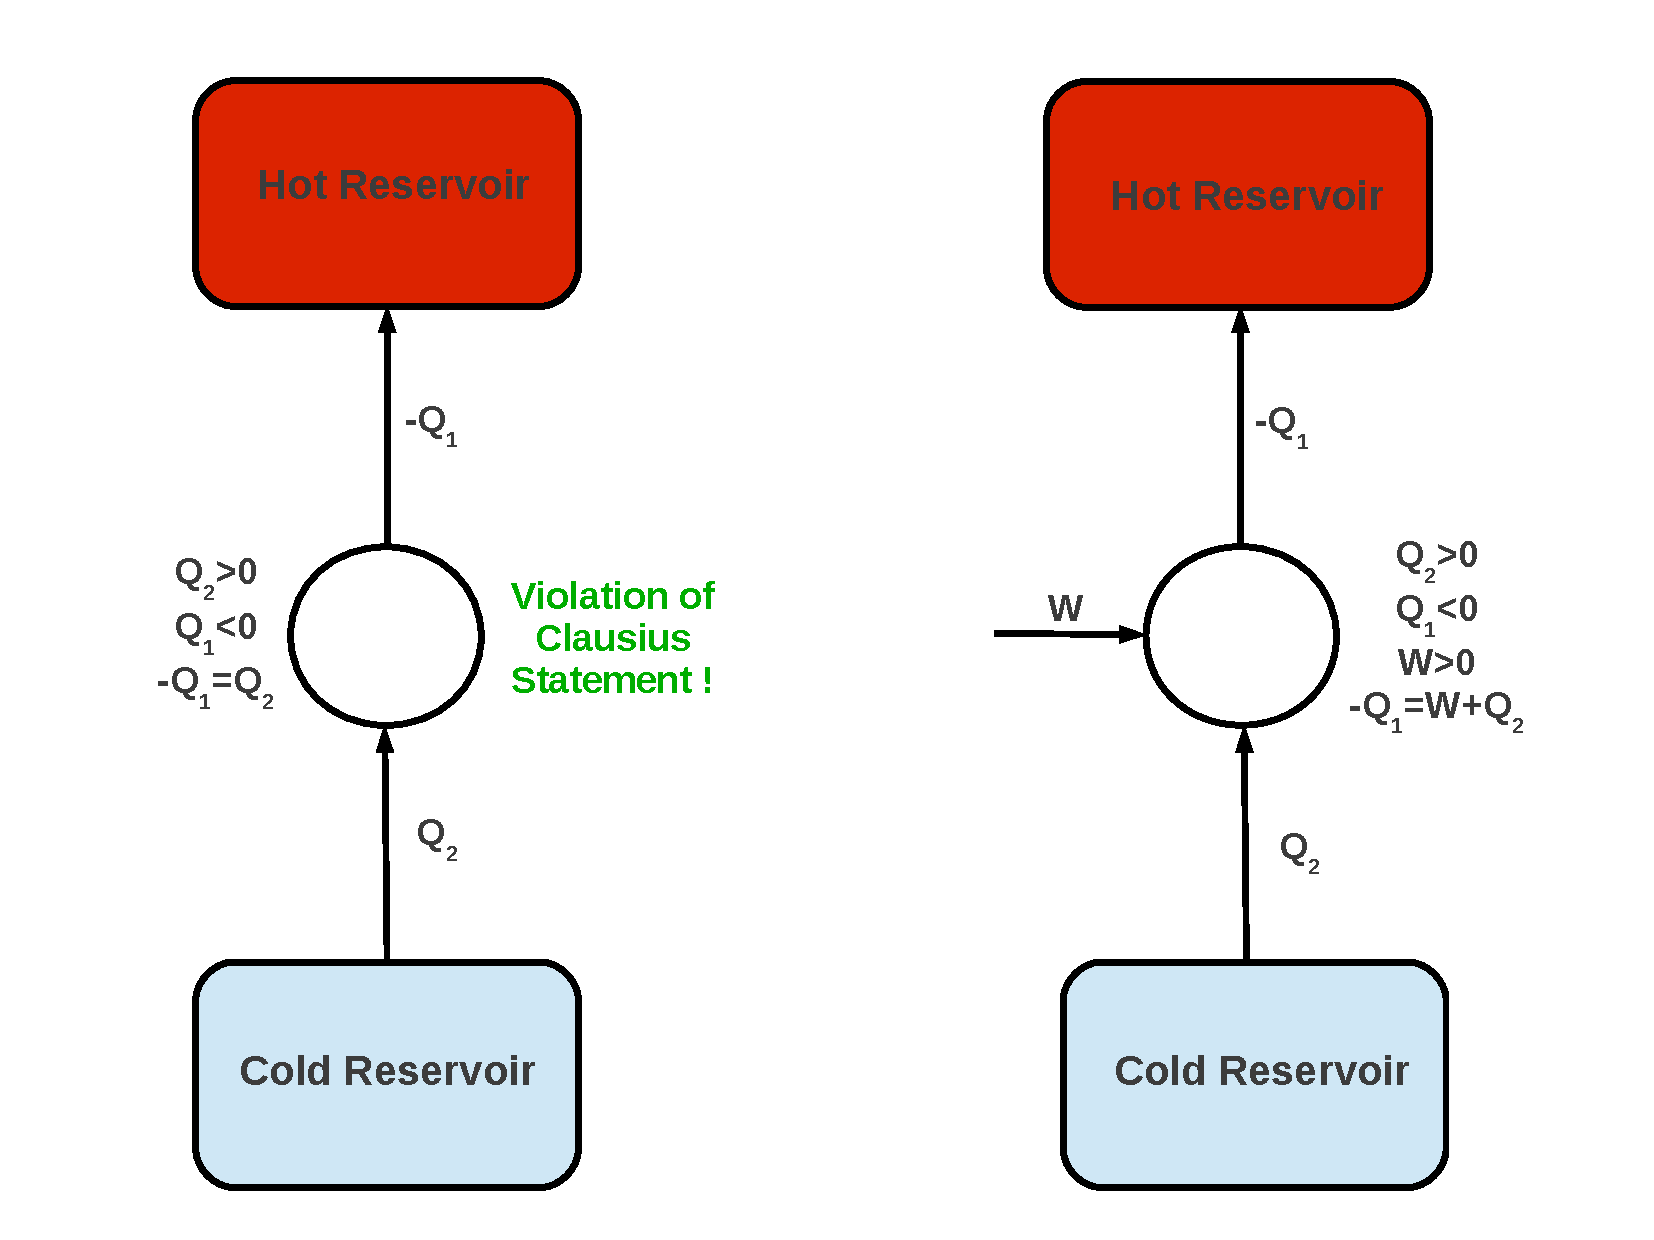
\includegraphics[width=.8\columnwidth,clip]{./Figs/2ndLaw_Schem}
     \caption{All spontaneous processes are irreversible -- heat flows from hot to cold spontaneously and irreversibly. }\label{Chapter:SecondLaw:Fig:SecondLawStatement}
     \end{center}
   \end{figure} 

\begin{shaded}
  \begin{center}
    {\bf Kelvin-Planck Statement}
  \end{center}
  'It is impossible to construct an engine, which while operating in a cycle produces no other effect except to extract heat from a single reservoir and do equivalent amount of work.'
\end{shaded}
This statement indicates that in order to achieve net work from a heat engine (\ie a device operating in cycle), there should be heat interaction between two bodies (\ie thermal reservoirs) at different temperatures (\ie thermal source or sink). 


%%%
%%% SECTION
%%%
   \section{Mathematical Statement of the Second Law}\label{Chapter:SecondLaw:Section:SecondLawStatement_Maths}\index{Laws of Thermodynamics ! Second law}
     \begin{subequations}
        In Fig.~\ref{Chapter:SecondLaw:Fig:SecondLawStatement2}, an infinitesimal amount of heat, $\delta Q^{\prime}$, is transferred from the thermal reservoir (with temperature $T_{res}$) to a reversible cyclic engine (1). The engine produces a small amount of work, $\delta W^{\prime}$, and releases an infinitesimal amount of heat, $\delta Q$ to another reservoir (at variable temperature $T$) that also releases energy in form of work $\left(\delta W\right)$ to the surroundings.


   %%% FIGURE
   \begin{figure}[h]
     \begin{center}
        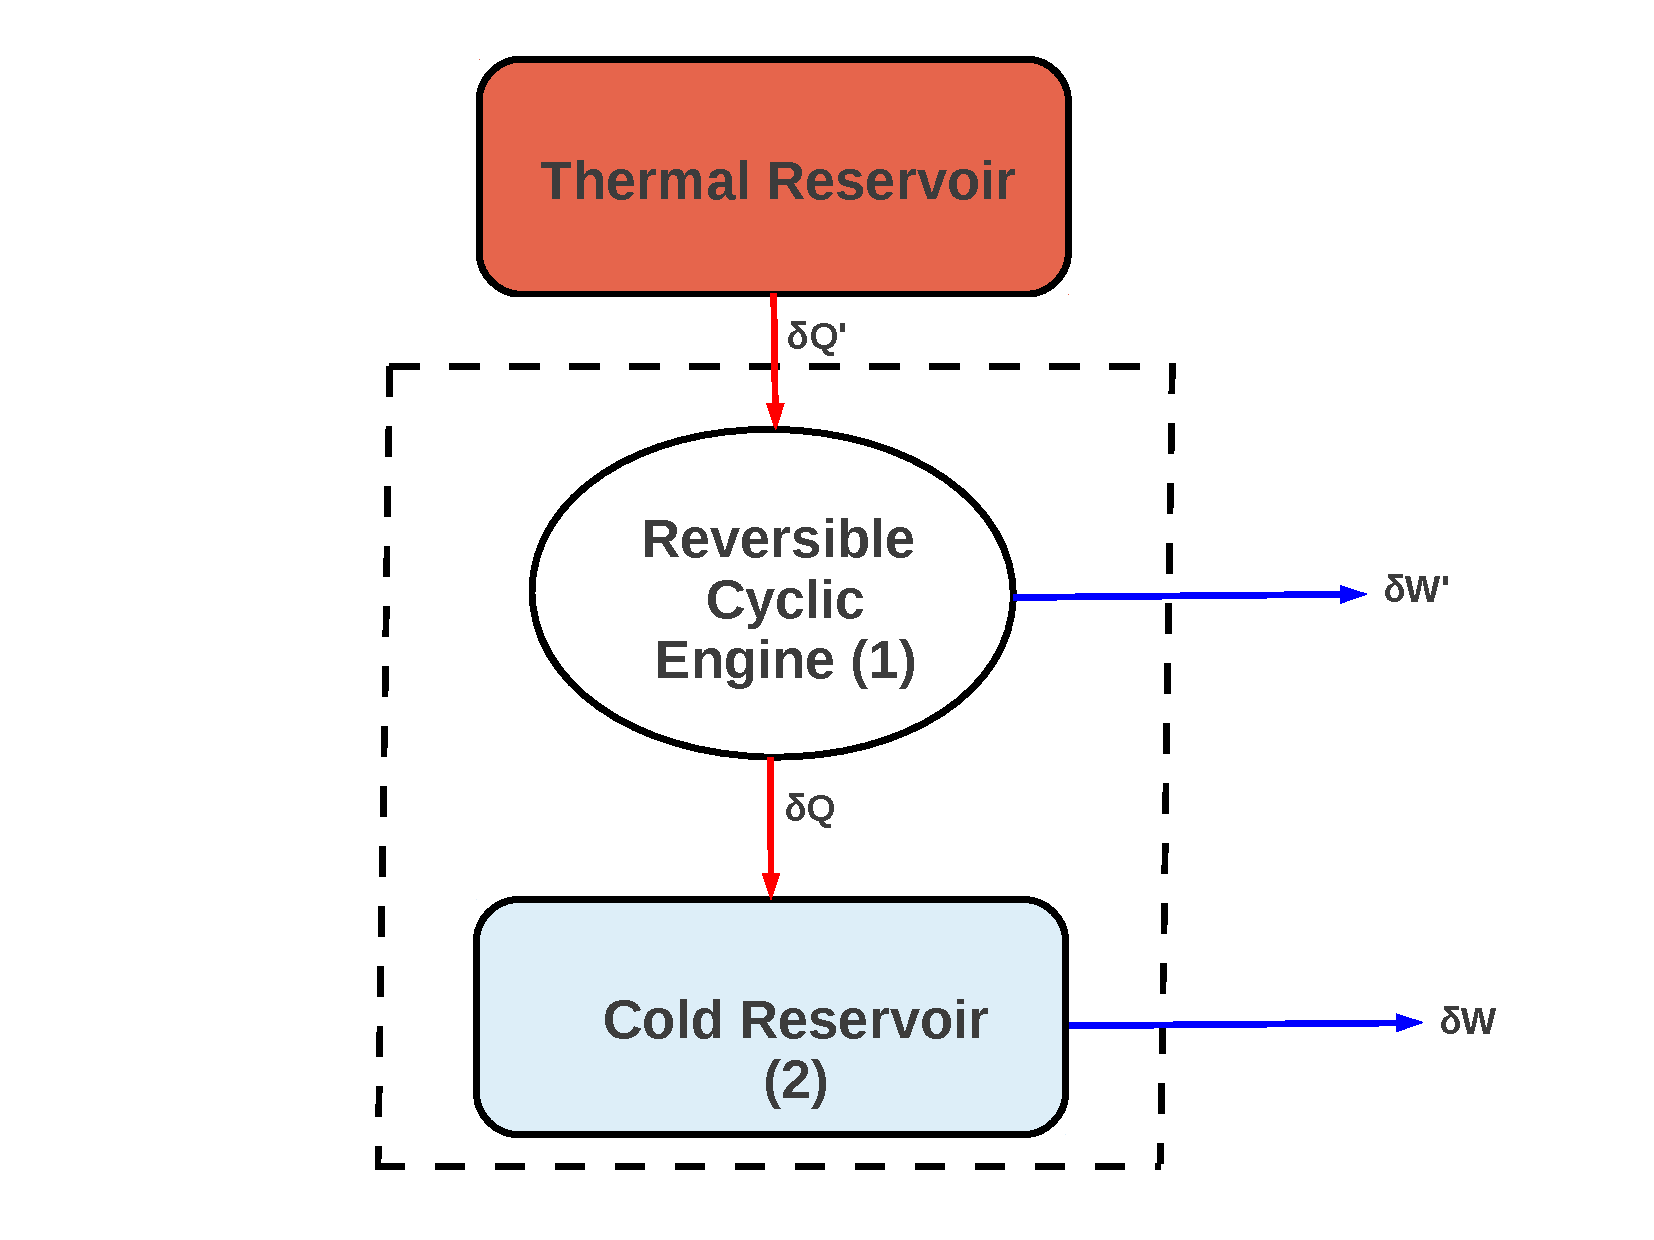
\includegraphics[width=.8\columnwidth,clip]{./Figs/2ndLaw_Schem2}
     \caption{Thermal device for mathematical derivation of the Second law. }\label{Chapter:SecondLaw:Fig:SecondLawStatement2}
     \end{center}
   \end{figure} 

     \end{subequations}
 % Introduction to Second Law of Thermodynamics
 
\makeatletter\@openrightfalse 
\extraPartText{\blue{(Contents of this Part are not examinable. They were designed to help with some of the notations and definitions used in the remaining of this Notes.)}} 
\part{Drivers of Geothermal Energy}  
     \setcounter{examplecounter}{0} 
     \setcounter{problemcounter}{0}
  
%%%
%%% CHAPTER
%%%
\chapter{Energy Sources and Drivers for Power Generation}\label{Chapter:EnergySourcesDrivers}

   \begin{LearningObjectivesBlock}{Learning Objectives}
      Upon completion of this chapter, you will be able to
        \begin{enumerate}
           \item Define 
        \end{enumerate}
\medskip
     Recommended reading: \citet{DiPippo_Book,Armstead_Book,Barbier_2002,Zarrouk_2014,Rybach_2003,Pollack_1993}
   \end{LearningObjectivesBlock}


%%%%%%%%%%%%%%%%%%%%%%%%%%%%%%%%%%%%%%%%%%%%%%%%%%%%%%%%%%%%%%%%%
\begin{comment}
   \begin{LearningObjectivesBlock}{Learning Objectives}
      Upon completion of this chapter, you will be able to
        \begin{enumerate}
           \item {\bf Knowledge:} Define, Name, Select, State 
           \item {\bf Comprehension:} Describe, Identify, Discuss
           \item {\bf Application:} Apply, Demonstrate, Employ, Sketch
           \item {\bf Analysis:} Analyse, Compare, Calculate, Solve
           \item {\bf Synthesis:} Determine, Formulate
           \item {\bf Evaluation:} Assess, Check, Estimate, Compare, Measure, Monitor
        \end{enumerate}
\end{comment}
%%%%%%%%%%%%%%%%%%%%%%%%%%%%%%%%%%%%%%%%%%%%%%%%%%%%%%%%%%%%%%%%%
  

%%%% ETOC
\localtableofcontents


%%%
%%% SECTION
%%%
\section{Introduction}\label{Chapter:EnergySourcesDrivers:Section:Intro}

Electricity is a critical commodity in the modern world -- illumination lighting, TVs, computers, electronic devices (and even cars) etc, they all rely on extensive sources of electricity. In the developed world, electricity is taken for granted, often at relatively low costs, whereas in developing countries cost, quality and availability of electricity are still a daily challenge. 

Coal and wood were burned in the earliest power plants to produce electricity. These rudimentary power plants were initially based on reciprocating steam engines\index{Reciprocating engines} with low overall efficiency, and later replaced by power plants operating with steam turbines. Hydro-power were introduced in the energy mix in the second-half of the nineteenth century as a natural development of its use as mechanical power in the new industrial age. Other energy technologies were further developed along the twentieth century with the introduction of refined hydrocarbons (diesel, natural gas etc) to (a) produce relatively cheap electricity; (b) transport of people and goods, and; (c) heat closed environments. Nuclear energy was first used to commercially generate electricity in 1957 (SM-1 Nuclear Power Plant at Virginia, USA), producing 2 MWe. Since then, nuclear technology has improved in power generation, efficiency and safety, and nowadays the world net capacity is of approximately 370 GWe. This represents nearly 6$\%$ of the world primary energy production, whereas other renewable energy resources such as biomass (\ie wood and dry crop wastes) and hydropower contribute about 10$\%$ and 7$\%$, respectively \citep{AER_2011}.\footnote{See also \href{https://www.imperial.ac.uk/people/r.bryan/document/2407/200barrelsleft2009/?200barrelsleft2009.pdf}{M. Blunt (2009) 'Two hundred barrels left: an analysis of population growth. oil reserves and carbon dioxide emissions'.}}
\medskip

Heat is a form of energy source that can be ``harvested'' from Earth core by geothermal power plants. 




blabla\footnote{See \href{https://www.imperial.ac.uk/people/r.bryan/document/2407/200barrelsleft2009/?200barrelsleft2009.pdf}{M. Blunt (2009) 'Two hundred barrels left: an analysis of population growth. oil reserves and carbon dioxide emissions'.}}


Geothermal energy is simply the natural heat that exists within our planet. In some parts of the
world the existence of a geothermal energy resource is made obvious by the presence of hot
springs, and such resources have been exploited in various ways for millennia. More usually,
there is no direct evidence at Earth‘s surface of the vast reservoir of stored heat below, and
geothermal energy has remained largely ignored and untapped in most parts of the world. Now,
its potential as a renewable source of energy is being recognised increasingly, and technologies
and concepts for exploiting it are developing rapidly along two lines: low temperature resources,
which exploit warm water in the shallow subsurface to provide heat either directly (as warm
water) or indirectly (via heat exchange systems); and high temperature resources, which yield
hot water, usually from deeper levels, that can be used to generate electricity.
The potential for harnessing electricity from geothermal energy has long been recognised; the
potentially substantial reserves, minimal environmental impact, and capacity to contribute
continuously to base load electricity supply make it an extremely attractive prospect. The
ongoing drive to develop renewable sources of energy, coupled with anticipated technological
developments that will in future reduce the depth at which heat reservoirs are considered
economically viable, means there is now a pressing need to know more about the deep
geothermal energy potential in Scotland.






The Energy and Climate Change Directorate (ECCD) of the Scottish Government (the Client)
have identified deep geothermal energy as a particularly important emerging renewable energy
technology that could have the potential to play a significant role in Scotland‘s future energy
provision.
Exploitation of deep geothermal heat energy could potentially deliver many benefits to Scotland,
including:
Reducing carbon emissions and helping Scotland build a sustainable low-carbon economy
in order to meet the legislative requirements for emissions reductions;
Increase the use of renewable heat to help exceed the targets set out in the 2020
Routemap for Renewable Energy in Scotland;
Potentially help to exceed the targets for renewable electricity production;
Become a viable alternative source of energy, improving local and national energy security
and reducing reliance on external sources of energy;
Help reduce fuel poverty through the use of district heating networks;
Regenerate brownfield sites, including in former mining and industrial areas;
Provide skilled employment opportunities, with cross-over with the oil and gas and
manufacturing sectors; and
Push Scotland towards the forefront in the technology required for exploiting deep
geothermal resources, particularly in areas previously considered as marginal or even not
viable.
To date, the extent and location of the potential deep geothermal resources has not been well
defined. In addition, potential commercial investment in development of deep geothermal energy
requires greater certainty on the current administrative framework, including clarification of legal
ownership of resources legal ownership, resource licensing, supportive planning and permitting
regimes, and financing.
 % Drivers and Energy Sources 
%     \setcounter{examplecounter}{0}
%     \setcounter{problemcounter}{0}
%  \chapter{Thermodynamic Properties of Pure Fluids}\label{Chapter:ThermodynamicPropertiesPureFluids}

   \begin{LearningObjectivesBlock}{Learning Objectives}
      Upon completion of this chapter, you will be able to
        \begin{enumerate}
           \item Define pure substances and thermodynamic phases;
           \item State the Gibbs phase rule and its use to define the number of degrees of freedom of a system;
           \item Identify phases and phase transitions in a diagram;
           \item Formulate the solution for thermodynamic problems involving the calculation of volume of pure substances;
           \item Select appropriate equation of state for a given problem/application;
        \end{enumerate}
\medskip
     Recommended reading: Chapters 3 of \citet{SmithVanNess_Book}, 6 of \citet{Sandler_Book}, 2 of \citet{Borgnakke_Book} or 4 of \citet{Atkins_Book}.
   \end{LearningObjectivesBlock}


%%%%%%%%%%%%%%%%%%%%%%%%%%%%%%%%%%%%%%%%%%%%%%%%%%%%%%%%%%%%%%%%%
\begin{comment}
   \begin{LearningObjectivesBlock}{Learning Objectives}
      Upon completion of this chapter, you will be able to
        \begin{enumerate}
           \item {\bf Knowledge:} Define, Name, Select, State 
           \item {\bf Comprehension:} Describe, Identify, Discuss
           \item {\bf Application:} Apply, Demonstrate, Employ, Sketch
           \item {\bf Analysis:} Analyse, Compare, Calculate, Solve
           \item {\bf Synthesis:} Determine, Formulate
           \item {\bf Evaluation:} Assess, Check, Estimate, Compare, Measure, Monitor
        \end{enumerate}
\end{comment}
%%%%%%%%%%%%%%%%%%%%%%%%%%%%%%%%%%%%%%%%%%%%%%%%%%%%%%%%%%%%%%%%%

%%%% ETOC
\localtableofcontents
   

%%% SECTION
\section{Introduction}\label{Chapter:ThermodynamicPropertiesPureFluids:Section:Introduction}
   This chapter is an introduction to some of the mathematical underpinnings of chemical thermodynamics. Practical applications of most of the contents of this chapters may not be promptly obvious, however this is critical to fully understand concepts, theories and practices that will be introduced in later chapters. MORE!!

%%% SECTION
\section{Thermodynamic Property Relations for Single Phase Systems}\label{Chapter:ThermodynamicPropertiesPureFluids:Section:ThermodynamicPropertiesSinglePhase}
     \begin{subequations}

In Chapter~\ref{Chapter:FirstLaw}, we have learnt that the First Law for reversible processes in closed systems can be written as (for $n$ moles),
   \begin{equation}
       d\left(n U\right) = d Q_{\text{rev}} + d W_{\text{rev}},\label{Chapter:ThermodynamicPropertiesPureFluids:Eqn:FirstLaw}
   \end{equation} 
with $d W_{\text{rev}} = -Pd(nV)$ and $d Q_{\text{rev}}=Td(nS)$,
   \begin{equation}
       d\left(n U\right) = T d(nS) - Pd(nV).\label{Chapter:ThermodynamicPropertiesPureFluids:Eqn:FirstSecondLaw}
   \end{equation} 
This relation involves {\it only state functions}, therefore it is not restricted to reversible processes. The only constraint of this relation is that it is defined for closed systems and it assumes that changes may occur between equilibrium states. Finally, Eqn.~\ref{Chapter:ThermodynamicPropertiesPureFluids:Eqn:FirstSecondLaw} involves five thermodynamic properties: $P, T, V, U$ and $S$, and for $n=1$ mol, it becomes,
   \begin{shaded}
     \begin{equation}
        TdS = dU + PdV,\label{Chapter:ThermodynamicPropertiesPureFluids:Eqn:FundamentalRelation01}
     \end{equation}
   \end{shaded}
however, we know the definition of enthalpy,
     \begin{displaymath}
        dH = dU + d(PV) = dU + PdV + VdP.
     \end{displaymath}
Replacing this relation in Eqn.~\ref{Chapter:ThermodynamicPropertiesPureFluids:Eqn:FundamentalRelation01},
   \begin{shaded}
     \begin{equation}
        TdS = dH - VdP.\label{Chapter:ThermodynamicPropertiesPureFluids:Eqn:FundamentalRelation02}
     \end{equation}
   \end{shaded}
Equations~\ref{Chapter:ThermodynamicPropertiesPureFluids:Eqn:FundamentalRelation01}-\ref{Chapter:ThermodynamicPropertiesPureFluids:Eqn:FundamentalRelation02} correlate entropy changes to changes in other thermodynamic properties
      \begin{eqnarray}
         && dU = TdS - PdV \nonumber \\
         && dH = TdS + VdP. \nonumber 
      \end{eqnarray}
These two fundamental relations can be used to define the two remaining thermodynamic potentials, Gibbs ($G$) free and Helmholtz free ($A$) energy functions as:\index{Gibbs free energy! Definition}\index{Helmholtz free energy}
      \begin{eqnarray}
         && A \equiv U -TS \nonumber \\
         && G \equiv H -TS, \nonumber 
      \end{eqnarray}
or in differential form,
      \begin{eqnarray}
        && dA = dU -TdS - SdT \nonumber \\
        && dG = dH -TdS - SdT.\nonumber 
      \end{eqnarray}
Using Eqns.~\ref{Chapter:ThermodynamicPropertiesPureFluids:Eqn:FundamentalRelation01}-\ref{Chapter:ThermodynamicPropertiesPureFluids:Eqn:FundamentalRelation02}:
   \begin{shaded}
      \begin{eqnarray}
        && dA = - SdT - PdV, \label{Chapter:ThermodynamicPropertiesPureFluids:Eqn:HelmholtzFundamentalRelation01}\\ 
        && dG = - SdT + VdP. \label{Chapter:ThermodynamicPropertiesPureFluids:Eqn:GibbsFundamentalRelation01}
      \end{eqnarray}
   \end{shaded}
These four equations, Eqns.~\ref{Chapter:ThermodynamicPropertiesPureFluids:Eqn:FundamentalRelation01}-~\ref{Chapter:ThermodynamicPropertiesPureFluids:Eqn:GibbsFundamentalRelation01} are known as {\it fundamental thermodynamic relations} as they correlate the five thermodynamic potentials -- $U$, $H$, $S$, $G$, and $A$ with $PVT$ properties.\index{Fundamental thermodynamic relations}


     \end{subequations}

%%% SECTION
     \section{Maxwell Relations}\label{Chapter:ThermodynamicPropertiesPureFluids:Section:MaxwellRelations}
     \begin{subequations}

The thermodynamic potentials expressed in the four fundamental relations (Eqns.~\ref{Chapter:ThermodynamicPropertiesPureFluids:Eqn:FundamentalRelation01}-~\ref{Chapter:ThermodynamicPropertiesPureFluids:Eqn:GibbsFundamentalRelation01}) can be defined as a general functional, 
   \begin{displaymath}
    f = f(a,b),
   \end{displaymath}
with the assumption that the thermodynamic potentials, $f$, are continuous (and differentiable) throughout the domain. Therefore, we can write the total derivative\footnote{Total derivative along with the main elements of Calculus is briefly defined in Appendix~\ref{Appendix_Calculus:TotalDifferential}.} of function $f$ as
   \begin{equation}
         df = \underbrace{\left(\frc{\partial f}{\partial a}\right)_{b}}_{M}da + \underbrace{\left(\frc{\partial f}{\partial b}\right)_{a}}_{N}db = Mda + Ndb.\label{Chapter:ThermodynamicPropertiesPureFluids:Eqn:EqualRelation0}
   \end{equation}
Now, if we differentiate $M$ \wrt $b$ and $N$ \wrt $a$,
   \begin{displaymath}
         \left(\frc{\partial M}{\partial b}\right)_{a} = \frc{\partial^{2}f}{\partial a\partial b} \;\;\;\text{ and }\;\;\; \left(\frc{\partial N}{\partial a}\right)_{b} = \frc{\partial^{2}f}{\partial b\partial a},
   \end{displaymath}
since we required that $f(a,b)$ to be \underline{continuous}, 
   \begin{equation}
         \frc{\partial^{2}f}{\partial a\partial b} = \frc{\partial^{2}f}{\partial b\partial a}\;\;\Longrightarrow \left(\frc{\partial M}{\partial b}\right)_{a} = \left(\frc{\partial N}{\partial a}\right)_{b}\label{Chapter:ThermodynamicPropertiesPureFluids:Eqn:EqualRelation}
   \end{equation}
Now applying Eqn.~\ref{Chapter:ThermodynamicPropertiesPureFluids:Eqn:EqualRelation} into ~\ref{Chapter:ThermodynamicPropertiesPureFluids:Eqn:FundamentalRelation01},
   \begin{displaymath}
       \begin{cases}
          df = Mda + Ndb, & \\
          dU = TdS - PdV, &
       \end{cases}
   \end{displaymath}
with $M=T$, $da=dS$, $N=-P$, $db = dV$ and $df = dU$ leading to,
      \begin{shaded}
         \begin{equation}
            \left(\frc{\partial M}{\partial b}\right)_{a} = \left(\frc{\partial N}{\partial a}\right)_{b} \;\;\;\Longrightarrow \left(\frc{\partial T}{\partial V}\right)_{S} = - \left(\frc{\partial P}{\partial S}\right)_{V}\label{Chapter:ThermodynamicPropertiesPureFluids:Eqn:MaxwellRelation1}
         \end{equation}
Using the same procedure with  Eqn.~\ref{Chapter:ThermodynamicPropertiesPureFluids:Eqn:FundamentalRelation02}-~\ref{Chapter:ThermodynamicPropertiesPureFluids:Eqn:GibbsFundamentalRelation01},
           \begin{eqnarray}
              \left(\frc{\partial T}{\partial P}\right)_{S} &=& \left(\frc{\partial V}{\partial S}\right)_{P},\label{Chapter:ThermodynamicPropertiesPureFluids:Eqn:MaxwellRelation2} \\
              \left(\frc{\partial S}{\partial V}\right)_{T} &=& \left(\frc{\partial P}{\partial T}\right)_{V},\label{Chapter:ThermodynamicPropertiesPureFluids:Eqn:MaxwellRelation3} \\
              -\left(\frc{\partial S}{\partial P}\right)_{T} &=& \left(\frc{\partial V}{\partial T}\right)_{P},\label{Chapter:ThermodynamicPropertiesPureFluids:Eqn:MaxwellRelation4} 
           \end{eqnarray}
      \end{shaded}
Equations~\ref{Chapter:ThermodynamicPropertiesPureFluids:Eqn:MaxwellRelation1}-~\ref{Chapter:ThermodynamicPropertiesPureFluids:Eqn:MaxwellRelation4} are called as \blue{Maxwell relations}, and they allow determining changes in entropy without directly measurement, but only with changes on the PVT properties. We can also make use of the total derivative definition and apply it into Eqns.~\ref{Chapter:ThermodynamicPropertiesPureFluids:Eqn:FundamentalRelation01}-~\ref{Chapter:ThermodynamicPropertiesPureFluids:Eqn:GibbsFundamentalRelation01}, thus
   \begin{eqnarray}
                      &                            df =  \left(\frc{\partial f}{\partial a}\right)_{b}da + \left(\frc{\partial f}{\partial b}\right)_{a}db& \nonumber \\
      dU = TdS - PdV  &\;\;\;\Longleftrightarrow \;\;\;& dU =  \underbrace{\left(\frc{\partial U}{\partial S}\right)_{V}}_{T}dS + \underbrace{\left(\frc{\partial U}{\partial V}\right)_{S}}_{-P}dV \nonumber \\
      dH = TdS + VdP  &\;\;\;\Longleftrightarrow \;\;\;& dH =  \underbrace{\left(\frc{\partial H}{\partial S}\right)_{P}}_{T}dS + \underbrace{\left(\frc{\partial H}{\partial P}\right)_{S}}_{V}dP \nonumber \\
      dA = -SdT - PdV &\;\;\;\Longleftrightarrow \;\;\;& dA =  \underbrace{\left(\frc{\partial A}{\partial T}\right)_{V}}_{-S}dT + \underbrace{\left(\frc{\partial A}{\partial V}\right)_{T}}_{-P}dV \nonumber \\
      dG = -SdT + VdP &\;\;\;\Longleftrightarrow \;\;\;& dG =  \underbrace{\left(\frc{\partial G}{\partial T}\right)_{P}}_{-S}dT + \underbrace{\left(\frc{\partial G}{\partial P}\right)_{T}}_{V}dP \nonumber 
   \end{eqnarray}
Therefore
   \begin{shaded}
         \begin{eqnarray}
             \left(\frc{\partial U}{\partial S}\right)_{V} & =  T = & \left(\frc{\partial H}{\partial S}\right)_{P}\label{Chapter:ThermodynamicPropertiesPureFluids:Eqn:MaxwellRelation5} \\
             \left(\frc{\partial U}{\partial V}\right)_{S} & = -P = & \left(\frc{\partial A}{\partial V}\right)_{T}\label{Chapter:ThermodynamicPropertiesPureFluids:Eqn:MaxwellRelation6} \\
             \left(\frc{\partial H}{\partial P}\right)_{S} & =  V = & \left(\frc{\partial G}{\partial P}\right)_{T}\label{Chapter:ThermodynamicPropertiesPureFluids:Eqn:MaxwellRelation7} \\
             \left(\frc{\partial A}{\partial T}\right)_{V} & = -S = & \left(\frc{\partial G}{\partial T}\right)_{P}\label{Chapter:ThermodynamicPropertiesPureFluids:Eqn:MaxwellRelation8}
         \end{eqnarray}
   \end{shaded}
These property relations, Eqns.~\ref{Chapter:ThermodynamicPropertiesPureFluids:Eqn:MaxwellRelation5}-~\ref{Chapter:ThermodynamicPropertiesPureFluids:Eqn:MaxwellRelation8}, easily correlate measurable properties ($P$, $V$ and $T$) with non-measurable potentials ($U$, $H$, $S$, $A$ and $G$).

      \end{subequations}


   % Example
   \begin{MyExample}{\begin{center}{\bf Example}\end{center}}
     \begin{example}\label{Chapter:ThermodynamicPropertiesPureFluids:Example1} \citep{Balmer_Book}
         Suppose we make a series of measurements in the laboratory and think we discovered a new thermodynamic property, call it $\eta$. Our experimental data provide an empirical equation of the form,
          \begin{displaymath}
             d\eta = PdV + V^{2}dP
          \end{displaymath}
          Is $\eta$ a new property?
     \end{example}

% SOLUTION
       \noindent{\bf Solution:}
        The unknown is whether or not $\eta$ is a new thermodynamic property. Using Eqn.~\ref{Chapter:ThermodynamicPropertiesPureFluids:Eqn:EqualRelation0},
        \begin{displaymath}
            d\eta = Mda + Ndb = PdV + V^{2}dP,
        \end{displaymath}
        with $M=P$, $N=V^{2}$, $a=V$ and $b=P$. The cross differentials are
        \begin{displaymath}
            \Partial[M]{b}{a} = \Partial[P]{P}{V} = 1\;\;\;\text{ and }\;\;\; \Partial[N]{a}{b} = \Partial[V^{2}]{V}{P} = 2V \ne \Partial[M]{b}{a}.
        \end{displaymath}
         Since this equality is not satisfied, $\eta$ can not be a thermodynamic property.
   \end{MyExample}
   
   % Example
   \begin{MyExample}{\begin{center}{\bf Example}\end{center}}
     \begin{example}\label{Chapter:ThermodynamicPropertiesPureFluids:Example2} 
         A block of copper of 1 kg undertakes a reversible compression from 0.1 MPa to 100 MPa at constant temperature of 15$^{\circ}$C. Calculate:
    \begin{enumerate}[a)]
       \item Work done on the copper block during the process;
       \item Change in entropy {\it per} kg of copper;
       \item Heat transfer and;
       \item Change of internal energy {\it per} kg.
    \end{enumerate}
    Given, 
    \begin{itemize}
       \item Volume expansivity coefficient: $\beta = 5\times 10^{-5}$ K$^{-1}$;
       \item Isothermal compressibility coefficient: $\kappa = 8.6\times 10^{-12}$ m$^{2}$.N$^{-1}$;
       \item specific volume: $v=1.14\times 10^{-4}$ m$^{3}$.kg$^{-1}$.
    \end{itemize} 
     \end{example}

% SOLUTION
       \noindent{\bf Solution:}
       \begin{enumerate}[a)]
%
            \item The work done during the compression,
                \begin{displaymath}
                   w = -\int P dv,
                \end{displaymath}
                where $v$ is the specific volume. $\kappa$ was defined in Eqn.~\ref{Chapter:VolumetricPropertiesPureSubstances:Eqn:CompressibilityExpansivity} as,
                \begin{displaymath}
                   \kappa = \frc{1}{v}\left(\frc{\partial v}{\partial P}\right)_{T}\;\Longrightarrow \; v\kappa dP = - dv \;\;\text{ (with constant T)}
                \end{displaymath}
                For isothermal processes
                \begin{displaymath}
                   w = -\int P dv = - \int P\left(-v\kappa dP\right) = \frc{v}{2}\kappa\left(P_{2}^{2}-P_{1}^{2}\right) = 4.90\text{ J.kg}^{-1}
                \end{displaymath}
%
            \item $ds$ = ? (specific entropy).\\
                  From the Maxwell relations -- Eqn.~\ref{Chapter:ThermodynamicPropertiesPureFluids:Eqn:MaxwellRelation4}, 
                \begin{displaymath}
                   -\left(\frc{\partial s}{\partial P}\right)_{T} = \left(\frc{\partial v}{\partial T}\right)_{P},
                \end{displaymath}
                and from the definition of $\beta$,
                \begin{eqnarray}
                    && \beta = \frc{1}{v}\left(\frc{\partial v}{\partial T}\right)_{P} \;\;\Longrightarrow\;\; -\left(\frc{\partial s}{\partial P}\right)_{T} = \beta v \nonumber \\
                    && ds = -\beta v dP \;\;\Longrightarrow ds = s_{2}-s_{1} = -\beta v \left(P_{2}-P_{1}\right) = -0.5694 \text{ J.(kg.K)}^{-1} \nonumber
                \end{eqnarray}
%
            \item The heat transferred in such reversible isothermal process is
                \begin{displaymath}
                   dq = Tds \;\;\Longrightarrow q = T\left(s_{2}-s_{1}\right) = -164.07 \text{ J.kg}^{-1}.
                \end{displaymath}
%
            \item The specific internal energy,
                \begin{eqnarray}
                   &&  du = q + w \nonumber \\
                   && \left(u_{2}-u_{1}\right) = \underbrace{-164.07}_{\text{heat removed from the system}} + \overbrace{4.90}^{\text{work given to the system}} = -159.17 \text{ J.kg}^{-1}. \nonumber
                \end{eqnarray}
       \end{enumerate}
   \end{MyExample}
   

   % Example
   \begin{MyExample}{\begin{center}{\bf Example}\end{center}}
     \begin{example}\label{Chapter:ThermodynamicPropertiesPureFluids:Example3}  
     Demonstrate that the derivative of molar volume \wrt temperature at constant pressure is
     \begin{displaymath}
         \Partial[V]{T}{P} = -\frc{\Partial[P]{T}{V}}{\Partial[P]{V}{T}},
     \end{displaymath}
     and obtain an expression, $\Partial[V]{T}{P}$, for the van der Waals EOS. 

     \noindent{\bf Hint:} You should start the proof from the total differential of a continuous function $f(a,b)$,
     \begin{displaymath}
         df = \Partial[f]{a}{b}da + \Partial[f]{b}{a}db.
     \end{displaymath}
     \end{example}

% SOLUTION
       \noindent{\bf Solution:}
     The total differential of a generic continuous function $f(a,b)$ is
     \begin{displaymath}
         df = \Partial[f]{a}{b}da + \Partial[f]{b}{a}db.
     \end{displaymath}
     where (from the given thermodynamic function) $f=P$, $a=T$ and $b=V$, \ie
     \begin{displaymath}
         dP = \Partial[P]{T}{V}dT + \Partial[P]{V}{T}dV.
     \end{displaymath}
     However we want a differential expression in which $P$ is constant, therefore $dP = 0$,
     \begin{eqnarray}
         0 &=& \Partial[P]{T}{V}dT + \Partial[P]{V}{T}dV \;\;\;\text{ at } P \text{ constant},\nonumber \\
         \Partial[V]{T}{P} &=& -\frc{\Partial[P]{T}{V}}{\Partial[P]{V}{T}}.\nonumber
     \end{eqnarray}

     \medskip\noindent
     The vdW-EOS is,
     \begin{displaymath}
          P = \frc{RT}{V-b} - \frc{a}{V^{2}},
     \end{displaymath}
     where $V$ is the molar volume and $a$ and $b$ are constants that {\it depends only on critical properties}, $P_{c}$ and $T_{c}$. Due to the non-linearity of this EOS, obtaining $\Partial[V]{T}{P}$ from a direct differentiation would be difficult. However, we can use the expression that we just derived,
     \begin{displaymath}
         \Partial[V]{T}{P} = -\frc{\Partial[P]{T}{V}}{\Partial[P]{V}{T}} = -\frc{\frc{R}{V-b}}{-\frc{RT}{\left(V-b\right)^{2}}+\frc{2a}{V^{3}}}
     \end{displaymath} 

   \end{MyExample}


%%% SECTION
   \section{Relations for Internal Energy, Enthalpy and Entropy}\label{Chapter:ThermodynamicPropertiesPureFluids:Section:U_H_S_Relations}

%%% Subsection
     \subsection{Enthalpy and Entropy}\label{Chapter:ThermodynamicPropertiesPureFluids:Section:H_S_Relations}
      \begin{subequations}

Maxwell relations can help to develop relations for changes in $U$, $H$ and $S$ that reflect in heat and work interactions. Given
    \begin{displaymath}
       \begin{cases}
           H = H(T,P), &  \\
           S = S(T,P), &
        \end{cases} 
    \end{displaymath}
    \ie defining {\it enthalpy} and {\it entropy} as functions of temperature and pressure. Using Eqn.~\ref{Chapter:ThermodynamicPropertiesPureFluids:Eqn:FundamentalRelation02},
    \begin{displaymath}
      dH = TdS + VdP,
    \end{displaymath}
    at constant pressure and multiplying by $(1/dT)$,
    \begin{eqnarray}
        \Partial[H]{T}{P} &=& C_{p} = T\Partial[S]{T}{P} \nonumber \\
        \Partial[S]{T}{P} &=& \frc{C_{p}}{T}.\label{Chapter:ThermodynamicPropertiesPureFluids:Eqn:DerivedEntropyRelation1}
    \end{eqnarray}
Nowm using Eqn.~\ref{Chapter:ThermodynamicPropertiesPureFluids:Eqn:FundamentalRelation02} at constant $T$, multiplied by $(1/dP)$,
    \begin{displaymath}
       \Partial[H]{P}{T} = T\underbrace{\Partial[S]{P}{T}}_{\text{Eqn.~\ref{Chapter:ThermodynamicPropertiesPureFluids:Eqn:MaxwellRelation4}}} + V = -T\Partial[V]{T}{P} + V.
    \end{displaymath}
    
      \begin{shaded}
Now if we write the total derivative of function $H$,
    \begin{displaymath}
       dH = \Partial[H]{T}{P}dT + \Partial[H]{P}{T}dP 
    \end{displaymath}
         \begin{equation}
            dH = C_{p}dT + \left[V - T\Partial[V]{T}{P}\right]dP.\label{Chapter:ThermodynamicPropertiesPureFluids:Eqn:DerivedEnthalpyRelation1}
         \end{equation}
      \noindent
And the total derivative of function $S$ can be expressed as (using Eqn.~\ref{Chapter:ThermodynamicPropertiesPureFluids:Eqn:DerivedEntropyRelation1}),
      \begin{displaymath}
         dS = \underbrace{\Partial[S]{T}{P}}_{\text{Eqn.~\ref{Chapter:ThermodynamicPropertiesPureFluids:Eqn:DerivedEntropyRelation1}}}dT + \overbrace{\Partial[S]{P}{T}}^{\text{Eqn.~\ref{Chapter:ThermodynamicPropertiesPureFluids:Eqn:MaxwellRelation4}}}dP 
       \end{displaymath}
          \begin{equation}
             dS = C_{p}\frc{dT}{T} - \Partial[V]{T}{P}dP\label{Chapter:ThermodynamicPropertiesPureFluids:Eqn:DerivedEntropyRelations}
          \end{equation}

      \noindent
      For an \blue{ideal gas}, $V=\frac{RT}{P}$ and $\Partial[V]{T}{P} = \frc{R}{P}$, therefore Eqn.~\ref{Chapter:ThermodynamicPropertiesPureFluids:Eqn:DerivedEnthalpyRelation1} becomes
         \begin{eqnarray}
            dH &=& C_{p}dT + \left[V-\overbrace{T\frc{R}{P}}^{=V}\right]dP \nonumber \\
            dH &=& C_{p}dT,\nonumber 
         \end{eqnarray}
      and Eqn.~\ref{Chapter:ThermodynamicPropertiesPureFluids:Eqn:DerivedEntropyRelations} becomes,
         \begin{equation}
            dS = C_{p}\frc{dT}{T} -\frc{R}{P}dP.\label{Chapter:ThermodynamicPropertiesPureFluids:Eqn:DerivedEntropyRelations2}
         \end{equation}
\end{shaded}
      \end{subequations}

%%% Subsection
     \subsection{Internal Energy and Entropy}\label{Chapter:ThermodynamicPropertiesPureFluids:Section:U_S_Relations}
      \begin{subequations}

In a similar way, $U$ and $S$ can be expressed as functions of $T$ and $V$,
    \begin{displaymath}
       \begin{cases}
           U = U(T,V), &  \\
           S = S(T,V). &
        \end{cases}
    \end{displaymath} 
Using the same procedure as in Section~\ref{Chapter:ThermodynamicPropertiesPureFluids:Section:H_S_Relations}, starting from the derivatives of functions $U$ and $S$,
    \begin{displaymath}
       \begin{cases}
           dU = \Partial[U]{T}{V}dT + \Partial[U]{V}{T}dV, & \text{ and }  \\
           dS = \Partial[S]{T}{V}dT + \Partial[S]{V}{T}dV. &
        \end{cases}
    \end{displaymath} 
From Eqn.~\ref{Chapter:ThermodynamicPropertiesPureFluids:Eqn:FundamentalRelation01}, 
    \begin{displaymath}
        dU = TdS - PdV
        \begin{cases}
            \red{\times\Partial[]{T}{V}} \Longrightarrow \Partial[U]{T}{V} = T\Partial[S]{T}{V} = C_{v} \Longrightarrow & \Partial[S]{T}{V} = \frc{C_{v}}{T} \\
            \red{\times\Partial[]{V}{T}} \Longrightarrow \underbrace{\Partial[U]{V}{T}}_{\text{Eqn.~\ref{Chapter:ThermodynamicPropertiesPureFluids:Eqn:MaxwellRelation3}}} = T\Partial[S]{V}{T} - P \Longrightarrow & \Partial[U]{V}{T} = T\Partial[P]{T}{V}-P    
        \end{cases}
    \end{displaymath}

Substituting these relations in the total differentials,
\begin{shaded}
  
          \begin{eqnarray}
             dU = \Partial[U]{T}{V}dT + \Partial[U]{V}{T}dV \;\;& \Longrightarrow & dU = C_{v}dT + \left[T\Partial[P]{T}{V}-P\right]dV\label{Chapter:ThermodynamicPropertiesPureFluids:Eqn:DerivedIntEnergyRelation1}\\
             dS = \Partial[S]{T}{V}dT + \Partial[S]{V}{T}dV \;\;& \Longrightarrow & dS = \frc{C_{v}}{T}dT + \Partial[P]{T}{V}dV.\label{Chapter:ThermodynamicPropertiesPureFluids:Eqn:DerivedEntropyRelations3}
          \end{eqnarray} 
    \end{shaded}
Using Eqn.~\ref{Chapter:VolumetricPropertiesPureSubstances:Eqn:CompressibilityExpansivity2}, which relates the isothermal compressibility ($\kappa$) and expansivity ($\beta$) coefficients to $T$, $P$ and $V$,
     \begin{eqnarray}
        \frc{dV}{V} &=& \beta dT - \kappa dP \;\;\;\red{\times\Partial[]{T}{V} \nonumber \text{ (\ie at V constant)}} \nonumber \\
            0       &=& \beta - \kappa\Partial[P]{T}{V} \Longrightarrow \Partial[P]{T}{V} = \frc{\beta}{\kappa} \nonumber
     \end{eqnarray}
   \begin{shaded} 
     This relation can be used in Eqns.~\ref{Chapter:ThermodynamicPropertiesPureFluids:Eqn:DerivedIntEnergyRelation1} and~\ref{Chapter:ThermodynamicPropertiesPureFluids:Eqn:DerivedEntropyRelations3},
       \begin{eqnarray}
          dU &=& C_{v}dT + \left[T\frc{\beta}{\kappa}-P\right]dV\label{Chapter:ThermodynamicPropertiesPureFluids:Eqn:DerivedIntEnergyRelation2} \\
          dS &=& \frc{C_{v}}{T}dT + \frc{\beta}{\kappa}dV.\label{Chapter:ThermodynamicPropertiesPureFluids:Eqn:DerivedEntropyRelations4}
       \end{eqnarray}
    \end{shaded}
 \end{subequations}
\bigskip

   \begin{shaded} 
       \begin{center}
           {\bf $\kappa$ and $\beta$ Relations for Liquids}
       \end{center}
         \begin{subequations}
          For liquids, using $\beta$ and $\kappa$ in Eqns.~\ref{Chapter:ThermodynamicPropertiesPureFluids:Eqn:DerivedEnthalpyRelation1}-~\ref{Chapter:ThermodynamicPropertiesPureFluids:Eqn:DerivedEntropyRelations},
            \begin{eqnarray}
               \Partial[S]{P}{T} &=& -\Partial[V]{T}{P} = -\beta V \nonumber \\
               \Partial[H]{P}{T} &=& V - T\Partial[V]{T}{P} = V - TV\beta = \left(1-\beta T\right)V, \nonumber
            \end{eqnarray}
          leading to
            \begin{eqnarray}
               dH &=& C_{p}dT + \left(1-\beta T\right)VdP \label{Mod03_DerivedEnthalpyLiquid}\\
               dS &=& C_{p}\frc{dT}{T} - \beta V dP.\label{Chapter:ThermodynamicPropertiesPureFluids:Eqn:DerivedEntropyRelationsLiquid}
            \end{eqnarray}
          For internal energy, we can write,
            \begin{eqnarray}
               dU &=& dH - d(PV) = dH -PdV -VdP\;\;\;\;\blue{\times\Partial[]{P}{T}} \nonumber \\
               \Partial[U]{P}{T} &=& \underbrace{\Partial[H]{P}{T}}_{\red{\cancel{V}}-T\Partial[V]{T}{P}} - P\Partial[V]{P}{T} - \red{\cancel{V}} \nonumber \\
                                 &=& - T\underbrace{\Partial[V]{T}{P}}_{\beta V} - P \underbrace{\Partial[V]{P}{T}}_{\kappa V} \nonumber \\
               \Partial[U]{P}{T} &=& \left(\kappa P - \beta T\right)V \label{Chapter:ThermodynamicPropertiesPureFluids:Eqn:DerivedInternalEnergyLiquid}
            \end{eqnarray}
          \underline{These relations are only applied to {\it liquids}} (\ie incompressible fluids, where $V$ is constant).
          \end{subequations}
    \end{shaded}

%%% SECTION
\section{Gibbs Free Energy as Generating Function}\label{Chapter:ThermodynamicPropertiesPureFluids:Section:GibbsGeneratingFunction}

The fundamental relation for the Gibbs free energy, Eqn.~\ref{Chapter:ThermodynamicPropertiesPureFluids:Eqn:GibbsFundamentalRelation01}, demonstrated that this potential can be expressed as a function of temperature and pressure, $G=G(T,P)$. In chemical processes, both properties, $T$ and $P$, can be readily measured and controlled, and therefore used to obtain $G$. A convenient way to deal with this relation is rewriting it in differential form
    \begin{eqnarray}
         d\left(\frc{G}{RT}\right) &\equiv& \frc{1}{RT}dG - \frc{GR}{\left(RT\right)^{2}}dT \nonumber \\
                                   &=& \frc{1}{RT}\underbrace{dG}_{\text{using Eqn.~\ref{Chapter:ThermodynamicPropertiesPureFluids:Eqn:GibbsFundamentalRelation01}}} - \overbrace{\frc{G}{RT^{2}}}^{\text{using }G=H-TS}dT \nonumber \\
                                   &=& \frc{V}{RT}dP - \red{\cancel{\frc{S}{RT}dT}} - \frc{H}{RT^{2}}dT + \red{\cancel{\frc{S}{RT}dT}} \nonumber \\
                                   &=& \frc{V}{RT}dP - \frc{H}{RT^{2}}dT\label{Chapter:ThermodynamicPropertiesPureFluids:Eqn:GibbsGeneratingFunction}
    \end{eqnarray}

    \begin{subequations}
       \begin{shaded} 
          \begin{eqnarray}
               \frc{V}{RT} = \Partial[(G/RT)]{P}{T}   && \;\;\blue{\text{ for } T\text{ constant}},\label{Chapter:ThermodynamicPropertiesPureFluids:Eqn:GibbsGeneratingFunctionTConst} \\
              \frc{H}{RT} = -T\Partial[(G/RT)]{T}{P}  && \;\;\blue{\text{ for } P\text{ constant}}.\label{Chapter:ThermodynamicPropertiesPureFluids:Eqn:GibbsGeneratingFunctionPConst}
          \end{eqnarray}
        \end{shaded}
        With a similar procedure we can obtain generating functions from
        \begin{shaded}
           \begin{eqnarray}
              \frc{S}{R} &=& \frc{H}{RT} - \frc{G}{RT}   \;\;\blue{\Longleftarrow \; G=H-TS \;\;\times(1/RT)}\label{Chapter:ThermodynamicPropertiesPureFluids:Eqn:EntropyGeneratingFunction} \\
              \frc{U}{RT} &=& \frc{H}{RT} - \frc{PV}{RT} \;\;\blue{\Longleftarrow \; U=H-PV \;\;\times(1/RT)}\label{Chapter:ThermodynamicPropertiesPureFluids:Eqn:IntEnergyGeneratingFunction}
           \end{eqnarray}
        \end{shaded}
    \end{subequations}


%%% SECTION
\section{Residual Properties}\label{Chapter:ThermodynamicPropertiesPureFluids:Section:ResidualProperties}\index{Gases!Residual properties}\index{Residual properties|see{ Gases}}

    \begin{subequations}
Another way to calculate energy and entropy changes for real gases is by defining {\it residual properties}, \ie the difference between any extensive thermodynamic property, $M$ (\eg $V$, $U$, $H$, $S$, $G$ and $A$), in real gases and its equivalent assuming ideal gas behaviour, $M^{\text{ig}}$,
   \begin{shaded}
      \begin{equation}
         M^{R} \equiv M - M^{\text{ig}},
      \end{equation}
   \end{shaded}
thus \eg
      \begin{equation}
         V^{R} = V - V^{\text{ig}} = \underbrace{V}_{=\frac{zRT}{P}} - \frc{RT}{P} = \frc{RT}{P}\left(Z-1\right).\label{Chapter:ThermodynamicPropertiesPureFluids:Eqn:ResidualProperties_V}
      \end{equation}
      The {\it residual properties} concept is \underline{only} used for gases, and it is based in the idea that properties of real gases are often close of ideal gas behaviour at similar conditions. The {\it generating function} concept, defined in Section~\ref{Chapter:ThermodynamicPropertiesPureFluids:Section:GibbsGeneratingFunction}, can be used to compute changes in properties based on the Gibbs free energy (Eqn.~\ref{Chapter:ThermodynamicPropertiesPureFluids:Eqn:GibbsGeneratingFunction}),
      \begin{shaded}
         \begin{equation}
            d\left(G^{R}/RT\right) = d\left(G/RT\right) - d\left(G^{\text{ig}}/RT\right) = \frc{V^{R}}{RT}dP - \frc{H^{R}}{RT^{2}}dT\label{Chapter:ThermodynamicPropertiesPureFluids:Eqn:ResidualProperties_GeneratingGibbsFunction1}
         \end{equation}
      \end{shaded}
    \end{subequations}

%%% SUBSECTION
   \subsection{Properties obtained at Constant Temperature}\label{Chapter:ThermodynamicPropertiesPureFluids:Section:ResidualProperties:ConstantTemperature}
   \begin{subequations}

      For processes at constant temperature (\ie $dT=0$), Eqn.~\ref{Chapter:ThermodynamicPropertiesPureFluids:Eqn:ResidualProperties_GeneratingGibbsFunction1} becomes,
          \begin{displaymath}
              d\left(G^{R}/RT\right) = \frc{V^{R}}{RT}dP,
          \end{displaymath}
          integrating from $0$ (ideal gas state) to $P$,
          \begin{eqnarray}
              \left(\frc{G^{R}}{RT}\right)_{P} &-&  \underbrace{\left(\frc{G^{R}}{RT}\right)_{P=0}}_{\Phi \text{ (integration constant)}} =  \int\limits_{0}^{P}\overbrace{\frc{V^{R}}{RT}}^{\text{replacing by Eqn.~\ref{Chapter:ThermodynamicPropertiesPureFluids:Eqn:ResidualProperties_V}}}dP, \nonumber \\
              \left(\frc{G^{R}}{RT}\right)_{P} &=& \Phi + \int\limits_{0}^{P}\left(Z-1\right)\frc{dP}{P}.\label{Chapter:ThermodynamicPropertiesPureFluids:Eqn:ResidualProperties_GeneratingGibbsFunction2}
          \end{eqnarray}
          Differentiating this expression \wrt $T$ $\left(\text{\ie }\Partial[]{T}{}\right)$ 
          \begin{displaymath}
              \Partial[\left(G^{R}/RT\right)]{T}{} = \int\limits_{0}^{P} \left.\Partial[Z]{T}{}\right|_{P}\frc{dP}{P},
          \end{displaymath}
          here it is important to note that in $\left.\Partial[Z]{T}{}\right|_{P}$, the index $P$ indicates that the differential in brackets is only valid for $P\ne0$, as for $P=0$ the gas is assumed ideal and $Z$ is constant equal to $1$. Now using Eqn.~\ref{Chapter:ThermodynamicPropertiesPureFluids:Eqn:GibbsGeneratingFunctionPConst},
          \begin{shaded}
             \begin{equation}
                \frc{H^{R}}{RT} = - T\int\limits_{0}^{P}\left.\Partial[Z]{T}{}\right|_{P}\frc{dP}{P}.\label{Chapter:ThermodynamicPropertiesPureFluids:Eqn:ResidualProperties_GeneratingEnthalpyFunction2}
             \end{equation}
          \end{shaded}
          With this expression, one can readily obtain the residual enthalpy of a real gas assuming that $\frac{\partial Z}{\partial T}$ at a prescribed pressure can be obtained by experiments or by differentiating the cubic form in $Z$ of any EOS (Section~\ref{Chapter:VolumetricPropertiesPureSubstances:Section:CubicEOS}). Now, using the fundamental relation $G = H - TS$,
          \begin{displaymath}
            \begin{cases}
                 G^{\text{ig}} = H^{\text{ig}} - TS^{\text{ig}} &  \\
                 G^{R} = H^{R} - TS^{R}\;\;\;\;\;\blue{\times\frc{1}{RT}} & \Longrightarrow \;\;\; \frc{S^{R}}{R} = \frc{H^{R}}{RT} - \frc{G^{R}}{RT} \nonumber \\
            \end{cases}
          \end{displaymath}
\medskip

          \begin{displaymath}
                 \frc{S^{R}}{R} = \underbrace{-T\int\limits_{0}^{P}\left.\Partial[Z]{T}{}\right|_{P}\frc{dP}{P}}_{\text{Eqn.~\ref{Chapter:ThermodynamicPropertiesPureFluids:Eqn:ResidualProperties_GeneratingEnthalpyFunction2}}} \overbrace{- \Phi - \int\limits_{0}^{P}\left(Z-1\right)\frc{dP}{P}}^{\text{Eqn.~\ref{Chapter:ThermodynamicPropertiesPureFluids:Eqn:ResidualProperties_GeneratingGibbsFunction2}}}\;\;\;\blue{(\text{at constant}\;\; T)}.\nonumber %\label{Chapter:ThermodynamicPropertiesPureFluids:Eqn:ResidualProperties_GeneratingEntropyFunction1}
          \end{displaymath}
          For practical applications, $\Delta S$ is often required,
          \begin{displaymath}
             \Delta S = S_{2} - S_{1} = \left(S_{2}^{\text{ig}}-S_{1}^{\text{ig}}\right) + \underbrace{\overbrace{\left(S_{2}^{R}-S_{1}^{R}\right)}^{\Phi\text{ cancels out !!}}}_{\text{Thus we can arbitrarily set }\Phi=0}
          \end{displaymath}
          Thus
          \begin{shaded}
              \begin{eqnarray}
                  \frc{S^{R}}{R} &=& -T\int\limits_{0}^{P}\left.\Partial[Z]{T}{}\right|_{P}\frc{dP}{P} - \int\limits_{0}^{P}\left(Z-1\right)\frc{dP}{P},\label{Chapter:ThermodynamicPropertiesPureFluids:Eqn:ResidualProperties_GeneratingEntropyFunction2} \\
                  \frc{G^{R}}{RT} &=&  \int\limits_{0}^{P}\left(Z-1\right)\frc{dP}{P}.\label{Chapter:ThermodynamicPropertiesPureFluids:Eqn:ResidualProperties_GeneratingGibbsFunction3} 
              \end{eqnarray}
          \end{shaded}
    \end{subequations}
          
%%% SUBSECTION
   \subsection{Residual Properties in the Zero-Pressure Limit}\label{Chapter:ThermodynamicPropertiesPureFluids:Section:ResidualProperties:ZeroPressure}
      
       By definition, at pressures near to zero, \ie 
            \begin{displaymath}
              P\rightarrow 0,
            \end{displaymath}
       gases behaves as ideal gases and 
            \begin{displaymath}
              Z\rightarrow 1.
            \end{displaymath}
       However, \underline{not all} residual properties become zero near the near-zero pressure condition. Molar volume for example,
       \begin{displaymath}
           \lim\limits_{P\rightarrow 0}V^{R} = \lim\limits_{P\rightarrow 0}V - \lim\limits_{P\rightarrow 0}V^{\text{ig}},
       \end{displaymath}
both terms in the r.h.s. tends to $+\infty$ and the difference is assumed undetermined. For other properties:
       \begin{displaymath}
          \begin{cases}
             \lim\limits_{P\rightarrow 0}H^{R} = 0, & \forall T \text{ (for all $T$)}, \\
             \lim\limits_{P\rightarrow 0}\left(G^{R}/RT\right) = \infty-\infty,& \text{undetermined but not necessarily zero}.  
          \end{cases}
       \end{displaymath}


%%% SUBSECTION
       \section{Two-Phase Systems}\label{Chapter:ThermodynamicPropertiesPureFluids:Section:Two_Phase}

%%% SUBSECTION
       \subsection{Clapeyron Relations}\label{Chapter:ThermodynamicPropertiesPureFluids:Section:ClapeyronRelations}\index{Clapeyron relation!Equation}

\begin{subequations}
  When a pure component is in equilibrium, {\it all coexisting phases have the same temperature and pressure}. Therefore, the following criterion is applied,
  \begin{shaded}
      \begin{displaymath}
          dG = VdP - SdT = 0 \;\;\;\;\text{ at constant } T \text{ and } P.
      \end{displaymath}
      This means that changes in Gibbs free energy in all coexisting phases are the same, \ie,
      \begin{displaymath}
          dG^{\alpha} = dG^{\beta} = dG^{\gamma} = \cdots,
      \end{displaymath}
      \end{shaded}
where $\alpha$, $\beta$, $\gamma$, $\cdots$, are phases in thermodynamic equilibrium. Therefore, the Gibbs change for two given phases (\eg $\alpha$ and $beta$) can be expressed as,
      \begin{displaymath}
          V^{\alpha}dP^{\text{sat}} - S^{\alpha}dT = V^{\beta}dP^{\text{sat}} - S^{\beta}dT.
      \end{displaymath}
$P^{\text{sat}}$ is the saturated pressure, \ie pressure in which phase change occurs. This expression can be manipulated to,
      \begin{displaymath}
          \frc{dP^{\text{sat}}}{dT} = \frc{S^{\beta}-S^{\alpha}}{V^{\beta}-V^{\alpha}} = \frc{\Delta S^{\alpha\beta}}{\Delta V^{\alpha\beta}}.
      \end{displaymath}
We can define the {\it latent heat of phase transition} (\eg vaporisation, solidification etc), $\Delta H^{\alpha\beta}$ from Eqn.~\ref{Chapter:ThermodynamicPropertiesPureFluids:Eqn:FundamentalRelation02} integrating at constant pressure,\index{Latent heat}
      \begin{displaymath}
          dH = TdS + VdP \;\;\Rightarrow \;\; \int\limits_{H^{\alpha}}^{H^{\beta}} dH = \int\limits_{S^{\alpha}}^{S^{\beta}} TdS \;\;\Rightarrow \;\;  H^{\beta}-H^{\alpha} = T\left(S^{\beta}-S^{\alpha}\right)  \;\;\Rightarrow \;\; \Delta H^{\alpha\beta} = T\Delta S^{\alpha\beta},
      \end{displaymath}
therefore,
      \begin{shaded}
          \begin{equation}
              \frc{dP^{\text{sat}}}{dT} = \frc{\Delta H^{\alpha\beta}}{T\Delta V^{\alpha\beta}},\label{Mod03_ClapeyronEqn} 
          \end{equation}
          this expression is known as {\it Clapeyron Equation} and it expresses the relation between a change in temperature and a change in pressure under the conditions of equilibrium between two phases. 
      \end{shaded}

We can determine the enthalpy of vaporisation (\ie latent heat of vaporisation), $H^{\alpha\beta}=H^{\text{fg}}$, at a given $T$ by simply measuring the slope of the saturation curve on a $PT$ diagram (Fig.~\ref{Mod03Fig01}) and the specific volume of saturated liquid and saturated vapour at the given $T$. The {\it Clapeyron Equation} can be simplified for liquid-vapour (and for solid-vapour) phase changes, at low pressures
      \begin{displaymath}
         V^{\text{g}} >>>> V^{\text{f}} \;\;\Longrightarrow \;\; V^{\text{fg}} = V^{\text{g}},
      \end{displaymath}
if we treat the vapour as an ideal gas, $V^{\text{g}} = \frc{RT}{P}$, and replacing in Eqn.~\ref{Mod03_ClapeyronEqn} 
      \begin{displaymath}
          \frc{dP^{\text{sat}}}{dT} = \frc{P^{\text{sat}}\Delta H^{\text{fg}}}{RT^{2}} \;\;\;\Longrightarrow \;\;\; \left(\frc{dP}{P}\right)_{\text{sat}} = \frc{\Delta H^{\text{fg}}}{R}\left(\frc{dT}{T^{2}}\right)_{\text{sat}}.
      \end{displaymath}
For infinitesimal intervals of $T$, \underline{$\Delta H^{\text{fg}}$ may be considered constant}, thus
%
           \begin{figure}[h]
               \begin{center}
                   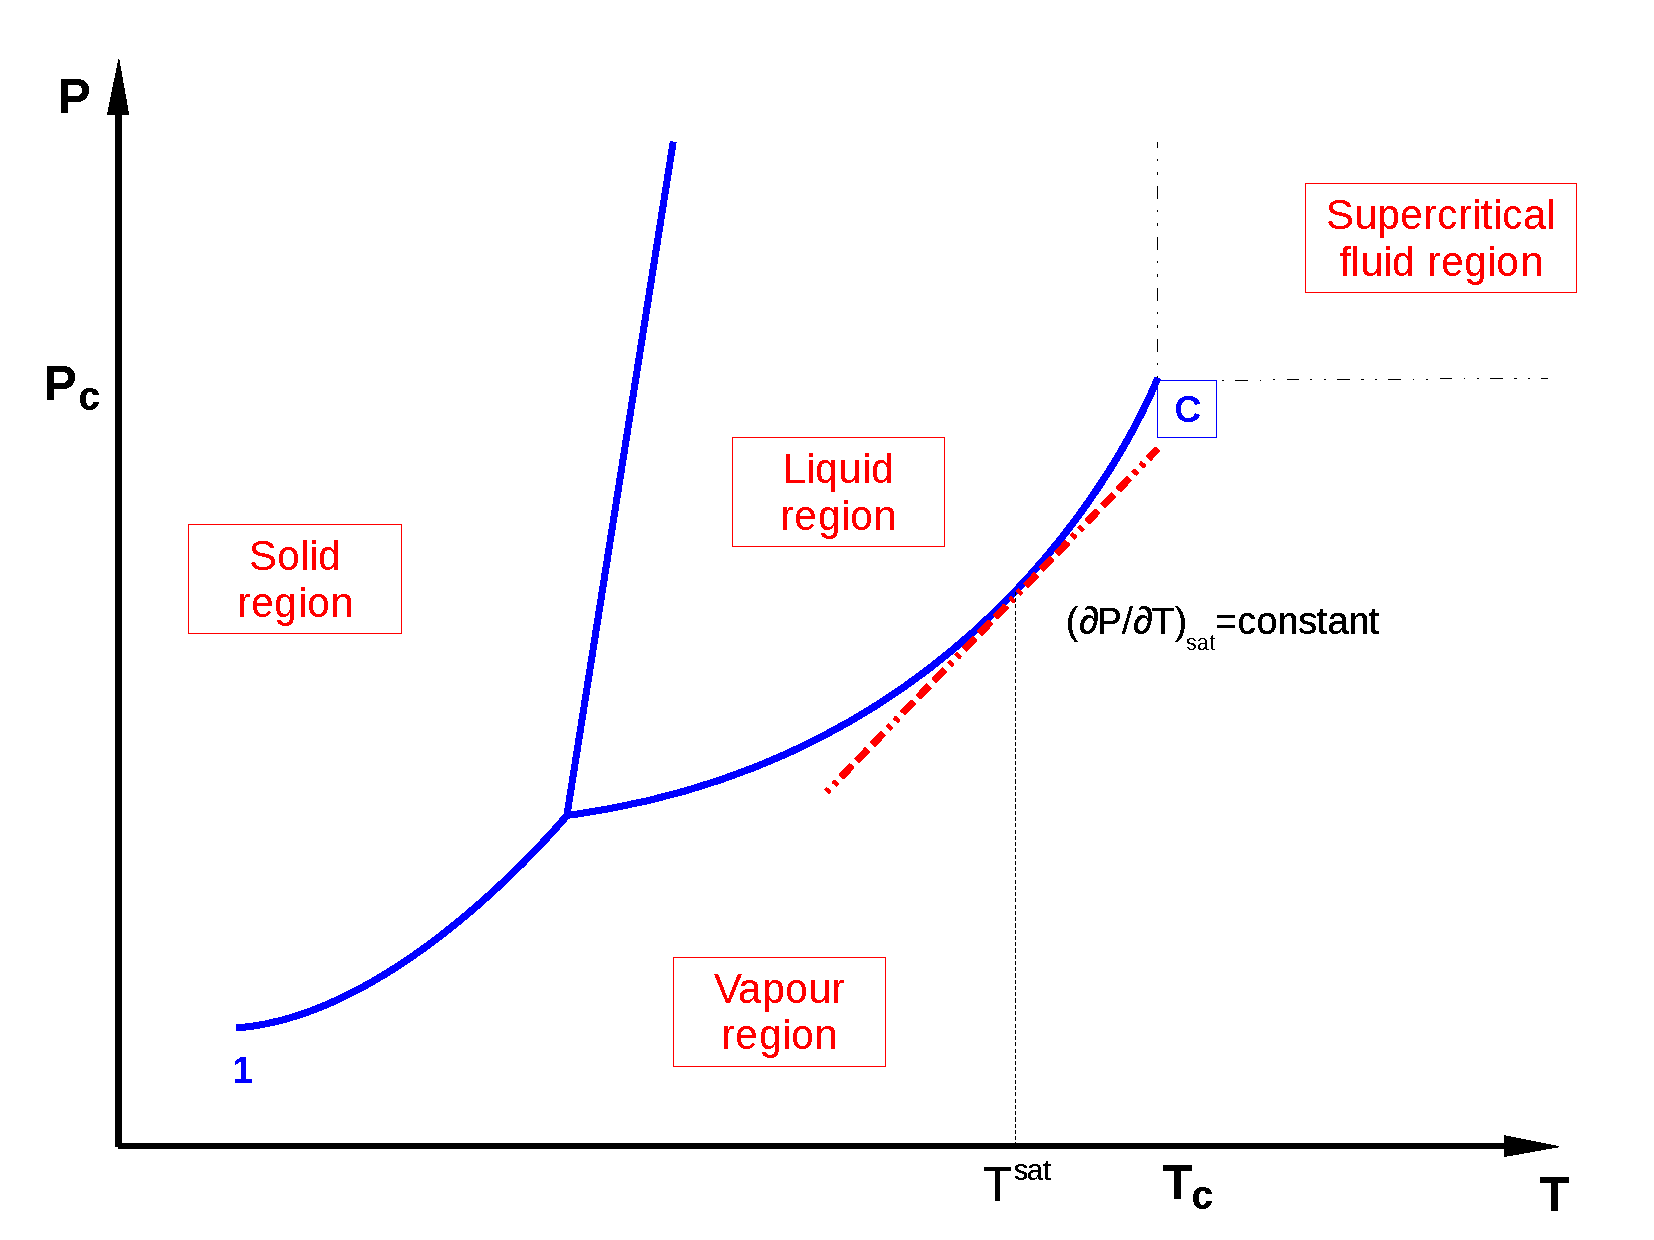
\includegraphics[width=.5\columnwidth,clip]{./../Pics/PT_Diagram2}
               \end{center} 
               \caption{ $PT$ diagrams for a pure substance. Graphical representation of the Clapeyron relation.}\label{Mod03Fig01}
           \end{figure}
      \begin{shaded}
          \begin{equation}
             \frc{d\left(\ln{P^{\text{sat}}}\right)}{dT} = \frc{\Delta H^{\text{fg}}}{RT^{2}} \;\;\Longrightarrow \;\;\; \ln{\left(\frc{P_{2}}{P_{1}}\right)_{\text{sat}}} = \frc{\Delta H^{\text{fg}}}{R}\left(\frc{1}{T_{1}}-\frc{1}{T_{2}}\right)_{\text{sat}}.\label{Mod03_ClausiusClapeyronEqn} 
          \end{equation} 
This expression is known as {\it Clausius-Clapeyron equation} and is a good approximation when describing temperature and pressure dependence at boiling/condensation and at sublimation/gas deposition.
      \end{shaded}
For the dependence of the saturated vapour pressure on $T$, a number of empirical relations have been developed. The simplest expression is,
    \begin{displaymath}
       \ln{P^{\text{sat}}} = A - \frc{B}{T},%\label{Mod03_AntoineSimplest}
    \end{displaymath}
where $A$ and $B$ are constants obtained from experiments. A more `popular' relation is,
    \begin{shaded}
       \begin{equation}
          \ln{P^{\text{sat}}} = A - \frc{B}{T+C},\label{Mod03_Antoine}
       \end{equation}
       this relation is known as {\it Antoine Equation}, where $A$, $B$ and $C$ are constants obtained experimentally.
    \end{shaded}
This two relations, although still widely used by the fluids community are plagued with strong inaccuracy. Due to better accuracy, high-order polynomial relations have become commonly used in flow and process simulators,
    \begin{displaymath}
       \ln{P^{\text{sat}}} = \frc{A\tau + B\tau^{1.5} + C\tau^{3} + D\tau^{6}}{1-\tau}\;\;\;\;\text{ with }\;\;\tau = 1 - T_{r}.
    \end{displaymath}
\end{subequations}


%%% SUBSECTION
   \subsection{Vapour-Liquid Equilibrium Systems}

Several processes of engineering relevance occur with fluids in phase equilibria -- either saturated vapour (\ie vapour saturated with liquid droplets) and saturated liquid (\ie liquid saturated with bubbles of vapour). In most cases, it is important to know the actual quantities of both phases in thermodynamic equilibrium, \ie the amount of vapour and liquid present in a constrained system at prescribed temperature and pressure conditions. Let assume that a closed system contains $n$ moles of a chemical species split into $\mathcal{P}$ phases,
    \begin{displaymath}
      n = \sum\limits_{j=1}^{\mathcal{P}} \mfr[n]{}{j} = \mfr[n]{}{1} + \mfr[n]{}{2} + \cdots + \mfr[n]{}{\mathcal{P}}.
    \end{displaymath}
The mass balance acroos all $\mathcal{P}$ phases can be represented as
    \begin{displaymath}
       nV = \mfr[n]{}{1}\mfr[V]{}{1} + \mfr[n]{}{2}\mfr[V]{}{2} + \cdots + \mfr[n]{}{\mathcal{P}}\mfr[V]{}{\mathcal{P}}  = \sum\limits_{j=1}^{\mathcal{P}}\left(nV\right)^{\left(j\right)},
    \end{displaymath}
where $V$ is the molar volume. Dividing by $n$
    \begin{displaymath}
       V = \frc{\mfr[n]{}{1}}{n}\mfr[V]{}{1} + \frc{\mfr[n]{}{2}}{n}\mfr[V]{}{2} + \cdots + \frc{\mfr[n]{}{\mathcal{P}}}{n}\mfr[V]{}{\mathcal{P}}.
    \end{displaymath}
Defining molar (or mole) fraction, $\mfr[x]{}{j}=\frc{\mfr[n]{}{j}}{n}$, where
    \begin{eqnarray}
         && \sum\limits_{j=1}^{\mathcal{P}}\mfr[x]{}{j} = 1,  \nonumber \\
         && V = \mfr[x]{}{1}\mfr[V]{}{1} + \mfr[x]{}{2}\mfr[V]{}{2} + \cdots + \mfr[x]{}{\mathcal{P}}\mfr[V]{}{\mathcal{P}}.  \nonumber
    \end{eqnarray}
For vapour-liquid systems,
    \begin{eqnarray}
         && \mfr[x]{}{L} + \mfr[x]{}{V} = 1,  \nonumber \\
         && V = \mfr[x]{}{L}\mfr[V]{}{L} + \mfr[x]{}{V}\mfr[V]{}{V}. \nonumber
    \end{eqnarray}
For a generic thermodynamic potential $M$ (= $V$, $U$, $H$, $S$ etc),
    \begin{shaded}
       \begin{subequations}
           \begin{equation}
              M = \left(1-\mfr[x]{}{V}\right)\mfr[M]{}{L} + \mfr[x]{}{V}\mfr[M]{}{V}
           \end{equation}
           \begin{equation}
              M = \mfr[M]{}{L} + \mfr[x]{}{V}\Delta\mfr[M]{}{LV}\label{Mod03_QualityVapour}
           \end{equation}
       \end{subequations}
    \end{shaded}
$\mfr[x]{}{V}$ is called \underline{\it vapour quality}. Thermodynamic potentials of pure substances are graphically represented by $Ph$ (pressure $\times$ specific enthalpy) and $Ts$ (temperature $\times$ specific entropy) diagrams, Fig.~\ref{Mod03Fig02}, where information on $P$, $T$, $s$, $h$, $x$ and $v$ (specific volume) can be readily extracted.
%
           \begin{figure}[h]
              \vbox{
                    \hbox{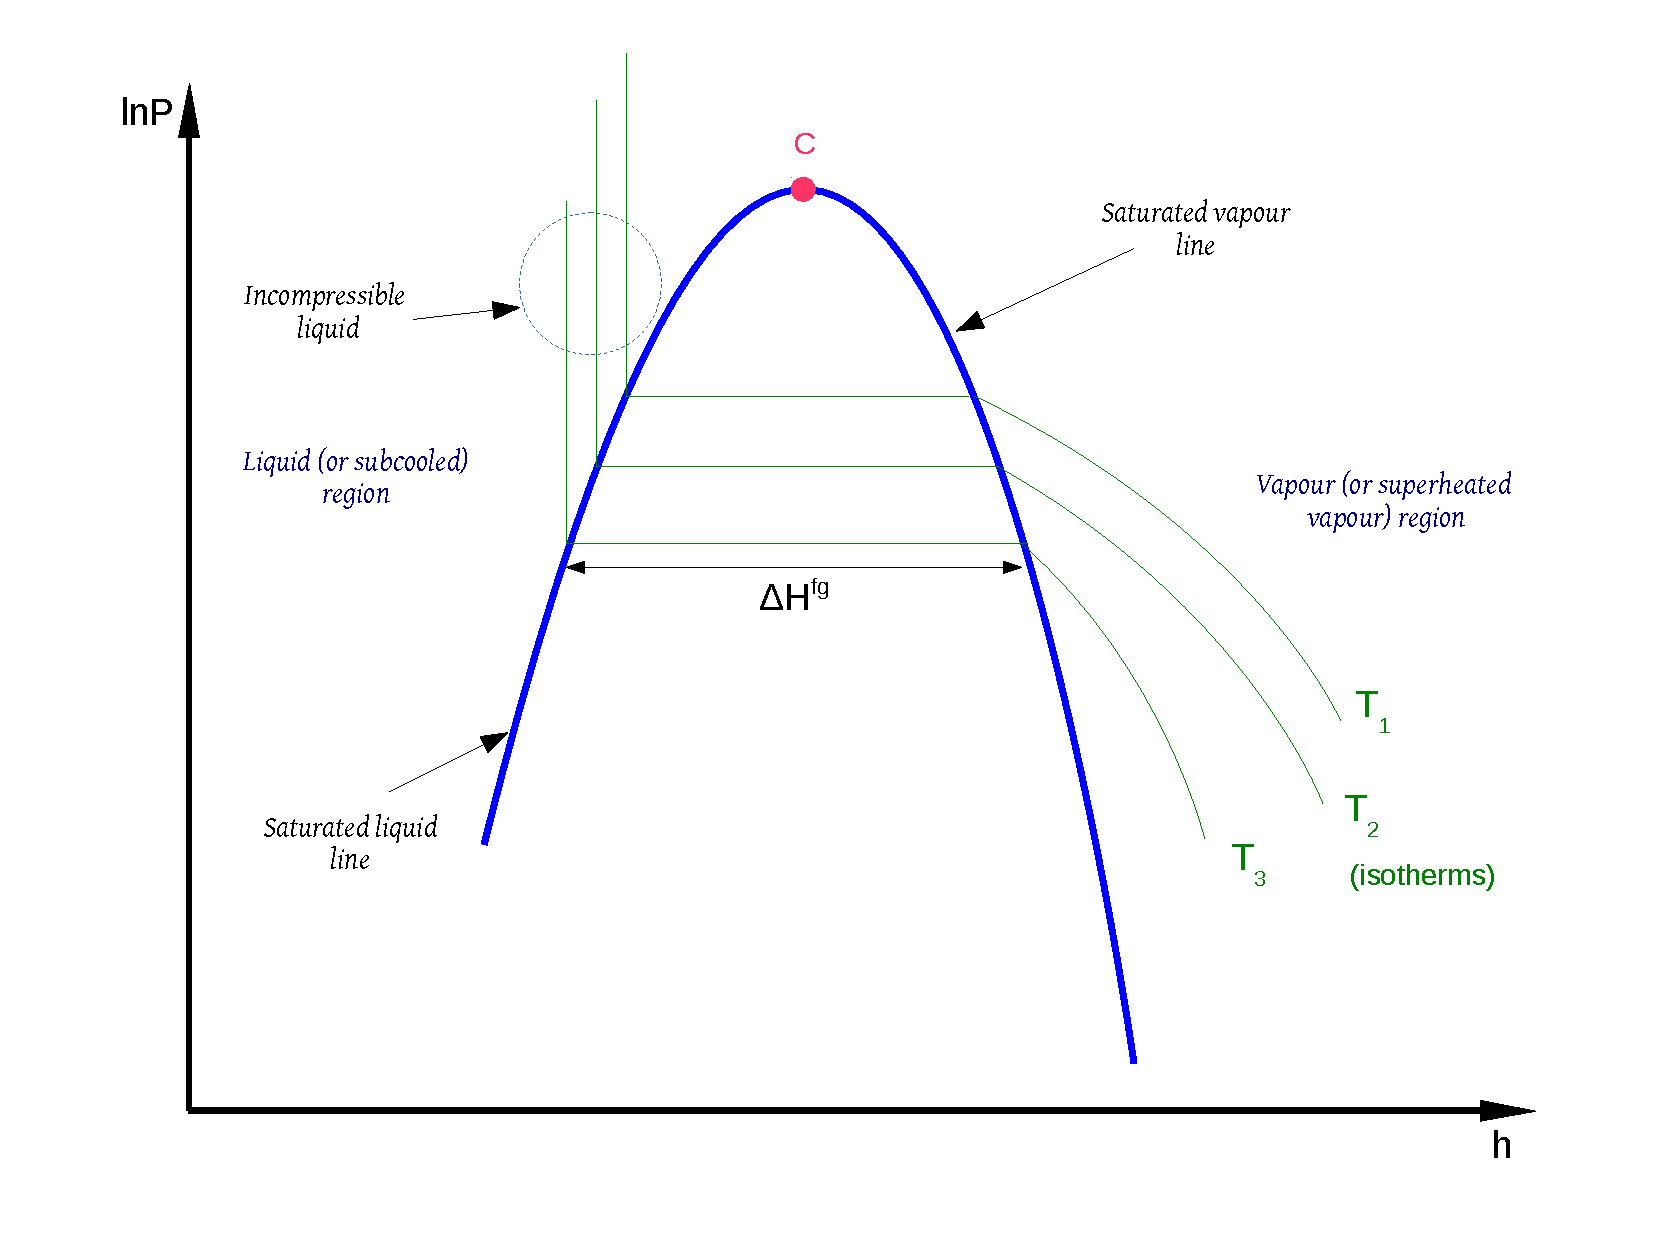
\includegraphics[width=.5\columnwidth,clip]{./Figs/Mod3PHDiagram}
                          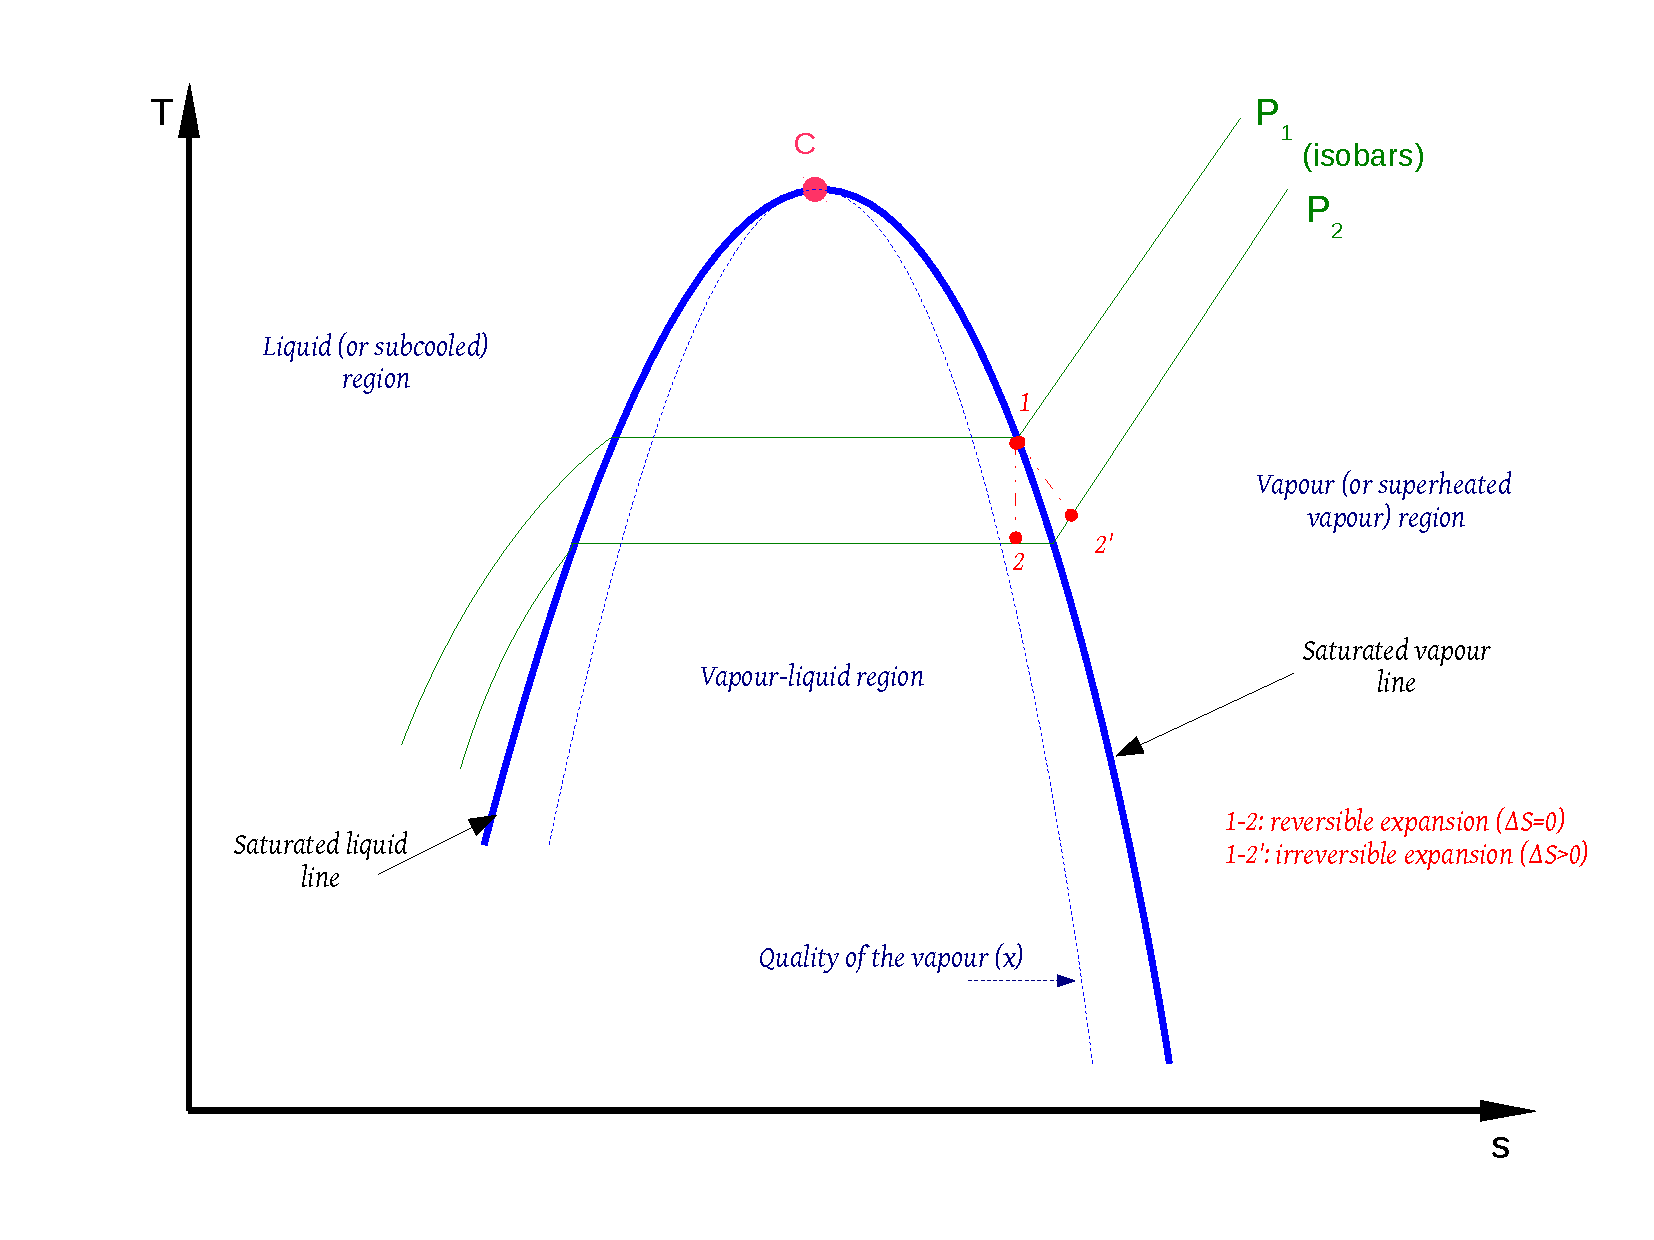
\includegraphics[width=.5\columnwidth,clip]{./Figs/Mod3TSDiagram}}
                    \vspace{-.1cm}
                    \hbox{\hspace{4cm}(a)\hspace{8cm}(b)}}
              \caption{ (a) $Ph$ and (b) $Ts$ diagrams for a pure substance.}\label{Mod03Fig02}
           \end{figure}
%
In the $Ph$ diagram, Fig~\ref{Mod03Fig02}a, isotherms (i.e., lines representing constant temperature) and pressure conditions determine the phase of the fluid. At the left hand-side of the {\it dome} all fluid is at liquid state, whereas at the right hand-side of the {\it dome}, all fluid is at vapour state. The region within the {\it dome} is a two-phase region, where liquid and vapour coexist in thermodynamic equilibrium. As the fluid conditions `move' from the {\it saturated liquid line} to the {\it saturated vapour line} through the {\it isotherm}, the fluid is continuously vaporised `till there is no droplets of liquid fluid. The total amount of heat given to the system -- $\Delta H^{\text{fg}}$, is the latent heat of vaporisation. In a similar way, the $Ts$ diagram, Fig~\ref{Mod03Fig02}b, shows similar features over different {\it isobars}. In addition, the {\it quality} of the vapour can also be graphically represented. In a reversible expansion from $P_{1}$ to $P_{2}$ $\left(P_{1}>P_{2}\right)$, entropy change is null, $\Delta s=0$, and is represented by a vertical line, however during irreversible expansion, $\Delta s >0$, represented by an inclined line.  

 $Ph$ and $Ts$ diagrams for common substances are no longer used by industry but it helps to qualitatively understand phase (and associated thermodynamic potentials) behaviour of pure substances. Quantitative information can be obtained from either saturated and superheated (Fig.~\ref{Mod03Fig03}) fluid tables or dedicated software, \eg
\begin{itemize}
   \item \href{http://www.weatherford.com/doc/wft183650}{PVTflex$^{TM}$};
   \item \href{http://www.kbcat.com/infochem-software/flow-assurance-software-multiflash/pvt-simulation}{Multiflash$^{TM}$};
   \item \href{https://www.honeywellprocess.com/en-US/explore/products/advanced-applications/unisim/Pages/default.aspx}{UniSim – Software for Process Design and Simulation};
   \item \href{http://webbook.nist.gov/chemistry/fluid/}{NIST Website}
   \item etc.
\end{itemize}
In general, table of {\it saturated fluid properties}, Fig.~\ref{Mod03Fig03}a, contains information of the fluid within the {\it dome}, whereas the table of {\it superheated fluid properties} refer to the region outside (rhs) the {\it dome}. 
%
   \begin{figure}[h]
      \vbox{
         \hbox{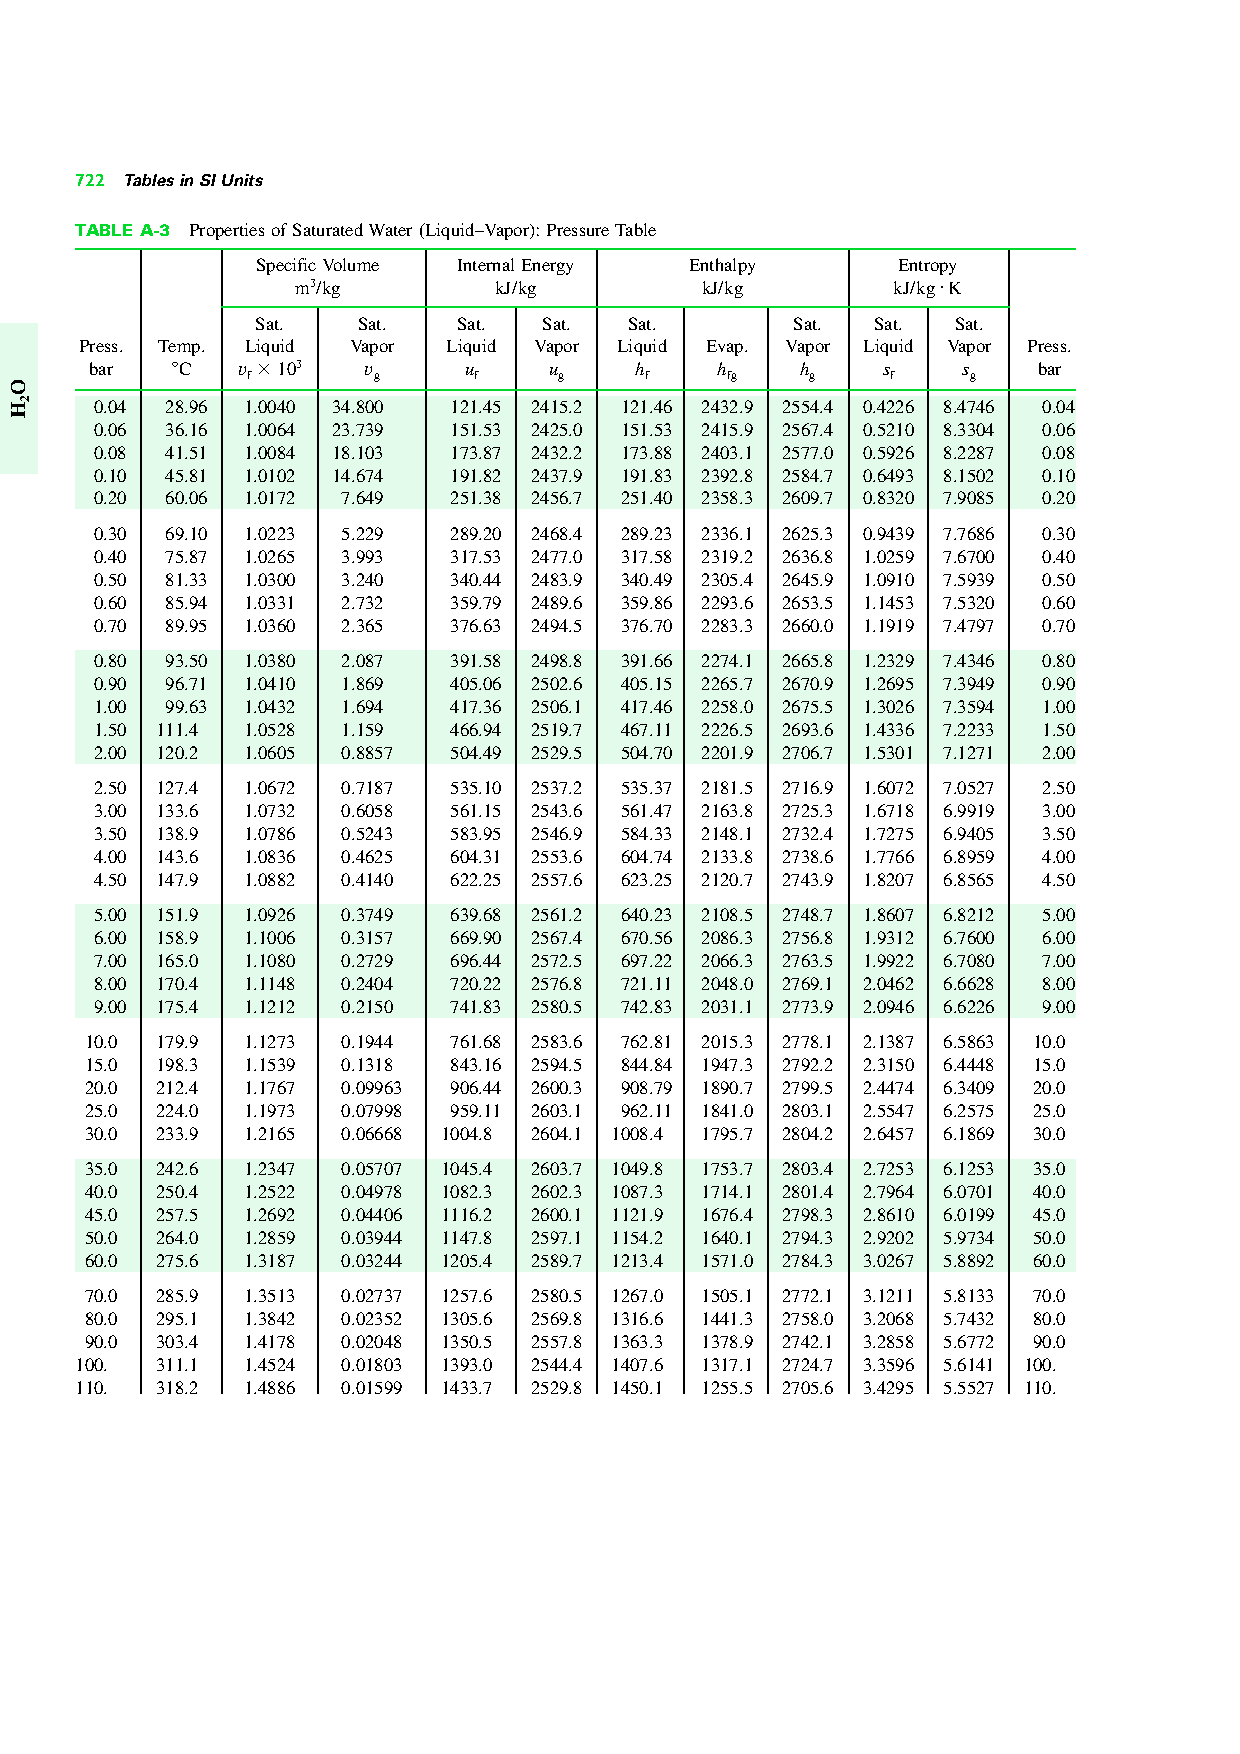
\includegraphics[width=.5\columnwidth,clip]{./Figs/WaterSatTable}
               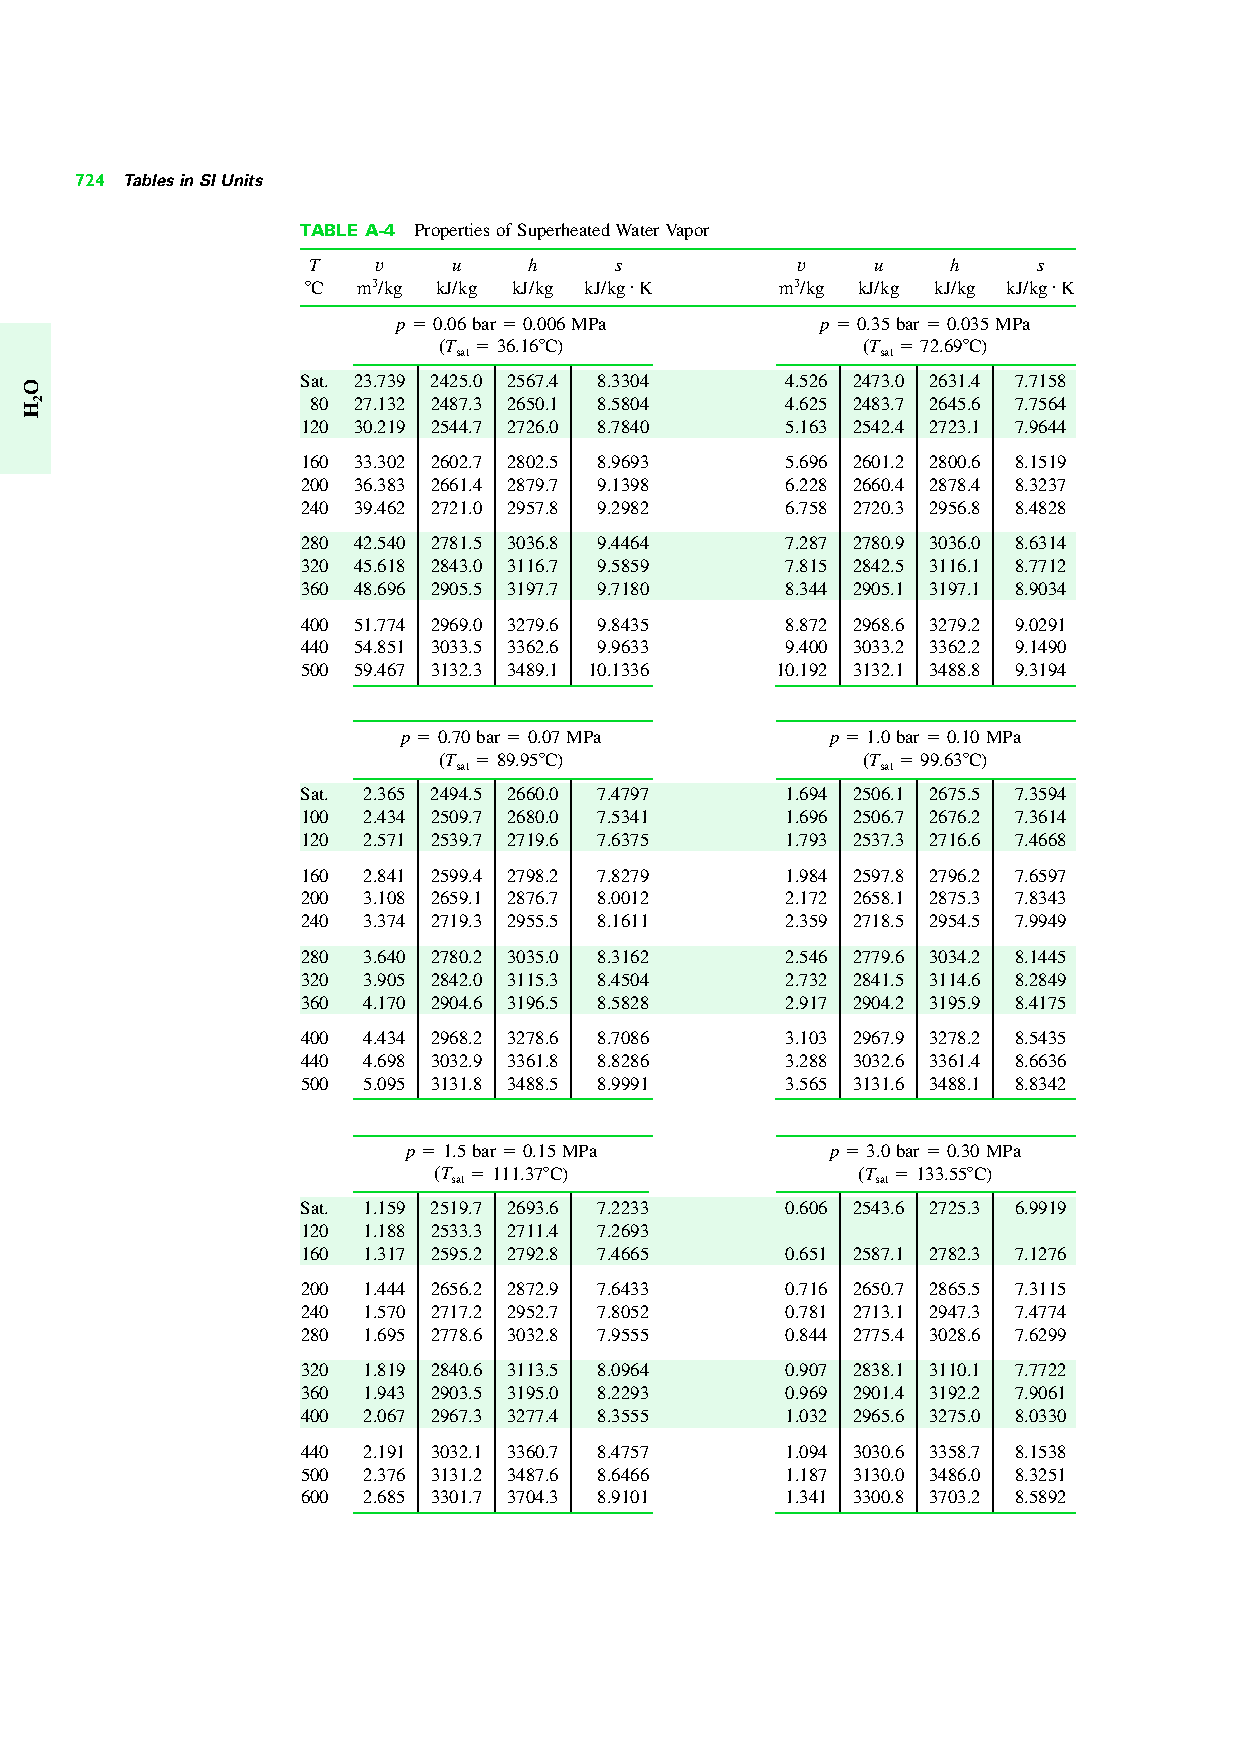
\includegraphics[width=.5\columnwidth,clip]{./Figs/Water_SuperheatedTable}}
         \vspace{-1.5cm}
         \hbox{\hspace{4cm}(a)\hspace{7cm}(b)}
      }
      \caption{ Table of properties of (a) saturated water-steam and (b) superheated vapour (Extracted from Moran $\&$ Saphiro, see Appendix B).}\label{Mod03Fig03}  
   \end{figure}
%
    

%%% SUBSECTION
   \subsection{Industrial Applications: Power System}
Regardless the energy source (fossil fuel, nuclear or geothermal), power plants are good applications for VLE systems as fluids are continuously vaporised and condensed by addition and extraction of heat and volume expansion. {\it Rankine thermal cycles} are system configurations for generating power and consist of four processes (Fig.~\ref{Mod03Fig04}) with associated energy balances:
     \begin{itemize}
      \item \textcolor{red}{Process 1-2}: reversible adiabatic (i.e., \blue{isentropic}) expansion in the turbine (or steam engine),
            \begin{displaymath}
               \left(h_{2} + \dot{W}_{T}\right)-h_{1} = 0 \Rightarrow \dot{W}_{T} = h_{1}-h_{2}
            \end{displaymath}
      \item \textcolor{red}{Process 2-3}: constant-pressure heat transfer (to the environment) in the condenser,
            \begin{displaymath}
               \left(h_{3} + \dot{Q}_{C}\right)-h_{2} = 0 \Rightarrow \dot{Q}_{C} = h_{2}-h_{3}
            \end{displaymath}
      \item \textcolor{red}{Process 3-4}: reversible adiabatic (i.e., \blue{isentropic}) pumping process in the feed pump,
            \begin{displaymath}
               h_{4} - \left(h_{3} + \dot{W}_{P}\right) = 0 \Rightarrow \dot{W}_{P} = h_{4}-h_{3}
            \end{displaymath}
      \item \textcolor{red}{Process 4-1}: constant-pressure heat transfer (to the fluid) in the boiler,
            \begin{displaymath}
               h_{1} - \left(h_{4} + \dot{Q}_{B}\right) = 0 \Rightarrow \dot{Q}_{B} = h_{1}-h_{4}
            \end{displaymath} 
     \end{itemize}
     The efficiency $\left(\eta\right)$ of the Rankine cycle is given by
           \begin{displaymath}
               \eta_{\text{Rankine}} = \frc{\sum W_{i}}{Q_{B}} = \frc{\left|W_{\text{net}}\right|}{Q_{B}} = \frc{\left|\left(h_{1}-h_{2}\right)+\left(h_{4}-h_{3}\right)\right|}{h_{1}-h_{4}}.
           \end{displaymath}
     Due to engineering constraints, fluids entering and leaving the pump \underline{must be} at liquid phase, thus $h_{4}=h_{f4}$ and $h_{3}=h_{f3}$, \ie the fluid has the enthalpy of the liquid phase (from the saturated fluid table) at the prescribed temperature and pressure conditions. {\it Pumps} are able to induce the transport of liquid fluids that are often assumed incompressible, therefore
          \begin{displaymath}
                Tds = dh - v dP
          \end{displaymath}
as the compression occurs isentropically, \ie $ds=0$,
          \begin{displaymath}
                dh = v dP \Rightarrow h_{f4} = h_{f3} + v_{3}\left(P_{4}-P_{3}\right).
          \end{displaymath}
However, as $\left(h_{f4}-h_{f3}\right) <<<<< \left(h_{1}-h_{2}\right)$, the efficiency can be considered as
           \begin{displaymath}
               \eta_{\text{Rankine}} = \frc{\left|\left(h_{1}-h_{2}\right)\right|}{h_{1}-h_{f4}}.
           \end{displaymath}     
%
   \begin{figure}[h]
      \begin{center}
         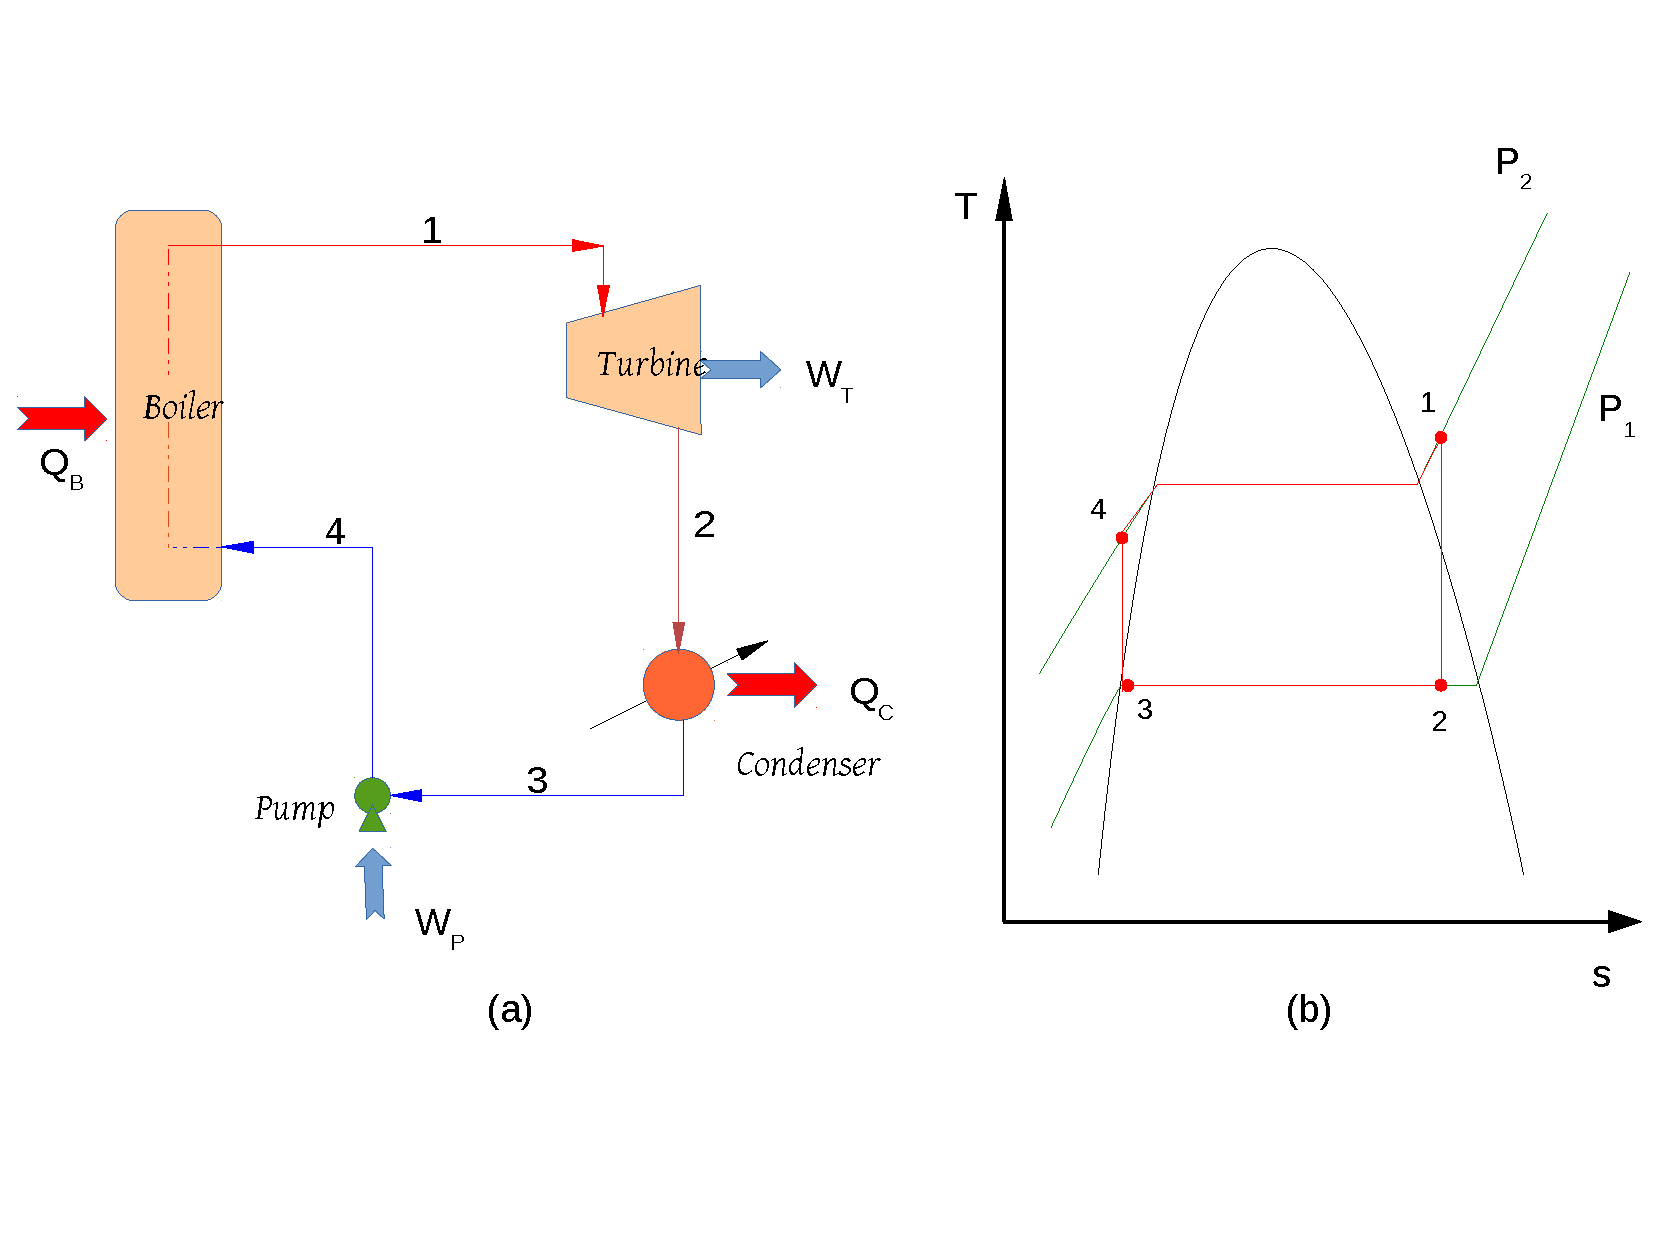
\includegraphics[width=\columnwidth,clip]{./Figs/Mod3PowerSystemDiagram}
      \end{center}
      \caption{ (a) Diagram of Rankine thermal cycle for power generation and associated $Ts$ diagram.}\label{Mod03Fig04}
   \end{figure}


\clearpage

%%% SECTION
\section{Examples}
       \begin{enumerate}

%%%
%%% EXAMPLE 
%%%
\item\label{Mod03Ex03} The Antoine equation constants for toluene are $A=14.01415$, $B=3106.46$ K and $C=-53.15$ K (for pressure given in kPa). At 1.01325$\times$10$^{5}$ Pa, calculate the boiling temperature and the enthalpy of vaporisation at this temperature.

% SOLUTION
    \noindent{\bf Solution:} Boiling temperature can be calculated from the Antoine equation,
       \begin{displaymath}
          \ln{P^{\text{sat}}} = A - \frc{B}{T+C} \;\;\;\Rightarrow \;\;\; T = \frc{B}{A-\ln{P^{\text{sat}}}} - C = \red{383.77 K}
       \end{displaymath}
The enthalpy of vaporisation, $\Delta H^{\text{fg}}$, can be obtained from the Clausius-Clapeyron equation,
         \begin{eqnarray}
            \frc{d}{dT} \left(\ln{P^{\text{sat}}}\right) &=& \frc{\Delta H^{\text{fg}}}{RT^{2}} \nonumber \\
             \frc{B}{\left(T+C\right)^{2}} &=&  \frc{\Delta H^{\text{fg}}}{RT^{2}} \;\;\Longrightarrow \Delta H^{\text{fg}} = 34.7984 \text{kJ.mol}^{-1}. \nonumber
         \end{eqnarray}
 
\clearpage

%%%
%%% EXAMPLE 
%%%  
\item\label{Mod03Ex04} Derive an expression for enthalpy change of a gas during an isothermal process assuming using the following EOS: $P\left(V-b\right)=RT$

% SOLUTION
    \noindent{\bf Solution:} We have seen that enthalpy change is given by Eqn.~\ref{Chapter:ThermodynamicPropertiesPureFluids:Eqn:DerivedEnthalpyRelation1},
    \begin{displaymath}
       dH = C_{p}dT + \left[V - T\Partial[V]{T}{P}\right]dP.
    \end{displaymath}
    We can rearrange the given EOS and obtain $\Partial[V]{T}{P}$,
    \begin{eqnarray}
       && P\left(V-b\right)=RT \;\;\;\rightarrow\;\;\; V = \frc{RT}{P} + b \;\;\;\rightarrow\;\;\; \Partial[V]{T}{P} = \frc{R}{P}\;\;\text{ thus, } \nonumber \\
       && dH = C_{p}dT + \left(V - \frc{RT}{P}\right)dP = \blue{C_{p}dT + bdP}. \nonumber 
    \end{eqnarray}
    
\clearpage
    
\clearpage
 
%%%
%%% EXAMPLE 
%%%  
\item\label{Mod03Ex06} Steam (dry and saturated) is supplied by the boiler at 15 bar and the condenser inlet pressure is 0.4 bar. Calculate the Rankine efficiency of the cycle. Neglect the pump work, assume the enthalpy of fluid leaving the pump is 317.58 kJ.kg$^{-1}$

% SOLUTION  
    \noindent{\bf Solution:} At 15 bar, dry and saturated $\left(\ie x_{1}=1\right)$ steam has the following properties (from saturated table)\footnote{Using the same numbering as in Fig.~\ref{Mod03Fig04}.},
          \begin{eqnarray}
             T_{1} &=& T_{\text{sat}} = 198.3^{\circ}\text{C},\nonumber \\
             h_{1} &=& h_{\text{g}} = 2792.2\; \text{kJ.kg}^{-1} \nonumber \\
             s_{1} &=& s_{\text{g}} = 6.4448\; \text{kJ.(kg.K)}^{-1} \nonumber
          \end{eqnarray} 
    In the condenser, $P_{2}=0.4$ bar,
          \begin{eqnarray}
              T_{2} &=& T_{\text{sat}} = 75.87^{\circ}\text{C}, \nonumber \\
              h_{\text{g}2} &=& 2636.8\;\text{kJ.kg}^{-1},\;\;\; h_{\text{f}2} = 317.58\;\text{kJ.kg}^{-1},  \nonumber \\
              s_{\text{g}2} &=& 7.6700 \;\text{kJ.(kg.K)}^{-1},\;\;\; s_{\text{f}2} = 1.0259\;\text{kJ.(kg.K)}^{-1}. \nonumber  
          \end{eqnarray}
$h_{2}$ and $s_{2}$ depend on the knowledge of how vaporised the water is, in other words, we need to determine the quality of the steam, $x_{1}$ through Eqn.~\ref{Mod03_QualityVapour},
      \begin{eqnarray}
          h_{2} &=& h_{\text{f}2} + x_{2}\left(h_{\text{g}2} - h_{\text{f}2}\right), \nonumber \\
          s_{2} &=& s_{\text{f}2} + x_{2}\left(s_{\text{g}2} - s_{\text{f}2}\right). \nonumber
      \end{eqnarray}
As we know that water is expanded isentropically in the turbine, \ie $s_{1}=s_{2}$,
      \begin{displaymath}
         s_{2} = s_{\text{f}2} + x_{2}\left(s_{\text{g}2} - s_{\text{f}2}\right) = s_{1} = 6.4448 \;\;\;\Rightarrow \;\;\; x_{2} = 0.8156 \;\;(81.56\% \text{ of vapour}
      \end{displaymath}
Thus replacing in 
      \begin{displaymath}
          h_{2} = h_{\text{f}2} + x_{2}\left(h_{\text{g}2} - h_{\text{f}2}\right) = 2209.14\text{ kJ.kg}^{-1}.
      \end{displaymath}
The Rankine efficiency is given by
      \begin{displaymath}
           \eta_{\text{Rankine}} = \frc{\text{Adiabatic or Isentropic Heat Drop}}{\text{Heat Supplied}} = \frc{\left|h_{1}-h_{2}\right|}{h_{1}-h_{\text{f}4}} = 0.2356\;\;\;\rightarrow \;\;\; 23.56\%
      \end{displaymath}
    


\end{enumerate}


 % Thermodynamic Properties of Pure Fluids 

\part{Power and Refrigeration Systems}

\part{Porous Media Flows}

%\part{Power and Refrigeration}

\pagebreak

\cleardoublepage

  \begin{appendix}
     \part{Appendices} 
         \setcounter{examplecounter}{0}
       
\chapter{Physical Constants and Conversion Factors}\label{Chapter:UnitConversion}

%%% SECTION
\section{Gas Contant, $R$}\label{Chapter:UnitConversion:Section:GasConstant}
     \begin{center}
     \begin{tabular}{|c c|}
       \hline
           $\mathbf{R}$   & {\bf Units} $\mathbf{\left(\text{V.P.T}^{-1}\text{n}^{-1}\right)}$ \\
           \hline\hline
           8.3145    &  J.K$^{-1}$.mol$^{-1}$  \\
           8.3145    &  kJ.K$^{-1}$.kmol$^{-1}$  \\
           8.3145    &  l.kPa.K$^{-1}$.mol$^{-1}$  \\
           8.3145$\times$10$^{-3}$    & cm$^{3}$.kPa.K$^{-1}$.mol$^{-1}$  \\
           8.3145    &  m$^{3}$.Pa.K$^{-1}$.mol$^{-1}$  \\
           8.3145$\times$10$^{-5}$    &  m$^{3}$.bar.K$^{-1}$.mol$^{-1}$  \\
           8.2057$\times$10$^{-2}$ &  l.atm.K$^{-1}$.mol$^{-1}$  \\
           \hline         
     \end{tabular}
     \end{center}
     
%%% SECTION
\section{Length}\label{Chapter:UnitConversion:Section:Length}
     \begin{center}
     \begin{tabular}{|l l l l l|}
       \hline
       1 m =& 3.2808 ft =& 39.37 in =& 10$^{2}$ cm =& 10$^{10}$ A \\
       1 mm =& 10$^{-3}$ m =& 10$^{-1}$ cm =& 10$^{-6}$ km &       \\
       1 mile =& 5280 ft =& 1609.36 m =& 1.609 km &             \\
       \hline           
     \end{tabular}
     \end{center}
          
%%% SECTION
\section{Area}\label{Chapter:UnitConversion:Section:Area}
     \begin{center}
     \begin{tabular}{|l l l l l|}
       \hline
       1 m$^{2}$ =& 10$^{4}$ cm$^{2}$ =& 10.76 ft$^{2}$ =& 1550 in$^{2}$ & \\
       1 in$^{2}$ =& 6.944$\times$10$^{-3}$ ft$^{2}$ =& 6.4516$\times$10$^{-4}$ m$^{2}$ & & \\
       \hline           
     \end{tabular}
     \end{center}
          
%%% SECTION
\section{Volume}\label{Chapter:UnitConversion:Section:Volume}
     \begin{center}
     \begin{tabular}{|l l l l l|}
       \hline    
       1 m$^{3}$ =& 35.313 ft$^{3}$ =& 6.1023$\times$10$^{4}$ in$^{2}$ =& 1000 l =& 264.171 gal \\
       \hline            
     \end{tabular}
     \end{center}
          
%%% SECTION
\section{Mass}\label{Chapter:UnitConversion:Section:Mass}
     \begin{center}
     \begin{tabular}{|l l l l l|}
       \hline    
        1 kg =& 1000 g =& 2.2046 lbm & & \\
       \hline            
     \end{tabular}
     \end{center}


          
%%% SECTION
\section{Force}\label{Chapter:UnitConversion:Section:Force}
     \begin{center}
     \begin{tabular}{|l l l l l|}
       \hline    
         1 N =& 10$^{5}$ dyne =& 1 kg.m.s$^{-2}$ =& 0.225 lbf & \\
       \hline            
     \end{tabular}
     \end{center}

     
%%% SECTION
\section{Energy}\label{Chapter:UnitConversion:Section:Energy}
     \begin{center}
     \begin{tabular}{|l l l l l|}
       \hline
       1 J =& 1 N.m  =& 1 kg.m$^{2}$.s$^{-2}$ =& 9.479$\times$10$^{-4}$ Btu &  \\
       1 kJ =&  1000 J  =&  0.9479 Btu  =& 238.9 cal &                      \\
       \hline           
     \end{tabular}
     \end{center}
     
%%% SECTION
\section{Power}\label{Chapter:UnitConversion:Section:Power}
     \begin{center}
     \begin{tabular}{|l l l l l|}
       \hline
       1 W =& 1 J.s$^{-1}$  =& 1 kg.m$^{2}$.s$^{-3}$ =& 3.412 Btu.h$^{-1}$ =& 1.3405$\times$10$^{-3}$ hp   \\
       1 kW =&  1000 W  =& 3412 Btu.h$^{-1}$  =& 737.3 ft.lbf.s$^{-1}$ =& 1.3405 hp  \\
       \hline           
     \end{tabular}
     \end{center}
     
%%% SECTION
\section{Pressure}\label{Chapter:UnitConversion:Section:Pressure}
     \begin{center}
     \begin{tabular}{|l l l l l|}
       \hline
       1 Pa =& 1 N.m$^{-2}$ =& 1 kg.m$^{-1}$.s$^{-2}$ =& 1.4504$\times$10$^{-4}$ lbf.in$^{-2}$ & \\
       1 atm =& 14.696 lbf.in$^{-2}$ =& 1.01325$\times$10$^{5}$ Pa =& 101.325 kPa =& 760 mm-Hg \\
       1 dyne.cm$^{-2}$ =& 0.1 Pa =& 10$^{-6}$ bar =& 145.04 lbf.in$^{-2}$ & \\
       1 bar =& 10$^{5}$ Pa =& 0.987 atm =& 14.504 lbf.in$^{-2}$ & \\
       \hline           
     \end{tabular}
     \end{center}
     
%%% SECTION
     \section{Temperature}\label{Chapter:UnitConversion:Section:Temperature}
     \begin{displaymath}
       \begin{cases}
         T\left(^{\circ}F\right) = \frc{9}{5}T\left(^{\circ}C\right) + 32 = T(R) - 459.67 & \\
         T\left(^{\circ}C\right) = \frc{5}{9}\left[T\left(^{\circ}C\right)-32\right] = T(K) - 273.15 & 
       \end{cases}      
     \end{displaymath}
     
%%% SECTION
     \section{Viscosty}\label{Chapter:UnitConversion:Section:Viscosity}
     \begin{center}
     \begin{tabular}{|l l l l l|}
       \hline
       1 Pa.s =& 1 N.s.m$^{-2}$ =& 1 kg.m$^{-1}$.s$^{-1}$ =& 10 poise &   \\
       1 poise =& 1 dyne.s.cm$^{-2}$ =& 1 g.cm$^{-1}$.s$^{-1}$ =& 0.1 Pa.s =& 6.72$\times$10$^{-2}$ lbm.ft$^{-1}$.s$^{-1}$\\
       1 stoke =& 1 cm$^{2}$.s$^{-1}$ =& 10$^{-4}$cm$^{2}$.s$^{-1}$ =& 1.076$\times$10$^{-3}$ ft$^{2}$.s$^{-1}$ & \\
       \hline           
     \end{tabular}
     \end{center}
     
    
  % Example
  \begin{MyExample}{\begin{center}{\bf Example}\end{center}}
       %
     \begin{example}\label{Chapter:UnitConversion:Example1}
       Calculate the volume $\left(\text{in m}^{3}\right)$ of 1 kg of hydrogen gas $\left(\text{molecular mass of 2.016 kg.kgmol}^{-1}\right)$ at 27$^{\circ}$C and 1 bar. Assume ideal gas behaviour.
     \end{example}

     % SOLUTION
     \noindent We can use the ideal gas equation of state to calculate the volume of H$_{2}$ gas,
           \begin{displaymath}
              V = \frc{nRT}{P},
           \end{displaymath}
           where $n = m/MW$ is the number of moles, $m$, $MW$ and $R$ are the mass, molecular mass, and universal gas constant, respectively. We should be able to replace the variables with their values,
           \begin{eqnarray}
              V &=& \frc{nRT}{P} = \frc{ \frc{m}{MW} R T }{ P } \nonumber \\
                &=& \frc{ \frc{ 1\text{ kg}}{ 2.016\text{ kg.kgmol}^{-1}}\;\; 0.08314\frc{\text{bar.m}^{3}}{\text{kgmol.K}}\;\; ( 27 + 273.15)\text{ K}}{ 1 \text{ bar}},\nonumber
           \end{eqnarray}
           It is clear that the units above are consistent and can be easily eliminated resulting in m$^{3}$,
           \begin{eqnarray}
              V &=& \frc{ \frc{ 1\cancel{\text{ kg}}}{ 2.016\text{ \cancel{kg}.}\cancel{\text{kgmol}^{-1}}}\;\; 0.08314\frc{\text{\cancel{bar}.m}^{3}}{\text{\cancel{kgmol}.\cancel{K}}}\;\; ( 27 + 273.15)\cancel{\text{ K}}}{ 1 \text{ \cancel{bar}}},\nonumber \\
                &=& 12.3782\text{ m}^{3}.\nonumber
           \end{eqnarray}
     %
       \begin{example}\label{Chapter:UnitConversion:Example2}
              Liquid water at 0.70 bar is transferred from a condenser to a boiler through a pump. The pressure in the exit of the pump is 25 bar. Assuming that the water undertakes an isentropic (\ie constant entropy) compression, calculate the specific enthalpy of the water after the pump. Consider that the liquid water as incompressible and
          \begin{displaymath}
            dh = Tds + vdP,
         \end{displaymath}
         where h, s, v are specific enthalpy (kJ/kg), entropy (kJ/(kg.K)) and volume (m$^{3}$.kg).
     \end{example}

     % SOLUTION
     \noindent If the process is isentropic, therefore $ds=0$ and the fundamental thermodynamic relation is simplified to,
       \begin{displaymath}
          dh = vdP \Longrightarrow h_{2} - h_{1} = v\left(P_{2}-P_{1}\right),
       \end{displaymath}
      or summarising,
       \begin{center}
         \begin{tabular}{c| c c c}
            State  & $P$ (bar)  & $h$ (kJ/kg) & $v$ $\left(\text{m}^{3}\text{.kg}\right)$ \\
\hline
              1    &   0.70    &  376.70   &  1.0360$\times$10$^{-3}$                 \\
              2    &  25.0    & \red{h$_{2}$}& 1.0360$\times$10$^{-3}$ 
         \end{tabular}
       \end{center}
       Values of {\it State 1} were obtained from the water saturated table (Appendix~\ref{Appendix:Saturated_SH_Tables}). Note that as the fluid is assumed incompressible there is no variation in the volume, $v_{1}=v_{2}$.
       \begin{eqnarray}
         h_{2} &=& h_{1} = v\left(P_{2}-P_{1}\right) \nonumber \\
              &=& 376.70\frc{\text{kJ}}{\text{kg}} + 1.0360\times 10^{-3}\frc{\text{m}^{3}}{\text{kg}}\;\left(25 - 0.70\right)\text{ bar}  \nonumber\\
              &=& 376.70\frc{\text{kJ}}{\text{kg}} + 0.02517 \frc{\text{m}^{3}.\text{bar}}{\text{kg}} \nonumber
       \end{eqnarray}
       It is clear that the units in the two terms of the r.h.s. of the equation contain distinct units that \underline{can not} be summed up. Therefore, we need to convert $\left[\text{m}^{3}.\text{bar}\right]$ to $[\text{kJ}]$. Bearing in mind that 1 J = 1 N.m = 1 kg.m$^{2}$.s$^{-2}$, we first can convert $\left[\text{m}^{3}.\text{bar}\right]$ to $\left[\text{kg.m}^{2}.\text{s}^{-2}\right]$
       \begin{displaymath}
          1 \cancelto{\blue{\text{m}^{2}}}{\text{m}^{3}}.\red{\cancel{\text{bar}}} \times \frc{\red{10^{5}\cancel{\text{ Pa}}}}{\red{1 \cancel{\text{ bar}}}} \times \frc{\red{ 1 \text{ kg}/\left(\cancel{\blue{\text{m}}}.\text{s}^{2}\right)}}{\red{ 1 \cancel{\text{ Pa}}}} = 10^{5} \frac{\text{kg.m}^{2}}{\text{s}^{2}}
       \end{displaymath}
       Now, replacing the converted $\left[\text{m}^{3}.\text{bar}\right]$ term in the r.h.s. of the expression for $h_{2}$,
       \begin{eqnarray}
         h_{2} &=& 376.70\frc{\text{kJ}}{\text{kg}} + 0.02517 \frc{\text{m}^{3}.\text{bar}}{\text{kg}} \nonumber \\
              &=& 376.70\frc{\text{kJ}}{\text{kg}} + 0.02517 \frc{\cancel{\left(\text{m}^{3}.\text{bar}\right)}}{\text{kg}} \times \frc{10^{5} \frac{\text{kg.m}^{2}}{\text{s}^{2}}}{1 \cancel{\left(\text{m}^{3}.\text{bar}\right)}} \nonumber \\
              &=& 376.70\frc{\text{kJ}}{\text{kg}} + 2517 \frc{\cancelto{\red{\text{J}}}{\frac{\text{kg.m}^{2}}{\text{s}^{2}}}}{\text{kg}}\nonumber\\
              &=& 376.70\frc{\text{kJ}}{\text{kg}} + 2517 \frc{\text{J}}{\text{kg}} \nonumber
       \end{eqnarray}
       We still \underline{can not} sum the two terms in the r.h.s., as the first term involves $\left[\text{kJ/kg}\right]$ whereas the second term is $\left[\text{J/kg}\right]$, therefore
       \begin{eqnarray}
         h_{2} &=& 376.70\frc{\text{kJ}}{\text{kg}} + 2517 \frc{\text{J}}{\text{kg}} \nonumber\\
              &=& 376.70\frc{\text{kJ}}{\text{kg}} + 2517 \frc{\cancel{\text{J}}}{\text{kg}} \red{\times \frc{1\text{ kJ}}{1000 \cancel{\text{J}}}}\nonumber\\
              &=& 379.22 \frc{\text{kJ}}{\text{kg}}\nonumber
       \end{eqnarray}
     %

   \end{MyExample}
   

  %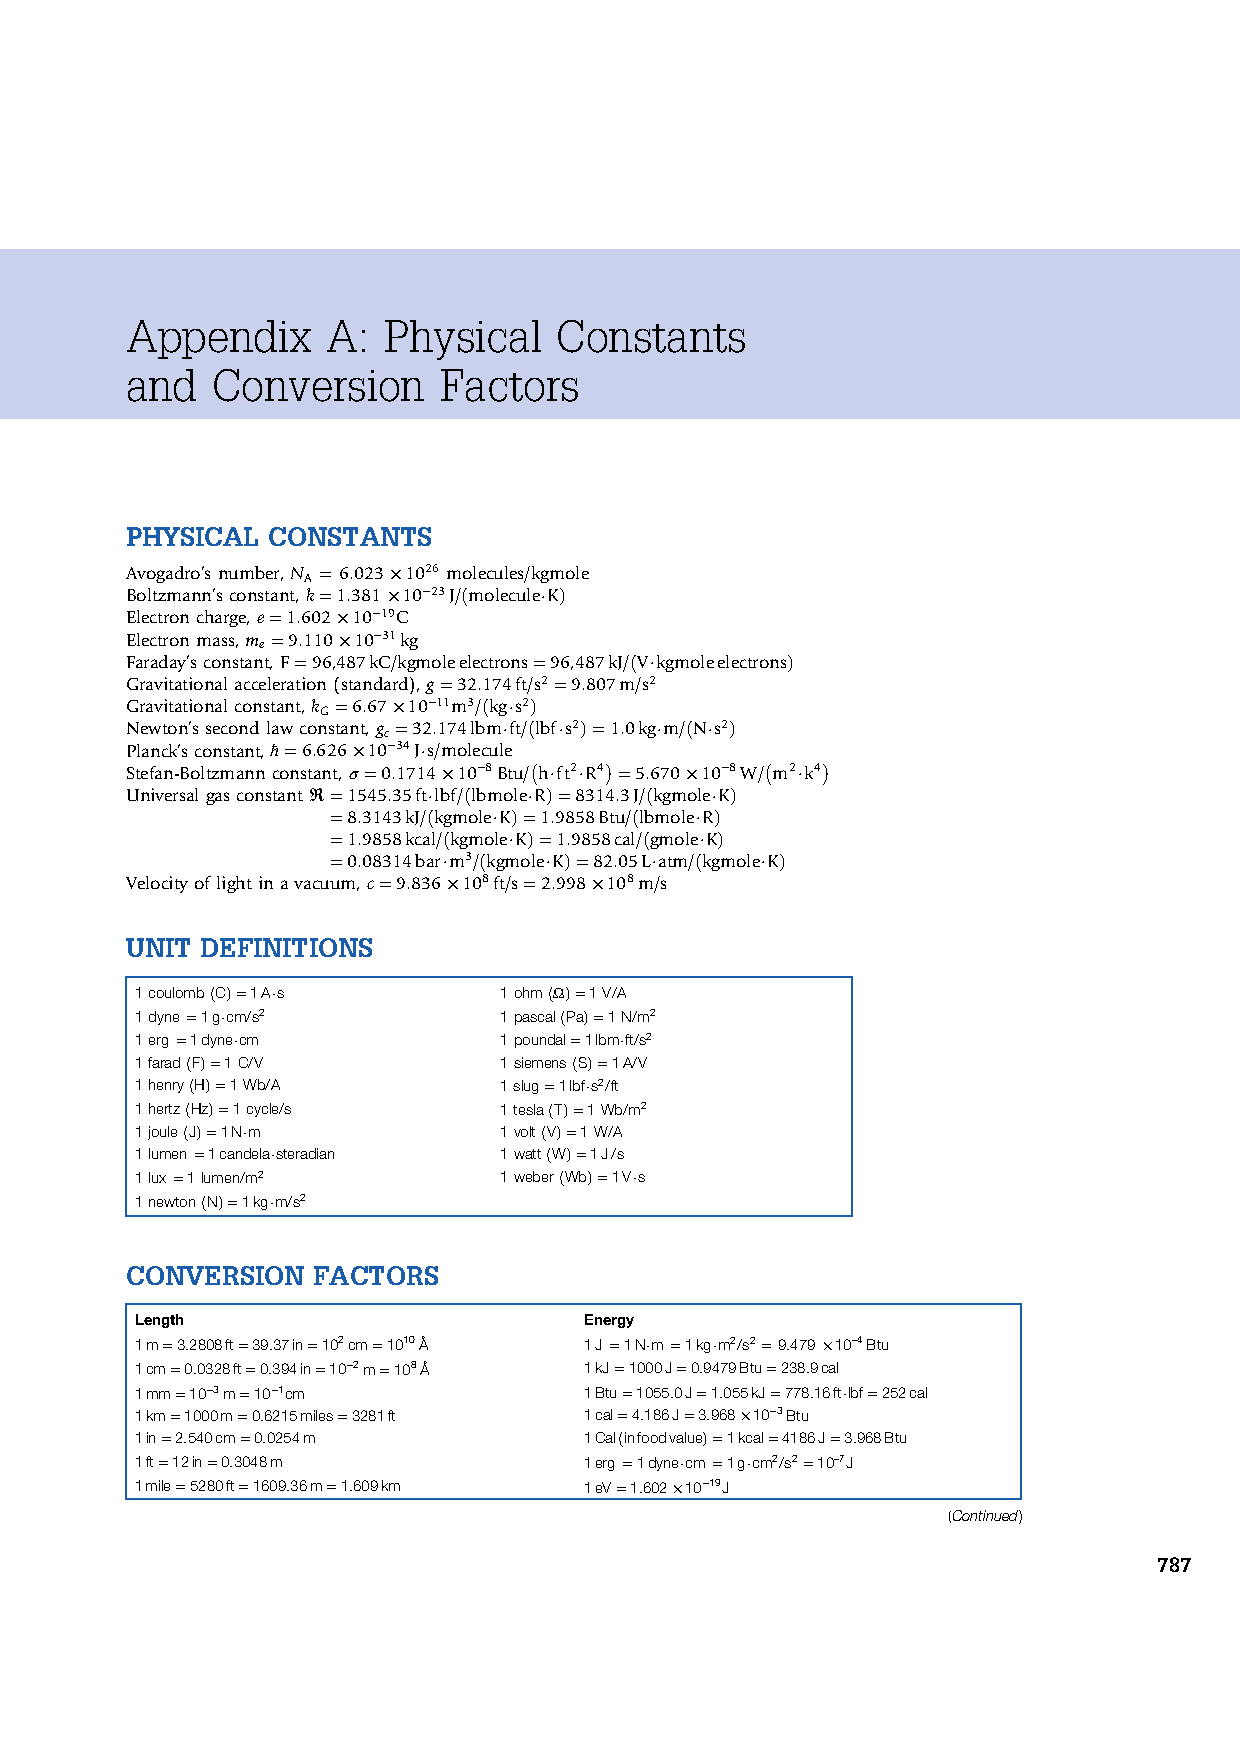
\includepdf[scale=1,pages=-,pagecommand={}, fitpaper]{./../Pics/ChemEng_UnitConv.pdf}

         \setcounter{examplecounter}{0}
       
\chapter{Summary of Logarithms and Exponential Properties}
{\it This is not examinable} -- it is here so that you can see where some of the notations, operations and results of earlier sections come from. 

%%%% ETOC
\localtableofcontents

%%%
%%% EXPONENTS
%%%
\section{Exponents}
Assuming that $a$, $b$, $m$ and $n$ are real numbers, the following properties of exponents hold:
\begin{center}
  \begin{tabular}{||c l | c l ||}
    \hline\hline
     1 & $a^{m}a^{n} = a^{m+n}$ & 6 & $\frc{a^{m}}{a^{n}} = a^{m-n}$, $\forall a\neq 0$ \\
     2 & $\left(a^{m}\right)^{n} = a^{mn}$ & 7 &  $\left(ab\right)^{m} = a^{m}b^{m}$ \\
     3 & $\left(\frc{a}{b}\right)^{m} = \frc{a^{m}}{b^{m}}$, $\forall b\neq 0$ & 8 & $a^{-m}=\frc{1}{a^{m}}$, $\forall a\neq 0$ \\
     4 & $a^{1/n} = \sqrt[n]{a}$ & 9 & $a^{0} = 1$, $\forall a\neq 0$ \\
     5 & $a^{m/n} = \sqrt[n]{a^{m}} = \left(\sqrt[n]{a}\right)^{m}$ & & \\ 
    \hline\hline
  \end{tabular}
\end{center}


%%%
%%% LOGARITHMS
%%%
\section{Logarithms}
Let's define $y = \log_{a}x$ if ({\it and only if}) $x=a^{y}$, $\forall a>0$. Given the {\it Euler number}, $e$,
\begin{displaymath}
e = \sum\limits_{n=0}^{\infty}\frc{1}{n!}\sim 2.71828
\end{displaymath}
we can define $\ln x = \log_{e}{x}$, referred as the natural logarithm. The following properties of logarithms hold:
\begin{center}
  \begin{tabular}{||c l | c l||}
     \hline\hline
       1  & $\log_{a}b = \frc{\log_{10}{a}}{\log_{10}{b}}$ & 1' & $\log_{a}b = \frc{\ln{a}}{\ln{b}}$\\
     \hline
       2  & $\log_{a}{xy} = \log_{a}{x}+\log_{a}{y}$ & 2' &$\ln{xy} = \ln{x}+\ln{y}$  \\
     \hline
       3  & $\log_{a}{\frc{x}{y}} = \log_{a}{x}-\log_{a}{y}$ & 3' & $\ln{\frc{x}{y}} = \ln{x}-\ln{y}$ \\
     \hline
       4  & $\log_{a}{x^{y}} = y\cdot\log_{a}{x}$ & 4' & $\ln{x^{y}} = y\cdot\ln{x}$ \\
     \hline
       5  & $\log_{a}{a^{x}} = x$ & 5' & $\ln{e^{x}} = x$ \\
     \hline
       6  & $a^{\log_{a}{x}} = x$   & 6' & $e^{\ln{x}} = x$ \\
     \hline
       7  & $\log_{a}{a} = 1$, $\forall a>0$ & 7' & $\ln{e} = 1$ \\ 
     \hline
       8  & $\log_{a}1 = 0$, $\forall a > 0$ & 8' & $\ln{1} = 0$ \\
     \hline\hline
  \end{tabular}  
\end{center}
 
         \setcounter{examplecounter}{0}
       
\chapter{Calculus' Background for Thermodynamics}\label{Appendix_Calculus}
{\it This is not examinable} -- it is here so that you can see where some of the notations, operations and results of earlier sections came from. Details of the contents of this Appendix can be found in \cite{Leithold_Book,Kallo_1955,Strang_Book} or in any {\it Calculus} text-book.
\bigskip


%%%% ETOC
\localtableofcontents

%%%
%%% SECTION
%%%
\section{Vector Calculus}

The operator {\it del} (or {\it nabla}),\index{{\it del} ($\nabla$) operator}\index{{\it nabla} ($\nabla$) operator}\index{$\nabla$}
\begin{displaymath}
  \nabla \equiv \left(\frc{\partial}{\partial x}, \frac{\partial}{\partial y}, \frac{\partial}{\partial z}\right)
\end{displaymath} 
is both a vector and a differential operator and can be used to define,
\begin{enumerate}
%
  \item Gradient: operates on a scalar field $\phi$, e.g., $T$, $\rho$, $\cdots$\index{Gradient}
     \begin{displaymath}
        \text{grad}\phi \equiv \nabla\phi \equiv \left(\frc{\partial\phi}{\partial x}, \frac{\partial\phi}{\partial y}, \frac{\partial\phi}{\partial z}\right)
     \end{displaymath}
%
  \item Divergence: operates on a vector field  $\theta = \left(\theta_{x}, \theta_{y}, \theta_{z}\right) $, e.g., velocity field.\index{Divergence}
     \begin{displaymath}
        \text{div}\theta \equiv \nabla\cdot\theta \equiv \frc{\partial\theta_{x}}{\partial x} + \frac{\partial\theta_{y}}{\partial y} + \frac{\partial\theta_{z}}{\partial z}
     \end{displaymath}
%
  \item Curl: operates on a vector field  $\theta = \left(\theta_{x}, \theta_{y}, \theta_{z}\right)$,\index{Curl}
     \begin{displaymath}
        \text{curl}\theta \equiv \nabla\times\theta \equiv \begin{pmatrix} i & j & k \\ \frc{\partial}{\partial x} & \frc{\partial}{\partial y} & \frc{\partial}{\partial z} \\ \theta_{x} & \theta_{y} & \theta_{z} \end{pmatrix}
     \end{displaymath}
%
   \item Laplacian: operates on a scalar field $\phi$,\index{Laplacian}
      \begin{displaymath}
         \text{div}\left(\text{grad}\phi\right) \equiv \nabla\cdot\nabla\phi \equiv \nabla^{2}\phi \equiv \frc{\partial^{2}\phi}{\partial x^{2}} + \frc{\partial^{2}\phi}{\partial y^{2}} + \frc{\partial^{2}\phi}{\partial z^{2}}
      \end{displaymath}
%
\end{enumerate}


%%%
%%% SECTION
%%%
\section{Some Basic Derivatives/Integration Operations}

\begin{center}
  \begin{tabular}{|| l l | l l ||}
    \hline\hline
       {\bf f(x)}  & {\bf f'(x)}  & {\bf f(x)}  & {\bf f'(x)}  \\
    \hline\hline
       $x^{n}$      &  $nx^{n-1}$   & $\ln{x}$    & $x^{-1}$      \\
       $e^{x}$      &  $e^{x}$      & $sin(x)$   & $cos(x)$     \\
       $cos(x)$    &  $-sin(x)$   & $tan(x)$    & $sec^{2}(x)$  \\
    \hline\hline
       {\bf f(x)}  &  {\bf $\int$f(x)dx} & {\bf f(x)}  &  {\bf $\int$f(x)dx} \\
    \hline\hline
       $e^{x}$      & $e^{x}+\mathcal{C}$& $x^{n}$ for $n\neq -1$ & $\frc{x^{n+1}}{n+1}+\mathcal{C}$ \\
                    &                  &                        & \\
       $1/x$ for $x\neq 0$& $\ln{|x|}+\mathcal{C}$ & $a^{x}$ for $a\neq 1$, $a>0$ & $\frc{a^{x}}{\ln{a}}+\mathcal{C}$\\
                   &                  &                         & \\
       $e^{ax}$ for $a\neq 0$  & $\frc{e^{ax}}{a}+\mathcal{C}$ & $cos(ax)$ for $a\neq0$ & $\frc{1}{a}sin(ax)+\mathcal{C}$\\
                   &                  &                        & \\
       $sin(ax)$ for $a\neq 0$ & $-\frc{1}{a}cos(ax)+\mathcal{C}$& & \\
    \hline\hline
  \end{tabular}
\end{center}

\begin{itemize}
%
  \item Derivative of a sum:
    \begin{displaymath}
       \frc{d}{dx}\left[f(x)+g(x)\right] = \frc{d}{dx}f(x) + \frc{d}{dx}g(x) = f'(x)+g'(x) 
    \end{displaymath}
%
  \item Derivative with a constant factor $c$:
    \begin{displaymath}
       \frc{d}{dx}\left[c f(x)\right] = c\frc{d}{dx}f(x) = cf'(x)
    \end{displaymath}
%
  \item Derivative of a product:
    \begin{displaymath}
       \frc{d}{dx}\left[f(x)g(x)\right] = f(x)g'(x) + f'(x)g(x)
    \end{displaymath}
%
  \item Derivative of a quotient:
    \begin{displaymath}
      \frc{d}{dx}\left[\frc{f(x)}{g(x)}\right] = \frc{g(x)f'(x)-f(x)g'(x)}{g^{2}(x)}
    \end{displaymath}
%
  \item Chain rule (or function of a function):
    \begin{displaymath}
      \frc{d}{dx}f\left[g(x)\right] = f'\left[g(x)\right]g'(x)
    \end{displaymath}
%
  \item Chain rule of a linear function:
    \begin{displaymath}
      \frc{d}{dx} \left[f(ax+b)\right] = a f'(ax+b)
    \end{displaymath}
%
  \item Integral of a function of a linear function:
    \begin{displaymath}
       \int\left[f'(ax+b)\right]dx = \frc{1}{a}f(ax+b) + \mathcal{C}
    \end{displaymath}
%
  \item Integral of a chain rule derivative:
    \begin{displaymath}
       \int\left\{f'\left[g(x)\right]g'(x)\right\}dx = f\left[g(x)\right] + \mathcal{C}
    \end{displaymath}
%
  \item Integral of a sum:
    \begin{displaymath}
      \int\left[f(x)+g(x)\right]dx = \int f(x)dx + \int g(x)dx
    \end{displaymath}
%
  \item Integral with a constant function:
    \begin{displaymath}
       \int c f(x)dx = c\int f(x)dx
    \end{displaymath}
%
  \item Integration by parts:
    \begin{displaymath}
       \int\left[f(x)g'(x)\right]dx = f(x)g(x) - \int\left[f'(x)g(x)\right]dx
    \end{displaymath}
%
  \item Definite integral (if $f'(x)$ is continuous at $a<x<b$):
    \begin{eqnarray}
       && \int\limits_{a}^{b}f(x)dx = - \int\limits_{b}^{a}f(x)dx \nonumber \\
       && \int\limits_{a}^{b}f'(x)dx = \left.f(x)\right|_{a}^{b} = \lim_{x\rightarrow b^{-}}f(x)-\lim_{x\rightarrow a^{+}}f(x)\nonumber
    \end{eqnarray}
%
  \item Substitution:
    \begin{eqnarray}
        \int f(x)dx = \int f(x(u))\frc{dx}{du}du && \text{(indefinite integral)} \nonumber \\
        \int\limits_{a}^{b} f(x) = \int\limits_{u(a)}^{u(b)}f(x(u))\frc{dx}{du}du  && \text{(definite integral)} \nonumber
    \end{eqnarray}
%
  \item Integration by parts:
    \begin{eqnarray}
       \int f(x)g'(x)dx = f(x)g(x) - \int f'(x)g(x) && \text{(indefinite integral)} \nonumber \\
       \int\limits_{a}^{b} f(x)g'(x)dx = \left.f(x)g(x)\right|_{a}^{b} - \int\limits_{a}^{b} f'(x)g(x) && \text{(definite integral)} \nonumber        
    \end{eqnarray}
%
\end{itemize}


%%%
%%% SECTION
%%%
\section{Partial Derivatives and Total Differentials}

%%% SUBSECTION
\subsection{Partial Derivatives:}\label{Appendix_Calculus:PartialDifferential}  Given a function $\phi\left(x_{1},x_{2},x_{3},\cdots,x_{n-1},x_{n}\right)$ of $n$ independent variables, the partial derivative of $\phi$ with respect to $x_{i}$, holding the other $n-1$ independent variables constant, is defined as,
  \begin{displaymath}
    \left(\frc{\partial\phi}{\partial x_{i}}\right)_{x_{j\neq i}} = \lim_{\Delta x_{i}\rightarrow 0}\left\{\frc{\phi\left(x_{1},x_{2},\cdots,x_{i}+\Delta x_{i},\cdots,x_{n}\right)-\phi\left(x_{1},x_{2},\cdots,x_{i},\cdots,x_{n}\right)}{\Delta x_{i}}\right\}
  \end{displaymath}

{\bf Example:} A pure fluid with ideal gas behaviour, the pressure can be expressed as a function of the number of mols ($n$), volume ($V$) and temperature ($T$),
  \begin{displaymath}
     P(n,V,T) = \frc{n R T}{V},
  \end{displaymath}
thus,
  \begin{displaymath}
     \left(\frc{\partial P}{\partial n}\right)_{V,T} = \frc{RT}{V}\hspace{1cm} \left(\frc{\partial P}{\partial V}\right)_{n,T} = -\frc{n R T}{V^{2}} \hspace{1cm} \left(\frc{\partial P}{\partial T}\right)_{n,V} = \frc{n R}{V}\d{T}
  \end{displaymath}


%%% SUBSECTION
\subsection{Total Differentials:}\label{Appendix_Calculus:TotalDifferential} Given a function $\phi\left(x_{1},x_{2},x_{3},\cdots,x_{n-1},x_{n}\right)$ of $n$ independent variables, the {\it total differential} of $\phi$, $d\phi$, is defined as
  \begin{eqnarray}
     d\phi &=& \sum\limits_{i=1}^{n}\left(\frc{\partial \phi}{\partial x_{i}}\right)_{x_{j\neq i}} d x_{i} \nonumber \\
     &=& \left(\frc{\partial\phi}{\partial x_{1}}\right)_{x_{2},\cdots,x_{n}} d x_{1} + \left(\frc{\partial\phi}{\partial x_{2}}\right)_{x_{1},x_{3},\cdots,x_{n}} dx_{2} + \cdots +  \left(\frc{\partial\phi}{\partial x_{n}}\right)_{x_{1},x_{2},\cdots,x_{n-1}} d x_{n} \nonumber 
  \end{eqnarray}
where $d x_{i}$ is an infinitesimal small increment in $x_{i}$.

\noindent
{\bf Example:} Infinitesimal changes in the ideal gas pressure are expressed as,
  \begin{eqnarray}
      d P &=& \left(\frc{\partial P}{\partial n}\right)_{V,T}\d{n} + \left(\frc{\partial P}{\partial V}\right)_{n,T}\d{V} + \left(\frc{\partial P}{\partial T}\right)_{n,V}\d{T} \nonumber \\
     &=& \frc{R T}{V} d n - \frc{n R T}{V^{2}} d V + \frc{n R}{V} d T. \nonumber 
  \end{eqnarray}

%%% SUBSECTION
\subsection{Properties of Partial Derivatives}\label{Appendix_Calculus:Properties}
  \begin{enumerate}[(i)]
%
     \item The order of differentiation in mixed second derivatives is immaterial, i.e.,
        \begin{displaymath}
           \left[\frc{\partial}{\partial y}\left(\frc{\partial\phi}{\partial x}\right)_{y}\right]_{x} = \left[\frc{\partial}{\partial x}\left(\frc{\partial\phi}{\partial y}\right)_{x}\right]_{y} \hspace{1cm}\Longleftrightarrow\hspace{1cm} \frc{\partial^{2}\phi}{\partial x\partial y} = \frc{\partial^{2}\phi}{\partial y\partial x}
        \end{displaymath}
%
     \item Cyclic rule:
        \begin{displaymath}
           \left(\frc{\partial\phi}{\partial x}\right)_{y}\left(\frc{\partial y}{\partial \phi}\right)_{x}\left(\frc{\partial x}{\partial y}\right)_{\phi} = -1
        \end{displaymath}
%
     \item Given $\phi(x,y)$ and $\varphi(x,y)$:
        \begin{enumerate}[(a)]
           \item $\left(\frc{\partial\phi}{\partial\varphi}\right)_{x} = \left(\frc{\partial\phi}{\partial y}\right)_{x}\left(\frc{\partial y}{\partial\varphi}\right)_{x}$  (chain rule);
           \item $\left(\frc{\partial\phi}{\partial x}\right)_{\varphi} = \left(\frc{\partial\phi}{\partial x}\right)_{y} + \left(\frc{\partial\phi}{\partial y}\right)_{x}\left(\frc{\partial y}{\partial x}\right)_{\varphi} $
        \end{enumerate}  
%
  \end{enumerate}

%%%
%%% SECTION
%%%
\section{The Mean Value Theorem and l'H\^opital's Rule}\label{Appendix:lHopital}

\begin{theorem}[Mean value]\index{Mean value theorem}\label{Appendix:MeanValueTheorem}
Suppose $f(x)$ is continuous in the closed interval $a\leq x\leq b$ and has derivatives everywhere in the open interval $a<x<b$. Then,
     \begin{equation}
       \frc{f(a)-f(b)}{b-a} = f'(c)\;\;\;\text{ at some point } a<c<b.
     \end{equation}
\end{theorem}

\begin{theorem}[Rolle's theorem, i.e., extrema of a function]\index{Mean value theorem ! Rolle's theorem}
   Suppose $f(a) = f(b) = 0$ (zero at endpoints). Then $f'(c) = 0$ at some point within $a<c<b$.
\end{theorem}

\begin{theorem}[l'H\^opital rule]\index{Mean value theorem ! L'H\^opital rule}\index{L'H\^opital rule}
   Suppose $f(x)$ and $g(x)$ are differentiable and $g'(x)\neq 0$ near a point $a$ (except possibly at $a$). Suppose that
    \begin{displaymath}
      \lim_{x\rightarrow a} f(x) = 0 \;\;\text{ and }\;\; \lim_{x\rightarrow a} g(x) = 0,
    \end{displaymath}
or that
    \begin{displaymath}
      \lim_{x\rightarrow a} f(x) = \pm\infty \;\;\text{ and }\;\; \lim_{x\rightarrow a} g(x) = \pm\infty,
    \end{displaymath}
$\left(\text{i.e., an indeterminate quotient, }\frc{0}{0} \text{ or }\frc{\infty}{\infty}\right)$. Then
    \begin{equation}
        \lim_{x\rightarrow a}\frc{f(x)}{g(x)} = \lim_{x\rightarrow a}\frc{f'(x)}{g'(x)},
    \end{equation}
if the limit on the right side exists (or is $\infty$ or $-\infty$).
%both approach zero as $x\rightarrow a$. Then $\frc{f(x)}{g(x)}$ approaches the same limit as $\frc{f'(x)}{g'(x)}$, if this second limit exists,
%    \begin{equation}
%        \lim_{x\rightarrow a}\frc{f(x)}{g(x)} = \lim_{x\rightarrow a}\frc{f'(x)}{g'(x)}.
%    \end{equation}
%   This limit often is $\frc{f'(a)}{g'(a)}$.
    \begin{list}{\bf Example \arabic{qcounter}:~}{\usecounter{qcounter}}
%       
       \item Find $\lim\limits_{x\rightarrow\infty} \frc{5x-2}{7x+3}$.
           \begin{eqnarray}
              \lim_{x\rightarrow\infty}\frc{5x-2}{7x+3} &=& \frc{\infty}{\infty} \nonumber \\
                                                   &=& \lim_{x\rightarrow\infty}\frc{\left[5x-2\right]'}{\left[7x+3\right]'} = \lim_{x\rightarrow\infty} \frc{5}{7} = \frc{5}{7}\nonumber
           \end{eqnarray}
%
      \item Find $\lim\limits_{x\rightarrow -2}\frc{x+2}{\ln{(x+3)}}$. 
           \begin{eqnarray}
              \lim_{x\rightarrow -2}\frc{x+2}{\ln{(x+3)}} &=& \frc{0}{0} \nonumber \\                                                   &=& \lim_{x\rightarrow -2}\frc{\left[x+2\right]'}{\left[\ln{(x+3)}\right]} = \lim_{x\rightarrow -2} \frc{1}{\frc{1}{x+3}} = \lim_{x\rightarrow -2} \left(x+3\right) = 1 \nonumber
           \end{eqnarray}
         
%
    \end{list}


\end{theorem}

%%%
%%% SECTION
%%%
\section{Line Integrals}\index{Line integral}

%%%
\subsection{Exact and Inexact Differential}\index{Line integral!Exact differential}\index{Line integral!Inexact differential}
Consider that $\mathbf{\Psi}$ is a function of the independent variables $x_{j}$ (with $j=1,2,\cdots,n$),  $\Psi_{i}=\Psi_{i}\left(x_{1},x_{2},\cdots,x_{n}\right)$. An infinitesimal quantity,
   \begin{displaymath}
      dz = \sum\limits_{i=1}^{n} \Psi_{i}\left(x_{1},x_{2},\cdots,x_{n}\right) d x_{i} =  \Psi_{1} d x_{1} + \Psi_{2} d x_{2} +\cdots + \Psi_{n} d x_{n},
   \end{displaymath}
is called {\it linear differential}\index{Linear differential}. If we focus on a two-dimensional problem, i.e., $\mathbf{\Psi}=\left\{M(x,y),N(x,y)\right\}$,
   \begin{equation}
      dz = M d x + N d y\label{Appendix_Calculus:Eqn:ExactLinearDifferential}
   \end{equation}

\medskip
Equation~\ref{Appendix_Calculus:Eqn:ExactLinearDifferential} is an {\it exact differential}\index{Exact differential} if, and only if, there is a function of $x$ and $y$, $\Phi(x,y)$, such that $d \Phi= d z$ for all values of $x$ and $y$. This is equivalent to
   \begin{displaymath}
        \Partial[M]{y}{x} = \Partial[N]{x}{y}.
   \end{displaymath}
The equation
   \begin{equation}
      dw = M^{\prime} d x + N^{\prime} d y,\label{Appendix_Calculus:Eqn:InexactLinearDifferential}
   \end{equation}
 is an {\it inexact differential}\index{Inexact differential} if, and only if, there is no function $\Phi(x,y)$, such that $d \Phi = d w$ for all values of $x$ and $y$, thus,
   \begin{displaymath}
        \Partial[M^{\prime}]{y}{x} \neq \Partial[N^{\prime}]{x}{y}.
   \end{displaymath}

%%%
\subsection{Fundamental Theorem for Line Integrals}\index{Line integral!Fundamental theorem}\label{Appendix_Calculus:Section:LineIntegral}

\begin{theorem}
   If {\bf F} is a gradient or conservative vector field, i.e., $\mathbf{F}=\mathbf{\nabla}f(x,y)=\langle f_{x}, f_{y}\rangle$ for a {\it potential function} $f$ for the field, and $\mathcal{C}$ is a curve with endpoints $P_{0}=\left(x_{0},y_{0}\right)$ and $P_{1}=\left(x_{1},y_{1}\right)$,
      \begin{eqnarray}
         \int\limits_{\mathcal{C}}\mathbf{F}\cdot d\mathbf{r} &=& \int\limits_{\mathcal{C}}\mathbf{\nabla}f d \mathbf{r} = \left.f(x,y)\right|_{P_{0}}^{P_{1}}\\
                                                           &=& f\left(P_{1}\right)-f\left(P_{0}\right) = f\left(x_{1},y_{1}\right) - f\left(x_{0},y_{0}\right)\nonumber.
      \end{eqnarray}
\end{theorem} 
That is, for gradient fields the line integral is independent of the path taken, i.e., it depends only on the endpoints of $\mathcal{C}$. We call such a line integral {\it path independent}.
\medskip

The line integral of a vector field over a {\it simple} (i.e., non-intersecting) {\it closed} (i.e., no endpoints) curve $\mathcal{C}$ is denoted as,\index{Line integral}
        \begin{equation}
           \oint_{\mathcal{C}}\mathbf{F}\cdot d \mathbf{r} = 0,
        \end{equation}
i.e., the line integral around all closed paths is 0 $\leftrightarrow$ -- {\it path independence}.
   
         \setcounter{examplecounter}{0}
       
\chapter{Introduction to Numerical Methods relevant to Thermodynamics}\label{Appendix_NumMethods}


%%%% ETOC
\localtableofcontents

{\it This is not examinable} -- it is here so that you can see where some of the notations, operations and results of earlier sections came from. Details of the contents of this Appendix can be found in \cite{Atkinson_Book_Newton,Atkinson_Book_Interpolation,NumericalRecipes_Interpolation,NumericalRecipes_Newton} or in any text-book of {\it Mathematical or Numerical Methods} for engineering.

%%%
%%% SECTION
%%%
\section{Linear Interpolation}\label{LinearInterpolation}\index{Linear interpolation}

Given a continuous and unknown function $f(x)$, defined at a set of points  $x_{1} < \cdots < x_{i} < \cdots < x_{N}$. Interpolation is the process of determining a polynomial expression to calculate the pair $\left[x_{k}, f\left(x_{k}\right)\right]$ based on neighbours discrete coordinates $\left\{\left[x_{1},f\left(x_{1}\right)\right], \cdots, \left[x_{N},f\left(x_{N}\right)\right]\right\}$. 

Consider a set of discrete data points,
  \begin{center}
    \begin{tabular}{c | c }
        $\mathbf{x}$   & $\mathbf{f\left(x_{i}\right)}$ \\
        \hline
           $x_{1}$ &  $f\left(x_{1}\right)$ \\
           $x_{2}$ &  $f\left(x_{2}\right)$ \\
           $x_{3}$ &  $f\left(x_{3}\right)$ \\
           $x_{4}$ &  $f\left(x_{4}\right)$ \\
    \end{tabular}
  \end{center}
that are a subset of a continuous and smooth function $y=f(x)$ (Fig.~\ref{Appendix:Fig:Interpolation}). Polynomials of order $n\ge 1$ can be generated to represent this function. High-order polynomials can more accurately fit the discrete coordinatess than low-order polynomials. In Fig.~\ref{Appendix:Fig:Interpolation}, let's assume the discrete pairs 
  \begin{displaymath}
     \left\{\left[x_{1},f\left(x_{1}\right)\right], \left[x_{2},f\left(x_{2}\right)\right],\left[x_{3},f\left(x_{3}\right)\right], \left[x_{4},f\left(x_{4}\right)\right]\right\}
  \end{displaymath}
are known, and one wants to determine the value of the function $f$ at $x_{2} < x_{k} < x_{3}$. If the interval $\Delta x= x_{3}-x_{2}$ is sufficiently small, a linear function can be used to fit these coordinates,
   \begin{displaymath}
       f\left(x_{k}\right) = f\left(x_{2}\right) + m\left(x_{k}-x_{2}\right),%\label{LinearInterpolation:Eqn1}
   \end{displaymath}
where 
   \begin{displaymath}
      m = \frc{f\left(x_{3}\right)-f\left(x_{2}\right)}{x_{3}-x_{2}}.
   \end{displaymath}
If $m$ is replaced in the previous equation, %Eqn.~\ref{LinearInterpolation:Eqn1},
   \begin{displaymath}
       f\left(x_{k}\right) = \frc{f\left(x_{2}\right)\left(x_{3}-x_{k}\right) + f\left(x_{3}\right)\left(x_{k}-x_{2}\right)}{x_{3}-x_{2}}.
   \end{displaymath}
   
   \begin{shaded}
      Or for a general case with $x_{a} < x_{k} < x_{b}$,
        \begin{equation}\label{LinearInterpolation:Eqn1}
            f\left(x_{k}\right) = \frc{f\left(x_{a}\right)\left(x_{b}-x_{k}\right) + f\left(x_{b}\right)\left(x_{k}-x_{a}\right)}{x_{b}-x_{a}}.
        \end{equation}
   \end{shaded}

%%% Figure
     \begin{figure}[h]\label{Appendix:Fig:Interpolation}%
        \begin{center}
          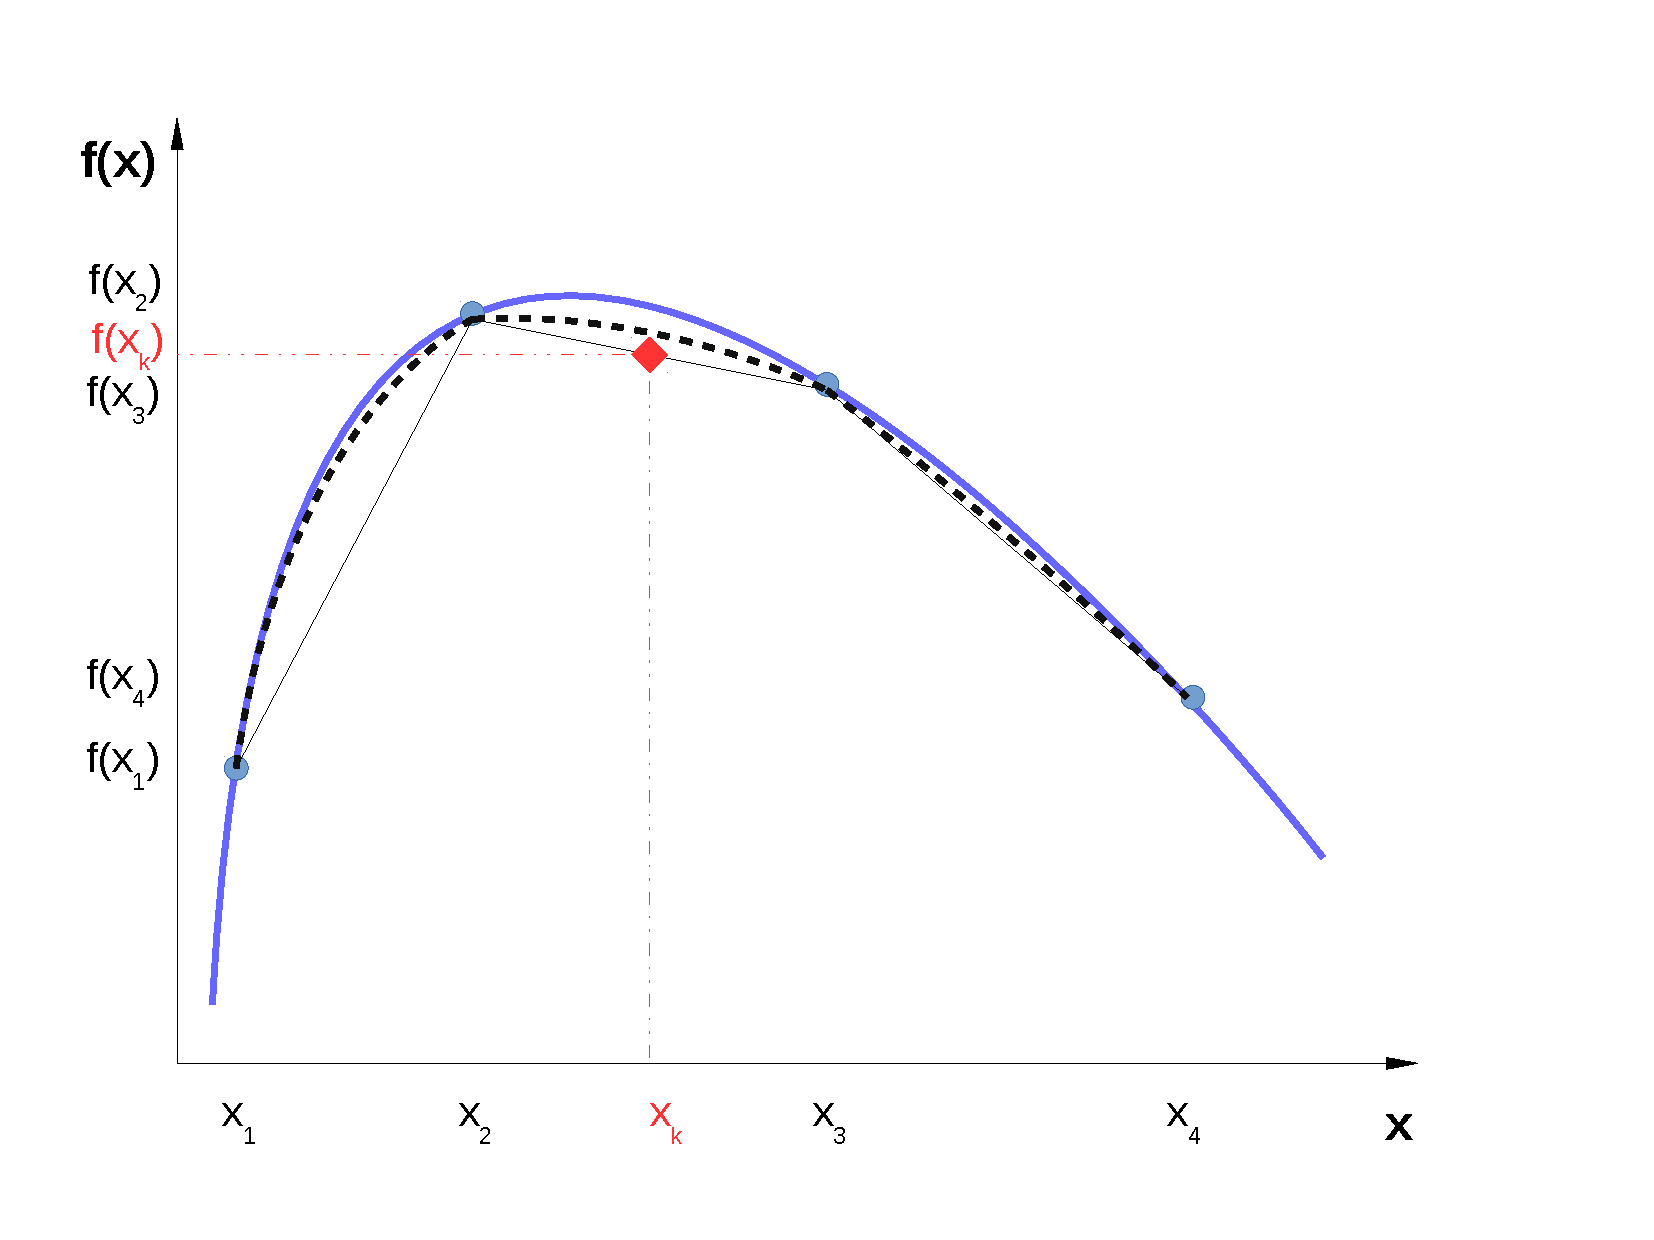
\includegraphics[width=\columnwidth,clip]{./../Pics/Interpolation}
           \caption{Smooth function $f(x)$ (solid blue line) may be more accurately interpolated by a high-order polynomial (black dotted line) than by a low-order polynomial (solid black line).} 
        \end{center}
      \end{figure}

   % Example
   \begin{MyExample}{\begin{center}{\bf Example}\end{center}}
      \begin{example}
         Given a table of values for $f(x)=\tan{x}$ for a few values of $x$,
            \begin{center}
               \begin{tabular}{c | c c c c}
                   $x$        & 1.00   & 1.10   & 1.20   & 1.30   \\
                   \hline
                   $\tan{x}$  & 1.5574 & 1.9648 & 2.5722 & 3.6021 \\
               \end{tabular}
            \end{center}
            Estimate $\tan{(1.15)}$ and $\tan{(1.23)}$.
     \end{example}

% SOLUTION
       \noindent{\bf Solution:} For $\left(x_{a}=1.10\right) < \left(x_{k}=1.15\right) < \left(x_{b}=1.20\right)$,
               \begin{eqnarray}
                  f\left(x_{k}\right) &=& \frc{f\left(x_{a}\right)\left(x_{b}-x_{k}\right) + f\left(x_{b}\right)\left(x_{k}-x_{a}\right)}{x_{b}-x_{a}} \nonumber \\
                                     &=& \frc{1.9648\times(1.20-1.15) + 2.5722\times(1.15-1.10)}{1.20-1.10} = 2.2685 \nonumber
               \end{eqnarray}

For  $\left(x_{a}=1.20\right) < \left(x_{k}=1.23\right) < \left(x_{b}=1.30\right)$,
               \begin{eqnarray}
                  f\left(x_{k}\right) &=& \frc{f\left(x_{a}\right)\left(x_{b}-x_{k}\right) + f\left(x_{b}\right)\left(x_{k}-x_{a}\right)}{x_{b}-x_{a}} \nonumber \\
                                     &=& \frc{2.5722\times(1.30-1.23) + 3.6021\times(1.23-1.20)}{1.30-1.20} = 2.8812 \nonumber
               \end{eqnarray}
   \end{MyExample}

   % Example
   \begin{MyExample}{\begin{center}{\bf Example}\end{center}}
      \begin{example}
         Calculate specific volume $\left(v, \text{in m}^{3}\text{.kg}^{-1}\right)$, internal energy $\left(u, \text{in kJ.kg}^{-1}\right)$ and entropy $\left(s, \text{in kJ.(kg.K)}^{-1}\right)$ of saturated water vapour at 133.45$^{\circ}$C.
     \end{example}

% SOLUTION
       \noindent{\bf Solution:} From Appendix~\ref{Appendix:Saturated_SH_Tables} (Table A-2), for $T_{a}(=130.0) < T_{k} (= 133.45) < T_{b} (=140.0)^{\circ}C$, thus:
               \begin{eqnarray}
                  v\left(T_{k}\right) &=& \frc{v\left(T_{a}\right)\left(T_{b}-T_{k}\right) + v\left(T_{b}\right)\left(T_{k}-T_{a}\right)}{T_{b}-T_{a}} \nonumber \\
                                     &=& \frc{0.6685\times(140.0-133.45) + 0.5089\times(133.45-130.0)}{140.0-130.0} = 0.6134 \text{ m}^{3}\text{.kg}^{-1}\nonumber \\
                                     && \nonumber \\
                  u\left(T_{k}\right) &=& \frc{u\left(T_{a}\right)\left(T_{b}-T_{k}\right) + u\left(T_{b}\right)\left(T_{k}-T_{a}\right)}{T_{b}-T_{a}} \nonumber \\
                                     &=& \frc{2539.9\times(140.0-133.45) + 2550.0\times(133.45-130.0)}{140.0-130.0} = 2543.39 \text{ kJ.kg}^{-1}\nonumber \\
                                     && \nonumber \\
                  s\left(T_{k}\right) &=& \frc{s\left(T_{a}\right)\left(T_{b}-T_{k}\right) + s\left(T_{b}\right)\left(T_{k}-T_{a}\right)}{T_{b}-T_{a}} \nonumber \\
                                     &=& \frc{7.0269\times(140.0-133.45) + 6.9299\times(133.45-130.0)}{140.0-130.0} = 6.9934 \text{ kJ.}\left(\text{kg.K}\right)^{-1}\nonumber 
               \end{eqnarray}
   \end{MyExample}


%%%
%%% SECTION
%%%
\section{Root-Finder Methods}\label{Section:RootFinderMethods}\index{Root-Finder Methods}

%%% SUBSECTION
\subsection{Motivation}
Given a smooth, {\it continuous} and {\it fully differentiable} function 
  \begin{displaymath}
     y = f(x) \hspace{3cm} \text{ with } x\in\mathbb{R}.
  \end{displaymath}
We aim to find the root $x=\psi$ of the function 
  \begin{displaymath}
     f(x) = 0.
  \end{displaymath}
The first step is to estimate $x_{0}$ that results in $f\left(x_{0}\right)\neq 0$ and may lead to a new estimate $x_{1}$. The procedure is repeated until $f\left(x_{n}\right)\rightarrow 0$ (\ie $x_{n}\approx\psi$), where $n$ is the number of repetitions (or {\it iterations}). There are several methods designed to solve non-linear equations, i.e., find the rrot of the function, here we will focus on the most popular {\it Newton-Raphson} method that combines simplicity and power.


%%% SUBSECTION
\subsection{Newton-Raphson Iterative Method}\label{Section:RootFinderMethods:NewtonRaphson}\index{Root-Finder Methods!Newton-Raphson method}
Let's assume that $x_{0}$ is a good estimate of the root$\psi$ and $\psi = x_{0} + h$. Since the root of the function $f(x)$ is $\psi$ and $h = \psi 0 x_{0}$, $h$ represents the distance between the initial estimate (or guess) and the root. Assuming $h$ is very (or {\it infinitesimal}) small, we can linearly approximate the function,
   \begin{displaymath}
        f\left(\psi\right) = 0 = f\left(x_{0}+h\right) \approx f\left(x_{0}\right) + h f'\left(x_{0}\right).
   \end{displaymath}
Therefore, except if $f'\left(x_{0}\right)$ is close to $0$, 
   \begin{displaymath}
        h \approx -\frc{f\left(x_{0}\right)}{f'\left(x_{0}\right)} \hspace{.3cm} \Longrightarrow \hspace{.3cm} \psi = x_{0} + h \approx x_{0} -\frc{f\left(x_{0}\right)}{f'\left(x_{0}\right)}.
   \end{displaymath}
%%% Figure
     \begin{figure}[h]\label{Appendix:Fig:NewtonRaphson}%
        \begin{center}
         \vbox{
           \hbox{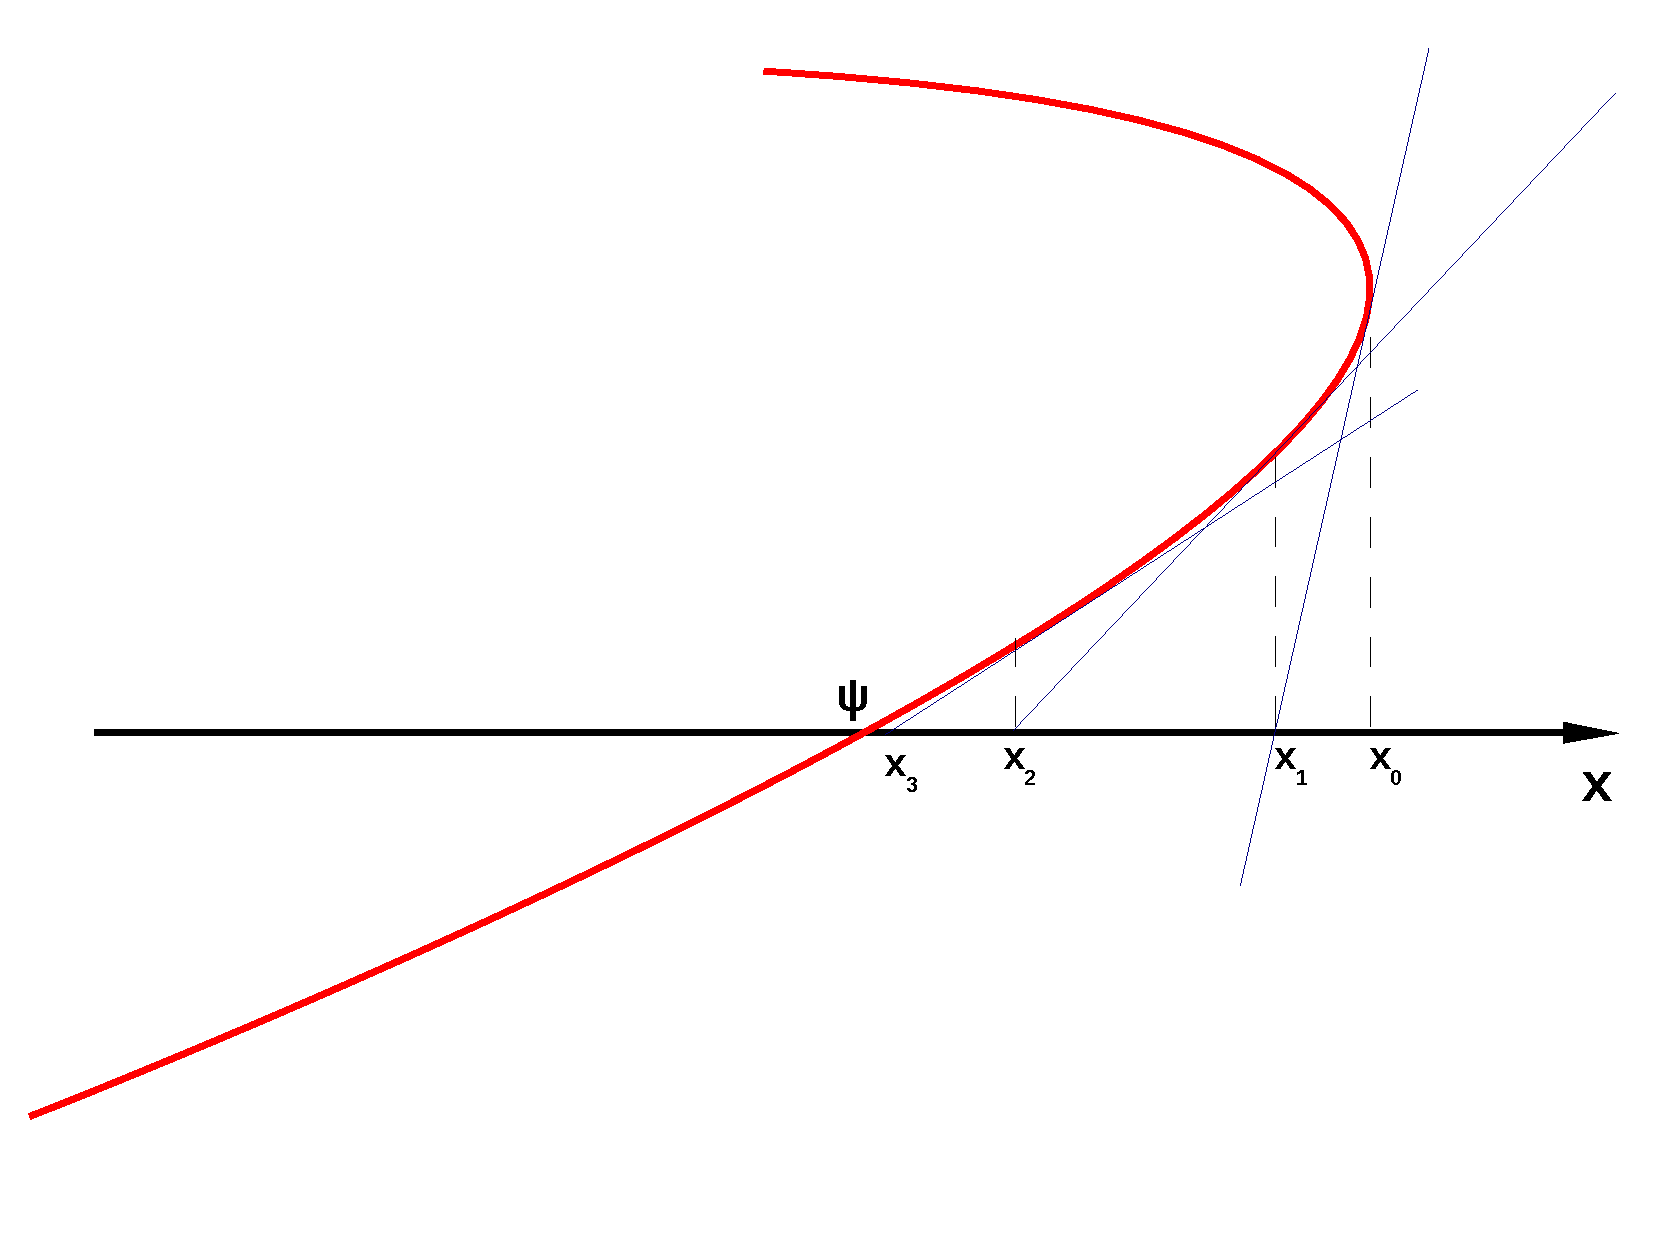
\includegraphics[width=\columnwidth,height=10cm]{./../Pics/NewtonRaphson2}}
           \hbox{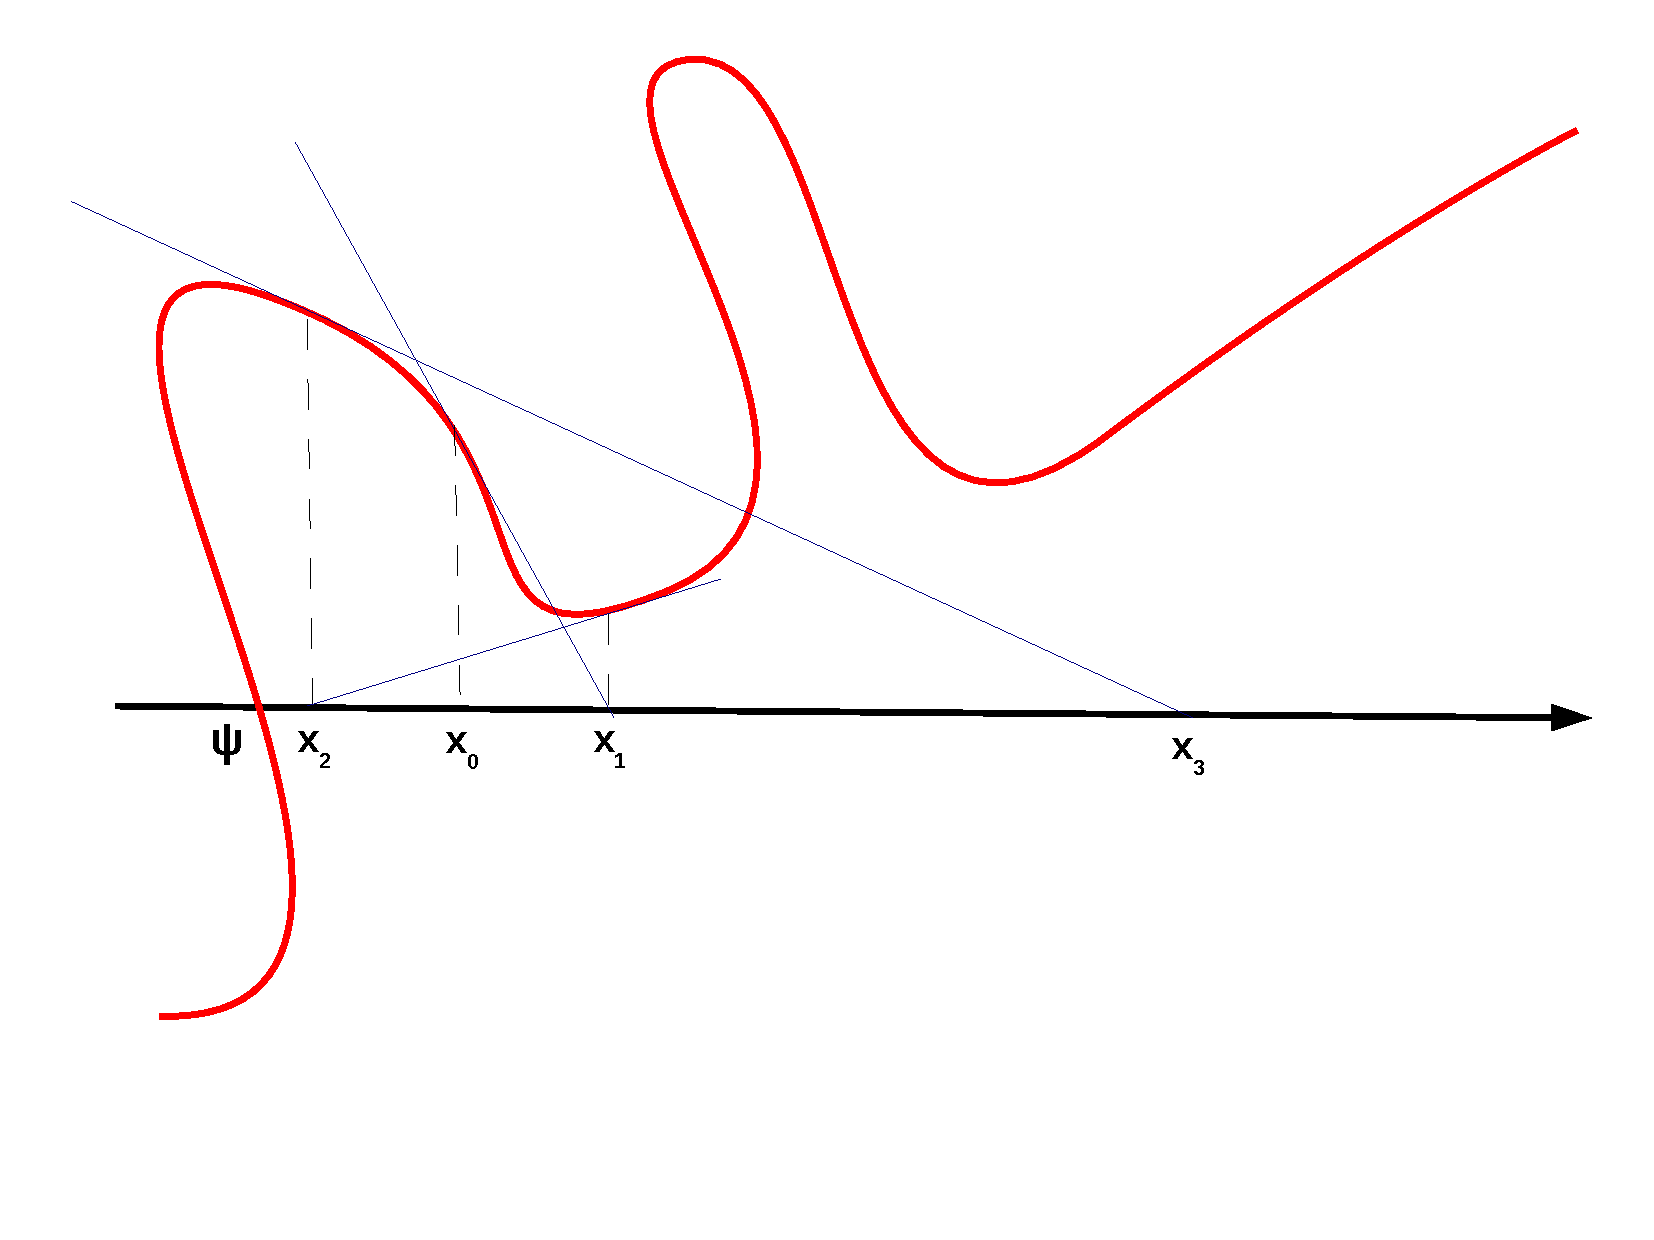
\includegraphics[width=\columnwidth,height=10cm]{./../Pics/NewtonRaphson3}}}
           \vspace{-1cm}
           \caption{Graphic representation of the Newton-Raphson iterative method: (top) solution of the smooth and continuous function $f(x)$ (solid red line) is approximated from the initial estimate $x_{0}$ to the final solution $x=\psi$; (bottom) initial estimate $x_{0}$ is far away from the root $\psi$ and the solution may diverge. Blue solid lines are tangent of the function at $x_{i}$.} 
        \end{center}
      \end{figure}
%
This expression represents an improvement of the original estimate, i.e.,  
   \begin{displaymath}
        x_{1} = x_{0} -\frc{f\left(x_{0}\right)}{f'\left(x_{0}\right)}.
   \end{displaymath}
The next estimate, $x_{2}$, is obtained from $x_{1}$, 
   \begin{displaymath}
        x_{2} = x_{1} -\frc{f\left(x_{1}\right)}{f'\left(x_{1}\right)}.
   \end{displaymath}

   \begin{shaded}
      We can generalise this expression for the $n-${\it th iteration},
         \begin{equation}
            x_{n+1} = x_{n} -\frc{f\left(x_{n}\right)}{f'\left(x_{n}\right)}.\label{NewtonRaphson:Eqn1}
         \end{equation}
   \end{shaded}

Figure~\ref{Appendix:Fig:NewtonRaphson}(a) shows a geometrical representation of the Newton-Raphson iterative method, where $m=f(x)$ is the tangent (blue) line at the coordinate pair $\left[x_{0},f\left(x_{0}\right)\right]$,
   \begin{displaymath}
     m = f\left(x_{0}\right) + \left(x-x_{0}\right)f'\left(x_{0}\right).
   \end{displaymath}
Let $x_{1}$ be the {\it x-intercept} of the tangent line, therefore
   \begin{displaymath}
     x_{1} = x_{0} - \frc{f\left(x_{0}\right)}{f'\left(x_{0}\right)}
   \end{displaymath}
The tangent line is a geometrical representation of the Newton-Raphson iterative method, Eqn.~\ref{NewtonRaphson:Eqn1}, as the estimates gradually tend to the root $\psi$ of the function. As it can be seen in the Fig.~\ref{Appendix:Fig:NewtonRaphson}(b), if the initial estimate $x_{0}$ is not close enough of the root $\psi$, the solution may not {\it converge}. In fact, the Newton-Raphson iterative method works most of the time if the initial estimate is {\it good enough}.

 From the {\it mean value theorem} (Theorem~\ref{Appendix:MeanValueTheorem}), let the function $f(x)$ be such that, 
   \begin{enumerate}[(a)]
      \item it is continuously differentiable in some open interval containing the solution $x=\psi$;
      \item $\left|f'(\psi)\right| < 1$.
   \end{enumerate}
Then there is a number $\epsilon > 0$ such that the iteration $x_{k+1}=f\left(x_{k}\right)$ {\it converges} whenever $x_{0}$ is chosen in $\left|x_{0}-\psi\right|\leq\epsilon$.

For bounded $x\in\mathbb{R}$ (\ie contained in the interval $a\leq x \leq b$), if $f''(x)$ exists and is continuous on $[a,b]$ and $\psi$ is a root of $f(x)$, that is, $f(\psi)=0$ and $f'(\psi)\neq0$. Thus for a function $g(x)$
    \begin{displaymath}
        g(x) = x - \frc{f(x)}{f'(x)}
    \end{displaymath}
with
    \begin{displaymath}
        g'(x) = 1 - \frc{[f'(x)]^{2} - f(x)f''(x)}{[f'(x)]^{2}} = \frc{f(x)f''(x)}{[f'(x)]^{2}},
    \end{displaymath}
and
    \begin{displaymath}
        g'(\psi) = \frc{f(\psi)f''(\psi)}{[f'(\psi)]^{2}}=0, \text{ since } f(\psi) = 0 \text{ and } f'(\psi) \neq 0
    \end{displaymath}
As $g'(x)$ is continuous, this means that there is a small neighbourhood around the root $x=\psi$ such that for all points $x$ in that neighbourhood, $\left|g'(x)\right|<1$.  Therefore, if $g(x)$ is chosen as above and the initial estimate $x_{0}$ is chosen {\it sufficiently close to the root} $x=\psi$, then the Newton-Raphson method is {\it guaranteed to converge}. 

Algorithm~\ref{Algorithm:NewtonRaphson} highlights the steps towards find the root of a function $f(x)$.

\begin{algorithm}[h]%\scriptsize
   \SetKwData{Left}{left}\SetKwData{This}{this}\SetKwData{Up}{up}
   \SetKwFunction{Union}{Union}\SetKwFunction{FindCompress}{FindCompress}
   \SetKwInOut{Input}{Input}\SetKwInOut{Output}{Output}\SetKwInOut{Calculate}{Calculate}\SetKwInOut{Set}{Set}\SetKwInOut{Adjust}{Adjust}\SetKwInOut{Assumption}{Assumption}

      \Input{Given the function $f(x)$, the initial estimate $x_{0}$, the error tolerance $\epsilon$ and the maximum number of iterations $N$:}
      \Output{An approximation to the root $x=\psi$}

      \Assumption{$x=\psi$ is a root of $f(x)$}

      \For{$k \leftarrow 0$ \KwTo $N$}{
             \Calculate{ $f\left(x_{k}\right)$ and $f'\left(x_{k}\right)$ }

             \Calculate{ $x_{k+1} = x_{k} - \frc{f\left(x_{k}\right)}{f'\left(x_{k}\right)}$ }

             \eIf{ $k == N$}{
                             {\it Calculation has \underline{not converged}. Modify the initial estimate $x_{0}$.} 
                   }{
                     \If{ $\left|f\left(x_{k}\right)\right| \leq \epsilon$ {\bf or} $\frc{\left|x_{k+1}-x_{k}\right|}{\left|x_{k}\right|} \leq \epsilon$ }{
                          {\it Stopping criteria} achieved. The root of function $f(x)$ is $\psi = x_{k+1}$
                          } }
          }
 \caption{Newton-Raphson method algorithm.}\label{Algorithm:NewtonRaphson}
\end{algorithm}

%%% SUBSECTION
\subsection{Secant Iterative Method}\label{Section:RootFinderMethods:Secant}\index{Root-Finder Methods!Secant method}
The Secant method is essentially the same as Newton-Raphson, however the derivative $f'(x)$ is approximated by a finite difference based on the current and the previous estimate for the root,
   \begin{displaymath}
       f'\left(x_{n}\right) \approx \frc{f\left(x_{n}\right) - f\left(x_{n-1}\right)}{x_{n}-x_{n-1}}
   \end{displaymath}

   \begin{shaded}
      Replacing the derivative in Eqn.~\ref{NewtonRaphson:Eqn1} for the $(n+1)^{\text{th}}$-{\it iteration},
         \begin{equation}
            x_{n+1} = x_{n} - \frc{ x_{n} - x_{n-1} }{f\left(x_{n}\right) - f\left(x_{n-1}\right)} f\left(x_{n}\right).\label{Secant:Eqn1}
         \end{equation}
   \end{shaded}
The main problem of the Secant iterative method is that it requires two initial estimates $x_{1}$ and $x_{0}$ for the calculations. These estimates must bound the solution, \ie, $x_{0} \leq \psi \leq x_{1}$. Algorithm~\ref{Algorithm:Secant} shows the steps for its implementation.


\begin{algorithm}[h]%\scriptsize
   \SetKwData{Left}{left}\SetKwData{This}{this}\SetKwData{Up}{up}
   \SetKwFunction{Union}{Union}\SetKwFunction{FindCompress}{FindCompress}
   \SetKwInOut{Input}{Input}\SetKwInOut{Output}{Output}\SetKwInOut{Calculate}{Calculate}\SetKwInOut{Set}{Set}\SetKwInOut{Adjust}{Adjust}\SetKwInOut{Assumption}{Assumption}

      \Input{Given the function $f(x)$, the initial estimates $x_{0}$ and $x_{1}$, the error tolerance $\epsilon$ and the maximum number of iterations $N$:}
      \Output{An approximation to the root $x=\psi$}

      \Assumption{$x=\psi$ is a root of $f(x)$}

      \For{$k \leftarrow 1$ \KwTo $N$}{
             \Calculate{ $f\left(x_{k}\right)$ and $f\left(x_{k-1}\right)$ }

             \Calculate{ $x_{k+1} = x_{k} - \frc{f\left(x_{k}\right)\left(x_{k}-x_{k-1}\right)}{f\left(x_{k}\right) - f\left(x_{k-1}\right)}$ }

             \eIf{ $k == N$}{
                             {\it Calculation has \underline{not converged}. Modify the initial estimate $x_{0}$.} 
                   }{
                     \If{ $\left|f\left(x_{k}\right)\right| \leq \epsilon$ {\bf or} $\frc{\left|x_{k+1}-x_{k}\right|}{\left|x_{k}\right|} \leq \epsilon$ }{
                          {\it Stopping criteria} achieved. The root of function $f(x)$ is $\psi = x_{k+1}$
                          } }
          }
 \caption{Secant method algorithm.}\label{Algorithm:Secant}
\end{algorithm}

   % Example
   \begin{MyExample}{\begin{center}{\bf Example}\end{center}}
     \begin{example}\label{Section:RootFinderMethods:Example:Roots:Secant} 
        Calculate the root of the function $f(x) = x^{2}-2$ using the Secant iterative method with initial estimates of $x_{0}=1.5$ and $x_{1}=1.0$. The error tolerance is $\epsilon=10^{-5}$.
     \end{example}

% SOLUTION
       \noindent{\bf Solution:} The Secant method is expressed through Eqn.~\ref{Secant:Eqn1} for the $(k+1)^{\text{th}}$-iteration,
          \begin{displaymath}
            x_{k+1} = x_{k} - \frc{ x_{k} - x_{k-1} }{f\left(x_{k}\right) - f\left(x_{k-1}\right)} f\left(x_{k}\right).
         \end{displaymath}
         \begin{list}{{\bf Iteration \arabic{mcounter}} (k=\arabic{mcounter}):~}{\usecounter{mcounter}}
            \item Calculating $x_{2}$ from $x_{0}$ and $x_{1}$:
                  \begin{eqnarray}
                      x_{2} &=& x_{1} - \frc{ x_{1} - x_{0} }{f\left(x_{1}\right) - f\left(x_{0}\right)} f\left(x_{1}\right) \nonumber \\
                           &=& 1 - \frc{1 - 1.5}{-1-0.25}  (-1) = 1.4 \nonumber 
                  \end{eqnarray}
                  Stoppage criteria:
                    \begin{enumerate}[(a)]
                         \item $\left|f\left(x_{2}\right)\right| = 0.04 \leq \epsilon \hspace{2cm} \Longrightarrow$ \underline{False}
                         \item $\frc{\left|x_{2}-x_{1}\right|}{\left|x_{1}\right|} = 0.0667 \leq \epsilon \hspace{1.4cm} \Longrightarrow$ \underline{False}
                    \end{enumerate}
            \item Calculating $x_{3}$ from $x_{1}$ and $x_{2}$:
                  \begin{eqnarray}
                      x_{3} &=& x_{2} - \frc{ x_{2} - x_{1} }{f\left(x_{2}\right) - f\left(x_{1}\right)} f\left(x_{2}\right) \nonumber \\
                           &=& 1.4 - \frc{1.4 - 1.0}{-0.04-(-1)}  (-0.04) = 1.4167\nonumber
                  \end{eqnarray}
                  Stoppage criteria:
                    \begin{enumerate}[(a)]
                         \item $\left|f\left(x_{3}\right)\right| = 0.0070 \leq \epsilon \hspace{2cm} \Longrightarrow$ \underline{False}
                         \item $\frc{\left|x_{3}-x_{2}\right|}{\left|x_{2}\right|} = 0.0193 \leq \epsilon \hspace{1.65cm} \Longrightarrow$ \underline{False}
                    \end{enumerate}
            \item Calculating $x_{4}$ from $x_{2}$ and $x_{3}$:
                  \begin{eqnarray}
                      x_{4} &=& x_{3} - \frc{ x_{3} - x_{2} }{f\left(x_{3}\right) - f\left(x_{2}\right)} f\left(x_{3}\right) \nonumber \\
                           &=& 1.4167 - \frc{1.4167 - 1.4}{0.0070-(-0.04)}  (0.0070) = 1.4142\nonumber
                  \end{eqnarray}
                  Stoppage criteria:
                    \begin{enumerate}[(a)]
                         \item $\left|f\left(x_{4}\right)\right| = 3.84\times 10^{-5} \leq \epsilon \hspace{2cm} \Longrightarrow$ \underline{False}
                         \item $\frc{\left|x_{4}-x_{3}\right|}{\left|x_{3}\right|} = 1.76\times 10^{-3} \leq \epsilon \hspace{1.65cm} \Longrightarrow$ \underline{False}
                    \end{enumerate}
            \item Calculating $x_{5}$ from $x_{3}$ and $x_{4}$:
                  \begin{eqnarray}
                      x_{5} &=& x_{4} - \frc{ x_{4} - x_{3} }{f\left(x_{4}\right) - f\left(x_{3}\right)} f\left(x_{4}\right) \nonumber \\
                           &=& 1.4142 - \frc{1.4142 - 1.4167}{-3.84\times 10^{-5}-(0.0070)}  (-3.84\times 10^{-5}) = 1.4142\nonumber
                  \end{eqnarray}
                  Stoppage criteria:
                    \begin{enumerate}[(a)]
                         \item $\left|f\left(x_{5}\right)\right| = 3.84\times 10^{-5} \leq \epsilon \hspace{2cm} \Longrightarrow$ \underline{False}
                         \item $\frc{\left|x_{5}-x_{4}\right|}{\left|x_{4}\right|} = 0.0 \leq \epsilon \hspace{3cm} \Longrightarrow$ \red{\underline{True}}
                    \end{enumerate}
         \end{list}
         Thus, \underline{4 iterations} were necessary to calculate the root of the function $f(x)=x^{2}-2$. The root of the function is \underline{$x=\psi=1.4142$}.
   \end{MyExample}
         

   % Example
   \begin{MyExample}{\begin{center}{\bf Example}\end{center}}
     \begin{example}\label{Section:RootFinderMethods:Example:Roots:NewtonRaphson} 
         Calculate the root of the same function of the previous example using the Newton-Raphson method.
     \end{example}

% SOLUTION
       \noindent{\bf Solution:} Now that we know the solution of the function, let's take the initial estimate as $x_{1}=1.5$. Newton-Raphson method is expressed through Eqn.~\ref{NewtonRaphson:Eqn1} for the $(k+1)^{\text{th}}$-iteration,
          \begin{displaymath}
            x_{k+1} = x_{k} - \frc{f\left(x_{k}\right)}{f'\left(x_{k}\right)}, \text{ where } f'\left(x_{k}\right) = 2x_{k}.
         \end{displaymath}
         \begin{list}{{\bf Iteration \arabic{qcounter}} (k=\arabic{qcounter}):~}{\usecounter{qcounter}}
            \item Calculating $x_{2}$ from $x_{1}$:
                  \begin{eqnarray}
                      x_{2} &=& x_{1} - \frc{f\left(x_{1}\right)}{f'\left(x_{1}\right)} = x_{1} - \frc{ x_{1}^{2}-2 }{ 2x_{1}}   \nonumber \\
                           &=& 1.5 - \frc{0.25}{3} = 1.4167\nonumber
                  \end{eqnarray}
                  Stoppage criteria:
                    \begin{enumerate}[(a)]
                         \item $\left|f\left(x_{2}\right)\right| = 0.0070 \leq \epsilon \hspace{2cm} \Longrightarrow$ \underline{False}
                         \item $\frc{\left|x_{2}-x_{1}\right|}{\left|x_{1}\right|} = 0.0555 \leq \epsilon \hspace{1.4cm} \Longrightarrow$ \underline{False}
                    \end{enumerate}
            \item Calculating $x_{3}$ from $x_{2}$:
                  \begin{eqnarray}
                      x_{3} &=& x_{2} - \frc{f\left(x_{2}\right)}{f'\left(x_{2}\right)} = x_{2} - \frc{ x_{2}^{2}-2 }{ 2x_{2}}  \nonumber \\
                           &=& 1.4167 - \frc{0.0070}{2.8334} = 1.4142\nonumber
                  \end{eqnarray}
                  Stoppage criteria:
                    \begin{enumerate}[(a)]
                         \item $\left|f\left(x_{3}\right)\right| = 3.84\times 10^{-5} \leq \epsilon \hspace{2cm} \Longrightarrow$ \underline{False}
                         \item $\frc{\left|x_{3}-x_{2}\right|}{\left|x_{2}\right|} = 1.77\times 10^{-3} \leq \epsilon \hspace{1.65cm} \Longrightarrow$ \underline{False}
                    \end{enumerate}
            \item Calculating $x_{4}$ from $x_{3}$:
                  \begin{eqnarray}
                      x_{4} &=& x_{3} - \frc{f\left(x_{3}\right)}{f'\left(x_{3}\right)} = x_{3} - \frc{ x_{3}^{2}-2 }{ 2x_{3}} \nonumber \\
                           &=& 1.4142 - \frc{-3.84\times 10^{-5}}{2.8284} = 1.4142\nonumber
                  \end{eqnarray}
                  Stoppage criteria:
                    \begin{enumerate}[(a)]
                         \item $\left|f\left(x_{4}\right)\right| = 3.84\times 10^{-5} \leq \epsilon \hspace{2cm} \Longrightarrow$ \underline{False}
                         \item $\frc{\left|x_{4}-x_{3}\right|}{\left|x_{3}\right|} = 0 \leq \epsilon \hspace{3.3cm} \Longrightarrow$ \red{\underline{True}}
                    \end{enumerate}
         \end{list}
         Thus, we need \underline{3 iterations} to calculate the root, \underline{$x=\psi=1.4142$}, of the function. Now try to use $x_{1}=1.0$ as a first estimate and check how many iterations will be necessary to convergence.

    You may have noticed that the function $f(x)=x^{2}-2$ has two real roots, $\sqrt{2}$ and $-\sqrt{2}$, and in the examples we only obtained the positive root. In order to find the negative root, we need to use initial estimates close enough to the solution, \eg $x_{0}=-1.5$·
   \end{MyExample}

         \setcounter{examplecounter}{0} 
       
\chapter{Table of Properties of Saturated and Superheated Fluids}\label{Appendix:Saturated_SH_Tables}

Extracted from~\cite{Moran_Book}.

  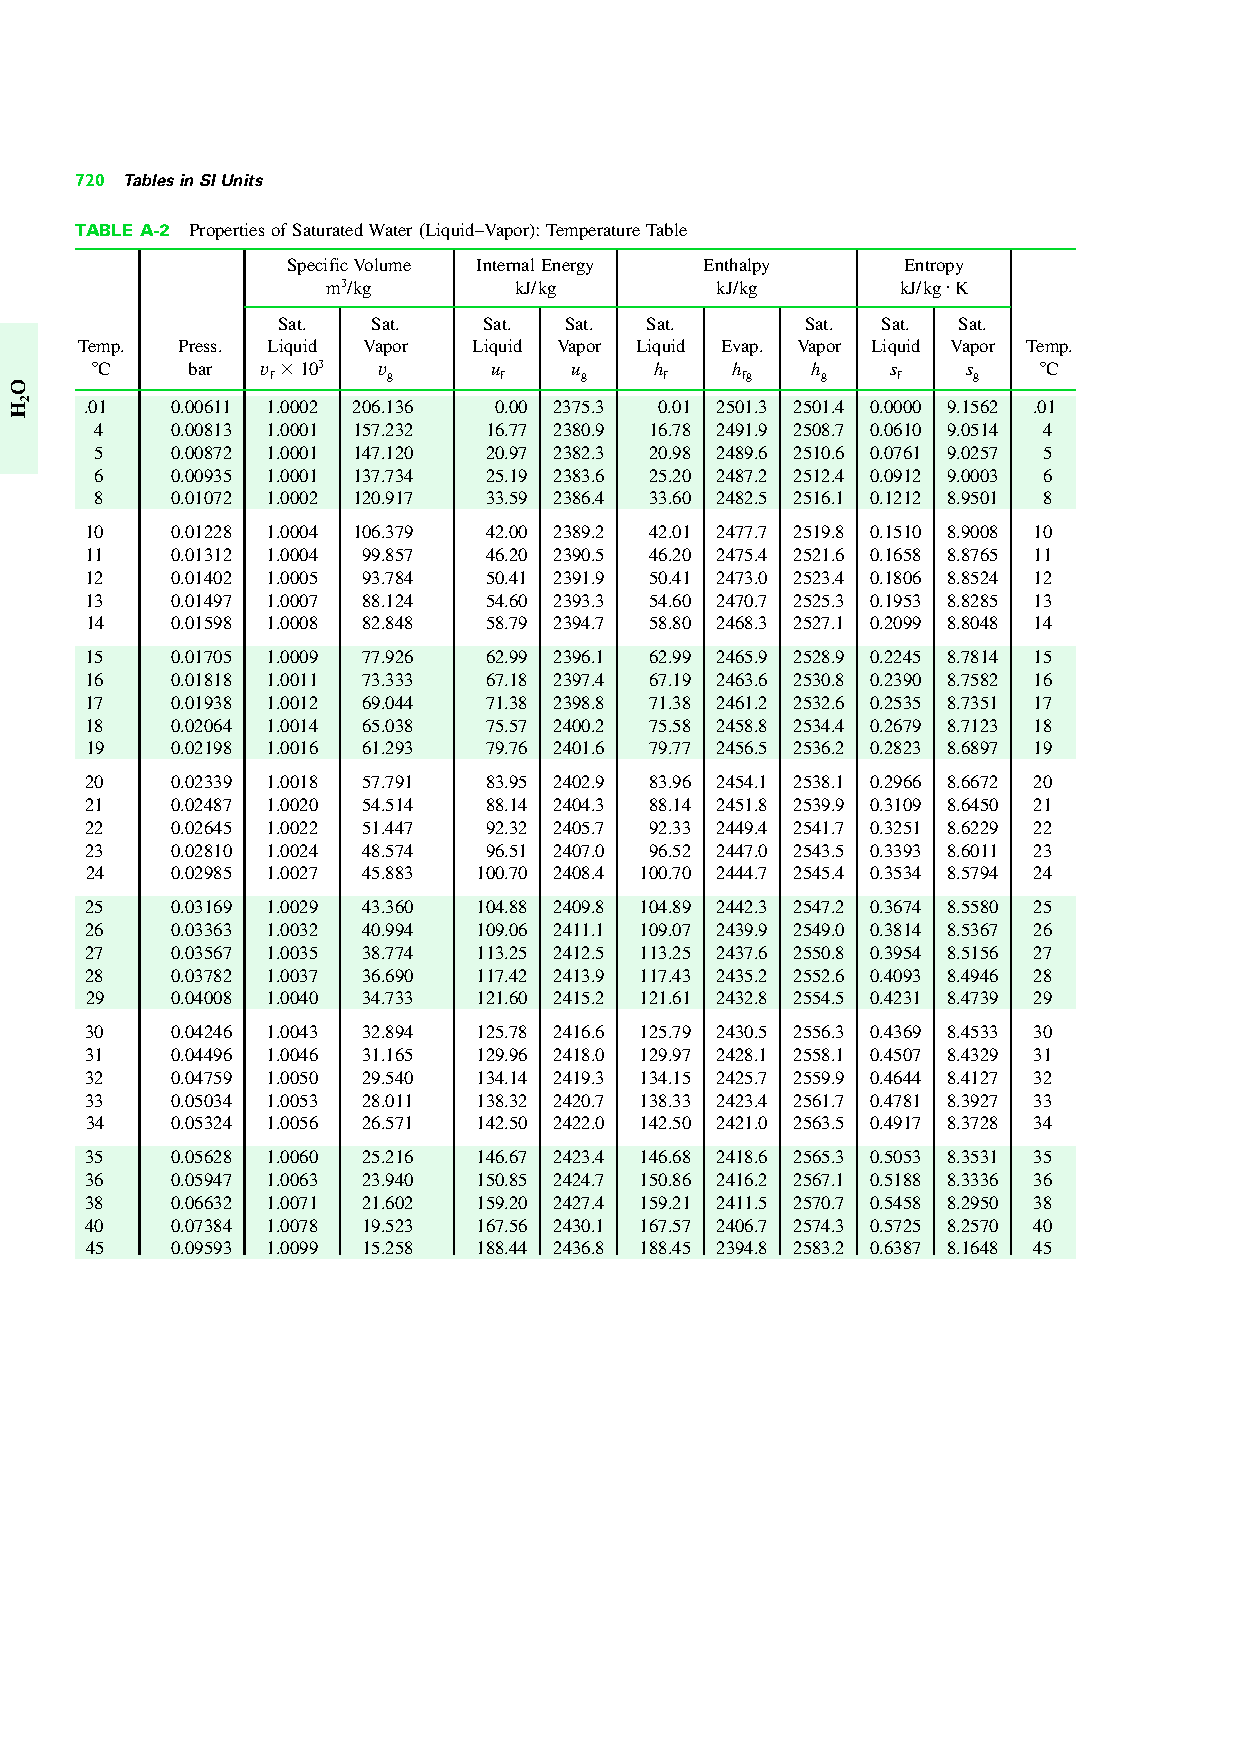
\includepdf[scale=1,pages=-,pagecommand={}, fitpaper]{./Pics/ChemEng_AllTables.pdf}

       %
\chapter{A Few Examples}

\section{Examples}

  \begin{list}{\bf Example \arabic{qcounter}:~}{\usecounter{qcounter}}
%
     %%% EXAMPLE 1:
     \item\label{example1} Using the cyclic rule (Appendix~\ref{Appendix_Calculus:Properties}) and the definitions,
    \begin{displaymath}
        \alpha = \frc{1}{V}\left(\frc{\partial V}{\partial T}\right)_{P} \hspace{1cm}\text{ and }\hspace{1cm} \beta = -\frc{1}{V}\left(\frc{\partial V}{\partial P}\right)_{T},
    \end{displaymath}
    \noindent show that 
    \begin{displaymath}
      \left(\frc{\partial P}{\partial T}\right)_{V} = \frc{\alpha}{\beta}.
    \end{displaymath}
%%
\medskip
     {\bf Solution:} From the cyclic rule,
       \begin{displaymath}
          \left(\frc{\partial P}{\partial T}\right)_{V}\left(\frc{\partial V}{\partial P}\right)_{T}\left(\frc{\partial T}{\partial V}\right)_{T} = -1.
       \end{displaymath}
     Thus,
       \begin{displaymath}
          \left(\frc{\partial P}{\partial T}\right)_{V} = \frc{-1}{\left(\frc{\partial V}{\partial P}\right)_{T}\left(\frc{\partial T}{\partial V}\right)_{T}} = \frc{-\left(\frc{\partial V}{\partial T}\right)_{P}}{\left(\frc{\partial V}{\partial P}\right)_{T}} = \frc{-V\alpha}{-V\beta} = \frc{\alpha}{\beta}
       \end{displaymath}
      
%
     %%% EXAMPLE 2:
     \item\label{example2} For a van der Waals gas, the pressure $P$ and the internal energy $U$ can be expressed as functions of the number of mols ($n$), total volume ($V$) and temperature ($T$),
       \begin{displaymath}
         P = \frc{n R T}{V-nb} - \frc{n^{2}a}{V^{2}} \hspace{1cm}\text{ and }\hspace{1cm} U = \frc{3}{2}n R T - \frc{n^{2}a}{V},
       \end{displaymath}
       respectively, where $a$ and $b$ are constants. Use these equations and the chain rule to derive an equation for $\left(\frc{\partial U}{\partial P}\right)_{n,T}$ in terms of $n$, $V$ and $T$.

%%
\medskip
{\bf Solution:}
   \begin{eqnarray}
      \Partial[U]{P}{n,T} &=& \Partial[U]{V}{n,T}\Partial[V]{P}{n,T} = \frc{\Partial[U]{V}{n,T}}{\Partial[P]{V}{n,T}} \nonumber \\
                          &=& \frc{\frc{n^{2}a}{V^{2}}}{\frc{2n^{2}a}{V^{3}}-\frc{n R T}{\left(V-nb\right)^{2}}} = \frc{n a}{\frc{2 n a}{V}-\frc{R T V^{2}}{\left(V-nb\right)^{2}}}\nonumber
   \end{eqnarray}
      
%
     %%% EXAMPLE 3:
     \item\label{example3} The heat capacity at constant volume is defined as $C_{v}\equiv \Partial[U]{T}{V}$. Show that
       \begin{displaymath}
          \Partial[U]{T}{P} = C_{v} + \alpha V\Partial[U]{V}{T},
       \end{displaymath}
       with $\alpha=\frc{1}{V}\Partial[V]{T}{P}$.

%
\medskip
       {\bf Solution:}
          \begin{displaymath}
            \Partial[U]{T}{P} = \Partial[U]{T}{V} + \Partial[U]{V}{T}\Partial[V]{T}{P},
          \end{displaymath}
          however $\Partial[U]{T}{V}=C_{v}$ and $\Partial[V]{T}{P}=V\alpha$. Thus,
          \begin{displaymath}
             \Partial[U]{T}{P} = C_{v} + \alpha V\Partial[U]{V}{T}.
          \end{displaymath}

%
     %%% EXAMPLE 4:
     \item\label{example4} h
%
\end{list}

\pagebreak

%%%
%%% SECTION
%%%
\section{Quiz}

  \begin{list}{\bf Question \arabic{qcounter}:~}{\usecounter{qcounter}}

%
     %%% QUESTION:
     \item\label{Q1} An experimentalist claims to have raised the temperature of a small amount of water to 150 C by transferring heat from a high temperature steam at 120 C. Is this a reasonable claim? Why? Assume no refrigerator/heat pump is used in the process. 
%

%\medskip
       {\bf Solution:} No. Heat cannot flow from a low temperature medium to a higher temperature medium.

%
     %%% QUESTION:
     \item\label{Q2} What is a thermal energy reservoir? Give examples.
%

%\medskip
       {\bf Solution:} A thermal energy reservoir is a body that can supply or absorb finite quantities of heat isothermally. Some examples are the oceans,lakes, and the atmosphere.
%
     %%% QUESTION:
     \item\label{Q3} Is it possible for a heat engine to operate without rejecting any waste heat to a low temperature reservoir? Explain.
%

%\medskip
       {\bf Solution:} No. Such an engine violates the Kelvin Planck statement of the second law of thermodynamics.

%
     %%% QUESTION:
     \item\label{Q4} What are the characteristics of all heat engines?
%

%\medskip
       {\bf Solution:} Heat engines are cyclic devices that receive heat from a source, convert some of it to work, and reject the rest to a sink.

%
     %%% QUESTION:
     \item\label{Q5} What is the Kelvin Planck expression of the second law of thermodynamics?
%

%\medskip
       {\bf Solution:} "No heat engine can exchange heat with a single reservoir and produce an equivalent amount of work" aka every pair of pants must have two legs
%
     %%% QUESTION:
     \item\label{Q6} Does a heat engine that has a thermal efficiency of 100 percent necessarily violate (a) the first law and (b) the second law of thermodynamics.
%

%\medskip
       {\bf Solution:} (a) No. (b) Yes. According the the second law of thermodynamics, no heat engine can have an efficiency of 100 percent.

%
     %%% QUESTION:
     \item\label{Q7} In the absence of any friction and other irreversibilities, an a heat engine have an efficiency of 100 percent? Explain
%

%\medskip
       {\bf Solution:} No. This violates the second law of thermodynamics.
%
     %%% QUESTION:
     \item\label{Q8} What is the difference between a refrigerator and a heat pump?
%

%\medskip
       {\bf Solution:}  The difference between the two is the purpose of each. The purpose of a refrigerator is to remove heat from a cold medium whereas the purpose of a heat engine is to supply heat to a warm medium.

%
     %%% QUESTION:
     \item\label{Q9} A heat pump is a device that absorbs energy from the cold outdoor air and transfers it to the warmer indoors. Is this a violation of the second law of thermodynamics? Explain.
%

%\medskip
       {\bf Solution:} No. Because the heat pump consumes work to accomplish this task
%
     %%% QUESTION:
     \item\label{Q10} Define the coefficient of performance of a refrigerator in words. Can is be greater than one? 
%

%\medskip
       {\bf Solution:} It represents the amount of heat removed from the refrigerated space for each unit of work supplied. It can be greater than 1

%
     %%% QUESTION:
     \item\label{Q11} A heat pump that is used to heat a house has a COP of 2.5. That is, the heat pump delivers 2.5 kWh of energy to the house for each 1 kWh of electricity it consumes. Does this violate the first law of thermodynamics?
%

%\medskip
       {\bf Solution:} No. The heat pump captures energy from a cold medium and carries it to a warm medium. It does not create it
%
     %%% QUESTION:
     \item\label{Q12} What is the Clausius expression of the second law of thermodynamics?
%

%\medskip
       {\bf Solution:} No device can transfer heat from a cold medium to a warm medium without requiring a heat or work input from the surroundings.

%
     %%% QUESTION:
     \item\label{Q13} Why are engineers interested in reversible processes even though they can never be achieved?
%

%\medskip
       {\bf Solution:} Because reversible processes can be approached in reality, and they form the limiting cases. Work producing devices that operate on reversible processes deliver the most work, and work consuming devices that operate on reversible processes consume the least amount of work.

%
     %%% QUESTION:
     \item\label{Q14} Why does a non-quasi equilibrium compression process require a larger work input than the corresponding quasi equilibrium one?
%

%\medskip
       {\bf Solution:}  When the compression process is non-quasi equilibrium, the molecules before the piston face cannot escape fast enough, forming a high pressure region in front of the piston. It takes more work to more the piston against this higher pressure region.
%
     %%% QUESTION:
     \item\label{Q15} Is a reversible expansion or compression process necessarily quasi equilibrium? Is a quasi equilibrium expansion or compression necessarily reversible?
%

%\medskip
       {\bf Solution:}  A reversible expansion or compression process cannot involve unrestained expansion or sudden compression, and thus it is quasi equilibirum. A quasi equilibirum expansion or compression process, on the other hand, may involve external irreversibilities (like heat transfer through a finite temperature difference) nad thus is not necessarily reversible.

%
     %%% QUESTION:
     \item\label{Q16} What are the four processes that make up the Carnot cycle?
%

%\medskip
       {\bf Solution:}  Isothermal expansion, reversible adiabatic expansion, isothermal compression, reversible adiabatic compression

%
     %%% QUESTION:
     \item\label{Q17} What are the two statements known as the Carnot principles? 
%

%\medskip
       {\bf Solution:} 1. Thermal efficiency of an irreversible heat engine is lower thant the efficiency of a reversible heat engine operating between the same two reservoirs; 2. The thermal efficiency of all the reversible heat engines operating between the same two reservoirs are equal

%
     %%% QUESTION:
     \item\label{Q18} Somebody claims to have developed a new reversible heat engine cycle that has a higher theoretical efficiency than the Carnot cycle operating between the same temperature limits. Is this a reasonable claim? 
%

%\medskip
       {\bf Solution:} No. The second Carnot principle states that no heat engine cycle can have a higher thermal efficiency than the Carnot cycle operating between the same temperature limits.

%
     %%% QUESTION:
     \item\label{Q19} Is it possible to develop (a) an actual and (b) a reversible heat engine cycle that is more efficient that a Carnot cycle operating between the same temperature limits? 
%

%\medskip
       {\bf Solution:} (a) No. (b) No. They would violate the Carnot Principles

%
     %%% QUESTION:
     \item\label{Q20} Somebody claims to have developed a new reversible heat engine that has the the same theoretical efficiency as the Carnot cycle operating between the same temperature limits? Is this a reasonable claim?
%

%\medskip
       {\bf Solution:} Yes. the second Carnot principle states that all reversible heat engine cycles operating between the same temperature limits have the same thermal efficiency.


%
     %%% QUESTION:
     \item\label{Q21} Consider two actual power plants operating with solar energy. Energy is supplied to one plant from a solar pond at 80 C and to the other from concentrating collectors that raise the water temperature to 600 C. Which of these power plants will have a higher efficiency?
%

%\medskip
       {\bf Solution:} The one that has a source temperature of 600 C. This is true because the higher the temperature at which heat is supplied to the working fluid of a heat engine, the higher the thermal efficiency.

%
     %%% QUESTION:
     \item\label{Q22} How can we increase COP of a Carnot refrigerator?
%

%\medskip
       {\bf Solution:} By increasing TL or decreasing TH

%
     %%% QUESTION:
     \item\label{Q23} What is the highest COP that a refrigerator operating between temperature levels TL and TH can have?
%

%\medskip
       {\bf Solution:} It is the COP that a Carnot refrigerator would have, COP=1/(TH/TL -1)

%
     %%% QUESTION:
     \item\label{Q24} In an effort the conserve energy in a heat engine cycle, somebody suggests incorporating a refrigerator that will absorb some of the waste energy QL and transfer it to the energy source of the heat engine. Is this a smart idea?
%

%\medskip
       {\bf Solution:} No. At best (when all is reversible), the increase in the work produced will be equal to the work consumed by the refrigerator. In reality, the work consumed by the refrigerator will always be greater than the additional work produced, resulting in a decrease in the thermal efficiency of the power plant.

%
     %%% QUESTION:
     \item\label{Q25} It is well established that the thermal efficiency of a heat engine increases as the temperature TL at which the heat is rejected from the heat engine decreases. In an effort to increase the efficiency of a power plant, somebody suggest refrigerating the cooling water before it enters the condenser, where heat rejection takes place. Would you be in favor of this idea? Why?
%

%\medskip
       {\bf Solution:} No. At best (when all is reversible), the increase in the work produced will be equal to the work consumed by the refrigerator. In reality, the work consumed by the refrigerator will always be greater than the additional work produced, resulting in a decrease in the thermal efficiency of the power plant.

%
     %%% QUESTION:
     \item\label{Q26} It is well known that the thermal efficiency of heat engines increases as the temperature of the energy source increases. In an attempt to improve the efficiency of a power plant, somebody suggest transferring heat from the available energy source to a higher temperature medium by a heat pump before energy is supplied to the power plant. What do you think of this suggestion?
%

%\medskip
       {\bf Solution:} Bad Idea. At best (all is reversible), the increase in the work produced will equal the work consumed by the heat pump. In reality, the work consumed by the heat pump will always be greater than the additional work produced, resulting in a decrease in the thermal efficiency of the power plant.

%
     %%% QUESTION:
     \item\label{Q27} Does the temperature in the Clausius inequality relation have to be absolute temperature? Why?
%

%\medskip
       {\bf Solution:} Yes. Because we used the relation (QH/TH=QL/TL) in the proof, which is the defining relation of absolute temperature.

%
     %%% QUESTION:
     \item\label{Q28} Does a cycle for which deltaQ>0 violate the Clausius inequality? 
%

%\medskip
       {\bf Solution:} No. The deltaQ represents the net heat transfer during a cycle, would could be positive

%
     %%% QUESTION:
     \item\label{Q29} Does the cyclic integral of heat have to be zero (i.e. does a system have to reject as much heat as it consumes to complete a cycle)? 
%

%\medskip
       {\bf Solution:} No. A system may reject more or less heat than it receives during a cycle. The steam in a steam power plant, for example, received more heat than it rejects in a cycle.

%
     %%% QUESTION:
     \item\label{Q30} Does the cyclic integral of work have to be zero (i.e. does a system have to produce as much work as it consumes to complete a cycle)? 
%

%\medskip
       {\bf Solution:} No. A system may produce more or less work than it receives during a cycle. A steam power plant for example, produces more work than it receives during a cycle, the difference being the the net work output.

%
     %%% QUESTION:
     \item\label{Q31} A system undergoes a process between two fixed states first in a reversible manner and then in an irreversible manner. For which case is the entropy change greater?
%

%\medskip
       {\bf Solution:} The entropy change will be the same for both cases since the entropy is a a property and it has a fixed value at a fixed state.

%
     %%% QUESTION:
     \item\label{Q32} Is the value of the integral, from 1 to 2, of deltaQ/T the same for all processes between states one and two?
%

%\medskip
       {\bf Solution:} No. In general, that integral will have a different value for different processes. However, it will have the same value for all reversible processes.

%
     %%% QUESTION:
     \item\label{Q33} Is the value of the integral, from 1 to 2, of deltaQ/T the same for all reversible processes between states one and two?
%

%\medskip
       {\bf Solution:} Yes

%
     %%% QUESTION:
     \item\label{Q34} To determine the entropy change for an irreversible process between states one and two, should the integral, from 1 to 2, of deltaQ/T be performed along the actual process path or an imaginary reversible path?
%

%\medskip
       {\bf Solution:} That integral would be performed along a reversible path to determine the entropy change

%
     %%% QUESTION:
     \item\label{Q35} Is an isothermal process necessarily internally reversible? Give an example.
%

%\medskip
       {\bf Solution:} No. An isothermal process and be irreversible. For example, a system that involves paddle wheel work while losing an equivalent amount of heat.

%
     %%% QUESTION:
     \item\label{Q36} How do the values of the integral, from 1 to 2, of deltaQ/T compare for a reversible and irreversible process between the same end states? 
%

%\medskip
       {\bf Solution:} The value of this integral is always larger for reversible processes

%
     %%% QUESTION:
     \item\label{Q37} A piston cylinder device contains helium gas. During a reversible, isothermal process, the entropy of the helium will increase ...
%

%\medskip
       {\bf Solution:} Sometimes

%
     %%% QUESTION:
     \item\label{Q38} A piston cylinder device contains nitrogen gas. During a reversible, adiabatic process, the entropy of the nitrogen will increase
%

%\medskip
       {\bf Solution:} Never

%
     %%% QUESTION:
     \item\label{Q39} A piston cylinder device contains superheated steam. During an actual, adiabatic process, the entropy of the steam will increase.
%

%\medskip
       {\bf Solution:} Always

%
     %%% QUESTION:
     \item\label{Q40} The entropy of steam will ... as it flows through an actual adiabatic turbine.
%

%\medskip
       {\bf Solution:} Increase

%
     %%% QUESTION:
     \item\label{Q41} The entropy of the working fluid of the ideal Carnot cycle ... during the isothermal heat addition process.
%

%\medskip
       {\bf Solution:} Increase

%
     %%% QUESTION:
     \item\label{Q42} The entropy of the working fluid of the ideal Carnot cycle ... during the isothermal heat rejection process
%

%\medskip
       {\bf Solution:} Decreases

%
     %%% QUESTION:
     \item\label{Q43} During a heat transfer process, the entropy of a system ... increases
%

%\medskip
       {\bf Solution:} Sometimes

%
     %%% QUESTION:
     \item\label{Q44} Is it possible for the entropy change of a closed system to be zero during an irreversible process?
%

%\medskip
       {\bf Solution:} Yes. This will happen when the system is losing heat, and the decrease in entropy as a result of this heat loss is equal in entropy as a result of irreversibilities.

%
     %%% QUESTION:
     \item\label{Q45} Is a process that is internally reversible and adiabatic necessarily isentropic? 
%

%\medskip
       {\bf Solution:} Yes, because an internally reversible, adiabatic process invovles no irreversibilities or heat transfer
%
     %%% QUESTION:
     \item\label{Q46} Consider two sold blocks, one hot and one cold, brought into contsant in an adiabatic container. After a while, thermal equilibrium is established in the container as a result of heat transfer. The first law requires that the amount of energy lost by the hot solid be equal to the amount of energy gained by the cold one. Does the second law require that the decrease in entropy of the hot solid be equal to the increase in entropy of the cold one?
%

%\medskip
       {\bf Solution:} No, because entropy is not a conserved property

%
     %%% QUESTION:
     \item\label{Q47} Can entropy of an ideal gas change during an isothermal process? 
%

%\medskip
       {\bf Solution:} The entorpy of a gas can change during an isothermal process since entropy of an ideal gas depends on the pressure as well as the temperature.

%
     %%% QUESTION:
     \item\label{Q48} An ideal gas undergoes a process between two specifes temperatures, first at constant pressure and then at constant volume. For which case will the ideal gas experience a larger entropy change? 
%

%\medskip
       {\bf Solution:} The entropy change relations of an ideal gas simplify to: 1. delta s=Cpln(T2/T1) for a constant pressure process 2. delta s=Cvln(T2/T1) for a constant volume process 3 noting that Cp>Cv. the entropy change will be larger for a constant pressure process

%
     %%% QUESTION:
     \item\label{Q49} Describe the ideal process for an (a) adiabatic turbine, (b) adiabatic compressor, and (c) adiabatic nozzle, and define the isentropic efficiency for each device.
%

%\medskip
       {\bf Solution:} The ideal process for all three devices is the reversible adiabatic (i.e. isentropic) process. The isentropic efficincies can be defined as: 1. eta(turbine, isentropic)= actual work output/isentropic work output 2. eta(compressor,isentopic)=isentropic work input/ actual work input 3. eta(nozzle,isentropic)=actual exit kinetic energy/ isentropic exit kinetic energy


%
     %%% QUESTION:
     \item\label{Q50} Is the isentropic process a suitable model for compressors that are cooled intentionally? 
%

%\medskip
       {\bf Solution:} No, because the isentropic process is not the model or ideal process for compressors that are cooled unintentionallly.

%
     %%% QUESTION:
     \item\label{Q51} On a T-s diagram, does the actual exit state (state 2) of an adiabatic turbine have to be on the right hand side of the isentropic exit state (state 2s)?
%

%\medskip
       {\bf Solution:} Yes. Because the entropy of the fluid must increase during an actual adiabatic process as a result of irreversibilities. Therefore, the actual exit state has to be on the right hand side of the isentropic exit state.

%
\end{list}

  \end{appendix}

\cleardoublepage

\pagebreak

\bibliographystyle{plainnat}
\bibliography{../refbib}
%\bibliographystyle{unsrt}

\cleardoublepage
\phantomsection
\renewcommand\leftmark{}
\renewcommand\rightmark{Index}
\addcontentsline{toc}{chapter}{Index}

\printindex


\end{document}
